% create and set switches
% needed for custom switches
\RequirePackage{etoolbox}

% ======================================================================
% Toggle Settings
% ======================================================================

% draftMode switch:
% show draft watermark, disabling overrides checkMode, debugMode, and
% showGlossaryDefinitionsMode (see below)
\newtoggle{draftMode}
\toggletrue{draftMode}

% checkMode switch:
% show all overfull/underfull boxes, show unknown hyphenations
\newtoggle{checkMode}
\toggletrue{checkMode}

% debugMode switch:
% show all boxes, glues, and kerning info
\newtoggle{debugMode}
\togglefalse{debugMode}

% showGlossaryDefinitionsMode switch:
% print definition of glossary entries in the text body
\newtoggle{showGlossaryDefinitionsMode}
\togglefalse{showGlossaryDefinitionsMode}

% flipBookMode switch:
% add flip book images in corners of page
\newtoggle{flipBookMode}
\togglefalse{flipBookMode}

% partialCompile switches:
% only compile a single chapter to save compilation time
\newtoggle{partialCompileMode}
\toggletrue{partialCompileMode}

% select chapters to compile for partialCompileMode = true
\includeonly{%
  %10introduction,
  20sparseGrids,
  %30BSplines,
  %40hierarchization,
  %50optimization,
  %60topoOpt,
  %70muscle,
  %80finance,
  %90conclusion,
  %a10proofs,
}

% ======================================================================
% Toggle Logic
% ======================================================================

% disable checkMode, showGlossaryDefinitionsMode, and debugMode
% if draftMode is disabled
\iftoggle{draftMode}{}{
  \togglefalse{checkMode}
  \togglefalse{debugMode}
  \togglefalse{showGlossaryDefinitionsMode}
}

% compile everything if partialCompileMode is disabled
\makeatletter
\iftoggle{partialCompileMode}{}{
  % disable the \includeonly mechanism
  \@partswfalse
}
\makeatother


% set main document class (KOMA-Script's scrbook)
\documentclass[
  % align equation numbers left to the equation
  leqno,
]{scrbook}

% include packages
% language-specific things (hyphenation, ...)
\usepackage[ngerman,american]{babel}

% biblatex package wants to have csquotes (otherwise: warning)
\usepackage{csquotes}

% lower-case page header
\usepackage[markcase=lower]{scrlayer-scrpage}

% dummy texts
\usepackage[math]{blindtext}

% basic AMS math commands
\usepackage{amsmath}

% micro-typographic adjustments
\usepackage[
  % don't deactivate extensions due to document class draft option
  final,
  % increase letter spacing in small-caps
  tracking=smallcaps,
  % smaller amount of letter spacing (default: 100)
  letterspace=50,
]{microtype}

% check mode
\iftoggle{checkmode}{
  % show non-whitelisted hyphenations
  \usepackage[mark]{lua-check-hyphen}
}{}

% debug mode
\iftoggle{debugmode}{
  % show boxes, glues, and kerning
  \usepackage{lua-visual-debug}
}{}

% Unicode umlauts
\usepackage[utf8]{luainputenc}

% use GoMono as typewriter font
\usepackage[scale=0.9]{GoMono}

% need T1 font encoding for Charter,
% otherwise there will be "undefined font shape" warnings
\usepackage[T1]{fontenc}

% use Bitstream Charter as main font
\usepackage[bitstream-charter]{mathdesign}

% graphics
\usepackage{graphicx}

% X column type for tables (filling rest of line)
\usepackage{tabularx}

% table of symbols and acronyms
\usepackage[
  % show glossary in table of contents
  toc,
  % don't group entries with same first letter
  nogroupskip,
  % don't append full stop to entries
  nopostdot,
  % don't append pages where the acronym is referenced
  nonumberlist,
]{glossaries}

% line spacing (one and a half lines)
\usepackage[onehalfspacing]{setspace}

% PDF links
\usepackage{hyperref}

% BibLaTeX
\usepackage{biblatex}

% named references
\usepackage{cleveref}


% set packages options
% ======================================================================
% Meta-Data
% ======================================================================

% meta-data variables
\newcommand*{\thetitle}{%
  B-Splines for Sparse Grids:\texorpdfstring{\\}{}
  Algorithms and Application to\texorpdfstring{\\}{}
  Higher-Dimensional Optimization%
}
\newcommand*{\theauthor}{Julian Valentin}
\newcommand*{\thebirthplace}{Stuttgart}
\newcommand*{\thedefensedate}{\todo{insert date of defense}}
\newcommand*{\thedate}{\todo{insert date}}
\newcommand*{\theyear}{2018}
\newcommand*{\theinstitute}{Institut für Parallele und Verteilte Systeme}
\newcommand*{\theadvisor}{Prof.\ Dr.\ Dirk Pflüger}
\newcommand*{\theexamineri}{Univ.-Prof.\ Oliver Röhrle, PhD}
\newcommand*{\theexaminerii}{\todo{insert 2nd examiner}}
\newcommand*{\theexamineriii}{\todo{insert 3rd examiner}}

% ======================================================================
% KOMA-Script and Text Area
% ======================================================================

% options for KOMA-Script
\KOMAoptions{
  % choose font size (PO: should be between 12pt and 14pt)
  fontsize=12pt,
  % suppress "very small head height detected" warning
  DIV=12,
  % don't end section numbers with period despite appendices
  numbers=noendperiod,
  % set linespacing of header and footer to 1.5
  % (otherwise, the header will "jump" back and forth from normal
  % pages and pages with single line spacing, e.g., table of contents)
  onpsinit=\onehalfspacing,
}

% binding offset that will be substracted from inner margins
\newcommand*{\bindingoffset}{10mm}

% set page margins
\geometry{
  bindingoffset=\bindingoffset,
  inner=15mm,
  outer=30mm,
  top=20mm,
  bottom=30mm,
  includehead=true,
}

% ======================================================================
% Table of Contents
% ======================================================================

% use single spacing in table of contents
\AfterTOCHead[toc]{\singlespacing}

% include subsubsections in table of contents, but without numbers
\setcounter{tocdepth}{\subsubsectionnumdepth}

% ======================================================================
% Headings
% ======================================================================

% don't use sans-serif font for headings
\setkomafont{disposition}{\normalcolor\bfseries}

% chapter heading: make number bigger
\renewcommand*{\chapterformat}{%
  \mbox{%
    \chapappifchapterprefix{\nobreakspace}%
    \scalebox{3.2}{\thechapter\autodot}%
    \IfUsePrefixLine{}{\enskip}%
  }%
}

% chapter heading: align number and text at the baseline of the last line
% of the text, add some more space between number and text
\renewcommand*{\chapterlinesformat}[3]{%
  \begin{tabularx}{\textwidth}{@{}l@{}X@{}}%
    % chapter number
    #2%
    % add hspace between number and text, but only if \chapter (not \chapter*)
    % has been used (i.e., if the chapter number #2 is not empty)
    \if\relax\detokenize{#2}\relax\else\hspace*{5mm}\fi&%
    % text of heading, [b] is for alignment, \linewidth is width of X cell,
    % \raggedchapter for not justifying headings
    \parbox[b]{\linewidth}{\raggedchapter\singlespacing#3}%
  \end{tabularx}%
}

% decrease skip before \paragraph and \subparagraph headings
\RedeclareSectionCommand[beforeskip=2ex plus 1ex minus .2px]{paragraph}
\RedeclareSectionCommand[beforeskip=1ex plus 1ex minus .2px]{subparagraph}

\makeatletter

% append period to \paragraph headings
\let\paragraphwithoutperiod\paragraph
\newcommand*{\paragraphwithperiodwithstar}[1]{\paragraphwithoutperiod*{#1.}}
\newcommand*{\paragraphwithperiod}[1]{\paragraphwithoutperiod{#1.}}
\renewcommand*{\paragraph}{%
  \@ifstar{\paragraphwithperiodwithstar}{\paragraphwithperiod}%
}

% append period to \subparagraph headings
\let\subparagraphwithoutperiod\subparagraph
\newcommand*{\subparagraphwithperiodwithstar}[1]{\subparagraphwithoutperiod*{#1.}}
\newcommand*{\subparagraphwithperiod}[1]{\subparagraphwithoutperiod{#1.}}
\renewcommand*{\subparagraph}{%
\@ifstar{\subparagraphwithperiodwithstar}{\subparagraphwithperiod}%
}

\makeatother

% increase indentation of paragraphs (default: 1em = \quad)
\setlength{\parindent}{2em}

% ======================================================================
% Dictums
% ======================================================================

% don't use sans-serif font for dictums
\addtokomafont{dictum}{\rmfamily}

% format dictums with custom command
\renewcommand*{\dictum}[2][]{\cleanchapterquote{#2}{#1}}

% shortcut for setting the dictum for a chapter
\newcommand*{\setdictum}[2]{%
  \setchapterpreamble{%
    \dictum[#2]{#1}%
    \chapterheadendvskip%
  }%
}

% fancy quotes (taken from cleanthesis.sty, slightly adapted)
\newcommand*{\hugequote}{%
  \fontsize{75}{80}\selectfont%
  \hspace*{-0.6em}\color{lightgray}%
  \textit{``}%
  \vskip -0.8em%
}

\newcommand*{\cleanchapterquote}[2]{%
  \begin{minipage}{\textwidth}%
    \begin{flushright}
      \begin{minipage}{0.54\textwidth}%
        \begin{flushleft}
          {\hugequote}\textit{#1}
        \end{flushleft}
        \begin{flushright}
          \small--- #2
        \end{flushright}
      \end{minipage}%
    \end{flushright}
  \end{minipage}%
  \bigskip
}

% ======================================================================
% Page Headers and Footers
% ======================================================================

% all-caps sans-serif page header
\setkomafont{pageheadfoot}{%
  \normalfont\normalcolor\sffamily%
  \fontsize{9.5}{12}\selectfont\lsstyle%
}
\setkomafont{pagenumber}{\usekomafont{pageheadfoot}\bfseries}

% move page number to page header
\clearscrheadfoot
\lehead[\pagemark]{\pagemark}
\rehead[]{\headmark}
\lohead[]{\headmark}
\rohead[\pagemark]{\pagemark}
\lefoot[]{}
\rofoot[]{}

% prepend "Chapter X: " in front of the chapter name in page headers
\renewcommand*{\chaptermarkformat}{Chapter \thechapter: }

% ======================================================================
% Float Captions
% ======================================================================

% change font size for captions
\makeatletter
\DeclareCaptionFormat{mycaptionformat}{%
  \small\@hangfrom{#1#2}%
  \advance\caption@parindent\hangindent
  \advance\caption@hangindent\hangindent
  \caption@@par#3\par%
}
\makeatother

% special format for unnumbered figures (e.g., cover figure)
\DeclareCaptionLabelFormat{mycaptionlabelformatunnumbered}{%
  \sffamily\bfseries\fontsize{9.5}{12}\selectfont\textls*{\MakeUppercase{#1}}%
}

% change appearance of caption label
\DeclareCaptionLabelFormat{mycaptionlabelformat}{%
  \sffamily\bfseries\fontsize{9.5}{12}\selectfont\textls*{\MakeUppercase{#1}} #2%
}

% set caption format
\captionsetup{
  % use custom format
  format=mycaptionformat,
  % use custom label format
  labelformat=mycaptionlabelformat,
  % separate number and caption with \quad
  labelsep=quad,
}

% change font size for sub-captions
\makeatletter
\DeclareCaptionFormat{mysubcaptionformat}{%
  \fontsize{10}{12}\selectfont\@hangfrom{#1#2}%
  \advance\caption@parindent\hangindent
  \advance\caption@hangindent\hangindent
  \caption@@par#3\par%
}
\makeatother

% change appearance of sub-caption label
\DeclareCaptionLabelFormat{mysubcaptionlabelformat}{%
  \sffamily\bfseries\fontsize{8.8}{11}\selectfont\textls*{\MakeUppercase{#2}}%
}

% set sub-caption format
\captionsetup[sub]{
  % use custom format
  format=mysubcaptionformat,
  % use custom label format
  labelformat=mysubcaptionlabelformat,
  % separate number and caption with \quad
  labelsep=quad,
}

% ======================================================================
% Algorithms
% ======================================================================

% line number format
\algrenewcommand{\alglinenumber}[1]{\footnotesize\color{anthrazit}{\texttt{#1}}}
\algrenewcommand{\algorithmicrequire}{\textbf{Input:}}
\algrenewcommand{\algorithmicensure}{\textbf{Output:}}

% function name
\algrenewcommand{\textproc}{}

% bold keywords
\algnewcommand{\Break}{\textbf{break}}
\algnewcommand{\Continue}{\textbf{continue}}
\algnewcommand{\True}{\textbf{true}}
\algnewcommand{\False}{\textbf{false}}
\algnewcommand{\Null}{\textbf{null}}
\algrenewcommand{\algorithmicend}{\textbf{end}}
\algrenewcommand{\algorithmicdo}{\textbf{do}}
\algrenewcommand{\algorithmicwhile}{\textbf{while}}
\algrenewcommand{\algorithmicfor}{\textbf{for}}
\algrenewcommand{\algorithmicforall}{\textbf{for all}}
\algrenewcommand{\algorithmicloop}{\textbf{loop}}
\algrenewcommand{\algorithmicrepeat}{\textbf{repeat}}
\algrenewcommand{\algorithmicuntil}{\textbf{until}}
\algrenewcommand{\algorithmicprocedure}{\textbf{procedure}}
\algrenewcommand{\algorithmicfunction}{\textbf{function}}
\algrenewcommand{\algorithmicif}{\textbf{if}}
\algrenewcommand{\algorithmicthen}{\textbf{then}}
\algrenewcommand{\algorithmicelse}{\textbf{else}}
\algrenewcommand{\algorithmicreturn}{\textbf{return}}
\algnewcommand{\algorithmicforever}{\textbf{for ever}}
\algdef{S}[FOR]{ForEver}{\algorithmicforever\ \algorithmicdo}
\algnewcommand{\algorithmicgoto}{\textbf{go to}}
\algnewcommand{\Goto}[1]{\algorithmicgoto\ line\ \ref*{#1}}

% small monospace font in algorithms
\makeatletter
\renewcommand*{\ALG@beginalgorithmic}{\small\ttfamily}
\makeatother

% comment format
\algrenewcomment[1]{\hfill$\rightsquigarrow$ \emph{\normalfont#1}}

% declare algorithm float environment
\DeclareNewTOC[
  type=algorithm,
  name=Algorithm,
  float,
  floattype=4,
  counterwithin=chapter,
]{loa}

% ======================================================================
% Floats
% ======================================================================

% automatically center all float and subfigure contents
\makeatletter
\g@addto@macro{\@floatboxreset}{\centering}
\apptocmd\subcaption@minipage{\centering}{}{}
\makeatother

% change font size in float environments
\makeatletter
\g@addto@macro{\figure}{\small}
\g@addto@macro{\table}{\small}
\g@addto@macro{\algorithm}{\small}
\makeatother

% don't move floats to own page (float page) when they are tall,
% the default value is 0.5, which is a bit small
\renewcommand*{\floatpagefraction}{0.7}

% ======================================================================
% Theorems
% ======================================================================

% define mdframed style for theorems (left bar)
\mdfdefinestyle{mymdfstyle}{
  hidealllines=true,
  leftline=true,
  innerleftmargin=10pt,
  innerrightmargin=0pt,
  innertopmargin=-1pt,
  innerbottommargin=0pt,
  linewidth=2pt,
  linecolor=anthrazit,
}

% define theorem styles (format theorem "head" with sans-serif caps)
\declaretheoremstyle[
  headfont={\sffamily\bfseries\fontsize{9.5}{12}\selectfont},
  headformat={\textls*{\MakeUppercase{\NAME{} \NUMBER}}\hspace{0.7em}\NOTE\\},
  notefont={\normalfont\normalsize},
  headpunct={},
]{mythmdefstyle}

% same as before, but italic body font
\declaretheoremstyle[
  headfont={\sffamily\bfseries\fontsize{9.5}{12}\selectfont},
  headformat={\textls*{\MakeUppercase{\NAME{} \NUMBER}}\hspace{0.7em}\NOTE\\},
  notefont={\normalfont\normalsize},
  headpunct={},
  bodyfont={\itshape},
]{mythmplainstyle}

% same as before, but no note and line break after head
\declaretheoremstyle[
  headfont={\sffamily\bfseries\fontsize{9.5}{12}\selectfont},
  headformat={\textls*{\MakeUppercase{\NAME{} \NUMBER}}\hspace{0.7em}},
  notefont={\normalfont\normalsize},
  headpunct={},
  bodyfont={\itshape},
]{mythmshortplainstyle}

% proofs are set like normal text
\declaretheoremstyle[
  headfont={\normalfont\normalsize\itshape},
  headpunct={.},
  qed={\qedsymbol},
]{mythmproofstyle}

% redefine proof environment as the vertical spacing of the default
% environment seems to be a bit weird (it's implemented as a list...)
\let\proof\relax
\let\endproof\relax

% theorem environments
\declaretheorem[
  name={Definition},
  numberwithin=chapter,
  mdframed={style=mymdfstyle},
  style=mythmdefstyle,
]{definition}
\declaretheorem[
  name={Theorem},
  numberlike=definition,
  mdframed={style=mymdfstyle},
  style=mythmplainstyle,
]{theorem}
\declaretheorem[
  name={Proposition},
  numberlike=definition,
  mdframed={style=mymdfstyle},
  style=mythmplainstyle,
]{proposition}
\declaretheorem[
  name={Lemma},
  numberlike=definition,
  mdframed={style=mymdfstyle},
  style=mythmplainstyle,
]{lemma}
\declaretheorem[
  name={Corollary},
  numberlike=definition,
  mdframed={style=mymdfstyle},
  style=mythmplainstyle,
]{corollary}
\declaretheorem[
  name={Corollary},
  numberlike=definition,
  mdframed={style=mymdfstyle},
  style=mythmshortplainstyle,
]{shortcorollary}
\declaretheorem[
  name={Proof},
  unnumbered,
  style=mythmproofstyle,
]{proof}

% reference theorems with their name appended
\newcommand*{\thmref}[1]{\hyperlink{#1}{\cref*{#1}~(\nameref*{#1})}}
\newcommand*{\Thmref}[1]{\hyperlink{#1}{\Cref*{#1}~(\nameref*{#1})}}

% ======================================================================
% Mathematics
% ======================================================================

% vertically center ":" in ":="
\mathtoolsset{centercolon}

% automatically replace "l" with \ell in math mode
\mathcode`l="8000
\begingroup
\makeatletter
\lccode`\~=`\l
\DeclareMathSymbol{\lsb@l}{\mathalpha}{letters}{`l}
\lowercase{\gdef~{\ifnum\the\mathgroup=\m@ne \ell \else \lsb@l \fi}}%
\endgroup

% ======================================================================
% Blindtext
% ======================================================================

% get name of current label (chapter, section, subsection, ...)
\makeatletter
\newcommand*{\currentname}{\@currentlabelname}
\makeatother

% warn for every usage of \blindtext
\let\oldblindtext\blindtext
\renewcommand*{\blindtext}{%
  \GenericWarning{}{%
    LaTeX Warning (\thesubsection\space\currentname): \string\blindtext%
  }%
  \textcolor{gray}{\oldblindtext}%
}

% ======================================================================
% Graphics
% ======================================================================

% location of graphics files
\graphicspath{{../gfx/}}

% TikZ libraries
\usetikzlibrary{decorations.pathreplacing}

% ======================================================================
% Dynamic Commands
% ======================================================================

% calculate difference between page numbers
\newcommand*{\pagedifference}[2]{%
  \number\numexpr\getpagerefnumber{#2}-\getpagerefnumber{#1}\relax%
}

% custom TODO command with warning
% (all packages that were tried produced problems)
\newcommand*{\todo}[1]{%
  \GenericWarning{}{%
    LaTeX Warning (\thesubsection\space\currentname): TODO "#1"%
  }%
  \textcolor{red}{TODO: #1}%
}

% set up versioning information
\luaexec{require("version")}
\edef\gitCommitHash{\luadirect{getGitCommitHash()}}
\edef\gitCommitTimeShort{\luadirect{getGitCommitTimeShort()}}
\edef\gitCommitTimeLong{\luadirect{getGitCommitTimeLong()}}
\edef\currentTimeShort{\luadirect{getCurrentTimeShort()}}
\edef\currentTimeLong{\luadirect{getCurrentTimeLong()}}
\edef\compileCounter{\luadirect{getAndIncreaseCompileCounter()}}

% ======================================================================
% Colors
% ======================================================================

% define line colors (mix between MATLAB and matplotlib colors)
\definecolor{C0}{rgb}{0.000,0.447,0.741}
\definecolor{C1}{rgb}{0.850,0.325,0.098}
\definecolor{C2}{rgb}{0.929,0.694,0.125}
\definecolor{C3}{rgb}{0.494,0.184,0.556}
\definecolor{C4}{rgb}{0.466,0.674,0.188}
\definecolor{C5}{rgb}{0.301,0.745,0.933}
\definecolor{C6}{rgb}{0.635,0.078,0.184}
\definecolor{C7}{rgb}{0.887,0.465,0.758}
\definecolor{C8}{rgb}{0.496,0.496,0.496}

% define university CD colors
\definecolor{anthrazit}{RGB}{62,68,76}
\definecolor{mittelblau}{RGB}{0,81,158}
\definecolor{helllblau}{RGB}{0,190,255}

% ======================================================================
% Check Mode
% ======================================================================

% check mode
\iftoggle{checkMode}{
  % show overfull boxes
  \overfullrule=1mm
  % whitelist is in hyphenation_whitelist.txt:
  % one word per line (all lowercase) with dashes (-) indicating the
  % places where hyphenation is permitted
  \LuaCheckHyphen{whitelist=hyphenation_whitelist.txt}
}{}

% ======================================================================
% Flip Book
% ======================================================================

% set up flip book
\iftoggle{flipBookMode}{
  \newcounter{currentpagenumber}
  \iftoggle{partialCompileMode}{}{
    % start flip book after second title page
    \setcounter{currentpagenumber}{-4}
  }
  \newcount\flipbookindex
  
  \AddEverypageHook{%
    \stepcounter{currentpagenumber}%
    \flipbookindex=\numexpr\thecurrentpagenumber/2\relax%
    \ifnum\number\flipbookindex>0%
      \begin{tikzpicture}[remember picture,overlay,scale=1]
        \ifthispageodd{
          \node[anchor=south east,inner sep=0pt,xshift=0mm,yshift=-3mm]
          at (current page.south east) [above left] {%
            \includegraphics[scale=0.8]{flipBookSG_\number\flipbookindex}%
          };
        }{
          \node[anchor=south west,inner sep=0pt,xshift=-6mm,yshift=2mm]
          at (current page.south west) [above right] {%
            \includegraphics{flipBookBSpline_\number\flipbookindex}%
          };
        }
      \end{tikzpicture}%
    \fi%
  }
}{}

% ======================================================================
% Watermarks
% ======================================================================

% set up watermarks
\iftoggle{draftMode}{
  \AddEverypageHook{%
    \begin{tikzpicture}[remember picture,overlay,scale=1]
      \node[
        opacity=0.5,anchor=center,xshift=0mm,yshift=7mm,inner sep=0pt,
      ] at (current page.south) [above] {
        \parbox{100mm}{%
          \begin{center}%
            \onehalfspacing\bfseries\color{black}%
            Draft \texttt{v\compileCounter{}} (\currentTimeShort)\\%
            Commit \texttt{\gitCommitHash{}} (\gitCommitTimeShort)%
          \end{center}%
        }%
      };
      \ifthispageodd{
        \node[
          opacity=0.5,anchor=north east,xshift=-15mm,yshift=-38.5mm,
          inner sep=0pt,text width=4.51mm,align=right,
        ] at (current page.north east) [below left] {%
          \ttfamily\onehalfspacing%
          1\\2\\3\\4\\5\\6\\7\\8\\9\\10\\%
          11\\12\\13\\14\\15\\16\\17\\18\\19\\20\\%
          21\\22\\23\\24\\25\\26\\27\\28\\29\\30\\%
          31\\32\\33\\34\\35\\36\\37\\%
        };
      }{
        \node[
          opacity=0.5,anchor=north west,xshift=15mm,yshift=-38.5mm,color=black,
          inner sep=0pt,text width=4.51mm,align=right,
        ] at (current page.north west) [below right] {%
          \ttfamily\onehalfspacing%
          1\\2\\3\\4\\5\\6\\7\\8\\9\\10\\%
          11\\12\\13\\14\\15\\16\\17\\18\\19\\20\\%
          21\\22\\23\\24\\25\\26\\27\\28\\29\\30\\%
          31\\32\\33\\34\\35\\36\\37\\%
        };
      }
    \end{tikzpicture}%
  }
}{}

% ======================================================================
% PDF Meta-Data and Links
% ======================================================================

% set up hyperref
\hypersetup{
  % set metadata
  pdftitle={\thetitle},
  pdfauthor={\theauthor},
  pdfcreator={LaTeX, KOMA-Script, hyperref},
  % underline links instead of putting a framed box around them
  pdfborderstyle={/S/U/W 1},
  % set link colors
  citebordercolor=C1,
  filebordercolor=C1,
  linkbordercolor=C1,
  menubordercolor=C1,
  runbordercolor=C1,
  urlbordercolor=C0,
  % prepend bookmarks with section number
  bookmarksnumbered,
  % open bookmark tree on start
  bookmarksopen,
}

% include parentheses of \eqref in hyperlink
\makeatletter
\renewcommand*{\eqref}[1]{\hyperref[{#1}]{\textup{\tagform@{\ref*{#1}}}}}
\makeatother

% ======================================================================
% Bibliography
% ======================================================================

% break URLs after every character (most importantly for bibliography)
\luaexec{require("breakurl")}
\let\oldhref\href
\renewcommand*{\url}[1]{\luadirect{breakurl(\luastringN{#1}, \luastringN{#1})}}
\renewcommand*{\href}[2]{\luadirect{breakurl(\luastringN{#1}, \luastringN{#2})}}

\iftoggle{compileBibliography}{
  % location of *.bib file
  \addbibresource{../bib/bibliography.bib}
  
  % don't append "+" sign to BibLaTeX citations in alphabetic style
  \renewcommand*{\labelalphaothers}{}
  
  % insert colon after author names in bibliography
  \renewcommand*{\labelnamepunct}{: }
  
  % hide urldate field
  \AtEveryBibitem{\clearfield{urlyear}}
  
  % make paper titles italic, remove quotation marks
  \DeclareFieldFormat[article]{title}{\mkbibemph{#1}}
  \DeclareFieldFormat[article]{journaltitle}{#1}
  \DeclareFieldFormat[thesis]{title}{\mkbibemph{#1}}
  \DeclareFieldFormat[inbook]{title}{\mkbibemph{#1}}
  \DeclareFieldFormat[inbook]{booktitle}{#1}
  \DeclareFieldFormat[incollection]{title}{\mkbibemph{#1}}
  \DeclareFieldFormat[incollection]{booktitle}{#1}
  \DeclareFieldFormat[inproceedings]{title}{\mkbibemph{#1}}
  \DeclareFieldFormat[inproceedings]{booktitle}{#1}
  \DeclareFieldFormat[unpublished]{title}{\mkbibemph{#1}}
  
  % fix title capitalization to sentence case (all lowercase),
  \DeclareFieldFormat{titlecase}{\MakeTitleCase{#1}}
  
  % .. but don't change journal titles, book titles, and so on
  \newrobustcmd{\MakeTitleCase}[1]{%
    \ifthenelse{%
      \ifcurrentfield{booktitle}\OR\ifcurrentfield{booksubtitle}%
      \OR\ifcurrentfield{maintitle}\OR\ifcurrentfield{mainsubtitle}%
      \OR\ifcurrentfield{journaltitle}\OR\ifcurrentfield{journalsubtitle}%
      \OR\ifcurrentfield{issuetitle}\OR\ifcurrentfield{issuesubtitle}%
      \OR\ifentrytype{book}\OR\ifentrytype{mvbook}\OR\ifentrytype{bookinbook}%
      \OR\ifentrytype{booklet}\OR\ifentrytype{suppbook}%
      \OR\ifentrytype{collection}\OR\ifentrytype{mvcollection}%
      \OR\ifentrytype{suppcollection}\OR\ifentrytype{manual}%
      \OR\ifentrytype{periodical}\OR\ifentrytype{suppperiodical}%
      \OR\ifentrytype{proceedings}\OR\ifentrytype{mvproceedings}%
      \OR\ifentrytype{reference}\OR\ifentrytype{mvreference}%
      \OR\ifentrytype{report}\OR\ifentrytype{thesis}%
    }{%
      #1%
    }{%
      \MakeSentenceCase*{#1}%
    }%
  }
  
  % suppress "In:" before journal names
  \renewbibmacro*{in:}{}
  
  % separate authors with semicolon, suppress "and" in author names
  \renewcommand{\multinamedelim}{\addsemicolon\space}
  \renewcommand*{\finalnamedelim}{\addsemicolon\space}
  
  % make names bold
  \renewcommand*{\mkbibnamefamily}[1]{\textbf{#1}}
  
  \DeclareNameAlias{sortname}{last-first}
  \DeclareNameAlias{default}{last-first}
  
  % define custom heading to fix non-uppercase page header, make URLs smaller
  \defbibheading{myheading}[\bibname]{%
    \chapter{#1}%
    \markboth{BIBLIOGRAPHY}{BIBLIOGRAPHY}%
    \let\oldtexttt\texttt%
    \renewcommand*{\texttt}[1]{\oldtexttt{\scriptsize##1}}%
  }
  
  % add custom bibliography post note (URLs last checked on ...)
  \defbibnote{mypostnote}{%
    All URLs have last been checked on \thedate.%
    \renewcommand*{\texttt}[1]{\oldtexttt{##1}}%
  }
  
  % omit "URL:" and "DOI:" separators to save space
  \DeclareFieldFormat{url}{\url{#1}}
  \DeclareFieldFormat{doi}{%
    \ifhyperref{\href{https://doi.org/#1}{\nolinkurl{#1}}}{\nolinkurl{#1}}%
  }
  
  % change font size of bibliography
  \renewcommand*{\bibfont}{\small}
  
  % set single line spacing for bibliography
  \renewcommand*{\bibsetup}{\singlespacing}
}{
  \luaexec{require("citationReference")}
  
  % dummy print citation reference if bibliography is disabled
  \renewcommand*{\cite}[1]{%
    [\luadirect{generateCitationReference(\luastringN{#1})}]%
  }
}

% ======================================================================
% Glossary
% ======================================================================

\makeatletter

\iftoggle{partialCompileMode}{
  \newcommand*{\newgsymbol}[3]{}
  \newcommand*{\newgacronym}[3]{\newnamecommand{#1}{#2\xspace}}
}{
  % define new glossary style based on long (uses longtable)
  % in which the column widths are fixed and space before/after the
  % table is removed
  \newglossarystyle{long3fixed}{%
    \setglossarystyle{long3col}%
    \renewenvironment{theglossary}%
    {%
      \setlength{\LTpre}{0pt}%
      \setlength{\LTpost}{0pt}%
      \begin{spacing}{1}%
        \begin{longtable}{%
            @{}p{0.15\textwidth}@{}%
            p{0.78\textwidth}@{}%
            >{\raggedleft}p{0.07\textwidth}@{}%
        }%
          \textbf{Symbol}&\textbf{Meaning}&\textbf{Page}\vspace{2mm}\endhead%
    }%
    {%
        \end{longtable}%
      \end{spacing}%
    }%
    \renewcommand*{\glossentry}[2]{%
      \glsentryitem{##1}\glstarget{##1}{\glossentryname{##1}}&%
      \glossentrydesc{##1}\leavevmode\kern3pt\leaders\hbox{%
        \hspace{0.25em}.\hspace{0.25em}%
      }\hfill\kern0pt&%
      ##2%
      \tabularnewline%
    }%
  }
  
  % use new glossary style
  \setglossarystyle{long3fixed}
  
  % disable output of \gls, insert text manually
  % (the glossaries package has no command to just reference an entry
  % without inserting something...)
  \renewcommand*{\glstextformat}[1]{}
  
  % shortcut for \newglossaryentry + \gls
  \newcommand*{\newgsymbol}[3]{%
    \newglossaryentry{#1}{sort=#1,name={#2},description={#3}}%
    % only reference the entry if not in preamble
    \ifx\@onlypreamble\@notprerr\gls{#1}\fi%
  }
  
  % shortcut for \newacronym, automatically generating
  % a corresponding command that references the entry
  \newcommand*{\newgacronym}[3]{%
    \newacronym[sort=#1]{#1}{#2}{#3}%
    \newnamecommand{#1}{\gls{#1}#2\xspace}%
  }
  
  % generate table of symbols and acronyms
  \makeglossaries
}

% add debug info about definitions of glossary entries
\iftoggle{showGlossaryDefinitionsMode}{
  \let\oldnewgsymbol\newgsymbol
  \renewcommand*{\newgsymbol}[3]{%
    \ifx\@onlypreamble\@notprerr%
      \textcolor{C1}{Defining ``#2'' as ``#3''. }%
    \fi%
    \oldnewgsymbol{#1}{#2}{#3}%
  }
}{}

\makeatother


% define notation
% convention for sort keys:
% @ --> digits
% Ä --> Greek letters
% Ë --> superscripts
% Ö --> symbols that are not letters or digits
% Ü --> acronyms

\newcommand*{\ifempty}[2]{\if\relax\detokenize{#1}\relax#2\fi}
\newcommand*{\ifnotempty}[2]{\if\relax\detokenize{#1}\relax\else#2\fi}
\newcommand*{\appendwithcomma}[1]{\ifnotempty{#1}{,#1}}

% ======================================================================
% Number Sets
% ======================================================================

\newnotationcommand{\nat}{\mathbb{N}}{N30}{$\nat$}{
  Natural numbers without zero ($1, 2, 3, \dotsc$)
}

\newnotationcommand{\natz}{\mathbb{N}_0}{N40}{$\natz$}{
  Natural numbers with zero ($\nat \cup \{0\}$)
}

\newnotationcommand{\integer}{\mathbb{Z}}{Z}{$\integer$}{
  Integer numbers ($\dotsc, -2, -1, 0, 1, 2, \dotsc$)
}

\newnotationcommand{\real}{\mathbb{R}}{R}{$\real$}{
  Real numbers
}

\newnotationcommand{\posreal}{\mathbb{R}_{{} > 0}}{R>0}{$\posreal$}{
  Positive real numbers
}

\newnotationcommand{\nonnegreal}{\mathbb{R}_{{} \ge 0}}{R>=0}{$\nonnegreal$}{
  Non-negative real numbers
}

% ======================================================================
% Basic Single-Letter Symbols (Level, Index, ...)
% ======================================================================

\newnotation{l}{$\*l$}{
  Hierarchical level $\*l \in \natz^d$
}

\newnotation{i}{$\*i$}{
  Hierarchical index $\*i = \*0, \dotsc, \*2^\*l$
  (i.e., $\*i \in \natz^d$ with $0 \le i_t \le 2^{l_t}$
  for all $t = 1, \dotsc, d$)
}

\newnotation{k}{$\*k$}{
  Continuously enumerated index $\in \natz^d$
  of the hierarchical level-index pairs $(\*l, \*i) \in \liset$
  %(one possible choice is that $k_t$ the zero-based index of $(l_t, i_t)$ in
  %$(0,0), (0,1), (1,1), (2,1), (2,3), (3,1), (3,3), (3,5), (3,7), \dotsc$)
}

\newnotation{d}{$d$}{
  Dimensionality $\in \nat$
}

\newnotation{n10}{$n$}{
  Level $\in \natz$ of full or sparse grid
}

\newnotationcommand{\ngp}{N}{N20}{$\ngp$}{
  Number of grid points
  for a finite set $\sgset \subset \clint{\*0, \*1}$ of grid points
}

\newnotationcommandoptarg{1}{\vlinin}{%
  \*u\ifnotempty{#1}{^{#1}}}{u}{$\vlinin$%
}{
  Input of the linear operator $\linop$
}

\newcommand*{\linin}[2][]{u_{#2}\ifnotempty{#1}{^{#1}}}

\newnotationcommandoptarg{1}{\vlinout}{%
  \*y\ifnotempty{#1}{^{#1}}}{y}{$\vlinout$%
}{
  Output of the linear operator $\linop$
}

\newcommand*{\linout}[2][]{y_{#2}\ifnotempty{#1}{^{#1}}}

% ======================================================================
% Vector Notation
% ======================================================================

\newnotation{@0}{$\*0$}{
  $(0, \dotsc, 0) \in \natz^d$
}

\newnotation{@1}{$\*1$}{
  $(1, \dotsc, 1) \in \nat^d$
}

\newnotation{kt10}{$\*k_{-t}$}{
  Vector of all dimensions except the $t$-th
  %($\*k_{-t}
  %:= (k_1, \dotsc, k_{t-1}, k_{t+1}, \dotsc, k_d)$)
}

\newnotation{kT20}{$\*k_T$}{
  Vector of all dimensions that are contained in $T \in \{1, \dotsc, d\}^j$
  %($\*k_T
  %:= (k_{t_1}, \dotsc, k_{t_j}$ with $T = (t_1, \dotsc, t_j)$)
}

\newnotation{kT30}{$\*k_{-T}$}{
  Vector of all dimensions that are not contained in $T \in \{1, \dotsc, d\}^j$
  %($\*k_{-T} := \*k_{T'}$ for $T = (t_1, \dotsc, t_j)$ and
  %$T' = (t'_1, \dotsc, t'_{d-j})$ with
  %$\{t_1, \dotsc, t_j\} \cup \{t'_1, \dotsc, t'_{d-j}\} = \{1, \dotsc, d\}$ and
  %$t'_1 < \dotsb t'_{d-j}$)
}

\newnotationcommand[2]{\range}{{{#1}:{#2}}}{abrange}{$\*k_{\range{a}{b}}$}{
  Vector of all dimensions that are contained in $a, a + 1, \dotsc, b$
}

\newnotationcommand[1]{\stdbasis}{\*e_{#1}}{et}{$\stdbasis{t}$}{
  $t$-th standard basis vector $:= (0, \dotsc, 0, 1, 0, \dotsc, 0) \in \real^d$
}

\newnotationcommandoptarg[\*k]{2}{\chain}{#1^{(#2)}}{kt}{$\chain{t_{j'}}$}{
  Point on chain $(\chain{t_1}, \dotsc, \chain{t_j})$
  between $\*k'$ and $\*k''$
}

\newcommand*{\chainuv}[1]{\chain[k]{#1}}

% ======================================================================
% Grid Points
% ======================================================================

\newnotationcommand[1]{\gp}{%
  \containsvector{#1}{\*x}{x}_{#1}%
}{xli}{$\gp{\*l,\*i}$}{
  Grid point $\gp{\*l,\*i} := \*i \cdot \ms{\*l}$
}

\newcommand*{\vgp}[1]{\*x_{#1}}

\newnotationcommand[1]{\ccgp}{%
  \containsvector{#1}{\*x}{x}_{#1}^\cc%
}{xlicc}{$\ccgp{\*l,\*i}$}{
  Clenshaw--Curtis grid point
}

% ======================================================================
% Mesh Size
% ======================================================================

\newnotationcommand[1]{\ms}{%
  \containsvector{#1}{\*h}{h}_{#1}%
}{hl}{$\ms{\*l}$}{
  Mesh size $\ms{\*l} := \*2^{-\*l}$
}

% ======================================================================
% Superscripts
% ======================================================================

\newcommand*{\cc}{\mathrm{cc}}
\newcommand*{\modified}{\mathrm{mod}}
\newcommand*{\ntrl}{\mathrm{nat}}
\newcommand*{\nak}{\mathrm{nak}}
\newcommand*{\sparse}{\mathrm{s}}
\newcommand*{\ct}{\mathrm{ct}}
\newcommand*{\hft}{\mathrm{hft}}
\newcommand*{\tift}{\mathrm{tift}}
\newcommand*{\ext}{\mathrm{ext}}
\newcommand*{\fs}{\mathrm{fs}}
\newcommand*{\wfs}{\mathrm{wfs}}
\newcommand*{\chol}{\mathrm{chol}}

\newnotation{Ë1}{$\cdot^1$}{
  Superscript for ``Piecewise linear''
  %(basis function/function space/interpolant)''
}

\newnotation{Ëp}{$\cdot^p$}{
  Superscript for ``B-splines of degree $p$''
  %(basis function/function space/interpolant)''
}

\newnotation{Ës}{$\cdot^\sparse$}{
  Superscript for ``Sparse grid''
  %(grid point set/function space/interpolant)''
}

\newnotation{Ësb}{$\cdot^{\sparse(b)}$}{
  Superscript for ``Sparse grid with boundary parameter $b$''
  %(grid point set/function space/interpolant)''
}

\newnotation{Ëmod}{$\cdot^\modified$}{
  Superscript for ``Modified''
  %(basis function/function space/interpolant)
  %for grids without boundary points''
}

\newnotation{Ëcc}{$\cdot^\cc$}{
  Superscript for ``Clenshaw--Curtis''
  %(grid point/grid point set/basis
  %function/function space/interpolant)''
}

\newnotation{Ënak}{$\cdot^\nak$}{
  Superscript for ``Not-a-knot''
  %(knot sequence/basis function/function space/interpolant)''
}

\newnotation{Ënat}{$\cdot^\ntrl$}{
  Superscript for ``Natural''
  %(basis function/function space/interpolant)''
}

\newnotation{Ëhft}{$\cdot^\hft$}{
  Superscript for ``Hierarchical fundamental transformation''
  %(basis function/function space/interpolant)''
}

\newnotation{Ëtift}{$\cdot^\tift$}{
  Superscript for ``Translation-invariant fundamental transformation''
  %(basis function/function space/interpolant)''
}

\newnotation{Ëfs}{$\cdot^\fs$}{
  Superscript for ``Fundamental spline''
  %(basis function/function space/interpolant)''
}

\newnotation{Ëwfs}{$\cdot^\wfs$}{
  Superscript for ``Weakly fundamental spline''
  %(basis function/function space/interpolant)''
}

\newnotation{Ëchol}{$\cdot^\chol$}{
  Superscript for ``Cholesky''
}

% ======================================================================
% Intervals
% ======================================================================

\newnotationcommand[1]{\clint}{[#1]}{Öab10}{$\clint{\*a, \*b}$}{
  Closed hyper-rectangle
  $:= \clint{a_1, b_1} \times \dotsb \times \clint{a_d, b_d}$
  with $\clint{a_t, b_t} := \{x_t \in \real \mid a_t \le x_t \le b_t\}$
}

\newnotationcommand[1]{\opint}{\mathopen]#1\mathclose[}{Öab20}{%
  $\opint{\*a, \*b}$%
}{
  Open hyper-rectangle
  $:= \opint{a_1, b_1} \times \dotsb \times \opint{a_d, b_d}$
  with $\opint{a_t, b_t} := \{x_t \in \real \mid a_t < x_t < b_t\}$
}

\newnotationcommand[1]{\hopint}{\mathopen[#1\mathclose[}{Öab30}{%
  $\hopint{\*a, \*b}$%
}{
  Half-open hyper-rectangle
  $:= \hopint{a_1, b_1} \times \dotsb \times \hopint{a_d, b_d}$
  with $\hopint{a_t, b_t} := \{x_t \in \real \mid a_t \le x_t < b_t\}$
}

\newcommand*{\clintscaled}[1]{\left[#1\right]}
\newcommand*{\opintscaled}[1]{\left]#1\right[}
\newcommand*{\hopintscaled}[1]{\left[#1\right[}

% ======================================================================
% Norms
% ======================================================================

\newnotationcommand[1]{\normone}{\norm[1]{#1}}{Önorm1}{$\normone{\cdot}$}{
  $\ell_1$ norm $\normone{\*x} := \sum_{t=1}^d x_t$
}

\newcommand*{\Ltwo}{L^2}

\newnotationcommand[1]{\normLtwo}{\norm[\Ltwo]{#1}}{ÖnormL2}{%
  $\normLtwo{\cdot}$%
}{
  $\Ltwo$ norm $\normLtwo{\objfun} := \sqrt{\int_\Omega \objfun(x)^2 \dx}$
  of a function $\objfun\colon \Omega \to \real$
}

\newcommand*{\normLtwoscaled}[1]{\normscaled[\Ltwo]{#1}}

% ======================================================================
% Relation Symbols
% ======================================================================

\let\equivorig\equiv
\let\equiv\undefined
\newnotationcommand{\equiv}{\equivorig}{Öequiv}{$\equivorig$}{
  Equality of functions everywhere on their domain
  (e.g., $\objfun \equiv 0$ means $\objfun(x) = 0$ for all feasible $x$)
}

% ======================================================================
% Grid Sets
% ======================================================================

\newcommand*{\gridset}[3][]{%
  \if\relax\detokenize{#1}\relax\Omega\else#1{\Omega}\fi_{#2}^{#3}%
}

\newcommand*{\interiorgrid}[1]{\mathring{#1}}
\newcommand*{\bndrygrid}[1]{\mathop{}\!\partial#1}

\newcommand*{\interiorsgset}{\gridset[\interiorgrid]{}{\sparse}}
\newcommand*{\bndrysgset}{\gridset[\bndrygrid]{}{\sparse}}

\makecommandnotation{\interiorgrid}{ÄΩso}{$\interiorsgset$}{
  Set $:= \sgset \cap \opint{\*0, \*1}$ of
  interior grid points
  for a finite set $\sgset \subset \clint{\*0, \*1}$ of grid points
}

\let\bndrygridorig\bndrygrid
\newcommand*{\bndrysgsetorig}{\gridset[\bndrygridorig]{}{\sparse}}
\makecommandnotation{\bndrygrid}{ÄΩsd}{$\bndrysgsetorig$}{
  Set $:= \sgset \cap \bndrydomain{\clint{\*0, \*1}}
  = \sgset \setminus \interiorsgset$ of
  boundary sparse grid points
  for a finite set $\sgset \subset \clint{\*0, \*1}$ of grid points
}

\newnotationcommandoptarg{2}{\fgset}{%
  \Omega_{#2}\ifnotempty{#1}{^{#1}}%
}{ÄΩl}{$\fgset{\*l}$}{
  Set of full grid points of level $\*l$
}

\newnotationcommandoptarg{1}{\sgset}{%
  \gridset{}{\sparse\appendwithcomma{#1}}%
}{ÄΩs}{$\sgset$}{
  Arbitrary sparse grid (possibly spatially adaptive)
}

\newnotationcommandoptarg{3}{\regsgset}{%
  \gridset{#2,#3}{\sparse\appendwithcomma{#1}}%
}{ÄΩnds}{$\regsgset{n}{d}$}{
  Set of regular sparse grid points of level $n$ with dimensionality $d$
}

\newnotationcommandoptarg{4}{\coarseregsgset}{%
  \gridset{#2,#3}{\sparse(#4)\appendwithcomma{#1}}%
}{ÄΩndsb}{$\coarseregsgset{n}{d}{b}$}{
  Set of regular sparse grid points of level $n$ with dimensionality $d$
  and boundary parameter $b$
}

\newcommand*{\interiorregsgset}[3][]{%
  \gridset[\interiorgrid]{#2,#3}{\sparse\appendwithcomma{#1}}%
}

\newcommand*{\bndryregsgset}[3][]{%
  \gridset[\bndrygrid]{#2,#3}{\sparse\appendwithcomma{#1}}%
}

% ======================================================================
% Function Spaces
% ======================================================================

\newcommand*{\gridspace}[3][]{%
  \if\relax\detokenize{#1}\relax V\else#1{V}\fi_{#2}^{#3}%
}

\newnotationcommandoptarg{2}{\ns}{%
  V_{#2}\ifnotempty{#1}{^{#1}}%
}{Vl}{$\ns{\*l}$}{
  Nodal space of level $\*l$
}

\newcommand*{\nsbspl}[3][]{\ns[#3\appendwithcomma{#1}]{#2}}

\newnotation{Vnd}{$\ns{n,d}$}{
  Multivariate nodal space
  $:= \ns{n \cdot \*1}$ of level $n$ with dimensionality $d$
}

\newnotationcommandoptarg{2}{\hs}{%
  W_{#2}\ifnotempty{#1}{^{#1}}%
}{Wl}{$\hs{\*l}$}{
  Hierarchical subspace of level $\*l$
}

\newcommand*{\hsbspl}[3][]{\hs[#3\appendwithcomma{#1}]{#2}}

\newnotationcommand{\sgspace}{\gridspace{}{\sparse}}{Vs}{$\sgspace$}{
  Arbitrary sparse grid space (possibly spatially adaptive)
}

\newnotationcommandoptarg{3}{\regsgspace}{%
  \gridspace{#2,#3}{\sparse\appendwithcomma{#1}}%
}{Vnds}{$\regsgspace{n}{d}$}{
  Regular sparse grid space of level $n$ with dimensionality $d$
}

\newnotationcommand[2]{\nonunifsplspace}{S_{#1}^{#2}}{Sxip}{%
  $\nonunifsplspace{\knotseq}{p}$%
}{
  Spline space of degree $p$ with knots $\knotseq$
}

\newnotationcommand[2]{\restrictedsplspace}{S_{#1}^{#2}}{Slp}{%
  $\restrictedsplspace{l}{p}$%
}{
  Spline space $:= \nonunifsplspace{\nodalknotseq{l}{p}}{p}$
  (spanned by the uniform nodal B-splines of level $l$, degree $p$)
}

\newnotationcommand[2]{\wholesplspace}{S_{#1}^{#2,\clint{0,1}}}{Slp01}{%
  $\wholesplspace{l}{p}$%
}{
  Spline space of degree $p$ on the grid
  $\{\gp{l,i} \mid i = 0, \dotsc, 2^l\}$ of level $l$
}

\newnotationcommand[2]{\naksplspace}{S_{#1}^{#2,\nak}}{Slpnak}{%
  $\naksplspace{l}{p}$%
}{
  Spline space $:= \nonunifsplspace{\nodalknotseq[\nak]{l}{p}}{p}$
  (spanned by the nodal not-a-knot B-splines of level $l$, degree $p$)
}

\newnotationcommand[1]{\polyspace}{P^{#1}}{Pp}{$\polyspace{\*p}$}{
  Space of all $d$-variate polynomials of
  coordinate degree $\le \*p$ on $\clint{\*0, \*1}$
}

\newnotationcommand[2]{\restrictspace}{#1|_{#2}}{V|D}{%
  $\restrictspace{V}{D}$%
}{
  Restriction $:= \{\restrictfcn{\objfun}{D} \mid \objfun \in V\}$
  onto a sub-domain $D$ for a function space $V$
}

% ======================================================================
% Landau Notation
% ======================================================================

\newnotationcommand[1]{\landauO}{\mathcal{O}(#1)}{O}{$\landauO{\objfun(x)}$}{
  Big-$\mathcal{O}$ Landau notation
}

\newnotationcommand[1]{\landauOmega}{\Omega(#1)}{ÄΩ}{%
  $\landauOmega{\objfun(x)}$%
}{
  Big-$\Omega$ Landau notation
}

% ======================================================================
% Unary Operators and Matrices
% ======================================================================

\makecommandnotation{\dim}{dim}{$\dim$}{
  Vector space dimension
}

\newnotationcommand[1]{\abs}{|#1|}{Öabs}{$\abs{\cdot}$}{
  Absolute value of a scalar
}

\newnotationcommand[1]{\setsize}{|#1|}{Öcount}{$\setsize{\cdot}$}{
  Number of elements of a set
}

\newcommand*{\bndrydomain}[1]{\mathop{}\!\partial#1}
\let\bndrydomainorig\bndrydomain
\makecommandnotation{\bndrydomain}{ÄΩd}{$\bndrydomainorig{\Omega}$}{
  Topological boundary of a set $\Omega \subset \real^d$
}

\newnotationcommand{\linop}{\mathfrak{L}}{L2}{$\linop$}{
  Linear operator $\linop\colon \real^{\ngp} \to \real^{\ngp}$
  on grid point data
}

\newnotationcommand{\intpmat}{\mat{A}}{A}{$\intpmat$}{
  Interpolation matrix with entries $\basis{\*l',\*i'}(\gp{\*l,\*i})$
}

\newcommand*{\intpmatuv}[1]{\mat{A}^{(#1)}}

\newnotationcommand[1]{\upop}{\linop^{(#1)}}{Lt1}{%
  $\upop{t_1, \dotsc, t_j}$%
}{
  Operator $\upop{t_1, \dotsc, t_j}\colon \real^{\ngp} \to \real^{\ngp}$
  corresponding to the application of the unidirectional principle in the
  dimensions $t_1, \dotsc, t_j$ on the $d$-dimensional sparse grid
}

\newnotationcommand[2]{\upopuv}{\linop^{(#1),#2}}{LtKpole}{%
  $\upopuv{t}{\lisetpole}$%
}{
  One-dimensional operator $\upopuv{t}{\lisetpole}\colon
  \real^{\setsize{\lisetpole}} \to \real^{\setsize{\lisetpole}}$
  corresponding to the application of the unidirectional principle in the
  $t$-th dimension on a pole $\lisetpole$ of the sparse grid
}

\newcommand*{\linopinv}{\linop^{-1}}
\newcommand*{\intpmatinv}{\intpmat^{-1}}
\newcommand*{\intpmatuvinv}[1]{(\intpmatuv{#1})^{-1}}
\newcommand*{\upopinv}[1]{(\upop{#1})^{-1}}
\newcommand*{\upopuvinv}[2]{(\linop^{(#1),#2})^{-1}}

\newnotationcommand{\idop}{\mathrm{id}}{id}{$\idop$}{
  Identity operator $\idop\colon \real^{\ngp} \to \real^{\ngp}$
}

\newnotationcommand[2]{\intpmatentry}{A_{#1,#2}}{Akk'}{$\intpmatentry{k}{k'}$}{
  $(k, k')$-th entry of $\intpmat$
}

\DeclareMathOperator{\supp}{supp}
\let\supporig\supp
\makecommandnotation{\supp}{supp}{$\supporig$}{
  Support of a function (i.e., the closure of the non-zero set)
}

\DeclareMathOperator{\interiorsupp}{\mathring{\supporig}}
\let\interiorsupporig\interiorsupp
\makecommandnotation{\interiorsupp}{suppo}{$\interiorsupporig$}{
  Interior of the support of a function
  (i.e., the set where the function does not vanish)
}

\DeclareMathOperator{\spn}{span}
\let\spnorig\spn
\makecommandnotation{\spn}{span}{$\spnorig$}{
  Linear span (set of all linear combinations)
}

\makecommandnotation{\deg}{deg}{$\deg \objfun$}{
  Degree of the polynomial $\objfun$
}

\DeclareMathOperator*{\argmin}{arg\,min}
\let\argminorig\argmin
\hidenextnotation
\makecommandnotation{\argmin}{argmin}{$\argminorig$}{
  Point where the minimum is attained
}

\newcommand*{\floor}[1]{\lfloor#1\rfloor}

\newnotationcommand[1]{\ceil}{\lceil#1\rceil}{Öceil}{%
  $\floor{\cdot}$, $\ceil{\cdot}$%
}{
  Floor/ceiling function
  (greatest/smallest integer smaller/greater or equal than $\cdot$)
}

\hidenextnotation
\newnotationcommandoptarg{3}{\deriv}{%
  \frac{\diff\ifnotempty{#1}{^{#1}}}{\diff{}#2\ifnotempty{#1}{^{#1}}} #3%
}{Öderivative}{$\deriv[q]{x}{\objfun}$}{
  $q$-th derivative of $\objfun$ with respect to $x$
}

\hidenextnotation
\newnotationcommandoptarg{3}{\tderiv}{%
  \tfrac{\diff\ifnotempty{#1}{^{#1}}}{\diff{}#2\ifnotempty{#1}{^{#1}}} #3%
}{Öderivativesmall}{$\tderiv[q]{x}{\objfun}$}{
  $q$-th derivative of $\objfun$ with respect to $x$
}

\hidenextnotation
\newnotationcommandoptarg{3}{\partialderiv}{%
  \frac{\partialdiff\ifnotempty{#1}{^{#1}}}{#2} #3%
}{Öderivative}{$\partialderiv{\partialdiff{}x}{\objfun}$}{
  Partial derivative of $\objfun$ with respect to $x$
}

\hidenextnotation
\newnotationcommandoptarg{3}{\tpartialderiv}{%
  \tfrac{\partialdiff\ifnotempty{#1}{^{#1}}}{#2} #3%
}{Öderivativesmall}{$\tpartialderiv{\partialdiff{}x}{\objfun}$}{
  Partial derivative of $\objfun$ with respect to $x$
}

\newnotationcommand[2]{\gradient}{%
  \mathop{\*\nabla_{\hspace*{-0.1em}#1}} #2%
}{Ögradient}{$\gradient{\*x}{\objfun}$}{
  Gradient of a function $\objfun$ with respect to $\*x$
}

\newnotationcommand[2]{\hessian}{%
  \mathop{\*\nabla_{\hspace*{-0.1em}#1}^2} #2%
}{Öhessian}{$\hessian{\*x}{\objfun}$}{
  Hessian of a function $\objfun$ with respect to $\*x$
}

\newnotationcommand[1]{\tr}{#1^\mathrm{T}}{ËT}{$\tr{{\cdot}}$}{
  Transpose of a vector or matrix
}

\newnotationcommand{\eye}{\mat{I}}{I}{$\eye$}{
  Identity matrix $\eye \in \real^{n \times n}$
}

% ======================================================================
% Binary Operators
% ======================================================================

\let\oplusorig\oplus
\let\oplus\undefined
\newnotationcommand{\oplus}{\oplusorig}{Öoplus}{$\oplus$}{%
  Direct sum of vector spaces (vector space sum in which the dimension of
  the sum equals the sum of the summands' dimensions)
}

\newnotationcommand{\convolution}{\ast}{Öconvolution}{$\convolution$}{
  Convolution $f \ast g$ of two functions $f$ and $g$
}

\newnotationcommand[2]{\kronecker}{\delta_{#1,#2}}{Äδij}{$\kronecker{i}{j}$}{
  Kronecker delta $:= 1$ if $i = j$ and $:= 0$ otherwise,
  defined for arbitrary objects $i, j$ that can be compared via ``$=$''
}

\DeclareMathOperator{\xor}{xor}
\let\xororig\xor
\hidenextnotation
\makecommandnotation{\xor}{xor}{$\xororig$}{
  Bitwise ``exclusive or''
}

\newnotationcommand[2]{\restrictfcn}{#1|_{#2}}{fD}{$\restrictfcn{\objfun}{D}$}{
  Restriction $\restrictfcn{\objfun}{D}\colon D \to \real$,
  $\restrictfcn{\objfun}{D}(x) := \objfun(x)$,
  onto a sub-domain $D$ for a function $\objfun$
}

\newnotationcommand{\dotcup}{\mathbin{\dot{\cup}}}{Öunion}{$\dotcup$}{
  Disjoint union of sets (union where the pairwise intersection of
  the joined sets is empty)
}

\DeclareMathOperator*{\bigdotcup}{\dot{\bigcup}}

\newnotationcommand{\eq}{\sim}{Öeq}{$\eq$}{
  Equivalence relation where
  $a \eq b$ denotes that two elements $a, b$ are equivalent
}

\newnotationcommand[1]{\samepole}{\eq_{#1}}{Ösimt}{$\samepole{t}$}{
  Pole equivalence relation with respect to dimension $t = 1, \dotsc, d$
  ($\*k \samepole{t} \*k'$ if $\*k$ and $\*k'$ are on the same pole
  $\lisetpole \in \eqclasses{\liset}{\samepole{t}}$ in dimension $t$)
}

\newnotationcommand[2]{\eqclasses}{{#1}/{#2}}{Öeqclasses}{%
  $\eqclasses{\cdot}{\eq}$%
}{
  Set of equivalence classes for an equivalence relation $\eq$ on
  a set $\cdot$
}

\newnotationcommand[2]{\eqclass}{[#1]_{#2}}{Öeqclass}{%
  $\eqclass{\cdot}{\eq}$%
}{
  Equivalence class of $\cdot$ (set of all elements equivalent to $\cdot$)
  with respect to an equivalence relation $\eq$
}

% ======================================================================
% Level/Index Sets
% ======================================================================

\newnotationcommand[1]{\hiset}{I_{#1}}{Il}{$\hiset{\*l}$}{
  Set of (odd) indices for hierarchical basis functions
}

\newnotationcommand{\liset}{K}{K}{$\liset$}{
  Finite set of hierarchical level-index pairs $(\*l, \*i)$
  or finite subset of continuous indices $\*k \in \natz^d$
}

\newnotationcommandoptarg{1}{\lisetpole}{%
  \liset_\mathrm{pole}\ifnotempty{#1}{^{#1}}%
}{Kpole}{$\lisetpole$}{
  Pole $\lisetpole \in \eqclasses{\liset}{\samepole{t}}$
  in some dimension $t$ ($\lisetpole$ is a subset of $\liset$)
}

\newnotationcommand{\levelset}{L}{L1}{$\levelset$}{
  Finite subset $\levelset \subset \natz^d$ of levels
}

\newnotationcommandoptarg{4}{\coarselevelset}{%
  \levelset_{#2,#3}^{\sparse(#4)\appendwithcomma{#1}}%
}{Lndbs}{$\coarselevelset{n}{d}{b}$}{
  Finite subset $\coarselevelset{n}{d}{b} \subset \natz^d$ of levels
  for the grid $\coarseregsgset{n}{d}{b}$
}

\newnotationcommandoptarg{2}{\relindexset}{%
  J_{#2}\ifnotempty{#1}{^{#1}}%
}{Jl}{$\relindexset{l}$}{
  Set of relevant indices for the translation-invariant
  fundamental transformation
}

% ======================================================================
% Interpolation Values and Coefficients
% ======================================================================

\newnotationcommandoptarg{2}{\fcnval}{%
  f\ifnotempty{#1}{^{#1}}(\gp{#2})%
}{fli}{$\fcnval{\*l,\*i}$}{
  Value of the objective function $\objfun$ at the grid point $\gp{\*l,\*i}$
}

\newnotationcommandoptarg{2}{\surplus}{%
  \alpha_{#2}\ifnotempty{#1}{^{#1}}%
}{Äαli}{$\surplus{\*l,\*i}$}{
  Hierarchical surpluses (coefficients of a linear combination of hierarchical
  basis functions)
}

\newcommand*{\vsurplus}{\*\alpha}
\newcommand*{\surplustilde}[2][]{\tilde{\alpha}_{#2}\ifnotempty{#1}{^{#1}}}

\newnotationcommandoptarg{2}{\interpcoeff}{%
  c_{#2}\ifnotempty{#1}{^{#1}}%
}{cli}{$\interpcoeff{\*l,\*i}$}{
  Full grid interpolation coefficients
  (coefficients of a linear combination of nodal basis functions)
}

\newcommand*{\interpcoefftilde}[2][]{\tilde{c}_{#2}\ifnotempty{#1}{^{#1}}}

\newcommand*{\fundsplcoeff}[3][]{c_{#2,#3}\ifnotempty{#1}{^{#1}}}
\newcommand*{\fundsplcutoff}[1]{n_{#1}}

\newcommand*{\wfundsplcoeff}[3][]{c_{#2,#3}\ifnotempty{#1}{^{#1}}}

% ======================================================================
% Special Numbers
% ======================================================================

\newnotationcommand{\econst}{\mathrm{e}}{e}{$\econst$}{
  Euler constant $\econst = \exp(1)$
}

\newnotationcommand{\Nmax}{N_\mathrm{max}}{Nmax}{$\Nmax$}{
  Maximum number of grid points when generating spatially adaptive sparse grids
}

% ======================================================================
% Special Points
% ======================================================================

\newnotationcommandoptarg{1}{\xopt}{%
  \ifempty{#1}{\*x^\mathrm{opt}}\ifnotempty{#1}{x^\mathrm{opt}_{#1}}%
}{xopt}{$\xopt$}{
  Solution of an optimization problem of the form
  $\xopt = \argmin \objfun(\*x)$
}

\newnotationcommandoptarg{1}{\xoptscaled}{%
  \ifempty{#1}{\bar{\*x}^\mathrm{opt}}%
  \ifnotempty{#1}{\bar{x}^\mathrm{opt}_{#1}}%
}{xoptbar}{$\xoptscaled$}{
  Scaled solution of an optimization problem
}

\newnotationcommandoptarg{1}{\xscaled}{%
  \ifempty{#1}{\bar{\*x}}\ifnotempty{#1}{\bar{x}_{#1}}%
}{xbar}{$\xscaled$}{
  Scaled $\xscaled \in \clint{a, b}$
  for the definition of test functions
}

% ======================================================================
% Special Functions
% ======================================================================

\newnotationcommandoptarg{2}{\basis}{%
  \varphi_{#2}\ifnotempty{#1}{^{#1}}%
}{Äφli}{$\basis{\*l,\*i}$}{
  Hierarchical basis function of level $\*l$, index $\*i$
}

\newnotationcommand[1]{\fundbasis}{%
  \varphi_{#1}^\mathrm{f}%
}{Äφlif}{$\fundbasis{\*l,\*i}$}{
  Fundamental hierarchical basis function of level $\*l$, index $\*i$
  (satisfying the fundamental property)
}

\newnotationcommand[1]{\wfundbasis}{%
  \varphi_{#1}^\mathrm{wf}%
}{Äφliwf}{$\wfundbasis{\*l,\*i}$}{
  Weakly fundamental hierarchical basis function of level $\*l$, index $\*i$
  (satisfying the weakly fundamental property)
}

\newnotationcommandoptarg{1}{\parentfcn}{%
  \varphi\ifnotempty{#1}{^{#1}}%
}{Äφ}{$\parentfcn$}{
  Parent function $\parentfcn\colon \clint{0, 1} \to \real$
  (if $\parentfcn$ is a parent function of $\basis{l,i}$,
  then the $\basis{l,i}$ are scaled and translated versions of $\parentfcn$)
}

\newnotationcommandoptarg{3}{\bspl}{%
  \varphi_{#2}^{#3\appendwithcomma{#1}}%
}{Äφlip}{$\bspl{\*l,\*i}{\*p}$}{
  Hierarchical B-spline basis function of
  level $\*l$, index $\*i$, degree $\*p$
}

\newnotationcommand[1]{\cardbspl}{b^{#1}}{bp}{$\cardbspl{p}$}{
  Cardinal B-spline of degree $p$
}

\newnotationcommandoptarg{2}{\parentbspl}{%
  \parentfcn[#2\appendwithcomma{#1}]%
}{Äφp}{$\parentbspl{p}$}{
  Centralized cardinal B-spline
  $\parentbspl{p} := \cardbspl{p}({\cdot} + \tfrac{p+1}{2})$
  of degree $p$
}

\newnotationcommandoptarg{2}{\parentfundspl}{%
  \parentfcn[#2,\fs\appendwithcomma{#1}]%
}{Äφpfs}{$\parentfundspl{p}$}{
  Fundamental spline of degree $p$ (parent function)
}

\newnotationcommandoptarg{2}{\parentwfundspl}{%
  \parentfcn[#2,\wfs\appendwithcomma{#1}]%
}{Äφpwfs}{$\parentwfundspl{p}$}{
  Weakly fundamental spline of degree $p$ (parent function)
}

\newnotationcommand[2]{\nonunifbspl}{b_{#1}^{#2}}{bkξp}{%
  $\nonunifbspl{k,\knotseq}{p}$%
}{
  Non-uniform B-spline of degree $p$ with knots $\knotseq$ and index $k$
}

\newnotationcommand{\spl}{s}{s}{$s$}{
  Spline (piecewise polynomial)
}

\newnotationcommand[1]{\charfun}{\chi_{#1}}{ÄχA}{$\charfun{A}$}{
  Characteristic function of the set $A \subset \real$
}

\newnotationcommand{\objfun}{f}{f}{$\objfun$}{
  Objective function $\objfun\colon \clint{\*0, \*1} \to \real$
}

\newnotationcommandoptarg{1}{\ineqconfun}{%
  \ifempty{#1}{\*g}\ifnotempty{#1}{g_{#1}}%
}{g}{$\ineqconfun$}{
  Inequality constraint function
  $\ineqconfun\colon \clint{\*0, \*1} \to \real^{m_{\ineqconfun}}$
  (optimal solutions $\*x$ must satisfy $\ineqconfun(\*x) \le \*0$)
}

\newnotationcommandoptarg{1}{\eqconfun}{
  \ifempty{#1}{\*h}\ifnotempty{#1}{h_{#1}}%
}{h}{$\eqconfun$}{
  Equality constraint function
  $\eqconfun\colon \clint{\*0, \*1} \to \real^{m_{\eqconfun}}$
  (optimal solutions $\*x$ must satisfy $\eqconfun(\*x) \le \*0$)
}

\newnotationcommand{\objfunscaled}{\bar{\objfun}}{fbar}{$\objfunscaled$}{
  Scaled objective function $\objfunscaled\colon \clint{\*a, \*b} \to \real$
}

\newnotationcommandoptarg{1}{\ineqconfunscaled}{%
  \ifempty{#1}{\bar{\*g}}\ifnotempty{#1}{\bar{g}_{#1}}%
}{gbar}{$\ineqconfunscaled$}{
  Scaled inequality constraint function
  $\ineqconfunscaled\colon \clint{\*a, \*b} \to \real^{m_{\ineqconfun}}$
}

\newnotationcommandoptarg{1}{\eqconfunscaled}{
  \ifempty{#1}{\bar{\*h}}\ifnotempty{#1}{\bar{h}_{#1}}%
}{hbar}{$\eqconfunscaled$}{
  Scaled equality constraint function
  $\eqconfunscaled\colon \clint{\*a, \*b} \to \real^{m_{\eqconfun}}$
}

\newnotationcommand[1]{\testobjfunscaled}{%
  \bar{\objfun}_{\mathrm{#1}}%
}{fbarTest}{$\testobjfunscaled{Test}$}{
  Scaled test objective function
  $\testobjfunscaled{Test}\colon \clint{\*a, \*b} \to \real$
  with name ``Test''
}

\newnotationcommandoptarg{2}{\testineqconfunscaled}{%
  \ifempty{#1}{\bar{\*g}_{\mathrm{#2}}}%
  \ifnotempty{#1}{\bar{g}_{\mathrm{#2},#1}}%
}{gbarTest}{$\testineqconfunscaled{Test}$}{
  Scaled test inequality constraint function
  $\testineqconfunscaled{Test}\colon
  \clint{\*a, \*b} \to \real^{m_{\ineqconfun}}$
  with name ``Test''
}

\newnotationcommandoptarg{2}{\testeqconfunscaled}{
  \ifempty{#1}{\bar{\*h}_{\mathrm{#2}}}%
  \ifnotempty{#1}{\bar{h}_{\mathrm{#2},#1}}%
}{hbarTest}{$\testeqconfunscaled{Test}$}{
  Scaled test equality constraint function
  $\testeqconfunscaled{Test}\colon
  \clint{\*a, \*b} \to \real^{m_{\eqconfun}}$
  with name ``Test''
}

\newnotationcommand[1]{\fgintp}{f_{#1}}{fl}{$\fgintp{\*l}$}{
  Full grid interpolant of $\objfun$ in $\ns{\*l}$
}

\newnotationcommand{\sgintp}{f^\sparse}{fs}{$\sgintp$}{
  Sparse grid interpolant of $\objfun$ in $\sgspace$
  (on some grid $\sgset$)
}

\newnotationcommandoptarg{3}{\regsgintp}{%
  f_{#2,#3}^{\sparse\appendwithcomma{#1}}%
}{fnds}{$\regsgintp{n}{d}$}{
  Regular sparse grid interpolant of $\objfun$ in $\regsgspace{n}{d}$
}

\newnotationcommandoptarg{2}{\lagrangepoly}{%
  L_{#2}\ifnotempty{#1}{^{#1}}%
}{Lli}{$\lagrangepoly{l,i}$}{
  Lagrange polynomial of level $l$, index $i$
}

% ======================================================================
% Spline Knots
% ======================================================================

\newnotationcommand[1]{\knot}{\xi_{#1}}{Äξ10}{$\knot{k}$}{
  Knot $\in \real$ of a spline space
  (point where the splines are not smooth)
}

\newnotationcommand{\knotseq}{\*\xi}{Äξ20}{$\knotseq$}{
  Knot sequence $:= (\knot{0}, \dotsc, \knot{m+p})$
}

\newnotationcommandoptarg{3}{\nodalknot}{%
  \xi_{#2}^{#3\appendwithcomma{#1}}%
}{Äξlkp}{$\nodalknot{l,k}{p}$}{
  Knot for uniform nodal B-splines of level $l$, degree $p$
  ($k$-th entry of $\nodalknotseq{l}{p}$)
}

\newnotationcommandoptarg{3}{\nodalknotseq}{%
  \*\xi_{#2}^{#3\appendwithcomma{#1}}%
}{Äξlp}{$\nodalknotseq{l}{p}$}{
  Knot sequence for uniform nodal B-splines of level $l$, degree $p$
}

% ======================================================================
% Domains
% ======================================================================

\newnotationcommand[2]{\spldomain}{D_{#1}^{#2}}{D10}{%
  $\spldomain{\knotseq}{p}$%
}{
  Spline interpolation domain of $\nonunifsplspace{\knotseq}{p}$
}

\newnotationcommand[2]{\rspldomain}{D_{#1}^{#2}}{D20}{%
  $\rspldomain{l}{p}$%
}{
  Spline interpolation domain of $\restrictedsplspace{l}{p}$
  (uniform nodal B-splines of level $l$, degree $p$)
}

% ======================================================================
% Application 0: Fuzzy Extension Principle
% ======================================================================

\newnotationcommand[1]{\fuzzy}{\tilde{#1}}{xtilde}{$\fuzzy{x}$}{
  Fuzzy set
}

\newnotationcommand[1]{\memfun}{\mu_{\fuzzy{#1}}}{ĵtilde}{$\memfun{x}$}{
  Membership function $\memfun{x}\colon X \to \clint{0, 1}$ of the
  fuzzy set $\fuzzy{x}$
}

\newnotationcommandoptarg{3}{\acut}{%
  (\tilde{#2}\ifnotempty{#1}{_{#1}})_{#3}%
}{xtildeα}{$\acut{x}{\alpha}$}{
  $\alpha$-cut of $\fuzzy{x}$ for $\alpha \in \clint{0, 1}$
}

% ======================================================================
% Application 1: Topology Optimization
% ======================================================================

\newnotationcommand{\dimdomain}{\tilde{d}}{dtilde}{$\dimdomain$}{
  Dimensionality of $\domain$
}

\newnotationcommand{\domain}{\tilde{\Omega}}{ÄΩtilde}{$\domain$}{
  Domain $\domain \subset \real^{\dimdomain}$
}

\newnotationcommand{\dens}{\varrho}{Äρ}{$\dens$}{
  Density in $\clint{0, 1}$
}

\newnotationcommand{\compliance}{J}{Jρ}{$\compliance(\dens)$}{
  Compliance of the density function $\dens$
}

\newnotationcommand[1]{\vol}{\mathrm{vol}(#1)}{volΩ}{$\vol{\domain}$}{
  Volume (Lebesgue measure) of $\domain \subset \real^{\dimdomain}$
}

\newnotationcommand[2]{\voldens}{\mathrm{vol}_{#1}(#2)}{volρΩ}{
  $\voldens{\dens}{\domain}$
}{%
  Volume of $\domain \subset \real^{\dimdomain}$ with respect to the
  density function $\dens$
}

\newnotationcommand{\densub}{\varrho^\ast}{r*}{$\densub$}{
  Upper bound on the volume fraction
  $\voldens{\dens}{\domain}/\vol{\domain}$
}

\newnotationcommand{\densmean}{\bar{\varrho}}{rbar}{$\densmean$}{
  Mean density of all macro-cells%
}

\newnotationcommand{\force}{\*F}{F}{$\force$}{
  Force $\force \in \real^{\dimdomain}$
}

\newnotationcommand{\displacement}{\*u}{u2}{$\displacement$}{
  Displacement $\displacement\colon \domain \to \real^{\dimdomain}$
}

\newnotationcommandoptarg{1}{\etensor}{%
  \mat{E}\ifnotempty{#1}{^{#1}}%
}{E}{$\etensor$}{
  Elasticity tensor in
  $\real^{3 \times 3}$ (two dimensions) or in
  $\real^{6 \times 6}$ (three dimensions)
}

\newcommand*{\etensorentry}[2][]{E_{#2}\ifnotempty{#1}{^{#1}}}

\newnotationcommandoptarg{1}{\cholfactor}{%
  \mat{R}\ifnotempty{#1}{^{#1}}%
}{R2}{$\cholfactor$}{
  Cholesky factor of $\etensor$ in
  $\real^{3 \times 3}$ (two dimensions) or in
  $\real^{6 \times 6}$ (three dimensions)
}

% ======================================================================
% Miscellaneous
% ======================================================================

% defined terms
\newcommand*{\term}[1]{\emph{#1}}

% check if argument contains \* (vector)
\newcommand*{\containsvector}[3]{%
  \protect\IfSubStr{\detokenize{#1}}{\detokenize{\*}}{#2}{#3}%
}

% subsets/supersets
\renewcommand*{\subset}{\subseteq}
\renewcommand*{\supset}{\supseteq}

% differential for integral/derivatives
\newcommand*{\diff}{\mathop{}\!\mathrm{d}}
\newcommand*{\dx}{\diff{}x}
\newcommand*{\partialdiff}{\mathop{}\!\partial}

% vectors
\renewcommand*{\vec}[1]{{\boldsymbol{#1}}}
\def\*#1{\vec{#1}}
\newcommand*{\veclog}{\mathop{\vec{\log}}}
\newcommand*{\vecmax}{\mathop{\vec{\max}}}

% matrices
\newcommand*{\mat}[1]{{\boldsymbol{#1}}}

% quantors
\newcommand*{\fa}[2]{\forall_{#1}\;#2}
\newcommand*{\ex}[2]{\exists_{#1}\;#2}
\newcommand*{\fafa}[3]{\forall_{#1} \forall_{#2}\;#3}
\newcommand*{\faex}[3]{\forall_{#1} \exists_{#2}\;#3}
\newcommand*{\exfa}[3]{\exists_{#1} \forall_{#2}\;#3}
\newcommand*{\exex}[3]{\exists_{#1} \exists_{#2}\;#3}
\newcommand*{\falarge}[2]{\forall_{#1}\;\;#2}
\newcommand*{\exlarge}[2]{\exists_{#1}\;\;#2}
\newcommand*{\fafalarge}[3]{\forall_{#1} \forall_{#2}\;\;#3}
\newcommand*{\faexlarge}[3]{\forall_{#1} \exists_{#2}\;\;#3}
\newcommand*{\exfalarge}[3]{\exists_{#1} \forall_{#2}\;\;#3}
\newcommand*{\exexlarge}[3]{\exists_{#1} \exists_{#2}\;\;#3}

% delimiters
\DeclarePairedDelimiter{\braced}{\{}{\}}
\DeclarePairedDelimiter{\bracket}{[}{]}
\DeclarePairedDelimiter{\paren}{(}{)}

% inner product
\newcommand*{\innerprod}[3][]{%
  \langle{#2,#3}\rangle\ifnotempty{#1}{_{#1}}
}
\newcommand*{\innerprodscaled}[3][]{%
  \left\langle{#2,#3}\right\rangle\ifnotempty{#1}{_{#1}}
}

% norm
\newcommand*{\norm}[2][]{%
  \lVert{#2}\rVert\ifnotempty{#1}{_{#1}}%
}
\newcommand*{\normscaled}[2][]{%
  \left\lVert{#2}\right\rVert\ifnotempty{#1}{_{#1}}%
}

% sum with large summation index
\newcommand*{\largesum}[2][]{%
  \;\;\sum_{\mathclap{#2}}\ifnotempty{#1}{^{\mathclap{#1}}}\;\;%
}

% equivalent of \notin for \ni
\newcommand*{\notni}{\not\ni}

% for the BFS algorithm
\newcommand*{\pop}{\texttt{pop}}
\newcommand*{\push}{\texttt{push}}

% ticks/crosses for tables
\newcommand*{\yes}{%
  \tikz[x=0.7em,y=0.7em]{
    \draw[C4,line width=1.4pt] (0,0.3) -- (0.3,0) -- (1,1);
  }%
}
\newcommand*{\no}{%
  \tikz[x=0.7em,y=0.7em]{
    \draw[C1,line width=1.4pt] (0,0) -- (1,1) (0,1) -- (1,0);
  }%
}

% SG++
\newcommand*{\sgpp}{SG\textsuperscript{++}}


% define acronyms
% acronyms
\newgacronym{anova}{ANOVA}{analysis of variance}
\newgacronym{bfs}{BFS}{breadth-first search}
%\newgacronym{cfspp}{CFS++}{Coupled Field Simulation (finite element toolbox)}
\newgacronym{fem}{FEM}{finite element method}
\newgacronym{iga}{IGA}{isogeometric analysis}
\newgacronym{lhs}{LHS}{left-hand side}
\newgacronym{nurbs}{NURBS}{non-uniform rational B-splines}
\newgacronym{pde}{PDE}{partial differential equation}
\newgacronym{rhs}{RHS}{right-hand side}
%\newgacronym{sgpp}{SG\textsuperscript{++}}{Sparse grid toolbox for C++}
\newgacronym{up}{UP}{unidirectional principle}

% hide acronyms that are only used once
\hidegacronym{anova}
\hidegacronym{iga}
\hidegacronym{nurbs}


\begin{document}
  % book cover
  % reset page numbering, use roman numbers
\pagenumbering{roman}
\setcounter{page}{1}

% include book cover
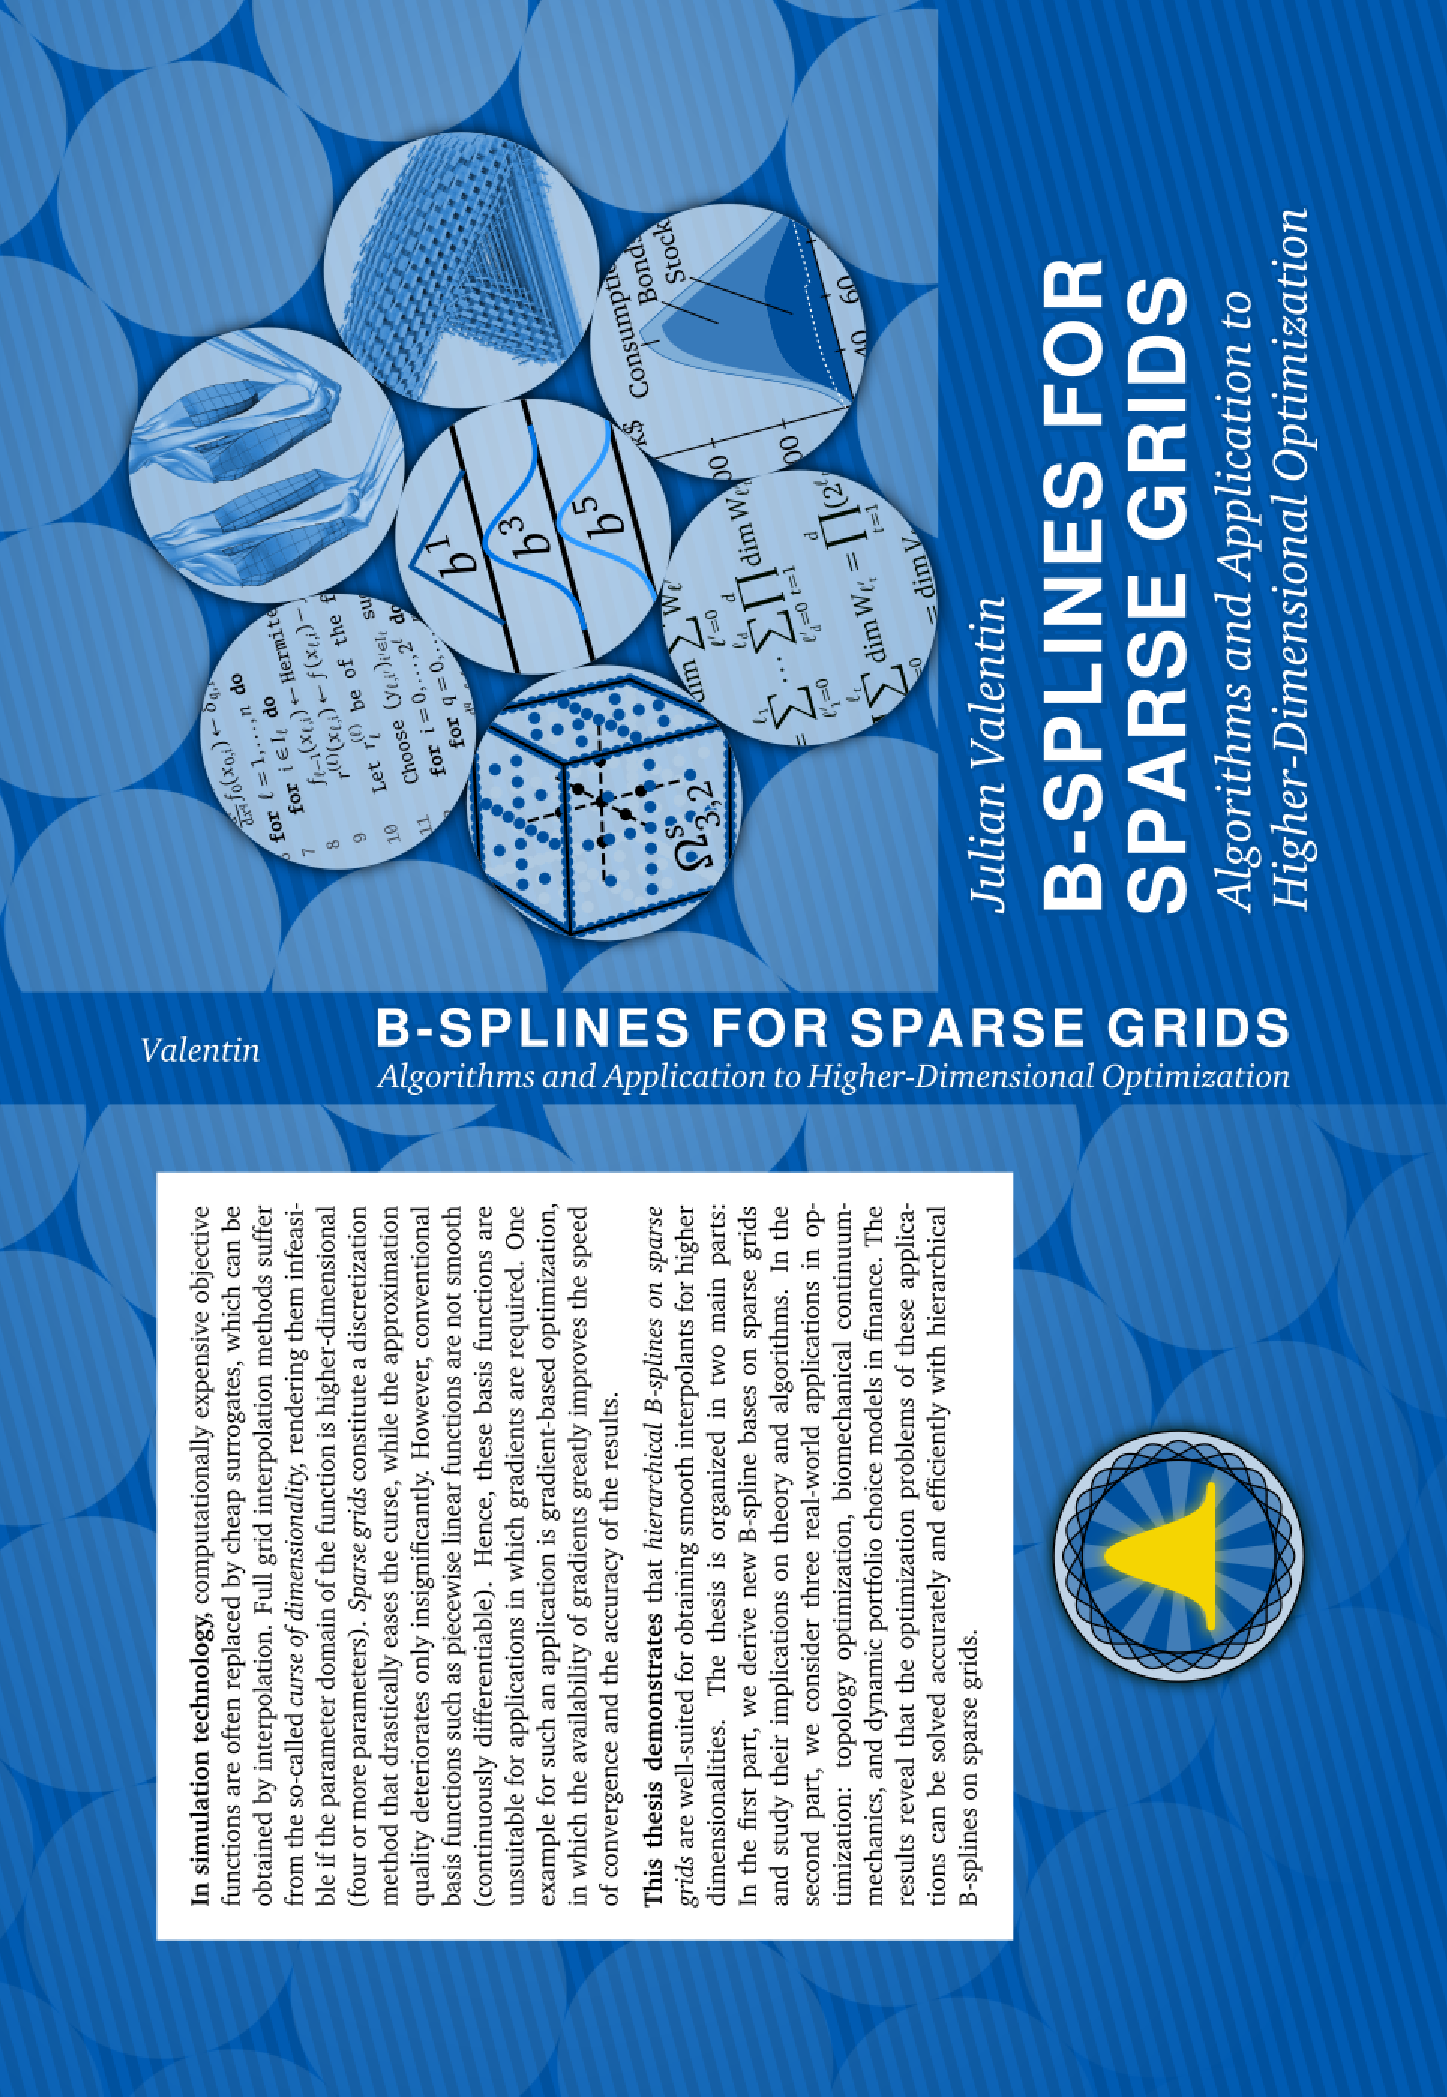
\includepdf{coverPublishedScreen}

% insert empty page
\cleardoublepage

% reset page numbering, use arabic numbers
\pagenumbering{arabic}
\setcounter{page}{1}

  
  \iftoggle{partialCompileMode}{}{
    % title page
    \begin{titlepage}
  \begin{spacing}{1}
    \begin{center}
      \begin{otherlanguage}{ngerman}
        % no indentation of paragraphs
        \setlength{\parindent}{0pt}
        
        {\bfseries\huge\thetitle\par}
        
        \vfill
        
        Vom Stuttgarter Zentrum für Simulationswissenschaften der\\
        Universität~Stuttgart zur Erlangung der Würde eines Doktors der\\
        Naturwissenschaften (Dr.~rer.~nat.) genehmigte Abhandlung
        
        \vfill
        
        Vorgelegt von
        
        {\bfseries\Large\theauthor\par}
        
        aus \thebirthplace
        
        \vfill
        
        \begin{tabular}{ll}
          Hauptberichter:&
          \theadvisor\\[0.5em]
          Mitberichter:&
          \theexamineri\\
          &\theexaminerii\\[1em]
          \multicolumn{2}{l}{%
            Tag der mündlichen Prüfung:\quad%
            \thedefensedate%
          }
        \end{tabular}
        
        \vfill
        
        \includegraphics[scale=1.1]{logoUniversityGerman}
        
        \vspace{2em}
        
        Vorgelegt an der \theuniversity
        
        \vspace{1em}
        
        \theinstitute{} der \theuniversity
        
        \vspace{1em}
        
        \theyear
      \end{otherlanguage}
    \end{center}
  \end{spacing}
\end{titlepage}

% don't display page number
\thispagestyle{empty}

{%
  % no indentation of paragraphs
  \setlength{\parindent}{0pt}%
  \small
  
  \begin{center}
    \includegraphics[scale=1.1]{logoUniversityEnglish}%
    
    \vspace{1em}
    
    Submitted to the University of Stuttgart
  \end{center}
  
  \begin{tabular}{@{}p{0.57\textwidth}@{}p{0.43\textwidth}@{}}
    \emph{Involved institutions and departments:}%
    \vspace{0.6mm}\newline%
    Cluster of Excellence in Simulation Technology%
    \vspace{0.6mm}\newline%
    Institute for Parallel and Distributed Systems%
    \vspace{0.6mm}\newline%
    Department for Simulation Software Engineering%
    \vspace{0.6mm}\newline%
    Department for Simulation of Large Systems&
    \raisebox{-0.5\height}{%
      
\includegraphics[scale=1.0]{logoSimTech}%
    }%
    \qquad%
    \raisebox{-0.5\height}{%
      \includegraphics[scale=1.2]{logoIPVS}%
    }%
    \vspace{2mm}\newline%
    \raisebox{-0.3888\height}{%
      \includegraphics[scale=1.0]{logoSSE}%
    }%
    \qquad%
    \raisebox{-0.5\height}{%
      \includegraphics[height=19mm]{logoSGS.png}%
    }
  \end{tabular}
  
  \vfill
  
  Compiled as version \texttt{v\compileCounter{}}
  on \currentTimeLong.\\
  \lefthphantom{%
    Committed as \texttt{\gitCommitHash{}}%
  }{%
    Compiled as version \texttt{v\compileCounter{}}%
  }
  on \gitCommitTimeLong.
  
  \vspace{1em}
  
  Typeset using \LaTeX{} and cover design by the author.
  
  \vspace{1em}
  
  \begin{tabular}{%
    @{}p{0.2\textwidth}@{}p{0.8\textwidth}@{}%
  }
    \includegraphics[height=10mm]{licenseBadge}&
    \raisebox{3.8mm}{%
      \parbox{\linewidth}{%
        Copyright \copyright{} \theyear{} \theauthor{}.
        This work is licensed under the
        \term{%
          \href{https://creativecommons.org/licenses/by-sa/4.0/}{%
            Creative Commons Attribution-ShareAlike 4.0
            International License%
          }%
        }.%
      }%
    }
  \end{tabular}
  
  \vspace{1em}
  
  Although this thesis was written with uttermost care,
  it cannot be ruled out that it contains errors.
  Please send any corrections and mistakes to
  \href{mailto:thesis@bsplines.org}{\texttt{thesis@bsplines.org}}.
}

\cleardoublepage

    
    % dedication
    % don't display page number
\thispagestyle{empty}

\vspace*{\fill}

\begin{center}
  \includegraphics[width=0.6\textwidth]{dedicationQuote}
  
  \begin{minipage}{0.6\textwidth}%
    \begin{flushright}
      \small--- Carl de~Boor \cite{Boor16Comment}
    \end{flushright}
  \end{minipage}
\end{center}

\vspace*{\fill}

\begin{center}
  \includegraphics{logoBSplines}%
\end{center}

\vspace*{\fill}

\cleardoublepage

  }
  
  % progress page
  \iftoggle{draftMode}{
    \begin{center}
  \textbf{Writing, Testing, and Editing Progress}
  
  \noindent\small%
  \renewcommand*{\arraystretch}{0.65}%
  \setlength{\tabcolsep}{0mm}%
  \newcommand*{\pc}[1]{%
    \textbf{\textcolor{C4!#1!C1}{#1}}%
  }%
  \newcommand*{\pr}[1]{%
    \textbf{\textcolor{C4!#1!C1}{\righthphantom{#1}{100}}}%
  }%
  \newcommand*{\thead}{
    \textbf{Sc}&
    \multicolumn{3}{c}{\hspace*{-8mm}\textbf{Writing}}&
    \multicolumn{3}{c}{\hspace*{-7mm}\textbf{Testing}}&
    \multicolumn{6}{c}{\hspace*{-5mm}\textbf{Editing}}&
    \textbf{Rem}\\
    \cmidrule(r{9mm}){2-4}
    \cmidrule(r{7mm}){5-7}
    \cmidrule(r{5mm}){8-13}
    \cmidrule(r{2mm}){14-14}
    &
    \multicolumn{2}{c}{\hspace*{-2mm}\textbf{Pages}}&\textbf{\%}&
    \multicolumn{2}{c}{\hspace*{-3mm}\textbf{Tests}}&\textbf{\%}&
    \textbf{Slf}&\textbf{Con}&\textbf{Cll}&
    \textbf{Drk}&\textbf{Fnl}&\textbf{\%}&
    \textbf{Cll}\\
    \midrule
  }%
  \luaexec{require("progressTable")}%
  \newcommand*{\tfoot}{\luadirect{generateTotalRow()}}%
  \scalebox{1.0}[1.0]{%
    \begin{tabular}{
      @{\hspace{2mm}}
      c
      @{\hspace{6mm}}
      r@{/}r@{\hspace{3mm}}r
      @{\hspace{9mm}}
      r@{/}r@{\hspace{3mm}}r
      @{\hspace{7mm}}
      *{5}{D{8mm}}
      r
      @{\hspace{5mm}}
      c
      @{\hspace{2mm}}
    }
      \toprule
      \thead 1.0 &  4 &  4 & \pr{100} &  0 &  0 & \pr{100} & \yes & \yes & \yes & \yes & \no  &  \pr{80} & T         \\ \midrule
      2.0        &  1 &  1 & \pr{100} &  0 &  0 & \pr{100} & \yes & \yes & \yes & \yes & \no  &  \pr{80} & C         \\
      2.1        &  4 &  4 & \pr{100} &  1 &  1 & \pr{100} & \yes & \yes & \yes & \no  & \no  &  \pr{60} & C         \\
      2.2        &  4 &  4 & \pr{100} &  2 &  2 & \pr{100} & \yes & \yes & \yes & \no  & \no  &  \pr{60} & C         \\
      2.3        &  5 &  5 & \pr{100} &  0 &  0 & \pr{100} & \yes & \yes & \yes & \no  & \no  &  \pr{60} & C         \\
      2.4        &  8 &  8 & \pr{100} &  5 &  5 & \pr{100} & \yes & \yes & \yes & \no  & \no  &  \pr{60} & C         \\ \midrule
      3.0        &  1 &  1 & \pr{100} &  0 &  0 & \pr{100} & \yes & \yes & \yes & \no  & \no  &  \pr{60} & H, MR, R  \\
      3.1        & 14 & 14 & \pr{100} &  5 &  5 & \pr{100} & \yes & \yes & \yes & \no  & \no  &  \pr{60} & MR        \\
      3.2        & 11 & 11 & \pr{100} &  4 &  4 & \pr{100} & \yes & \yes & \yes & \no  & \no  &  \pr{60} & MR        \\ \midrule
      4.0        &  1 &  1 & \pr{100} &  0 &  0 & \pr{100} & \yes & \yes & \yes & \no  & \no  &  \pr{60} & H, MR     \\
      4.1        &  3 &  3 & \pr{100} &  0 &  0 & \pr{100} & \yes & \yes & \yes & \no  & \no  &  \pr{60} & MR        \\
      4.2        &  3 &  3 & \pr{100} &  2 &  2 & \pr{100} & \yes & \yes & \yes & \no  & \no  &  \pr{60} & MR        \\
      4.3        &  9 &  9 & \pr{100} &  8 &  8 & \pr{100} & \yes & \yes & \yes & \no  & \no  &  \pr{60} & MR        \\
      4.4        & 17 & 17 & \pr{100} &  5 &  5 & \pr{100} & \yes & \yes & \yes & \no  & \no  &  \pr{60} & B         \\
      4.5        & 15 & 15 & \pr{100} & 10 & 10 & \pr{100} & \yes & \yes & \no  & \no  & \no  &  \pr{40} & (G)       \\ \midrule
      5.0        &  1 &  1 & \pr{100} &  0 &  0 & \pr{100} & \yes & \yes & \no  & \no  & \no  &  \pr{40} & (MB)      \\
      5.1        &  7 &  7 & \pr{100} &  0 &  0 & \pr{100} & \yes & \yes & \no  & \no  & \no  &  \pr{40} & (MB)      \\
      5.2        &  3 &  3 & \pr{100} &  0 &  0 & \pr{100} & \yes & \yes & \no  & \no  & \no  &  \pr{40} & (MB)      \\
      5.3        &  3 &  3 & \pr{100} &  0 &  0 & \pr{100} & \yes & \yes & \no  & \no  & \no  &  \pr{40} & (MB)      \\
      5.4        & 10 & 10 & \pr{100} &  0 &  0 & \pr{100} & \yes & \yes & \no  & \no  & \no  &  \pr{40} & (MB)      \\
      5.5        &  8 &  8 & \pr{100} &  0 &  0 & \pr{100} & \yes & \yes & \no  & \no  & \no  &  \pr{40} & (MB)      \\ \midrule
      6.0        &  1 &  1 & \pr{100} &  0 &  0 & \pr{100} & \yes & \no  & \no  & \no  & \no  &  \pr{20} & (T)       \\
      6.1        &  4 &  4 & \pr{100} &  0 &  0 & \pr{100} & \yes & \no  & \no  & \no  & \no  &  \pr{20} & (T)       \\
      6.2        &  5 &  5 & \pr{100} &  0 &  0 & \pr{100} & \yes & \no  & \no  & \no  & \no  &  \pr{20} & (T)       \\
      6.3        &  0 &  3 &   \pr{0} &  0 &  0 & \pr{100} & \no  & \no  & \no  & \no  & \no  &   \pr{0} & (T)       \\
      6.4        &  0 &  9 &   \pr{0} &  0 &  0 & \pr{100} & \no  & \no  & \no  & \no  & \no  &   \pr{0} & (T)       \\ \midrule
      7.0        &  1 &  1 & \pr{100} &  0 &  0 & \pr{100} & \yes & \no  & \no  & \no  & \no  &  \pr{20} & (B)       \\
      7.1        &  3 &  3 & \pr{100} &  0 &  0 & \pr{100} & \yes & \no  & \no  & \no  & \no  &  \pr{20} & (B)       \\
      7.2        &  5 &  5 & \pr{100} &  0 &  0 & \pr{100} & \yes & \no  & \no  & \no  & \no  &  \pr{20} & (B)       \\
      7.3        &  9 &  9 & \pr{100} &  0 &  0 & \pr{100} & \yes & \no  & \no  & \no  & \no  &  \pr{20} & (B)       \\ \midrule
      8.0        &  2 &  2 & \pr{100} &  0 &  0 & \pr{100} & \no  & \no  & \no  & \no  & \no  &   \pr{0} & (G)       \\
      8.1        &  4 &  4 & \pr{100} &  0 &  0 & \pr{100} & \no  & \no  & \no  & \no  & \no  &   \pr{0} & (G)       \\
      8.2        &  7 &  7 & \pr{100} &  0 &  0 & \pr{100} & \no  & \no  & \no  & \no  & \no  &   \pr{0} & (G)       \\
      8.3        &  2 &  3 &  \pr{67} &  0 &  0 & \pr{100} & \no  & \no  & \no  & \no  & \no  &   \pr{0} & (G)       \\
      8.4        &  0 &  8 &   \pr{0} &  0 &  0 & \pr{100} & \no  & \no  & \no  & \no  & \no  &   \pr{0} & (G)       \\ \midrule
      9.0        &  0 &  4 &   \pr{0} &  0 &  0 & \pr{100} & \no  & \no  & \no  & \no  & \no  &   \pr{0} & (T)       \\ \midrule
      A.0        &  0 &  0 & \pr{100} &  0 &  0 & \pr{100} & \yes & \yes & --   & \no  & \no  &  \pr{50} & --        \\
      A.1        &  3 &  3 & \pr{100} &  0 &  0 & \pr{100} & \yes & \yes & --   & \no  & \no  &  \pr{50} & --        \\
      A.2        &  2 &  2 & \pr{100} &  0 &  0 & \pr{100} & \yes & \yes & --   & \no  & \no  &  \pr{50} & --        \\
      A.3        & 15 & 15 & \pr{100} &  2 &  2 & \pr{100} & \yes & \yes & --   & \no  & \no  &  \pr{50} & --        \\ \midrule
      B.0        &  0 &  0 & \pr{100} &  0 &  0 & \pr{100} & \yes & \yes & --   & \no  & \no  &  \pr{50} & --        \\
      B.1        &  2 &  2 & \pr{100} &  0 &  0 & \pr{100} & \yes & \yes & --   & \no  & \no  &  \pr{50} & --        \\
      B.2        &  2 &  2 & \pr{100} &  0 &  0 & \pr{100} & \yes & \yes & --   & \no  & \no  &  \pr{50} & -- \tfoot \\ \bottomrule
    \end{tabular}
  }%
\end{center}

\clearpage

\noindent
\textbf{Explanation:}

\begin{itemize}
  \item
  \textbf{Sc:}
  Section
  
  \item
  \textbf{Writing/Pages:}
  As counted in the Table of Contents
  (next section minus this section)
  
  \item
  \textbf{Testing/Tests:}
  Should be one Python unit test per theorem-like statement
  
  \item
  \textbf{Editing:}
  \begin{itemize}
    \item
    \textbf{Slf:}
    First self-editing round, fix obvious errors
    
    \item
    \textbf{Con:}
    Correction of contents (statements, formulas, theorems, \dots);
    shorten text, use better language
    
    \item
    \textbf{Cll:}
    Editing by a colleague
    
    \item
    \textbf{Drk:}
    Editing by Dirk
    
    \item
    \textbf{Fnl:}
    Final proofreading, setting line/page breaks manually
  \end{itemize}
  
  \item
  \textbf{Rem:}
  Remarks
  \begin{itemize}
    \item
    \textbf{Cll:}
    Colleague(s) who read the section
    (\textbf{B}enni,
    \textbf{C}aro,
    \textbf{G}regor,
    \textbf{H}enriette,
    \textbf{M}alte \textbf{B}.,
    \textbf{M}ichael \textbf{R}.,
    \textbf{R}alf,
    \textbf{T}heresa)
  \end{itemize}
\end{itemize}

\noindent
\textbf{Feedback from colleagues to be considered:}

\begin{itemize}
  \item
  Less passive voice (H)
  
  \item
  More signposts (H)
  
  \item
  More concrete statements, less ``some'' etc. (H)
  
  \item
  Less embedded clauses, interrupts flow of reading (MR)
  
  \item
  Less ``so-called'' (MR)
\end{itemize}

\cleardoublepage

  }{}
  
  \iftoggle{partialCompileMode}{}{
    % table of contents, create bookmark
    % create PDF bookmark
\pdfbookmark[section]{\contentsname}{toc}
\tableofcontents

\cleardoublepage

    
    % lists of floats and theorems
    % ======================================================================
% Floats
% ======================================================================

% define mdframed style for floats
\mdfdefinestyle{floatmdfstyle}{
  innerleftmargin=7pt,
  innerrightmargin=7pt,
  innertopmargin=7pt,
  innerbottommargin=6pt,
  roundcorner=10pt,
  linewidth=1pt,
  linecolor=mittelblau,
  backgroundcolor=mittelblau!10,
  % the documentation of mdframed lies about the default values of
  % splittopskip and splitbottomskip
  splittopskip=15pt,
  splitbottomskip=5pt,
  % replace drop shadow with blur shadow
  shadow=true,
  apptotikzsetting={%
    % alternatively, use
    % \tikzset{mdfshadow/.style={blur shadow={shadow blur steps=5}}}%
    % from the pgf-blur package;
    % disadvantage of that is that this uses semi-transparency,
    % which some printers/printing services cannot handle
    % ==> recreate pgf-blur shadow effect with opaque drop shadows
    \tikzset{
      every shadow/.style={shadow xshift=1mm,shadow yshift=-1mm,opacity=1},
      mdfshadow/.style={
        drop shadow={line width=2.4mm,draw=black!03,fill=black!03},
        drop shadow={line width=2.1mm,draw=black!06,fill=black!06},
        drop shadow={line width=1.8mm,draw=black!09,fill=black!09},
        drop shadow={line width=1.5mm,draw=black!12,fill=black!12},
        drop shadow={line width=1.2mm,draw=black!15,fill=black!15},
        drop shadow={line width=0.9mm,draw=black!18,fill=black!18},
        drop shadow={line width=0.6mm,draw=black!21,fill=black!21},
        drop shadow={line width=0.3mm,draw=black!24,fill=black!24},
        drop shadow={draw=none,fill=black!27},
        drop shadow={draw=none,fill=black!30,
                     shadow xshift=0.85mm,shadow yshift=-0.85mm,},
        drop shadow={draw=none,fill=black!33,
                     shadow xshift=0.70mm,shadow yshift=-0.70mm,},
        drop shadow={draw=none,fill=black!36,
                     shadow xshift=0.35mm,shadow yshift=-0.35mm,},
        drop shadow={draw=none,fill=black!39,
                     shadow xshift=0.40mm,shadow yshift=-0.40mm,},
      }
    }%
  },
}

% make "tp" to default position of figure and table
\def\fps@figure{tp}
\def\fps@table{tp}

% wrap floats in mdframed boxes,
% automatically center all float contents,
% change font size in float environments
\apptocmd{\@xfloat}{\begin{mdframed}[style=floatmdfstyle]\centering\small}{}{}
\pretocmd{\end@float}{\end{mdframed}}{}{}

% make internal length of sidecap smaller to account for smaller space
% for floats with side captions
\xpatchcmd{\endSC@float}{\endSC@FLOAT\@tempdima}{%
  \setlength{\@tempdima}{\@tempdima-17pt}\endSC@FLOAT\@tempdima%
}{}{}

% automatically center all subfigure contents
\apptocmd{\subcaption@minipage}{\centering}{}{}

% don't move floats to own page (float page) when they are tall,
% the default value is 0.5, which is a bit small
\renewcommand*{\floatpagefraction}{0.7}

% space between floats and text
\setlength{\textfloatsep}{20pt}

    
    % list of symbols and acronyms
    % ======================================================================
% Glossary
% ======================================================================

% \newcommand with variable command names
\newcommand*{\newnamecommand}{\@star@or@long\new@name@command}
\newcommand*{\new@name@command}[1]{\expandafter\new@command\csname #1\endcsname}

\iftoggle{partialCompileMode}{
  % define dummy commands that work as if partialCompileMode was disabled
  \newcommand*{\newnotation}[3]{%
    \expandafter\newcommand\csname notationsymbol\string#1\endcsname{#2}%
    \expandafter\newcommand\csname notationtext\string#1\endcsname{#3}%
  }
  \newcommand*{\newnotationcommand}[6][0]{%
    \newcommand*{#2}[#1]{#3}%
    \makecommandnotation{#2}{#4}{#5}{#6}%
  }
  \newcommand*{\newnotationcommandoptarg}[7][]{%
    \newcommand*{#3}[#2][#1]{#4}%
    \makecommandnotation{#3}{#5}{#6}{#7}%
  }
  \newcommand*{\hidenextnotation}{}
  \newcommand*{\makecommandnotation}[4]{%
    \expandafter\newcommand\csname notationsymbol\string#1\endcsname{#3}%
    \expandafter\newcommand\csname notationtext\string#1\endcsname{#4}%
  }
  \newcommand*{\usenotation}[1]{\ignorespaces}
  \newcommand*{\printnotationsymbol}[1]{%
    \csname notationsymbol\string#1\endcsname%
  }
  \newcommand*{\printnotationtext}[1]{%
    \csname notationtext\string#1\endcsname%
  }
  
  \newcommand*{\newgacronym}[3][]{%
    \if\relax\detokenize{#1}\relax%
      \newnamecommand{#2}{\MakeUppercase{#2}\xspace}%
      \newnamecommand{#2s}{\MakeUppercase{#2}s\xspace}%
      \newnamecommand{#2c}{\MakeUppercase{#2}\xspace}%
      \newnamecommand{#2sc}{\MakeUppercase{#2}s\xspace}%
    \else%
      \newnamecommand{#2}{#1\xspace}%
      \newnamecommand{#2s}{#1s\xspace}%
      \newnamecommand{#2c}{\makefirstuc{#1}\xspace}%
      \newnamecommand{#2sc}{\makefirstuc{#1}s\xspace}%
    \fi%
  }
  \newcommand*{\hidegacronym}[1]{}
}{
  % define new glossary style based on long (uses longtable)
  % in which the column widths are fixed and space before/after the
  % table is removed
  \newglossarystyle{longraggedfixed}{
    % base glossary style
    \setglossarystyle{long}
    
    % custom flag to check if we're in the glossary
    \newif\ifinglossary
    
    \renewenvironment{theglossary}%
    {%
      % remove space before/after glossary
      \setlength{\LTpre}{0pt}%
      \setlength{\LTpost}{0pt}%
      %
      % set custom flag that we are now in the glossary
      \inglossarytrue%
      %
      % set font size
      \small%
      %
      % use single spacing
      \begin{spacing}{1}%
        % table header
        \begin{longtable}{@{}L{0.15\textwidth}@{}L{0.85\textwidth}@{}}%
          \textbf{Symbol}\vspace{2mm}&%
          \textbf{Meaning\hfill{}Page with First Occurrence}\vspace{2mm}%
          \endhead%
    }%
    {%
      % table footer
        \end{longtable}%
      \end{spacing}%
      % set custom flag that we are now outside the glossary
      \inglossaryfalse%
    }
  
    % add dotted leaders between entry description and page number
    % (called for every row of the table)
    \renewcommand*{\glossentry}[2]{%
      \glsentryitem{##1}\glstarget{##1}{\glossentryname{##1}}&%
      \glossentrydesc{##1}\leavevmode\kern3pt\leaders\hbox{%
        \hspace{0.2237em}.\hspace{0.2237em}%
      }\hfill\kern0pt%
      ##2%
      \tabularnewline%
    }
  }
  
  % use new glossary style
  \setglossarystyle{longraggedfixed}
  
  % add field to glossary entries that stores whether the entry
  % has been used at least once in the document
  \glsaddstoragekey{myused}{false}{\glsmyused}
  \glsaddstoragekey{myisacronym}{false}{\glsmyisacronym}
  
  % \newnotation{sortKey}{entrySymbol}{entryText}
  % adds notation to the glossary without command,
  % only to be used with \usenotation
  \newcommand*{\newnotation}[3]{%
    \newglossaryentry{#1}{text={},sort={#1},name={#2},description={#3}}%
    \expandafter\newcommand\csname notationsymbol\string#1\endcsname{#2}%
    \expandafter\newcommand\csname notationtext\string#1\endcsname{#3}%
  }
  
  % \newnotationcommand[numberOfArgs]{\commandName}
  %   {commandDefinition}{sortKey}{entrySymbol}{entryText}
  % adds notation to the glossary and creates a command
  \newcommand*{\newnotationcommand}[6][0]{%
    \newcommand*{#2}[#1]{#3}%
    \makecommandnotation{#2}{#4}{#5}{#6}%
  }
  
  % \newnotationcommandoptarg[defaultValue]{numberOfArgs}{\commandName}
  %   {commandDefinition}{sortKey}{entrySymbol}{entryText}
  % is like \newnotationcommand, but with an optional argument for
  % the command to be created
  \newcommand*{\newnotationcommandoptarg}[7][]{%
    \newcommand*{#3}[#2][#1]{#4}%
    \makecommandnotation{#3}{#5}{#6}{#7}%
  }
  
  % custom flag to hide the entry defined by the next \newnotationcommand
  % (or similar) from the glossary
  \newif\ifhidenextnotation
  \newcommand*{\hidenextnotation}{\hidenextnotationtrue}
  
  % \makecommandnotation{\commandName}{sortKey}{entrySymbol}{entryText}
  % adds notation to the glossary and modifies \commandName such that
  % the glossary entry is referenced on every use of \commandName
  % (except if used in the glossary itself)
  \newcommand*{\makecommandnotation}[4]{%
    \newglossaryentry{#2}{text={},sort={#2},name={#3},description={#4}}%
    \expandafter\newcommand\csname notationsymbol\string#1\endcsname{#3}%
    \expandafter\newcommand\csname notationtext\string#1\endcsname{#4}%
    \ifhidenextnotation%
      \hidenextnotationfalse%
      \pretocmd{#1}{\glsfieldgdef{#2}{myused}{true}}{}{}%
    \else%
      % only reference entry if outside glossary
      % (otherwise, the page number of the glossary would be displayed)
      \pretocmd{#1}{\ifinglossary\else\usenotation{#2}\fi}{}{}%
    \fi%
  }
  
  % \usenotation{sortKey}
  % explicitly "uses" the notation given by sortKey without printing anything
  \newcommand*{\usenotation}[1]{%
    \glsfieldgdef{#1}{myused}{true}%
    \glsdisp{#1}{\relax}\ignorespaces%
  }
  
  % \printnotationsymbol{\commandName}
  % \printnotationtext{\commandName}
  % print the symbol and the text of the notation given by \commandName
  % if the symbol was created with \makecommandnotation
  % (i.e., \newnotationcommand or \newnotationcommandoptarg);
  % if it was created with \newnotation, use sortKey as argument
  % for \printnotationsymbol and \printnotationtext
  \newcommand*{\printnotationsymbol}[1]{%
    \csname notationsymbol\string#1\endcsname%
  }
  \newcommand*{\printnotationtext}[1]{%
    \csname notationtext\string#1\endcsname%
  }
  
  % shortcut for \newacronym, automatically generating
  % a corresponding shortcut for \gls
  \newcommand*{\newgacronym}[3][]{%
    \if\relax\detokenize{#1}\relax%
      \newacronym[sort={Ü#2},description={\makefirstuc{#3}}]%
      {Ü#2}{\MakeUppercase{#2}}{#3}%
    \else%
      \newacronym[sort={Ü#2},description={\makefirstuc{#3}}]{Ü#2}{#1}{#3}%
    \fi%
    \glsfieldgdef{Ü#2}{myisacronym}{true}%
    \newnamecommand{#2}{\glsfieldgdef{Ü#2}{myused}{true}\gls{Ü#2}\xspace}%
    \newnamecommand{#2s}{\glsfieldgdef{Ü#2}{myused}{true}\glspl{Ü#2}\xspace}%
    \newnamecommand{#2c}{\glsfieldgdef{Ü#2}{myused}{true}\Gls{Ü#2}\xspace}%
    \newnamecommand{#2sc}{\glsfieldgdef{Ü#2}{myused}{true}\Glspl{Ü#2}\xspace}%
  }
  
  % hide specific acronyms (that are only used once) in glossary
  \newignoredglossary{hidden}
  \newcommand*{\hidegacronym}[1]{\glsmoveentry{Ü#1}{hidden}}
  
  % spell out acronyms at beginning of chapters
  \newcommand*{\resetacronyms}{%
    \forglsentries{\mysymbolname}{%
      \ifthenelse{\equal{\glsmyisacronym{\mysymbolname}}{true}}{%
        \glsreset{\mysymbolname}%
      }{}%
    }%
  }
  
  \addtokomafont{chapter}{\resetacronyms}
  
  % warn for every symbol that has not been used
  \AtEndDocument{%
    \forglsentries{\mysymbolname}{%
      \ifthenelse{\equal{\glsmyused{\mysymbolname}}{false}}{%
        \GenericWarning{}{%
          LaTeX Warning: Symbol ``\mysymbolname'' defined, but unused%
        }%
      }{}%
    }%
  }
  
  % generate table of symbols and acronyms
  \makeglossaries
}

% add debug info about definitions of glossary entries
\iftoggle{showGlossaryDefinitionsMode}{
  \let\oldnewgsymbol\newgsymbol
  \renewcommand*{\newgsymbol}[3]{%
    \ifx\@onlypreamble\@notprerr%
      \textcolor{C1}{Defining ``#2'' as ``#3''. }%
    \fi%
    \oldnewgsymbol{#1}{#2}{#3}%
  }
}{}

    
    % abstract
    \addchap{Abstract/\foreignlanguage{ngerman}{Kurzzusammenfassung}}

\printornamentsfalse

\section*{Abstract}

In simulation technology, computationally expensive objective functions
are often replaced by cheap surrogates,
which can be obtained by interpolation.
Full grid interpolation methods suffer from the
so-called curse of dimensionality,
rendering them infeasible if the parameter domain of the function
is higher-dimensional (four or more parameters).
Sparse grids constitute a discretization method that does not suffer from the
curse, while the approximation quality deteriorates only insignificantly.
However, conventional basis functions such as piecewise linear functions
are not smooth (continuously differentiable).
Hence, these basis functions are unsuitable for applications
in which gradients are required.
One example for such an application is gradient-based optimization,
in which the availability of gradients greatly improves the speed of
convergence and the accuracy of results.

This thesis demonstrates that hierarchical B-splines on sparse grids are
well-suited for obtaining smooth interpolants for higher dimensionalities.
The thesis is organized in two main parts:
In the first part, we derive new B-spline bases on sparse grids and study
their implications on theory and algorithms.
In the second part, we consider three real-world applications in optimization:
topology optimization, biomechanical continuum-mechanics, and
dynamic portfolio choice models in finance.
The results reveal that the optimization problems of these applications
can be solved accurately and efficiently with hierarchical B-splines on
sparse grids.
% 209 words

\newpage

\begin{otherlanguage}{ngerman}
  \section*{Kurzzusammenfassung}
  
  In der Simulationstechnologie werden zeitaufwendige Zielfunktionen
  oft durch einfache Surrogate ersetzt, die durch Interpolation
  gewonnen werden können.
  Vollgitter-Interpolationsmethoden leiden unter dem
  sogenannten Fluch der Dimensionalität,
  der sie unbrauchbar macht, falls der Parameterbereich der Funktion
  höherdimensional ist (vier oder mehr Parameter).
  Dünne Gitter sind eine Diskretisierungsmethode, die nicht unter
  dem Fluch leidet, aber die Approximationsqualität nur leicht verschlechtert.
  Leider sind konventionelle Basisfunktionen wie die stückweise
  lineare Funktionen nicht glatt (stetig differenzierbar).
  Daher sind sie für Anwendungen ungeeignet, in denen Gradienten
  benötigt werden.
  Ein Beispiel für eine solche Anwendung ist gradientenbasierte Optimierung,
  in der die Verfügbarkeit von Gradienten die Konvergenzgeschwindigkeit und
  die Ergebnisgenauigkeit deutlich verbessert.
  
  Diese Dissertation demonstriert, dass hierarchische B-Splines auf
  dünnen Gittern gut geeignet sind,
  um glatte Interpolierende für höhere Dimensionalitäten zu erhalten.
  Die Dissertation ist in zwei Hauptbereiche gegliedert:
  Der erste Teil leitet neue B-Spline-Basen auf dünnen Gittern her und
  untersucht ihre Implikationen bezüglich Theorie und Algorithmen.
  Der zweite Teil behandelt drei Realwelt-Anwendungen aus der Optimierung:
  Topologieoptimierung, biomechanische Kontinuumsmechanik und
  Modelle der dynamischen Portfolio-Wahl in der Finanzmathematik.
  Die Ergebnisse zeigen, dass die Optimierungsprobleme dieser
  Anwendungen durch hierarchische B-Splines auf dünnen Gittern
  genau und effizient gelöst werden können.
  % 188 Wörter
\end{otherlanguage}

\printornamentstrue
\cleardoublepage

    
    % preface
    \addchap{Preface}

Before I start, I want to thank my advisor Prof.\ Dr.\ Dirk Pflüger.
It is his ideas and his valuable input that have driven me in
my time as a PhD student.
I am also grateful for the exciting time with the whole group of
SSE (Simulation Software Engineering) and
SGS (Simulation of Large Systems),
for which I want to thank all past and current PhD students and postdocs of
Dirk Pflüger and Prof.\ Dr.\ Miriam Mehl.
I thank
Carolin Schober,
Henriette Röger, and
Ralf Diestelkämper
for throughly proofreading
drafts of this thesis.

Similarly, I thank my co-advisor Prof.\ Oliver Röhrle, PhD, for the
interesting biomechanical collaboration and his willingness to be my co-advisor.
Many thanks go to the other members of the examination board for their
willingness to examine my thesis,
namely \todo{insert co-examiner} and \todo{insert co-examiner}.

Probably the most important role for the success of my PhD thesis
has played my family.
Without their mental support and distraction from the daily work,
I doubt that this thesis would have been possible.

Likewise, I am very grateful for the financial support from
the \foreignlanguage{ngerman}{Juniorprofessurenprogramm} of the
\foreignlanguage{ngerman}{Landesstiftung Baden-Württemberg}.
I thank the SimTech Cluster of Excellence for supporting
my three-month research stay in Canberra, Australia.

In addition, I want to thank the open-source community for making it possible to
write this thesis in an aesthetically sophisticated manner.
The list of software that was used to write this thesis includes
\LaTeX, Lua\LaTeX, Bib\LaTeX,
\scalebox{0.9}{\KOMAScript}, Ti\emph{k}Z, Python, Matplotlib,
and many more.

\label{page:preface}
Now, I wish that you, dear reader, obtain as much insight as possible
while reading the remaining
\pagedifference{page:preface}{LastPage} pages of this thesis.

Enjoy!

\vspace{1em}

\noindent
Stuttgart, \thedate

\noindent
\theauthor

  }
  
  % chapters
  \setdictum{%
  There is a fine line between wrong and visionary.
  Unfortunately, you have to be a visionary to see it\dots%
}{%
  Sheldon Cooper%
}

\chapter{Introduction}

% https://visca.com/regexdict/
\lettrine{B}{-splines} (or by, between, beside)
\blindtext{}

\paragraph{Motivation}

\blindtext{}

\paragraph{Related Work}

\blindtext{}

\paragraph{Original contribution}

This thesis is written to be largely self-contained.
Therefore, it is necessary that some introductory definitions and
results are repeated from the literature,
which is properly attributed in the respective chapters.
In addition, some new results have already been published in accordance
with the regulations for PhD theses at the University of Stuttgart.
Whenever a publication of the author of this thesis and his supervisor
is co-authored by collaborators,
the original contribution of the author is highlighted 
at the beginning of the respective chapters or sections.

\paragraph{Notation}

The notation of this thesis tries to be intuitive and suggestive.
For example, vectors are written in bold face, which allows for
very similar formulas for the univariate and the multivariate case
(e.g., $\sum_{l'=0}^l \sum_{i' \in \hiset{l'}}
\surplus{l',i'} \basis{l',i'}$ becomes
$\sum_{\ßl'=\ß0}^\ßl \sum_{\ßi' \in \hiset{\ßl'}}
\surplus{\ßl',\ßi'} \basis{\ßl',\ßi'}$).
Other necessary notation is introduced in the text when needed.
If a symbol or an abbreviation is unclear,
it is likely explained in the glossary at the beginning of the thesis.

\paragraph{Outline}

\blindtext{}

\cleardoublepage

  \setdictum{%
  To avoid the curse of dimensionality
  we introduced regular sparse grids based on piecewise linear B-splines.%
}{%
  Bastian Bohn and Michael Griebel \cite{Bohn13Adaptive}%
}

\chapter{Sparse Grids with Arbitrary Tensor Product Bases}
\label{chap:20sparseGrids}

\todo{Write short intro to SGs? Overlap with Chap. 1?}

This chapter provides a consistent notational framework
for the definition of sparse grids with general basis functions.
The reason not to employ specific bases such as the common hat functions
or B-splines of higher degrees is two-fold:
First, we will define various new ``flavors'' of B-splines,
which is easier if the basis is left open.
Second, most of the statements and theorems that we will make in this
thesis will hold for general basis functions
(in some cases with additional assumptions)
and not just for B-splines.

Besides the derivation of sparse grids with
coarser boundary points in \cref{sec:24boundary},
this section is mainly
a repetition of the definition of sparse grids with general basis functions.
Our notation and presentation will follow roughly
\cite{Pflueger10Spatially} and \cite{Garcke13Sparse}.
A more detailed introduction to sparse grids can be found in
\cite{Bungartz04Sparse}.



\section{Nodal Basis and Nodal Space}
\label{sec:21nodalSpaces}



\subsection{Univariate Case}
\label{sec:211nodalUV}

\paragraph{Grid and basis functions}

Let us first consider univariate functions
that are defined on the unit interval $[0, 1]$.
\usenotation{l}
We discretize this domain by splitting it into $2^l$ equally sized segments,
where $l \in \NNz$ is the \term{level}.
\usenotation{i}
The resulting $2^l + 1$ \term{grid points} $\gp{l,i}$ are given by
\begin{equation}
  \gp{l,i} := i \cdot \ms{l},\quad
  i = 0, \dotsc, 2^l,
\end{equation}
where $i$ is the \term{index} and $\ms{l} := 2^{-l}$ is the \term{mesh size}.%
\footnote{%
  Note that from a strict formal perspective,
  this equation defined $\gp{l,i}$ only for $i = 0, \dotsc, 2^l$,
  but we will later need $\gp{l,i}$ also for $i < 0$ or $i > 2^l$.
  The convention in this thesis is that all definitions are
  implicitly generalized whenever needed.%
}
Every grid point is associated with a \term{basis function}
\begin{equation}
  \basis{l,i}\colon [0, 1] \to \RR.
\end{equation}
In this thesis, we assume $\basis{l,i}$ to be arbitrary,
satisfying required assumptions when needed and stated.
However, it helps for both the theory and the intuition to have a
specific example of basis functions in mind.
\newgsymbol{.1}{$\cdot^1$}{%
  Superscript for ``Piecewise linear
  (basis function/function space/interpolant)%
}%
The so-called \term{hat functions} (linear B-splines), which are defined as
\begin{equation}
  \label{eq:hatFunctionUV}
  \basis{l,i}^1(x)
  := \max(1 - |\tfrac{x}{\ms{l}} - i|, 0),
\end{equation}
are the most common choice for $\basis{l,i}$.
Here and in the following,
the superscript ``1'' is the degree of the linear B-spline and
is not to be read as an exponent.
We generalize this notation to B-splines $\basis{l,i}^p$ of
arbitrary degrees $p$ in \cref{chap:30BSplines}.

\paragraph{Nodal space}

\newgsymbol{Vl}{$V_l$}{Nodal space of level $l$}%
\newgsymbol{span}{$\spn$}{Linear span (set of all linear combinations)}%
The \emph{nodal space} $V_l$ of level $l$
is defined as the linear span of all basis functions
$\basis{l,i}$:
\begin{equation}
  V_l := \spn\{\basis{l,i} \mid i = 0, \dotsc, 2^l\}.
\end{equation}
We assume that the functions $\basis{l,i}$ form a basis of $V_l$, i.e.,
every linear combination of these functions is unique.
\newgsymbol{fl}{$f_l$}{Interpolant of $f$ in $V_l$}%
\newgsymbol{ci}{$c_i$}{Coefficients of a linear combination}%
This ensures that for every objective function $f\colon [0, 1] \to \RR$,
there is a unique function $f_l\colon [0, 1] \to \RR$ such that
\begin{equation}
  \label{eq:interpFullGridUV}
  f_l
  = \sum_{i=0}^{2^l} c_i \basis{l,i},\quad
  \fa{i = 0, \dotsc, 2^l}{f_l(\gp{l,i}) = f(\gp{l,i})},
\end{equation}
for some $c_i \in \RR$.
In this case, $f_l$ is called \term{interpolant} of $f$ in $V_l$.
The nodal space $V_l^1$ is defined analogously as the span of the
hat functions $\basis{l,i}^1$.
It is the space of all linear splines,
that is, the space of all continuous functions on $[0, 1]$ that are
piecewise linear polynomials on $[\gp{l,i}, \gp{l,i+1}]$ for
$i = 0, \dotsc, 2^l - 1$ \cite{Hoellig13Approximation}.
The nodal hat function basis of level~$l = 3$
and a linear combination are shown in \cref{fig:nodalHat}.

\begin{figure}
  \subcaptionbox{%
    Basis functions $\basis{l,i}^1$ ($i = 0, \dotsc, 2^l$)
    and grid points $\gp{l,i}$ \emph{(dots)}.%
  }[75mm]{%
    \includegraphics{nodalHat_1}%
  }%
  \hfill%
  \subcaptionbox{%
    Piecewise linear interpolant $f_l^1$ as a weighted sum
    of the nodal hat functions.%
  }[75mm]{%
    \includegraphics{nodalHat_2}%
  }%
  \caption{Univariate nodal hat functions of level $l = 3$.}
  \label{fig:nodalHat}
\end{figure}



\subsection{Multivariate Case}
\label{sec:212nodalMV}

\paragraph{Cartesian and tensor products}

\newgsymbol{d}{$d$}{Dimensionality $\in \NN$}%
For the multivariate case with $d \in \NN$ dimensions,
we proceed with the usual tensor product approach,
for which we replace all indices, points, and functions with
multi-indices, Cartesian products, and tensor products, respectively.
\newgsymbol{0!}{$\ß0$}{$(0, \dotsc, 0) \in \NNz^d$}%
\newgsymbol{1!}{$\ß1$}{$(1, \dotsc, 1) \in \NN^d$}%
\newgsymbol{01!c}{$[\ß0, \ß1]$}{%
  Unit hypercube $:= [0, 1]^d := \{x \in \RR \mid 0 \le x \le 1\}^d$%
}
\newgsymbol{l!}{$\ßl$}{Multivariate level $\in \NNz^d$}%
\newgsymbol{||.||1}{$\norm{\cdot}_1$}{%
  $\ell_1$ norm $\norm{\ßx}_1 := \sum_{t=1}^d x_t$%
}%
Therefore, the domain is now $[\ß0, \ß1] := [0, 1]^d$,
which can be partitioned into
$\prod_{t=1}^d 2^{l_t} = 2^{\norm{\vec{l}}_1}$ equally sized hypercubes,
where $\ßl = (l_1, \dotsc, l_d) \in \NNz^d$ is the $d$-dimensional level
and $\norm{\vec{l}}_1 := \sum_{t=1}^d l_t$ is the level sum.
\newgsymbol{i!}{$\ßi$}{Multivariate index $= \ß0, \dotsc, \ß2^\ßl$}%
\newgsymbol{i02l!}{$\ßi = \ß0, \dotsc, \ß2^\ßl$}{%
  For all $\ßi$ with $0 \le i_t \le 2^{l_t}$ for all $t = 1, \dotsc, d$%
}%
The corners of the hypercubes are given by the grid points
\begin{equation}
  \label{eq:gridPointMultivariate}
  \vgp{\ßl,\ßi} := \ßi \cdot \vms{ßl},\quad
  \ßi = \ß0, \dotsc, \ß2^{\ßl}.
\end{equation}
To allow for a somewhat intuitive and suggestive notation,
relations and operations with vectors (in bold face)
are to be read coordinate-wise in this thesis, unless stated otherwise.
Bold-faced numbers like $\ß0$ are defined to be the vector $(0, \dotsc, 0)$
in which every entry is equal to that number.
For example, \eqref{eq:gridPointMultivariate} is equivalent to
\begin{equation}
  \vgp{\ßl,\ßi}
  := (i_1 \ms{l_1},\; \dotsc,\; i_d \ms{l_d}),\quad
  i_t = 0, \dotsc, 2^{l_t},\quad
  t = 1, \dotsc, d,
\end{equation}
with the $d$-dimensional mesh size
$\vms{ßl} := \ß2^{-\ßl} = (\ms{l_1}, \dotsc, \ms{l_d})$.
\newgsymbol{phili!}{$\basis{\ßl,\ßi}$}{%
  Multivariate hierarchical basis function of level $\ßl$, index $\ßi$%
}%
Again, every grid point is associated with a basis function that is defined
as the tensor product of the univariate functions:%
\footnote{%
  Note that one could employ basis functions of different types in
  each dimension, for example B-splines of different degrees.
  For simplicity, we first restrict ourselves to the case of a single type
  for all dimensions, but we will treat the more general case in
  \todo{insert reference}.%
}
\begin{equation}
  \basis{\ßl,\ßi}\colon [\ß0, \ß1] \to \RR,\quad
  \basis{\ßl,\ßi}(\ßx)
  := \prod_{t=1}^d \basis{l_t,i_t}(x_t).
\end{equation}
\cref{fig:nodalHat2D} shows an example of a bivariate nodal hat function
$\basis{\ßl,\ßi}^1$.

\begin{SCfigure}
  \includegraphics{nodalHat2D_1}%
  \caption{%
    Bivariate nodal hat function of level $\ßl = (2, 1)$ and
    index $i = (1, 1)$ as the tensor product of two univariate
    nodal hat functions.%
  }%
  \label{fig:nodalHat2D}%
\end{SCfigure}

\paragraph{Multivariate nodal space}

\newgsymbol{Vl!}{$V_\ßl$}{Multivariate nodal space of level $\ßl$}%
The multivariate nodal space $V_\ßl$ is defined analogously to
the univariate case:
\begin{equation}
  V_\ßl
  := \spn\{\basis{\ßl,\ßi} \mid \ßi = \ß0, \dotsc, \ß2^{\ßl}\}.
\end{equation}
\newgsymbol{ab!}{$[\ßa, \ßb]$}{%
  Hypercube $:= [a_1, b_1] \times \dotsb \times [a_d, b_d]$%
}%
In the case of hat functions $\basis{\ßl,\ßi}^1$,
the nodal space $V_\ßl^1$ is the $d$-linear spline space
\cite{Hoellig13Approximation}, i.e.,
the space of all continuous functions
on $[\ß0, \ß1]$ that are piecewise $d$-linear polynomials on
all hypercubes
\begin{equation}
  [\vgp{\ßl,\ßi}, \vgp{\ßl,\ßi+\ß1}]
  := [\gp{l_1,i_1}, \gp{l_1,i_1+1}] \times \dotsb \times
  [\gp{l_d,i_d}, \gp{l_d,i_d+1}],\quad
  \ßi = \ß0, \dotsc, \ß2^\ßl - \ß1.
\end{equation}
\newgsymbol{fl!}{$f_\ßl$}{Interpolant of $f$ in $V_\ßl$}%
\newgsymbol{ci!}{$c_\ßi$}{Coefficients of a linear combination}%
Analogously to \eqref{eq:interpFullGridUV},
we can interpolate objective functions $f\colon [\ß0, \ß1] \to \RR$
in the nodal space $V_\ßl$ with $f_\ßl\colon [\ß0, \ß1] \to \RR$ satisfying
\begin{equation}
  \label{eq:interpFullGridMV}
  f_\ßl
  = \sum_{\ßi=\ß0}^{\ß2^\ßl} c_\ßi \basis{\ßl,\ßi},\quad
  \fa{\ßi = \ß0, \dotsc, \ß2^\ßl}{f_\ßl(\vgp{\ßl,\ßi}) = f(\vgp{\ßl,\ßi})},
\end{equation}
where $c_\ßi \in \RR$ and
the sum is over all $\ßi = \ß0, \dotsc, \ß2^\ßl$.
\begin{lemma}[linear independence of tensor products]
  \label{lemma:tensorProductLinearIndependence}
  The functions $\basis{\ßl,\ßi}$ ($\ßi = \ß0, \dotsc, \ß2^\ßl$)
  form a basis of $V_\ßl$, if the univariate functions
  $\basis{l_t,i_t}$ ($i_t = 0, \dotsc, 2^{l_t}$)
  form a basis of the univariate nodal space $V_{l_t}$
  for $t = 1, \dotsc, d$.
\end{lemma}
\begin{proof}
  \newgsymbol{!equiv}{$\equiv$}{%
    Equality of functions everywhere on their domain
    (e.g., $f \equiv 0$ means $f(x) = 0$ for all feasible $x$)%
  }%
  Assume that $c_\ßi \in \RR$ are chosen in \eqref{eq:interpFullGridMV}
  such that $f_\ßl \equiv 0$.
  Then for all $\ßi' = \ß0, \dotsc, \ß2^\ßl$,
  we can evaluate \eqref{eq:interpFullGridMV} at $\vgp{\ßl,\ßi'}$ to obtain
  \begin{equation}
    \sum_{i_1=0}^{2^{l_1}}
    \left(\sum_{i_2=0}^{2^{l_2}} \dotsb
    \left(\sum_{i_d=0}^{2^{l_d}} c_\ßi \basis{l_d,i_d}(\gp{l_d,i_d'})\right) \dotsb
    \basis{l_2,i_2}(\gp{l_2,i_2'})\right) \basis{l_1,i_1}(\gp{l_1,i_1'})
    = 0.
  \end{equation}
  We apply the linear independence in 1D ($x_1$ direction) to conclude that
  the sum over $i_2$ must vanish.
  Repeating this argument for all dimensions, we infer that $c_\ßi = 0$
  for all~$\ßi = \ß0, \dotsc, \ß2^\ßl$,
  implying the linear independence of the functions $\basis{\ßl,\ßi}$.
\end{proof}
\newgsymbol{Omegal!}{$\Omega_\ßl$}{Set of full grid points of level $\ßl$}%
The lemma is equivalent to the statement that the coefficients $c_\ßi \in \RR$
exist for every objective function $f$ and are uniquely determined by
the values at the grid points
\begin{equation}
  \Omega_\ßl
  := \{\vgp{\ßl,\ßi} \mid \ßi = \ß0, \dotsc, \ß2^{\ßl}\}.
\end{equation}
\newgsymbol{n}{$n$}{Level $\in \NNz$ of full or sparse grid}%
A common choice for the level $\ßl$ is $n \cdot \ß1$ for some $n \in \NNz$.
\newgsymbol{Vnd}{$V_{n,d}$}{%
  Multivariate nodal space
  $:= V_{n \cdot \ß1}$ of level $n$ with dimensionality $d$%
}%
In this case, we replace ``$\ßl$'' in the subscripts with ``$n{,}d$''
(for example, $V_{n,d} := V_{n \cdot \ß1}$).
\newgsymbol{||.||L2}{$\norm{\cdot}_{L^2}$}{%
  $L^2$ norm $\norm{f}_{L^2} := \sqrt{\int_\Omega f(x)^2 \dx}$
  of a function $f\colon \Omega \to \RR$%
}%
\newgsymbol{O}{$\calO(f(x))$}{Big-$\calO$ Landau notation}%
For the hat function basis $\basis{l,i}^1$,
it can be shown that the $L^2$ interpolation error of the interpolant
$f_{n,d}^1$ is given by
\begin{equation}
  \norm{f - f_{n,d}^1}_{L^2} = \calO(\ms{n}^2),
\end{equation}
i.e., the order of the interpolation error is quadratic in the mesh size
\multicite{Hoellig13Approximation,Bungartz04Sparse}.

\section{Hierarchical Basis and Hierarchical Subspace}
\label{sec:22hierSubspaces}

\newgsymbol{dim}{$\dim$}{Vector space dimension}%
\newgsymbol{|.|}{$|\cdot|$}{%
  Absolute value of a scalar or the number of elements of a set%
}%
The dimension of the nodal space $V_\ßl$ is given by
\begin{equation}
  \label{eq:dimensionFG}
  \dim V_\ßl
  = |\Omega_\ßl|
  = \prod_{t=1}^d (2^{l_t} + 1).
\end{equation}
If we choose the same level $n \in \NN_0$ in all dimensions,
then the dimension of $V_{n,d}$ and the
number of grid points grow at least as fast as
$2^{nd} = (h_n^{-1})^d$.
This exponential dependency between $\dim V_{n,d}$ and $d$ is known as the
\term{curse of dimensionality} \cite{Bungartz04Sparse,Pflueger10Spatially}.
The curse makes interpolation on $V_\ßl$ computationally infeasible
for dimensionalities $d > 4$,
as we would have to calculate and store $\dim V_\ßl$ coefficients $c_\ßi$.%
%\footnote{%
%  The number of necessary basis evaluations to evaluate the interpolant once
%  would not be as large, as most types of basis functions
%  (like hat functions $\varphi_{l,i}^1$ and higher-order B-splines)
%  are locally supported.%
%}

\subsection{Hierarchical Splitting in the Univariate Case}

\paragraph{Hierarchical subspaces}

In order to reduce the computational effort,
we first split $V_\ßl$ into smaller subspaces and then identify
which subspaces are most important and which subspaces can be omitted
at the cost of a slightly larger error.
In the univariate case, the key observation is that a grid point of a level $l$
can be written as a grid point of a higher level~$l'$:
\begin{equation}
  \label{eq:rewriteGridPoint}
  x_{l,i} = x_{l',i'},\quad
  l' \ge l,\quad
  i' = 2^{l'-l} i.
\end{equation}
\newgsymbol{xor}{$\xor$}{Bitwise ``exclusive or''}%
Conversely, this implies that every grid point $x_{l,i}$ of level $l \ge 1$
and index $i \ge 1$ can be uniquely written
as a grid point of a coarser level $l'$ and an odd index $i'$:
\begin{equation}
  x_{l,i} = x_{l',i'},\quad
  l' = l - \left[\log_2(\xor(i, i-1) + 1) - 1\right],\quad
  i' = i/2^{l-l'},
\end{equation}
% https://mathoverflow.net/a/29973
where $\xor$ is the bitwise ``exclusive or'' function.
The term in square brackets is the exponent of the
highest power of two that divides $i$.
\newgsymbol{u!}{$\dotcup$}{%
  Disjoint union of sets (union where the pairwise intersection of
  the joined sets is empty)%
}%
\newgsymbol{Il}{$I_l$}{Set of (odd) indices for hierarchical basis functions}%
As shown in \cref{fig:pointSplittingUniform},
this implies that $\Omega_l$ decomposes into
\begin{equation}
  \Omega_l
  = \bigdotcup_{l'=0}^l \{x_{l',i'} \mid i' \in I_{l'}\},\quad
  I_{l'} :=
  \begin{cases}
    \{i' = 0, \dotsc, 2^{l'} \mid \text{$i'$ odd}\},&l' > 0,\\
    \{0, 1\},&l' = 0,
  \end{cases}
\end{equation}
where $\dotcup$ indicates the disjoint union.
\newgsymbol{Wl}{$W_l$}{Hierarchical subspace of level $l$}%
We call the spaces spanned by the basis functions that correspond to the
joined sets \term{hierarchical subspaces} $W_l$:
\begin{equation}
  W_l
  := \spn\{\varphi_{l,i} \mid i \in I_l\}.
\end{equation}

\begin{figure}
  \includegraphics{pointSplitting_1}%
  \caption{%
    The set of grid points $\Omega_l$ of level $l = 4$ \emph{(top)}
    decomposes into hierarchical grids of level $l' \le l$,
    whose grid points $x_{l',i'}$ have odd indices $i' \in I_{l'}$
    ($x_{0,0}$ being the only exception).%
  }
  \label{fig:pointSplittingUniform}
\end{figure}

\paragraph{Hierarchical splitting}

\newgsymbol{oplus}{$\oplus$}{%
  Direct sum of vector spaces (vector space sum in which the dimension of
  the sum equals the sum of the summands' dimensions)%
}%
For the hat function basis $\varphi_{l,i}^1$ and other basis types,
we can prove that the corresponding nodal space
decomposes into the direct sum of all
hierarchical subspaces of coarser levels or the same level, i.e.,
\begin{equation}
  \label{eq:hierSplittingUV}
  V_l
  \overset{?}{=} \bigoplus_{l'=0}^l W_{l'},
\end{equation}
We call this relation \term{hierarchical splitting}.
Here, the direct sum $\oplus$ is
the normal vector space sum with the additional indication
that the dimension of the sum $\sum_{l'=0}^l W_{l'}$ is the sum
of the dimensions of the summands $W_{l'}$
(analogously to $|\Omega_l| = \sum_{l'=0}^l |\Omega_{l'}|$,
where $\Omega_l$ is the disjoint union of the sets $\Omega_{l'}$).
In general, \eqref{eq:hierSplittingUV} may not be true.
The following lemma provides a characterization,
which can be used to prove \eqref{eq:hierSplittingUV} for hat functions.
The hierarchical hat function basis is shown in \cref{fig:hierarchicalHat}.

\begin{figure}
  \subcaptionbox{%
    Basis functions $\varphi_{l',i'}^1$ ($l' \le l$, $i' \in I_{l'}$)
    and grid points $x_{l',i'}$ \emph{(dots)}.
    The domain is the unit interval $[0, 1]$.%
  }[75mm]{%
    \includegraphics{hierarchicalHat_1}%
  }%
  \hfill%
  \subcaptionbox{%
    Piecewise linear interpolant $f_l^1$ as a linear combination
    of the hierarchical hat functions \emph{(stacked)}.
    The two boundary functions are combined to a single function
    \emph{\textcolor{C0}{(blue)}} for simplicity.%
  }[75mm]{%
    \includegraphics{hierarchicalHat_2}%
  }%
  \caption{Univariate hierarchical hat functions up to level $l = 3$.}
  \label{fig:hierarchicalHat}
\end{figure}

\begin{lemma}[univariate hierarchical splitting characterization]
  \label{lemma:hierSplittingUV}
  Equivalent to relation \eqref{eq:hierSplittingUV} is the satisfaction of
  both of the following conditions:
  \begin{itemize}
    \item
    The hierarchical subspaces $W_{l'}$ ($l' \le l$) are subspaces of $V_l$.
    
    \item
    The hierarchical functions
    $\varphi_{l',i'}$ ($l' \le l$, $i' \in I_{l'}$) are linearly independent.
  \end{itemize}
\end{lemma}
\begin{proof}
  The first condition is equivalent to $\sum_{l'=0}^l W_{l'} \subset V_l$.
  The second condition is equivalent to
  $\dim \sum_{l'=0}^l W_{l'} = \sum_{l'=0}^l \dim W_{l'}$,
  i.e., to the directness of the sum.
  Therefore, the logical conjunction of both is equivalent to
  $\bigoplus_{l'=0}^l W_{l'} \subset V_l$.
  If the sum is direct,
  the dimension of the sum is equal to $2 + \sum_{l'=1}^l 2^{l'-1} = 2^l + 1$
  (due to $\dim W_{l'} = |I_{l'}| = 2^{l'-1}$ for $l' > 0$ and
  $\dim W_{l'} = 2$ for $l' = 0$),
  which is also the dimension of $V_l$.
  The only subspace of $V_l$ that has the same dimension as $V_l$ is $V_l$ itself,
  so we infer $\bigoplus_{l'=0}^l W_{l'} = V_l$.
\end{proof}
\begin{corollary}
  The hierarchical splitting \eqref{eq:hierSplittingUV}
  holds for the hat function basis.
\end{corollary}
\begin{proof}
  The first condition of \cref{lemma:hierSplittingUV}
  is satisfied as piecewise linear splines of level~$l'$
  are also piecewise linear splines of higher levels $l \ge l'$.
  The linear independence for the second condition can be proved by induction
  over $l$:
  If a linear combination of $\varphi_{l',i'}^1$ ($l' \le l$, $i' \in I_{l'}$)
  vanishes everywhere, then the coefficients of level $l$ must be zero,
  as otherwise the basis functions $\varphi_{l,i'}^1$ ($i' \in I_l$) would
  introduce kinks at $x_{l,i'}$, which the zero function does not have.
  This means that we have a zero linear combination of $\varphi_{l',i'}^1$ for
  $l' \le l - 1$, $i' \in I_{l'}$,
  and by the induction hypothesis, the other coefficients also vanish.
\end{proof}

\subsection{Hierarchical Splitting in the Multivariate Case}

\newgsymbol{Wl!}{$W_\ßl$}{Multivariate hierarchical subspace of level $\ßl$}%
\newgsymbol{Il!}{$I_\ßl$}{%
  Set $:= I_{l_1} \times \dotsb \times I_{l_d}$ of
  (odd) multivariate indices for hierarchical basis functions%
}%
Multivariate hierarchical subspaces of level $\ßl$
are defined analogously to the 1D case:
\begin{equation}
  W_\ßl
  := \spn\{\varphi_{\ßl,\ßi} \mid \ßi \in I_\ßl\},\quad
  I_\ßl
  := I_{l_1} \times \dotsb \times I_{l_d}.
\end{equation}
The splitting \eqref{eq:hierSplittingUV} can now be generalized to the
multivariate case:
\begin{equation}
  \label{eq:hierSplittingMV}
  V_\ßl
  \overset{?}{=} \bigoplus_{\ßl'=0}^\ßl W_{\ßl'},
\end{equation}
Again, this relation does not hold in general.
A multivariate counterpart of \thmref{lemma:hierSplittingUV} can be used
to prove that \eqref{eq:hierSplittingMV} holds if
the corresponding 1D relation \eqref{eq:hierSplittingUV} holds for all dimensions:
\begin{lemma}[multivariate hierarchical splitting characterization]
  \label{lemma:hierSplittingMV}
  Equivalent to relation \eqref{eq:hierSplittingMV} is the satisfaction of
  both of the following conditions:
  \begin{itemize}
    \item
    The hierarchical subspaces $W_{\ßl'}$ ($\ßl' \le \ßl$) are subspaces of $V_\ßl$.
    
    \item
    The basis functions $\varphi_{\ßl',\ßi'}$ ($\ßl' \le \ßl$, $\ßi' \in I_{\ßl'}$)
    are linearly independent.
  \end{itemize}
\end{lemma}
\begin{proof}
  If the sum is direct, then its dimension is given by
  \begin{equation}
    \hspace*{-5mm}
    \dim \sum_{\ßl'=0}^\ßl W_{\ßl'}
    = \sum_{l_1'=0}^{l_1} \dotsb \sum_{l_d'=0}^{l_d}
    \prod_{t=1}^d \dim W_{l_t'}
    = \prod_{t=1}^d \sum_{l_t'=0}^{l_t} \dim W_{l_t'}
    = \prod_{t=1}^d (2^{l_t} + 1)
    = \dim V_\ßl
    \hspace*{-5mm}
  \end{equation}
  using \eqref{eq:dimensionFG}.
  The rest is analogous to the proof of \cref{lemma:hierSplittingUV}.
\end{proof}
\begin{proposition}[from univariate to multivariate splitting]
  \label{prop:splittingUVToMV}
  If univariate splitting \eqref{eq:hierSplittingUV} holds for every dimension,
  then the multivariate splitting \eqref{eq:hierSplittingMV} holds as well.
\end{proposition}
\begin{proof}
  We check the two conditions of \cref{lemma:hierSplittingMV}
  given the two univariate conditions of \cref{lemma:hierSplittingUV}:
  \begin{enumerate}
    \item
    The hierarchical basis functions $\varphi_{\ßl',\ßi'}$
    of $W_{\ßl'}$ ($\ßl' \le \ßl$, $\ßi' \in I_{\ßl'}$) are tensor products
    of functions $\varphi_{l_t',i_t'}$.
    According to the first condition of \cref{lemma:hierSplittingUV},
    each $\varphi_{l_t',i_t'}$ can be written as a linear combination of
    the nodal basis $\varphi_{l_t,i_t}$ ($i_t = 0, \dotsc, 2^{l_t}$).
    We can expand the tensor product to a linear combination
    of tensor products of the univariate nodal basis functions.
    Therefore, $\varphi_{\ßl',\ßi'}$ is a linear combination of
    multivariate nodal functions, i.e., $\varphi_{\ßl',\ßi'} \in V_\ßl$.
    As this is true for all $\ßi' \in I_{\ßl'}$, we obtain
    $W_{\ßl'} \subset V_\ßl$.
    
    \item
    The linear independence of the hierarchical functions $\varphi_{\ßl',\ßi'}$
    ($\ßl' \le \ßl$, $\ßi' \in I_{\ßl'}$) can be shown completely analogously
    to the proof of \thmref{lemma:tensorProductLinearIndependence}.\qedhere
  \end{enumerate}
\end{proof}
\begin{corollary}
  \label{cor:hierSplittingHat}
  The multivariate hierarchical splitting \eqref{eq:hierSplittingMV}
  holds for the hat function basis.
\end{corollary}

\section{Sparse Grids}
\label{sec:23sparseGrids}

\minitoc{67mm}{4}

\noindent
The idea of sparse grids is to use the
hierarchical splitting \eqref{eq:hierSplittingMV}
to keep only the most important hierarchical subspaces,
omitting the remaining ones.
There are three main ``flavors'' of sparse grids:
regular, dimensionally adaptive, and spatially adaptive.



\subsection{Regular Sparse Grids}
\label{sec:231regularSG}

\paragraph{Hierarchical contributions}

To assess the importance of a subspace, we consider again the
interpolant $\fgintp{\*l} \in \ns{\*l}$ of a function $\objfun\colon \clint{\*0, \*1} \to \real$.
According to the splitting \eqref{eq:hierSplittingMV}, the interpolant can
be written as
\begin{equation}
  \label{eq:interpHierFullGrid}
  \fgintp{\*l}
  = \sum_{\*l'=\*0}^\*l \sum_{\*i' \in \hiset{\*l'}}
  \surplus{\*l',\*i'} \basis{\*l',\*i'},\quad
  \falarge{\*i = \*0, \dotsc, \*2^\*l}{\fgintp{\*l}(\gp{\*l,\*i}) = \objfun(\gp{\*l,\*i})}.
\end{equation}
The coefficients $\surplus{\*l',\*i'}$ with respect to the hierarchical basis
$\basis{\*l',\*i'}$ are the \term{hierarchical surpluses.}
When using the hat function basis $\bspl{\*l,\*i}{1}$,
one can prove the following representation
for the corresponding surpluses \multicite{Bungartz04Sparse,Garcke13Sparse}:
\begin{equation}
  \label{eq:surplusIntegral}
  \surplus{\*l',\*i'}
  = (-1)^d 2^{-\normone{\*l'+\*1}}
  \int_\*0^\*1 \bspl{\*l',\*i'}{1}(\*x)
  \partialderiv[2d]{\partialdiff x_1^2 \dotsm \partialdiff x_d^2}{\objfun}(\*x)
  \diff{}\*x,
\end{equation}
if $\*l \ge \*1$ and
$\objfun$ is twice continuously differentiable in every dimension simultaneously,
i.e.,
$\partialderiv[2d]{\partialdiff x_1^2 \dotsm \partialdiff x_d^2}{\objfun}$
exists and is continuous.%
\footnote{%
  Again, the notation implies that the integration domain is
  the unit hyper-cube $\clint{\*0, \*1} = \clint{0, 1}^d$.%
}\multiplefootnoteseparator%
\footnote{%
  The statement is even valid for functions in the Sobolev space
  $H_\mathrm{mix}^2(\clint{\*0, \*1})$ with dominating mixed derivative,
  as its proof mainly relies on integration by parts
  \multicite{Bungartz04Sparse,Garcke13Sparse}.%
}
%This equation provides a direct relation between the hat function surpluses
%and the second mixed derivative of the objective function, which has
%two consequences.
%First, the absolute value of the surpluses is large in regions where
%the absolute value of the second mixed derivative is large, i.e.,
%where the objective function oscillates strongly.
%Second, the absolute surpluses decay with
%increasing level $\*l$ as both the factor
%$2^{-\normone{\*l+\*1}}$ and the size of the support of $\basis{\*l,\*i}$
%are decreasing.
Consequently, the contribution of the summand of level $\*l$
can be estimated by
\begin{equation}
  \label{eq:componentEstimation}
  \normLtwoscaled{
    \sum_{\*i' \in \hiset{\*l'}}
    \surplus{\*l',\*i'} \bspl{\*l',\*i'}{1}
  }
  \le 3^{-d} \cdot 2^{-2 \normone{\*l}} \cdot
  \normLtwoscaled{
    \partialderiv[2d]{\partialdiff x_1^2 \dotsm \partialdiff x_d^2}{\objfun}
  }
\end{equation}
for the hat function surpluses $\surplus{\*l',\*i'}$
\multicite{Bungartz04Sparse,Garcke13Sparse}.

\paragraph{Definition of regular sparse grids}

Equation \eqref{eq:componentEstimation} motivates to omit those summands
from the sum \eqref{eq:interpHierFullGrid} whose level sum $\normone{\*l}$
exceeds a certain value $n \in \natz$,
as their contribution can be neglected compared to the summands
with coarser level sums.
More formally, the selection of the relevant subspaces can be formulated as a
continuous knapsack problem~\cite{Bungartz04Sparse}.
\usenotation{Ës}
The resulting function space and grid point set
\begin{equation}
  \label{eq:regularSG}
  \regsgspace{n}{d}
  := \bigoplus_{\normone{\*l} \le n} \hs{\*l},\qquad
  \regsgset{n}{d}
  := \bigdotcup_{\normone{\*l} \le n}
  \{\gp{\*l,\*i} \mid \*i \in \hiset{\*l}\}
\end{equation}
are called \term{regular sparse grid space} and
\term{regular sparse grid} of level $n$, respectively.
The functions $\regsgintp{n}{d}$ contained in
$\regsgspace{n}{d}$ have the form
\begin{equation}
  \label{eq:regularSGInterpolant}
  \regsgintp{n}{d}
  = \sum_{\normone{\*l} \le n} \sum_{\*i \in \hiset{\*l}}
  \surplus{\*l,\*i} \basis{\*l,\*i}.
\end{equation}
To better distinguish the different grids,
we call the nodal spaces and grids \term{full grids.}
We generalize the definition to arbitrary bases $\basis{\*l,\*i}$,
although sparse grids have been motivated using the hat function
basis $\bspl{\*l,\*i}{1}$
(the estimate \eqref{eq:componentEstimation} does not hold anymore
in the general case).
\Cref{fig:regularSG} shows the construction of a
regular sparse grid in two dimensions.

\begin{figure}
  \subcaptionbox{%
    Hierarchical splitting and subspace selection.
    The rectangles indicate the support of the
    bivariate hat basis functions.%
  }[85mm]{%
    \includegraphics{sg_1}%
  }%
  \hfill%
  \begin{minipage}[b]{59mm}
    \subcaptionbox{%
      Full grid obtained by adding all subspaces of level $\*l \le n \cdot \*1$.%
    }[59mm]{%
      \includegraphics{sg_2}%
    }\\[4mm]%
    \subcaptionbox{%
      Regular sparse grid obtained by adding all subspaces
      whose level $\*l$ satisfies $\normone{\*l} \le n$
      \emph{\textcolor{mittelblau}{(blue)}.}%
    }[59mm]{%
      \includegraphics{sg_3}%
    }%
  \end{minipage}%
  \caption[%
    Regular two-dimensional sparse grid%
  ]{%
    Regular sparse grid of level $n = 3$ in two dimensions.%
  }%
  \label{fig:regularSG}%
\end{figure}

\paragraph{Grid size and interpolation error}

One can prove that for homogeneous boundary conditions
$\restrictfcn{\objfun}{\bndrydomain{\clint{\*0,\*1}}} \equiv 0$,
the number of required inner grid points
($\gp{\*l,\*i} \in \regsgset{n}{d}$ where $\*l \ge \*1$)
grows like $\landauO{\ms{n}^{-1} (\log_2 \ms{n}^{-1})^{d-1}}$
\multicite{Bungartz04Sparse,Garcke13Sparse}, which is much less than
the corresponding number $\landauO{(\ms{n}^{-1})^d}$ in the full grid case
(see \eqref{eq:dimensionFG}).
%In particular, the exponential dependency on the dimensionality $d$
%has vanished.
The $\Ltwo$ error of the sparse grid interpolant
$\regsgintp{n}{d} \in \regsgspace{n}{d}$ using hat functions
(still assuming homogeneous boundary conditions) decays like
\begin{equation}
  \normLtwo{\objfun - \regsgintp{n}{d}}
  = \landauO{\ms{n}^2 (\log_2 \ms{n}^{-1})^{d-1}},
\end{equation}
which is only slightly worse than the full grid error by the factor of
$(\log_2 \ms{n}^{-1})^{d-1}$
\multicite{Bungartz04Sparse,Garcke13Sparse}.



\subsection{Dimensionally Adaptive Sparse Grids}
\label{sec:232dimensionallyAdaptiveSG}

The idea of dimensional adaptivity is to spend more grid
points along specific dimensions depending on the objective function.
Different criteria for the choice of dimensions exist,
for example the maximal absolute value of the linear hierarchical surpluses.
To incorporate dimensional adaptivity into sparse grids,
one has to generalize the symmetric
choice of subspaces in the definition of regular sparse grids
to allow asymmetric preferences.
Generally, function spaces~$\sgspace$ and grid sets $\sgset$
of \term{dimensionally adaptive sparse grids} have the form
\begin{equation}
  \label{eq:dimensionallyAdaptiveSG}
  \sgspace
  = \bigoplus_{\*l \in \levelset} \hs{\*l},\qquad
  \sgset
  = \bigdotcup_{\*l \in \levelset} \{\gp{\*l,\*i} \mid \*i \in \hiset{\*l}\},
\end{equation}
where $\levelset$ is a \term{downward closed} set, i.e.,
a finite subset $\levelset \subset \natz^d$
for which $\fafa{\*l \in \levelset}{\*l' \le \*l}{\*l' \in \levelset}$.
Regular sparse grids are a special case by setting
$\levelset = \{\*l \in \natz^d \mid \normone{\*l} \le n\}$.

\paragraph{Combination technique}

The key advantage of dimensionally adaptive sparse grids over
spatially adaptive approaches is the
so-called \term{combination technique.}
For regular sparse grids, one can show that the sparse grid interpolant
$\regsgintp{n}{d}$ can be written as
\begin{equation}
  \label{eq:combiTechnique}
  \regsgintp{n}{d}
  = \sum_{q=0}^{d-1} (-1)^q \binom{d-1}{q} \sum_{\normone{\*l} = n-q}
  \sum_{\*i=\*0}^{\*2^\*l} \interpcoeff{\*l,\*i} \basis{\*l,\*i},
\end{equation}
where the $\interpcoeff{\*l,\*i} \in \real$ ($\*i = \*0, \dotsc, \*2^\*l$)
are the interpolation coefficients on the full grid
$\fgset{\*l}$ of level~$\*l$, i.e.,
$\fa{\*i' = \*0, \dotsc, \*2^\*l}{%
  \sum_{\*i=\*0}^{\*2^\*l} \interpcoeff{\*l,\*i} \basis{\*l,\*i}(\gp{\*l,\*i'})
  = \objfun(\gp{\*l,\*i'})%
}$ \multicite{Smolyak63Quadrature,Zenger91Sparse}.
For general dimensionally adaptive sparse grids, a similar formula exists
\cite{Nobile16Adaptive}.
The combination formula \eqref{eq:combiTechnique} splits the
sparse grid interpolant into a weighted sum of full grid interpolants
(see \cref{fig:combinationTechnique}).
In applications, each grid can be processed in parallel,
drastically speeding up computations like the solution of \pdes{}
\cite{Heene18Massively}.
In addition, existing code working on nodal bases does not have to be
rewritten in terms of implementing hierarchical functions,
which means that the combination technique allows sparse grids to be employed
in existing software in a minimally invasive way.

\begin{SCfigure}
  \includegraphics{sg_4}%
  \caption[%
    Sparse grid combination technique%
  ]{%
    The combination technique combines nodal subspaces in a weighted
    sum to form a regular sparse grid space of level $n = 3$ in two dimensions.
    The \textcolor{C1}{red subspaces} ($q = 1$ in \eqref{eq:combiTechnique})
    are subtracted from the sum of the
    \textcolor{C4}{green subspaces} ($q = 0$).%
  }%
  \label{fig:combinationTechnique}%
\end{SCfigure}



\subsection{Spatially Adaptive Sparse Grids}
\label{sec:233spatiallyAdaptiveSG}

Dimensional adaptivity does not suffice to resolve local features of the
objective function.
Especially in some applications, it is crucial for the
interpolant to be highly accurate in specific regions of the domain.
For instance in optimization, it is not necessary to have a small global
interpolation error.
Instead, high accuracy near the optima is important.

This can be achieved by \term{spatially adaptive sparse grids,}
on which this thesis focuses.
Generally, their function spaces $\sgspace$
and grid sets $\sgset$ have the form
\begin{equation}
  \label{eq:spatiallyAdaptiveSG}
  \sgspace
  = \spn\{\basis{\*l,\*i} \mid (\*l,\*i) \in \liset\},\qquad
  \sgset
  = \{\gp{\*l,\*i} \mid (\*l,\*i) \in \liset\},
\end{equation}
where $\liset$ is a finite set of level-index pairs $(\*l,\*i)$
with $\*l \in \natz^d$ and $\*i \in \hiset{\*l}$.
An example for a spatially adaptive sparse grid is shown in
\cref{fig:spatiallyAdaptiveSG}.

\begin{figure}
  \subcaptionbox{%
    Hierarchical splitting and grid point selection.
    The rectangles indicate again the support of the
    bivariate hat basis functions.%
  }[85mm]{%
    \includegraphics{sg_5}%
  }%
  \hfill%
  \subcaptionbox{%
    Resulting spatially adaptive sparse grid.%
  }[59mm]{%
    \includegraphics{sg_6}%
  }%
  \caption[%
    Construction of spatially adaptive sparse grids%
  ]{%
    Spatially adaptive sparse grid in two dimensions.
    More grid points were generated in the top right corner,
    which can help to resolve fine oscillations of the objective function.%
  }%
  \label{fig:spatiallyAdaptiveSG}%
\end{figure}

Algorithms for sparse grids often make specific assumptions about $\liset$.
If they are not met, then the algorithms do not produce the correct results.
%For example for hat functions $\bspl{\*l,\*i}{1}$, the grid should contain
%the hierarchical ancestors of every grid point:
%\begin{equation}
%  \label{eq:hierAncestors}
%  \fafa{(\*l,\*i) \in \liset}{\{t = 1, \dotsc, d \mid l_t \ge 1\}}{
%    (\*l',\*i') \in \liset
%  },\quad
%  \*l' := \*l - \*e_t,\quad
%  i_{t'}' :=
%  \begin{cases}
%    2 \floor{i_t/4} + 1,&t = t',\\
%    i_{t'},&t \not= t',
%  \end{cases}
%\end{equation}
%where $\*e_t$ is the $t$-th unit vector and $t' = 1, \dotsc, d$.
%If \eqref{eq:hierAncestors} is not met, the so-called
%unidirectional principle, which is used for instance to efficiently calculate
%hierarchical surpluses, does not work.
%However, as we will see, the unidirectional principle cannot be applied
%to B-splines of general degree, even if \eqref{eq:hierAncestors} is satisfied.
%Therefore, for most of our considerations, we will not restrict the
%choice of $\liset$.
For example when working with hat functions $\bspl{\*l,\*i}{1}$,
the grid should contain the hierarchical ancestors of every grid point.
Otherwise, the so-called unidirectional principle \cite{Balder94Adaptive},
which is used for instance to efficiently calculate
hierarchical surpluses, does not hold in general.
However, as we will see in \cref{chap:40algorithms},
the unidirectional principle cannot be applied
to B-splines of general degree, even if the hierarchical ancestors exist.
Hence, for most of our considerations, we will not restrict the
choice of $\liset$.

\section{Boundary Treatment}
\label{sec:24boundary}

One issue of regular sparse grids $\Omega_{n,d}^\sparse$ as we have defined them
is that the number of grid points still grows very fast
with the level $n$ and the dimensionality $d$ \cite{Pflueger10Spatially}.
This is mainly because the finest mesh size $h_n$ on the
boundary of the domain $[\ß0, \ß1]$ is finer than
the finest mesh size $h_{n-d+1}$ that can be found in the interior.
\newgsymbol{Omegaso}{$\interior{\Omega}^\sparse$}{%
  Interior grid points $:= \Omega^\sparse \cap \openinterval{\ß0, \ß1}$
  for a finite set $\Omega^\sparse \subset [\ß0, \ß1]$ of grid points%
}%
\newgsymbol{01o!}{$\openinterval{\ß0, \ß1}$}{%
  Open unit hypercube $:= \openinterval{0, 1}^d := \{x \in \RR \mid 0 < x < 1\}^d$%
}%
If we define $\interior{\Omega}_{n,d}^\sparse$ as the set of
interior grid points in $\Omega_{n,d}^\sparse$, i.e.,%
\footnote{%
  Note that in the literature,
  the regular sparse grid space of level $n$ without boundary points is often
  defined via $\norm{\ßl}_1 \le n + d - 1$ to ensure that the finest mesh size
  is given by $h_n$.
  In our notation, this corresponds to $\interior{\Omega}_{n+d-1,d}^\sparse$.%
}
\begin{equation}
  \interior{\Omega}_{n,d}^\sparse
  := \Omega_{n,d}^\sparse \cap \openinterval{\ß0, \ß1}
  = \{\ßx_{\ßl,\ßi} \in \Omega_{n,d}^\sparse \mid \ßl \ge \ß1\},
\end{equation}
then the following relation about the number of grid points
of $\Omega_{n,d}^\sparse$ can be shown:
\begin{lemma}[number of grid points of $\Omega_{n,d}^\sparse$]
  \label{lemma:numberOfGridPointsBoundary}
  \setlength{\abovedisplayskip}{0pt}
  \begin{equation}
    |\Omega_{n,d}^\sparse|
    = \sum_{q=0}^d 2^q \binom{d}{q} |\interior{\Omega}_{n+q,d-q}^\sparse|
  \end{equation}
\end{lemma}
\begin{proof}
  See \cite{Bungartz04Sparse}.
\end{proof}
Here, we define zero-dimensional grids to contain exactly one grid point
(the empty tuple).
The number of interior grid points can be calculated as follows:
\begin{lemma}[number of grid points of $\interior{\Omega}_{n,d}^\sparse$]
  \label{lemma:numberOfGridPointsInterior}
  \setlength{\abovedisplayskip}{0pt}
  \begin{equation}
    |\interior{\Omega}_{n,d}^\sparse|
    = \sum_{q=0}^{n-d} 2^q \binom{d-1+q}{d-1}
  \end{equation}
\end{lemma}
\begin{proof}
  See \cite{Bungartz04Sparse}.
\end{proof}

Intuitively, \cref{lemma:numberOfGridPointsBoundary} splits the sparse grid
$\Omega_{n,d}^\sparse$ into lower-dimensional sparse grids
$\interior{\Omega}_{n+q,d-q}^\sparse$ without boundary points.
The factor $2^q \binom{d}{q}$ is the number of $(d-q)$-dimensional faces
of the $d$-dimensional unit hypercube.
In the three-dimensional example of \cref{fig:sgDecompose},
the unit cube decomposes into
\begin{itemize}
  \item
  $2^0 \binom{3}{0} = 1$ interior cube $\openinterval{0, 1}^3$,
  
  \item
  $2^1 \binom{3}{1} = 6$ sides (two-dimensional faces)
  like $\openinterval{0, 1}^2 \times \{0\}$,
  
  \item
  $2^2 \binom{3}{2} = 12$ edges (one-dimensional faces)
  like $\openinterval{0, 1} \times \{(0, 0)\}$, and
  
  \item
  $2^3 \binom{3}{3} = 8$ corners (zero-dimensional faces)
  like $(0, 0, 0)$.
\end{itemize}
On each of these $(d-q)$-dimensional faces,
the sparse grid $\Omega_{n,d}^\sparse$ contains
the interior of a sparse grid of level $n + q$,
the size of which grows like $\calO(2^{n+q} n^{d-q-1})$.
As the number of boundary faces increases exponentially
with the dimensionality $d$,
the size of $\Omega_{n,d}^\sparse$ quickly exhausts the available
computational memory.
To deal with this issue, there are mainly two solutions,
which are described below.

\begin{figure}
  \raisebox{-0.5\height}{\includegraphics{sgDecompose_1}}%
  \raisebox{-0.5\height}{$\;\;=\;\;$}%
  \raisebox{-0.5\height}{\includegraphics{sgDecompose_2}}%
  \raisebox{-0.5\height}{$\;\;\dotcup\;\;$}%
  \raisebox{-0.5\height}{\includegraphics{sgDecompose_3}}%
  \raisebox{-0.5\height}{$\;\;\dotcup\;\;$}%
  \raisebox{-0.5\height}{\includegraphics{sgDecompose_4}}%
  \raisebox{-0.5\height}{$\;\;\dotcup\;\;$}%
  \raisebox{-0.5\height}{\includegraphics{sgDecompose_5}}%
  \caption{%
    Decomposition of the three-dimensional sparse grid $\Omega_{n,d}^\sparse$
    ($n = 4$, $d = 3$) into lower-dimensional sparse sub-grids.
    The main axes (axis-parallel lines through $0.5 \cdot \ß1$, \emph{dashed})
    serve as a visual aid.%
  }%
  \label{fig:sgDecompose}%
\end{figure}



\subsection{Sparse Grids with Coarser Boundaries}
\label{sec:241coarseBoundary}

\paragraph{Inserting boundary points at finer levels}

The first solution is to insert the boundary level functions and grid points
at a finer level than zero.
A popular choice is the insertion at level one, which corresponds to
\begin{equation}
  \label{eq:sparseGridB1}
  \Omega_{n,d}^{\sparse(1)}
  := \bigdotcup_{\ßl \in L_{n,d}^{\sparse(1)}}
  \{\ßx_{\ßl,\ßi} \mid \ßi \in I_\ßl\},\quad
  L_{n,d}^{\sparse(1)}
  := \{\ßl \in \NNz^d \mid \norm{\vecmax(\ßl, \ß1)}_1 \le n\},
\end{equation}
where $\vec{\max}$ is to be read coordinate-wise as usual.
This choice is equivalent to treating zero-level components as level one
in the subspace selection.
This ensures that the finest mesh sizes in interior of $[\ß0, \ß1]$ and
its boundary coincide to be $h_{n-d+1}$, which reduces the number of grid points
on the boundary significantly.

Another solution that can be found in the literature about sparse grids with
hat functions \cite{Baar15Gradient}
is (in the univariate case) to start with the constant
function on level zero with
corresponding grid point $0.5$,
then employ the two boundary functions and points on level one,
and finally proceed as usual for the finer levels $\ge 2$.
Apart from a constant shift in the level of the resulting sparse grids,
this is equivalent to inserting the boundary functions and points at level two.
This solution leads to even less grid points than the previous approach,
as now the mesh size is finer in the interior of the domain than on the
boundary.
However, for very high dimensionalities this might still lead to
computationally infeasible sparse grids.

\paragraph{Regular sparse grids with coarse boundaries}

\newgsymbol{.sb}{$\cdot^{\sparse(b)}$}{%
  Superscript for ``sparse grid with boundary parameter $b$
  (grid point set/function space/interpolant)''%
}%
We generalize these two solutions to the definition of a
sparse grid $\Omega_{n,d}^{\sparse(b)}$ that is equivalent to inserting
the boundary functions and points at a level $b \in \NN$:
\begin{definition}[regular sparse grid with coarse boundary]
  \label{def:coarseBoundary}
  The regular sparse grid of level $n \ge d$,
  dimensionality $d \in \NN$, and boundary parameter $b \in \NN$ is defined as
  \begin{equation}
    \label{eq:coarseBoundary}
    \begin{split}
      \Omega_{n,d}^{\sparse(b)}
      := \bigdotcup_{\ßl \in L_{n,d}^{\sparse(b)}}
      \{\ßx_{\ßl,\ßi} \mid \ßi \in I_\ßl\},&\quad
      L_{n,d}^{\sparse(b)}
      := \{\ßl \in \NN^d \mid \norm{\ßl}_1 \le n\} \dotcup {}\\[-1em]
      &\big(\{\ßl \in \NNz^d \setminus \NN^d \mid
      \norm{\vecmax(\ßl, \ß1)}_1 \le n-b+1\} \cup \{\ß0\}\big).
    \end{split}
  \end{equation}
  For convenience, we define
  $\Omega_{n,d}^{\sparse(0)} := \Omega_{n,d}^\sparse$.
\end{definition}
The definition is motivated by partitioning the levels $\ßl \in \NNz^d$
into interior levels ($\ßl \in \NN^d$)
and boundary levels ($\ßl \in \NNz^d \setminus \NN^d$).
By including the levels of the interior grid $\interior{\Omega}_{n,d}^\sparse$,
the mesh size in the interior is the same as before ($h_{n-d+1}$).
Like in \eqref{eq:sparseGridB1}, we treat boundary levels as level one,
but we subtract $b - 1$ from the upper bound to ensure the correct
mesh size $h_{n-d-b+2}$ on the boundary.
We append $\ß0$ to the level set to ensure that at least the $2^d$ corner
points are included in the resulting sparse grid.
Note that this definition is consistent with \eqref{eq:sparseGridB1} as
$L_{n,d}^{\sparse(b)}
= \{\ßl \in \NNz^d \mid \norm{\vecmax(\ßl, \ß1)}_1 \le n\}$
for $b = 1$.
Examples of~$\Omega_{n,d}^{\sparse(b)}$ are shown
in \cref{fig:coarseBoundary}.
The flip book animation in the bottom right corner of the
odd-numbered pages of this thesis
visualizes $\Omega_{n,d}^{\sparse(b)}$ for $n = 4$, $d = 3$, and $b = 1$.

The number of grid points of $\Omega_{n,d}^{\sparse(b)}$
can be calculated as follows:
\begin{restatable}[number of grid points of $\Omega_{n,d}^{\sparse(b)}$]{%
  proposition%
}{%
  propGridSizeCoarseBoundary%
}
  \label{prop:gridSizeCoarseBoundary}
  \label{PROP:GRIDSIZECOARSEBOUNDARY}
  \setlength{\abovedisplayskip}{0pt}
  \begin{equation}
    |\Omega_{n,d}^{\sparse(b)}|
    = |\interior{\Omega}_{n,d}^\sparse| +
    \sum_{q=1}^d 2^q \binom{d}{q}
    |\interior{\Omega}_{n-q-b+1,d-q}^\sparse|,\quad
    b \in \NN
  \end{equation}
\end{restatable}
\begin{proof}
  See \cref{sec:proofGridSizeCoarseBoundary}.
\end{proof}
As can be seen in \cref{tbl:coarseBoundary3D} for three dimensions and
in \cref{tbl:coarseBoundary10D} for ten dimensions,
the number of grid points decreases drastically for increasing values
of $b$, especially when compared with
$\Omega_{n,d}^\sparse = \Omega_{n,d}^{\sparse(0)}$.

\begin{table}
  \begin{tabular}{l@{\hspace{10mm}}r@{\hspace{10mm}}rrrrrr}
    \toprule
    &
    {$|\interior{\Omega}_{n,d}^\sparse|$}&
    {$b = 0$}&
    {$b = 1$}&
    {$b = 2$}&
    {$b = 3$}&
    {$b = 4$}&
    {$b = 5$}\\
    \midrule
    $n = 3$&
    \num{1}&
    \num{123.0}&
    \num{27.0}&
    \num{9.00}&
    \num{9.00}&
    \num{9.00}&
    \num{9.00}\\
    $n = 4$&
    \num{7}&
    \num{42.4}&
    \num{11.6}&
    \num{4.71}&
    \num{2.14}&
    \num{2.14}&
    \num{2.14}\\
    $n = 5$&
    \num{31}&
    \num{22.7}&
    \num{7.3}&
    \num{3.39}&
    \num{1.84}&
    \num{1.26}&
    \num{1.26}\\
    $n = 6$&
    \num{111}&
    \num{14.9}&
    \num{5.3}&
    \num{2.75}&
    \num{1.67}&
    \num{1.23}&
    \num{1.07}\\
    $n = 7$&
    \num{351}&
    \num{10.9}&
    \num{4.3}&
    \num{2.37}&
    \num{1.55}&
    \num{1.21}&
    \num{1.07}\\
    $n = 8$&
    \num{1023}&
    \num{8.5}&
    \num{3.6}&
    \num{2.13}&
    \num{1.47}&
    \num{1.19}&
    \num{1.07}\\
    $n = 9$&
    \num{2815}&
    \num{7.0}&
    \num{3.2}&
    \num{1.96}&
    \num{1.41}&
    \num{1.17}&
    \num{1.07}\\
    $n = 10$&
    \num{7423}&
    \num{6.0}&
    \num{2.9}&
    \num{1.83}&
    \num{1.36}&
    \num{1.16}&
    \num{1.06}\\
    \bottomrule
  \end{tabular}
  \caption{%
    For $d = 3$:
    Grid size of the interior grid
    $\interior{\Omega}_{n,d}^\sparse$ for \emph{(second column)}
    and ratios
    $|\Omega_{n,d}^{\sparse(b)}|/|\interior{\Omega}_{n,d}^\sparse|$
    \emph{(beginning with third column)} of the sizes of
    the grid $\Omega_{n,d}^{\sparse(b)}$ with boundary points
    to the size of the interior grid of the same level.
    The table begins at the first level $n = 3$ for which
    the interior grid $\interior{\Omega}_{n,d}^\sparse$ is not empty.%
  }
  \label{tbl:coarseBoundary3D}
\end{table}

\begin{table}
  \begin{tabular}{l@{\hspace{10mm}}r@{\hspace{10mm}}rrrrrr}
    \toprule
    &
    {$|\interior{\Omega}_{n,d}^\sparse|$}&
    {$b = 0$}&
    {$b = 1$}&
    {$b = 2$}&
    {$b = 3$}&
    {$b = 4$}&
    {$b = 5$}\\
    \midrule
    $n = 10$&
    \num{1}&
    \num{3.3e+08}&
    \num{59049}&
    \num{1025}&
    \num{1025.0}&
    \num{1025.0}&
    \num{1025.0}\\
    $n = 11$&
    \num{21}&
    \num{4.3e+07}&
    \num{21558}&
    \num{2813}&
    \num{49.8}&
    \num{49.8}&
    \num{49.8}\\
    $n = 12$&
    \num{241}&
    \num{1.0e+07}&
    \num{10046}&
    \num{1879}&
    \num{246.0}&
    \num{5.2}&
    \num{5.2}\\
    $n = 13$&
    \num{2001}&
    \num{3.4e+06}&
    \num{5407}&
    \num{1211}&
    \num{227.2}&
    \num{30.5}&
    \num{1.5}\\
    $n = 14$&
    \num{13441}&
    \num{1.3e+06}&
    \num{3213}&
    \num{806}&
    \num{181.1}&
    \num{34.7}&
    \num{5.4}\\
    $n = 15$&
    \num{77505}&
    \num{6.2e+05}&
    \num{2054}&
    \num{558}&
    \num{140.6}&
    \num{32.2}&
    \num{6.8}\\
    $n = 16$&
    \num{397825}&
    \num{3.1e+05}&
    \num{1390}&
    \num{401}&
    \num{109.5}&
    \num{28.2}&
    \num{7.1}\\
    $n = 17$&
    \num{1862145}&
    \num{1.7e+05}&
    \num{984}&
    \num{298}&
    \num{86.5}&
    \num{24.2}&
    \num{6.8}\\
    \bottomrule
  \end{tabular}
  \caption{%
    For $d = 10$:
    Grid size of the interior grid
    $\interior{\Omega}_{n,d}^\sparse$ for \emph{(second column)}
    and ratios
    $|\Omega_{n,d}^{\sparse(b)}|/|\interior{\Omega}_{n,d}^\sparse|$
    \emph{(beginning with third column)} of the sizes of
    the grid $\Omega_{n,d}^{\sparse(b)}$ with boundary points
    to the size of the interior grid of the same level.
    The table begins at the first level $n = 10$ for which
    the interior grid $\interior{\Omega}_{n,d}^\sparse$ is not empty.%
  }
  \label{tbl:coarseBoundary10D}
\end{table}

\Cref{alg:coarseBoundary} shows how to generate the necessary set of
hierarchical levels.
Its correctness can be formally proved with the following invariant:
\begin{restatable}[invariant of \cref{alg:coarseBoundary}]{proposition}{%
  propInvariantCoarseBoundary%
}
  \label{prop:invariantCoarseBoundary}
  \label{PROP:INVARIANTCOARSEBOUNDARY}
  After iteration $t$ of \cref{alg:coarseBoundary}
  ($t = 1, \dotsc, d$), it holds
  \begin{equation}
    \label{eq:coarseInvariant}
    \begin{split}
      L^{(t)}
      &= \{\ßl \in \NN^t \mid \norm{\ßl}_1 \le n - d + t\} \dotcup {}\\
      &\hphantom{{}={}} \big(\{\ßl \in \NNz^t \setminus \NN^t \mid
      \norm{\vecmax(\ßl, \ß1)}_1 \le n-d+t-b+1\} \cup \{\ß0\}\big).
    \end{split}
  \end{equation}
\end{restatable}
\begin{proof}
  See \cref{sec:proofInvariantCoarseBoundary}.
\end{proof}
\begin{shortcorollary}
  \Cref{alg:coarseBoundary} is correct.
\end{shortcorollary}
\begin{proof}
  Follows immediately from \cref{prop:invariantCoarseBoundary}
  by setting $t = d$.
\end{proof}

\begin{algorithm}
  \begin{algorithmic}[1]
    \Function{$L_{n,d}^{\sparse(b)} =$ computeSGCoarseBoundary}{%
      $n$, $d$, $b$%
    }
      \State{$L^{(1)} \gets \{0, 1, \dotsc, n - d + 1\}$}
      \Comment{construct 1D grid}
      \For{$t = 2, \dotsc, d$}
        \State{$L^{(t)} \gets \emptyset$}
        \Comment{$t$-dimensional grid}
        \For{$\ßl \in L^{(t-1)}$}
          \If{%
            $\norm{\vecmax(\ßl, \ß1)}_1 \le n - d + t - b$ or
            $\ßl = \ß0$%
          }%
          \label{line:algCoarseBoundary1}
            \State{$L^{(t)} \gets L^{(t)} \cup \{(\ßl, 0)\}$}
            \Comment{add corners}%
            \label{line:algCoarseBoundary5}
          \EndIf{}
          \If{$\ßl \in \NN^{t-1}$}
            \State{$l^\ast \gets n - d + t - \norm{\ßl}_1$}%
            \Comment{add interior points}%
            \label{line:algCoarseBoundary2}
          \Else{}
            \State{%
              $l^\ast \gets n - d + t - b + 1 -
              \norm{\vecmax(\ßl, \ß1)}_1$%
            }%
            \Comment{add boundary points}%
            \label{line:algCoarseBoundary3}
          \EndIf{}
          \State{%
            $L^{(t)} \gets L^{(t)} \cup
            \{(\ßl, l_t) \mid l_t = 1, \dotsc, l^\ast\}$%
          }
          \label{line:algCoarseBoundary4}
        \EndFor{}
      \EndFor{}
      \State{$L_{n,d}^{\sparse(b)} \gets L^{(d)}$}
    \EndFunction{}
  \end{algorithmic}
  \caption{%
    Generation of the level set $L_{n,d}^{\sparse(b)}$ corresponding
    to the sparse grid $\Omega_{n,d}^{\sparse(b)}$ with coarse boundaries.
    Inputs are the level $n \ge d$, the dimensionality $d \in \NN$, and
    the boundary parameter $b \in \NN$.%
  }
  \label{alg:coarseBoundary}
\end{algorithm}

\begin{figure}
  \subcaptionbox{%
    $d = 2$, $b = 0$%
  }[35mm]{%
    \includegraphics{coarseBoundary_1}%
  }%
  \hfill%
  \subcaptionbox{%
    $d = 2$, $b = 1$%
  }[35mm]{%
    \includegraphics{coarseBoundary_2}%
  }%
  \hfill%
  \subcaptionbox{%
    $d = 2$, $b = 2$%
  }[35mm]{%
    \includegraphics{coarseBoundary_3}%
  }%
  \hfill%
  \subcaptionbox{%
    $d = 2$, $b = 3$%
  }[35mm]{%
    \includegraphics{coarseBoundary_4}%
  }\\[2mm]%
  \subcaptionbox{%
    $d = 3$, $b = 0$%
  }[35mm]{%
    \includegraphics{coarseBoundary_5}%
  }%
  \hfill%
  \subcaptionbox{%
    $d = 3$, $b = 1$%
  }[35mm]{%
    \includegraphics{coarseBoundary_6}%
  }%
  \hfill%
  \subcaptionbox{%
    $d = 3$, $b = 2$%
  }[35mm]{%
    \includegraphics{coarseBoundary_7}%
  }%
  \hfill%
  \subcaptionbox{%
    $d = 3$, $b = 3$%
  }[35mm]{%
    \includegraphics{coarseBoundary_8}%
  }%
  \caption{%
    Sparse grids $\Omega_{n,d}^{\sparse(b)}$ of level $n = 3$
    in two and three dimensions for different values of the
    boundary parameter $b$.
    For constant $d$ and $n$,
    the points in the interior of $[\ß0, \ß1]$
    (black) are the same,
    while the points on the boundary of $[\ß0, \ß1]$
    \emph{\textcolor{mittelblau}{(blue)}} become coarser
    for increasing values of $b$.
    The main axes (axis-parallel lines through $0.5 \cdot \ß1$, \emph{dashed})
    serve as a visual aid.%
  }
  \label{fig:coarseBoundary}
\end{figure}

\paragraph{Hierarchization}

An important implication of the regular sparse grids
$\Omega_{n,d}^{\sparse(b)}$ as defined in \cref{def:coarseBoundary}
is that in general,
the unidirectional principle cannot be directly applied anymore.
For example, this is relevant when calculating hierarchical surpluses
for the hat function basis.
As we mostly deal with B-splines, for which the unidirectional
principle cannot be applied even on regular sparse grids,
this issue is not important in the scope of this thesis.

However, it is possible to calculate the hierarchical surpluses in
a three-step algorithm.
\newgsymbol{Omegasd}{$\bndry{\Omega}^\sparse$}{%
  Boundary grid points $:= \Omega^\sparse \setminus \interior{\Omega}^\sparse$
  for a finite set $\Omega^\sparse \subset [\ß0, \ß1]$ of grid points%
}%
First, we compute the surpluses of the boundary grid
$\bndry{\Omega}_{n,d}^{\sparse(b)} :=
\Omega_{n,d}^{\sparse(b)} \setminus \interior{\Omega}_{n,d}^{\sparse(b)}$.
Second, we subtract the values of the resulting ``boundary interpolant'' at
the inner grid points
$\interior{\Omega}_{n,d}^{\sparse(b)}$.
Third, we calculate the surpluses of the inner grid points
as usual with the unidirectional principle.
As the corresponding ``inner interpolant'' vanishes
on the boundary, this does not influence the interpolated values in the
first step.



\subsection{Sparse Grids Without Boundary Points and Modified Bases}
\label{sec:242modified}

\paragraph{Omitting boundary points}

The second solution to reduce the number of grid points on the boundary
is to omit boundary points and basis functions altogether.
For the hat function basis $\varphi_{\ßl,\ßi}^1$,
this is a feasible option if the objective
function $f\colon [\ß0, \ß1] \to \RR$
satisfies homogeneous boundary conditions $f_{\bndry{[\ß0, \ß1]}} \equiv 0$,
as $\varphi_{\ßl,\ßi}^1$ vanishes on the boundary if and only if
$\lnot(\ßl \ge \ß1)$, i.e., if the basis function corresponds to a
boundary point.
Consequently, the surpluses corresponding to boundary points vanish
for a grid with boundary points,
implying that these points can be removed from the grid.

\paragraph{Modified linear basis}

Of course, this approach is not viable for functions with non-zero
boundary values or general hierarchical bases,
making it necessary to change the basis.
For hat functions, Pflüger modified the leftmost and rightmost
univariate basis function of each level (with indices $i = 1$ and
$i = 2^l - 1$ respectively) such that the modified functions
extrapolate the inner values linearly towards the boundary
\cite{Pflueger10Spatially}.
The basis function on level one is replaced by the
``constant one'' function.
All other basis functions remain unchanged.
\newgsymbol{.mod}{$\cdot^\modified$}{%
  Superscript for ``Modified (basis function/function space/interpolant)
  for grids without boundary points''%
}%
The resulting \term{modified hat functions} $\varphi_{l,i}^{1,\modified}$
are shown in \cref{fig:modifiedHat} and defined as follows:
\begin{equation}
  \varphi_{l,i}^{1,\modified}(x)
  :=
  \begin{cases}
    1,&
    l = 1,\quad i = 1,\\
    \max(2 - \tfrac{x}{h_l}, 0),&
    l \ge 2,\quad i = 1,\\
    \varphi_{l,i}^1(x),&
    l \ge 2,\quad i \in I_l \setminus \{1, 2^l - 1\},\\
    \varphi_{l,1}^{1,\modified}(1 - x),&
    l \ge 2,\quad i = 2^l - 1.
  \end{cases}
\end{equation}
The modified linear basis provides ``reasonable'' boundary values
without the need to insert basis functions and grid points on the boundary.
For other bases such as B-splines, similar modifications are possible,
which we will discuss when we introduce the corresponding unmodified functions.

\begin{SCfigure}
  \includegraphics{hierarchicalHat_3}%
  \caption{%
    Modified hierarchical hat functions $\varphi_{l',i'}^{1,\modified}$
    ($l' = 1, \dotsc, l$, $i' \in I_{l'}$) up to level $l = 3$.%
  }%
  \label{fig:modifiedHat}%
\end{SCfigure}


\cleardoublepage

  \setdictum{%
  B-splines are not enough!%
}{%
  In a talk at the 2017 SIAM Conference on\\
  Computational Science and Engineering%
}
% SIAM CSE 2017, Minisymposium MS154 "Flooding the Cores--Computing Flooding
% Events on Modern Architecture--Part I of II",
% Craig Michoski, UT Austin,
% "Scaling at Exascale in Blended Isogeometric, Discontinuous
% Galerkin, and Particle-in-Cell Approaches"

\chapter{Hierarchical B-Splines}
\label{chap:30BSplines}



\lettrine{I}{n} the last chapter,
we repeated the definition of sparse grids for
arbitrary tensor product basis functions.
The piecewise linear ``hat function'' basis $\varphi_{l,i}^1$
served as the motivation to omit hierarchical subspaces with
little contribution to the overall approximation quality.
However, the hat function basis is not continuously differentiable.
This has two implications.

\todo{mention order of splines on SGs?}

The first implication is that the approximation order of hat functions
is lower than the order of other basis function types
such as higher-degree splines \cite{Sickel11Spline}
or the piecewise polynomial basis by Bungartz \cite{Bungartz98Finite}.
The second implication, which also applies to Bungartz's basis,
is that we cannot compute globally continuous gradients of the
interpolant of a smooth objective function,
if we use non-smooth basis functions.
However, the availability of gradients is
essential in the application of gradient-based optimization,
which we target in this thesis.
In this chapter, we therefore define a hierarchical and
higher-order B-spline basis
(generalizing the well-known hat functions)
to obtain both higher-order approximations
as well as continuous gradients and Hessians.

The first to study B-splines was Isaac Schoenberg in 1946
\cite{Schoenberg46Contributions},
but he claimed that they had already been known to Laplace
\cite{Boor76Splines}.
Research and industry recognized the possibilities of B-splines when
the \fem, which is still the most significant application of B-splines,
emerged in the 1960s.
Carl de~Boor pioneered B-splines, developed basic algorithms, and
proved fundamental theoretical results \cite{Boor72Calculating}.
Researchers have applied B-splines in a diverse set of fields such as
\fem \cite{Hoellig03Finite} and \iga \cite{Hoellig12Finite},
geometric modeling with \nurbs \cite{Cohen01Geometric,Hoellig13Approximation},
financial mathematics \cite{Pflueger10Spatially},
molecular and atomic physics
\cite{Bachau01Applications,McCurdy04Implementation},
and numerous other scientific and industrial areas.

In this chapter, we define hierarchical B-splines on sparse grids.
The chapter is divided into two sections:
First, we define hierarchical B-splines for both
uniform and non-uniform knot sequences in \cref{sec:31standardBSplines}.
Second, we learn in \cref{sec:32notAKnot} that the boundary behavior
of the classical uniform B-spline basis is problematic.
Incorporating not-a-knot boundary conditions into the B-spline basis
mitigates the problems caused by the boundary behavior.

\Cref{sec:31standardBSplines} is mainly a repetition of the definition
of nodal B-splines \cite{Hoellig03Finite,Hoellig13Approximation} and
hierarchical B-splines \cite{Pflueger10Spatially,Valentin14Hierarchische}.
Original contributions of the thesis in this chapter are the proof of
the linear independence of hierarchical B-splines in
\cref{sec:31standardBSplines}
(improved version of \cite{Valentin14Hierarchische},
published in \cite{Valentin16Hierarchical}),
the modified hierarchical Clenshaw-Curtis B-splines in
\cref{sec:314nonUniform} and
the hierarchical not-a-knot B-spline basis in \cref{sec:32notAKnot}.
\todo{add citation if Vazipfl has been published}



\section{Uniform and Non-Uniform Hierarchical B-Splines}
\label{sec:31standardBSplines}

\minitoc{83mm}{7}

\noindent
In this section, we mainly follow the presentation of
\multicite{Pflueger10Spatially,Valentin14Hierarchische,Valentin16Hierarchical}
to define hierarchical B-splines
starting from the well-known nodal B-spline basis
\multicite{Hoellig03Finite,Hoellig13Approximation,Quak16About}.
Note that thanks to the groundwork laid in \cref{chap:20sparseGrids},
especially \thmref{lemma:tensorProductLinearIndependence} and
\thmref{prop:splittingUVToMV},
it suffices to study the univariate case
of all bases that will be defined in the rest of this thesis.
The multivariate case is treated canonically by tensor products.



\subsection{Uniform Hierarchical B-Splines}
\label{sec:311uniform}

\paragraph{Cardinal B-splines}

The \term{cardinal B-spline}
$\cardbspl{p}\colon \real \to \real$ of \term{degree} $p \in \natz$
is defined by
\begin{equation}
  \label{eq:cardinalBSpline}
  \cardbspl{p}(x)
  :=
  \begin{cases}
    \displaystyle\int_0^1 \cardbspl{p-1}(x - y) \diff{}y,&p \ge 1,\\
    \charfun{\hopint{0, 1}}(x),&p = 0,
  \end{cases}
\end{equation}
where $\charfun{\hopint{0, 1}}$ is the characteristic function of
the half-open unit interval $\hopint{0, 1}$
(see \cite{Hoellig13Approximation}).
The cardinal B-spline $\cardbspl{p}$ has the following properties
\cite{Hoellig03Finite},
which are shown in \cref{fig:cardinalBSplineProps}:

\begin{figure}
  \includegraphics{cardinalBSplineProps_1}%
  \caption[%
    Properties of cardinal B-splines%
  ]{%
    Eight properties of cardinal B-splines using the quadratic case
    $p = 2$ as an example.\\
    \lefthphantom{1.}{5.}\,
    $\cardbspl{p}$ is compactly supported on $\clint{0, p+1}$.\\
    \lefthphantom{2.}{5.}\,
    $\cardbspl{p}$ is symmetric and $0 \le \cardbspl{p} \le 1$.\\
    \lefthphantom{3.}{5.}\,
    $\cardbspl{p}$ is a weighted combination of
    $\cardbspl{p-1}$ \emph{\textcolor{C0}{(blue)}} and
    $\cardbspl{p-1}({\cdot} - 1)$ \emph{\textcolor{C1}{(red)}.}\\
    %where the coefficients \emph{(dashed)} are linear in $x$.\\
    \lefthphantom{4.}{5.}\,
    $\cardbspl{p}$ is a piecewise polynomial of degree $p$.\\
    \lefthphantom{5.}{5.}\,
    $\deriv{x}{\cardbspl{p}}$ \emph{(dashed)}
    is the difference of
    $\cardbspl{p-1}$ \emph{\textcolor{C0}{(blue)}} and
    $\cardbspl{p-1}({\cdot} - 1)$ \emph{\textcolor{C1}{(red)}.}\\
    \lefthphantom{6.}{5.}\,
    $\cardbspl{p}$ has unit integral.\\
    \lefthphantom{7.}{5.}\,
    $\cardbspl{p}$ is the convolution of
    $\cardbspl{p-1}$ \emph{\textcolor{C0}{(blue)}} and $\cardbspl{0}$.\\
    \lefthphantom{8.}{5.}\,
    Hat function \emph{\textcolor{C0}{(blue)}} and
    Gaussian function \emph{\textcolor{C1}{(red)}}
    are special cases of $\cardbspl{p}$.%
  }%
  \label{fig:cardinalBSplineProps}%
\end{figure}

\begin{enumerate}
  \item
  \emph{Compact support:}
  The support of $\cardbspl{p}$ is given by $\supp \cardbspl{p} = \clint{0, p + 1}$.
  
  \item
  \emph{Bounds and symmetry:}
  The cardinal B-spline $\cardbspl{p}$ is non-negative and bounded from above by one.
  It is symmetric with respect to $x = \tfrac{p+1}{2}$, i.e.,
  $\cardbspl{p}(x) = \cardbspl{p}(p + 1 - x)$.
  
  \item
  \emph{Recursion:}
  The cardinal B-spline $\cardbspl{p}$ ($p \ge 1$)
  satisfies the following recurrence relation
  (which can be used as an alternative definition):
  \begin{equation}
    \cardbspl{p}(x)
    = \frac{x}{p} \cardbspl{p-1}(x) + \frac{p+1-x}{p} \cardbspl{p-1}(x-1).
  \end{equation}
  
  \item
  \emph{Spline:}
  On every \term{knot interval} $\hopint{k, k+1}$ for $k = 0, \dotsc, p$,
  $\cardbspl{p}$ is a polynomial of degree~$p$, i.e.,
  $\cardbspl{p}$ is a spline of degree $p$ (piecewise polynomial).
  
  \item
  \emph{Derivative:}
  At the \term{knots} $k = 0, \dotsc, p + 1$,
  $\cardbspl{p}$ is $(p - 1)$ times continuously differentiable (if $p \ge 1$).
  The derivative can be computed by differentiating
  \eqref{eq:cardinalBSpline}:
  \begin{equation}
    \label{eq:cardinalBSplineDerivative}
    \deriv{x}{\cardbspl{p}}(x)
    = \cardbspl{p-1}(x) - \cardbspl{p-1}(x-1),\quad
    x \in \real.
  \end{equation}
  
  \item
  \emph{Integral}:
  The B-spline $\cardbspl{p}$ has unit integral, i.e.,
  $\int_{\real} \cardbspl{p}(x) \dx = 1$.
  %\vspace{-0.5em}
  %\begin{equation}
  %  \int_{\real} \cardbspl{p}(x) \dx = 1.
  %\end{equation}
  
  \item
  \emph{Convolution:}
  The integral in the definition of $\cardbspl{p}$
  is the convolution $\cardbspl{p-1} \convolution \cardbspl{0}$
  of the B-spline $\cardbspl{p-1}$
  of degree $p - 1$ with the B-spline $\cardbspl{0}$ of degree zero.
  
  \item
  \emph{Generalization:}
  As a special case, $\cardbspl{1}$ is a hat function interpolating the data
  $\{(k, \kronecker{k}{1}) \mid k \in \integer\}$.
  For $p \to \infty$, the normalized cardinal B-splines converge
  pointwise to the standard Gaussian function
  $\cardbspl{\infty}(x) := (2\pi)^{-1/2} \exp(-x^2/2)$ \cite{Unser92Asymptotic}:%
  \footnote{%
    This can also be seen as a consequence of the central limit theorem
    applied to uniformly distributed random variables.
    The pointwise convergence of the probability density functions
    can be proven from the convergence
    in distribution using a converse to Scheffé's theorem
    \cite{Boos85Converse}.%
  }
  \vspace{-0.5em}
  \begin{equation}
    \lim_{p \to \infty}
    c^p \cardbspl{p}(c^p x + \tfrac{p+1}{2})
    = \cardbspl{\infty}(x),\quad
    c^p := \sqrt{\frac{p+1}{12}},\quad
    x \in \real.
  \end{equation}
\end{enumerate}

The cardinal B-splines of the first degrees are shown in
\cref{fig:cardinalBSpline}.
Due to the convolution property,
cardinal B-splines of degree $p \ge 2$ are ``smoothed versions''
of the hat function.
This is shown in the flip book animation in the bottom left corner
of the even-numbered pages of this thesis.

\begin{figure}
  \includegraphics{cardinalBSpline_1}%
  \caption[%
    Cardinal B-splines%
  ]{%
    Cardinal B-splines $\cardbspl{p}$ up to quintic degree $p = 5$.%
  }%
  \label{fig:cardinalBSpline}%
\end{figure}

\paragraph{Definition of uniform hierarchical B-splines}

\usenotation{Ëp}
As for the hat functions in \cref{chap:20sparseGrids},
we can use the cardinal B-spline $\cardbspl{p}$ as a ``parent function'' to
define the uniform hierarchical B-spline
$\bspl{l,i}{p}\colon \clint{0, 1} \to \real$ of level~$l \in \natz$ and index
$i \in \hiset{l}$ via an affine parameter transformation
\cite{Pflueger10Spatially}:
\begin{equation}
  \label{eq:uniformHierarchicalBSplineUV}
  \bspl{l,i}{p}(x)
  := \cardbspl{p}(\tfrac{x}{\ms{l}} + \tfrac{p+1}{2} - i).
\end{equation}
The support of $\bspl{l,i}{p}$ is given
by $\supp \bspl{l,i}{p} = \clint{0, 1} \cap \clint{\gp{l,i-(p+1)/2}, \gp{l,i+(p+1)/2}}$.
The hat function basis $\bspl{l,i}{1}$ defined in
\eqref{eq:hatFunctionUV} is a special case of
\eqref{eq:uniformHierarchicalBSplineUV} for $p = 1$,
which allows us to use the same notation $\bspl{l,i}{p}$ for both.
Note that due to the \term{translation invariance} of $\bspl{l,i}{p}$
(i.e., the basis functions are the same up to scaling and translation),
it suffices to precompute and implement the polynomial pieces of $\cardbspl{p}$
to enable evaluations of all hierarchical B-splines
$\bspl{l,i}{p}$ ($l \in \natz$, $i \in \hiset{l}$).

\begin{figure}
  \subcaptionbox{%
    Nodal B-splines $\bspl{l,i}{p}$ ($i \in \hiset{l}$) and grid points $\gp{l,i}$
    \emph{(dots).}%
  }[67mm]{%
    \includegraphics{hierarchicalBasis_4}%
  }%
  \hfill%
  \begin{tikzpicture}
    \draw[decorate,decoration={brace,aspect=0.153}] (0,-8.5) -- (0,0);
    \node[anchor=east,inner sep=0mm] at (-0.15,-7.208) {$= \bigoplus$};
  \end{tikzpicture}%
  \hfill%
  \subcaptionbox{%
    Hierarchical B-splines $\bspl{l',i'}{p}$ ($l' \le l$, $i' \in \hiset{l'}$)
    and grid points $\gp{l',i'}$
    \emph{(dots).}%
  }[69mm]{%
    \includegraphics{hierarchicalBasis_5}%
  }%
  \caption[%
    Nodal and hierarchical B-splines%
  ]{%
    Univariate nodal and hierarchical cubic B-splines ($p = 3$)
    up to level $l = 3$.
    When restricting all functions to $\rspldomain{l}{p}$ \emph{(thick black line),}
    the nodal space $\restrictspace{\nsbspl{l}{p}}{\rspldomain{l}{p}}$ decomposes into the direct sum
    of the hierarchical subspaces $\restrictspace{\hsbspl{l'}{p}}{\rspldomain{l}{p}}$ ($l' \le l$).%
  }%
  \label{fig:hierarchicalBSpline}%
\end{figure}

\paragraph{Odd and even degrees}

In this thesis, we will only allow odd degrees $p = 1, 3, 5, \dotsc$
Many theoretical considerations fail for even degrees.
The basic reason is that for odd degrees, the knots of
$\bspl{l,i}{p}$ coincide with the grid points \cite{Valentin14Hierarchische}
\begin{equation}
  \gp{l,i-(p+1)/2},\quad
  \dotsc,\quad
  \gp{l,i},\quad
  \dotsc,\quad
  \gp{l,i+(p+1)/2}.
\end{equation}
For even degrees $p$, the knots of $\bspl{l,i}{p}$ lie exactly in
the middle between two subsequent grid points:
\begin{equation}
  \gp{l,i-p/2} - \frac{\ms{l}}{2},\quad
  \dotsc,\quad
  \gp{l,i} - \frac{\ms{l}}{2},\quad
  \gp{l,i} + \frac{\ms{l}}{2},\quad
  \dotsc,\quad
  \gp{l,i+p/2} + \frac{\ms{l}}{2}.
\end{equation}
This fact has many adverse implications on the hierarchical basis.
The most crucial implication is
that for even degrees $p$,
the hierarchical splitting \eqref{eq:hierSplittingUV} does not hold.
Furthermore,
we would not be able to define non-uniform hierarchical B-splines as
simple as for odd degrees and
fundamental splines would not be defined at all
(as we will see in \cref{sec:443fundamentalSplines}).
Additionally,
odd degrees include the hat function case~($p = 1$) and the
most commonly applied cubic degree~($p = 3$).
Therefore,
it is reasonable to restrict ourselves to odd degrees
for the rest of the thesis.



\subsection{Non-Uniform B-Splines and Proof of the Hierarchical Splitting}
\label{sec:312proofHierarchicalSplitting}

\paragraph{Non-uniform B-splines and spline space}

With the hierarchical B-splines $\bspl{l,i}{p}$, we can define
the nodal spaces $\nsbspl{l}{p}$ and hierarchical subspaces $\hsbspl{l}{p}$
as in \cref{chap:20sparseGrids}.
However, in order for the hierarchical splitting \eqref{eq:hierSplittingUV}
to be correct, we have to prove that the conditions of
\thmref{lemma:hierSplittingUV} are satisfied.
To investigate how the nodal space $\nsbspl{l}{p}$ looks like,
we introduce the notion of non-uniform B-splines.

\begin{definition}[non-uniform B-splines]
  \label{def:nonUniformBSpline}
  Let $m, p \in \natz$ and $\knotseq = (\knot{0}, \dotsc, \knot{m+p})$ be an
  increasing sequence of real numbers \term{(knot sequence).}
  For $k = 0, \dotsc, m - 1$,
  the \term{(non-uniform) B-spline} $\nonunifbspl{k,\knotseq}{p}$ of degree $p$
  with knots~$\knotseq$ and index $k$ is defined by the
  Cox--de~Boor recurrence
  \multicite{Cox72Numerical,Boor72Calculating,Hoellig13Approximation}
  \begin{equation}
    \nonunifbspl{k,\knotseq}{p}(x)
    :=
    \begin{cases}
      \dfrac{x - \knot{k}}{\knot{k+p} - \knot{k}} \nonunifbspl{k,\knotseq}{p-1}(x) +
      \dfrac{\knot{k+p+1} - x}{\knot{k+p+1} - \knot{k+1}}
      \nonunifbspl{k+1,\knotseq}{p-1}(x),&p \ge 1,\\
      \charfun{\hopint{\knot{k}, \knot{k+1}}}(x),&p = 0.
    \end{cases}
    \hspace*{-4mm}
  \end{equation}
\end{definition}
Note that when choosing $\knotseq = (0, 1, \dotsc, p + 1)$ and
$k = 0$, we obtain the cardinal B-spline~$\cardbspl{p}$.
\Cref{def:nonUniformBSpline} can be used to characterize
the nodal space $\nsbspl{l}{p}$:

\begin{proposition}[spline space]
  \label{prop:splineSpace}
  Let $\knotseq = (\knot{0}, \dotsc, \knot{m+p})$ be a knot sequence.
  Then, the B-splines $\nonunifbspl{k,\knotseq}{p}$ ($k = 0, \dotsc, m - 1$)
  form a basis of the \term{spline space}
  \begin{equation}
    \nonunifsplspace{\knotseq}{p}
    := \spn\{\nonunifbspl{k,\knotseq}{p} \mid k = 0, \dotsc, m - 1\}.
  \end{equation}
  $\nonunifsplspace{\knotseq}{p}$ contains exactly those functions that are continuous
  on $\spldomain{\knotseq}{p} := \clint{\knot{p}, \knot{m}}$,
  polynomials of degree $\le p$ on every knot interval
  $\hopint{\knot{k}, \knot{k+1}}$ in
  $\spldomain{\knotseq}{p}$
  ($k = p, \dotsc, m - 1$) and at least $(p - 1)$ times
  continuously differentiable at every knot $\knot{k}$ in the interior of
  $\spldomain{\knotseq}{p}$ ($k = p + 1, \dotsc, m - 1$).
\end{proposition}

\begin{proof}
  See \cite{Hoellig13Approximation}.
\end{proof}

This proposition gives the reason for the letter ``B'' in ``B-splines,''
which stands for ``basis'' (of the space of splines) \cite{Schoenberg67Spline}.
One example of a knot sequence and the corresponding B-splines is
given in \cref{fig:splineSpaceGeneral}.
The key observation is that B-splines of a knot sequence $\knotseq$
do not form a basis of the spline space on the union
$\clint{\knot{0}, \knot{m+p}}$ of the B-spline supports.
Instead, they form a basis of the spline space
on a proper sub-interval $\spldomain{\knotseq}{p}$.
Intuitively, for every point in $\spldomain{\knotseq}{p}$ that is not a knot,
exactly $p + 1$ B-splines must be \term{relevant} (non-zero)
to uniquely span the spline space,
as on every knot interval, the spline is a polynomial of degree $\le p$
and therefore, there must be $p + 1$ degrees of freedom.
Outside of $\spldomain{\knotseq}{p}$, there are too few relevant B-splines
to span the spline space.
This fact,
which is shown in \cref{fig:splineSpaceUniform},
forces us to restrict the nodal space and the hierarchical subspaces to
$\spldomain{\knotseq}{p}$:

\begin{figure}
  \includegraphics{splineSpace_1}%
  \caption[%
    Non-uniform B-splines with knot sequence and interpolation domain%
  ]{%
    Knot sequence $\knotseq = (\knot{0}, \dotsc, \knot{m+p}$)
    with the corresponding $m = 7$ non-uniform cubic B-splines
    $\nonunifbspl{k,\knotseq}{p}$ ($k = 0, \dotsc, m - 1$, $p = 3$).
    On $\spldomain{\knotseq}{p}$ \emph{(thick line, delimited by dashed lines),}
    which starts with the last knot interval of the first B-spline
    $\nonunifbspl{0,\knotseq}{p}$
    and ends with the first knot interval of the last B-spline
    $\nonunifbspl{m-1,\knotseq}{p}$,
    the B-splines span the spline space $\nonunifsplspace{\knotseq}{p}$.
    Elements of this space are splines $\spl\colon \spldomain{\knotseq}{p} \to \real$
    \emph{(black line),}
    which are linear combinations
    $\spl = \sum_{k=0}^{m-1} \interpcoeff{k} \nonunifbspl{k,\knotseq}{p}$
    of the B-splines.%
  }%
  \label{fig:splineSpaceGeneral}%
\end{figure}

\begin{figure}
  \includegraphics{splineSpace_2}%
  \caption[%
    Uniform nodal B-splines and knot sequence%
  ]{%
    Uniform knot sequence $\nodalknotseq{l}{p}$ \emph{(ticks on horizontal axis)}
    and corresponding nodal cubic B-splines ($p = 3$) of level $l = 3$.
    In the domain $\clint{0, 1}$ \emph{(delimited by dashed lines),}
    the grid points $\fgset{l}$ \emph{\textcolor{mittelblau}{(blue dots)}}
    coincide with the B-spline knots.
    The spline interpolation domain
    $\rspldomain{l}{p} := \spldomain{\nodalknotseq{l}{p}}{p}$
    \emph{(thick line)}
    is only a proper subset of $\clint{0, 1}$.%
  }%
  \label{fig:splineSpaceUniform}%
\end{figure}

\begin{corollary}[nodal B-spline space]
  \label{cor:nodalBSplineSpace}
  The restricted nodal B-splines $\restrictfcn{\bspl{l,i}{p}}{\rspldomain{l}{p}}$
  ($i = 0, \dotsc, 2^l$)
  of level $l \in \natz$ are
  a basis of the spline space $\nonunifsplspace{\nodalknotseq{l}{p}}{p}$,
  where
  \begin{subequations}
    \begin{gather}
      \nodalknot{l,k}{p}
      := (k - \tfrac{p+1}{2}) \ms{l},\quad
      k = 0, \dotsc, m + p,\quad
      m := 2^l + 1,\\
      \rspldomain{l}{p} := [\tfrac{p-1}{2} \ms{l},\;
      1 - \tfrac{p-1}{2} \ms{l}],
    \end{gather}
  \end{subequations}
  and consequently
  \begin{equation}
    \restrictspace{\nsbspl{l}{p}}{\rspldomain{l}{p}}
    = \restrictedsplspace{l}{p}
    := \nonunifsplspace{\nodalknotseq{l}{p}}{p}.
  \end{equation}
\end{corollary}

\begin{proof}
  We have $\bspl{l,i}{p} = \nonunifbspl{i,\nodalknotseq{l}{p}}{p}$ for
  $i = 0, \dotsc, m - 1$,
  as the B-splines on both sides have the same knots.
  The assertions now follow from \thmref{prop:splineSpace}.
\end{proof}

Note that $\rspldomain{l}{p}$ might contain only a single point or even be empty,
if $p$ is too large or $l$ is too small.
However, the corresponding B-splines $\bspl{l,i}{p}$ are still linearly
independent on~$\clint{0, 1}$ (see \cite{Hoellig13Approximation}).
Similarly, the corollary also implies that the hierarchical functions
$\bspl{l,i}{p}$ of level $l$ ($i \in \hiset{l}$)
are linearly independent on $\clint{0, 1}$.

\paragraph{Hierarchical splitting for uniform B-splines}

We can use \cref{prop:splineSpace} and \cref{cor:nodalBSplineSpace}
to prove the hierarchical splitting for the uniform B-spline basis
\cite{Valentin16Hierarchical}.

\begin{lemma}[hierarchical B-splines in nodal space]
  \label{lemma:hierBSplineInNodalSpace}
  The restricted hierarchical subspaces
  $\restrictspace{\hsbspl{l'}{p}}{\rspldomain{l}{p}}$ ($l' \le l$) are
  subspaces of the restricted nodal space $\restrictspace{\nsbspl{l}{p}}{\rspldomain{l}{p}}$.
\end{lemma}

\begin{proof}
  Every function $\bspl{l',i'}{p}$ ($i' \in \hiset{l'}$) is continuous on
  $\rspldomain{l}{p}$, a polynomial of degree $\le p$ on every knot interval
  of $\nodalknotseq{l}{p}$ (due to $p$ odd),
  and at the knots themselves at least $(p - 1)$ times continuously
  differentiable.
  \Cref{prop:splineSpace} implies $\bspl{l',i'}{p} \in \restrictedsplspace{l}{p}$
  and from \cref{cor:nodalBSplineSpace}, it follows
  $\bspl{l',i'}{p} \in \restrictspace{\nsbspl{l}{p}}{\rspldomain{l}{p}}$.
  As the functions $\bspl{l',i'}{p}$ ($i' \in \hiset{l'}$) span
  $\restrictspace{\hsbspl{l'}{p}}{\rspldomain{l}{p}}$, we can conclude
  $\restrictspace{\hsbspl{l'}{p}}{\rspldomain{l}{p}} \subset \restrictspace{\nsbspl{l}{p}}{\rspldomain{l}{p}}$.
\end{proof}

It is crucial to note that this lemma does not hold for even $p$,
as the knots of the B-splines of level $l - 1$ are not contained in the
knots of level $l$.
This implies that in general,
$\restrictspace{\hsbspl{l-1}{p}}{\rspldomain{l}{p}}$
is not contained in $\restrictspace{\nsbspl{l}{p}}{\rspldomain{l}{p}}$
for even degrees $p$.
Therefore, the hierarchical splitting equation \eqref{eq:hierSplittingUV}
does not hold.

\begin{restatable}[hierarchical B-splines are linearly independent]{%
  proposition%
}{%
  propHierBSplineLinearlyIndependent%
}
  \label{prop:hierBSplineLinearlyIndependent}
  The hierarchical B-splines
  $\bspl{l',i'}{p}$ ($l' \le l$, $i' \in \hiset{l'}$)
  are linearly independent.
\end{restatable}

\begin{proof}
  See \cref{sec:a121proofHierBSplineLinearlyIndependent}.
\end{proof}

Although we have to restrict all functions and spaces to $\rspldomain{l}{p}$,
\thmref{lemma:hierSplittingUV} is still applicable to prove that
the hierarchical splitting equation \eqref{eq:hierSplittingUV}
is correct for hierarchical B-splines:

\begin{corollary}[hierarchical splitting for uniform B-splines]
  \label{cor:hierSplittingBSpline}
  The hierarchical splitting \eqref{eq:hierSplittingUV}
  holds for the hierarchical B-spline basis
  if restricting all functions to $\rspldomain{l}{p}$:
  \begin{equation}
    \restrictedsplspace{l}{p}
    = \restrictspace{\nsbspl{l}{p}}{\rspldomain{l}{p}}
    = \bigoplus_{l'=0}^l \restrictspace{\hsbspl{l'}{p}}{\rspldomain{l}{p}}.
  \end{equation}
\end{corollary}

\begin{proof}
  Analogously to the proof of \thmref{lemma:hierSplittingUV}
  and apply \thmref{cor:nodalBSplineSpace}.
\end{proof}

This corollary is also visualized in \cref{fig:hierarchicalBSpline}.
We can now proceed to define
multivariate nodal spaces $\nsbspl{\*l}{p}$,
multivariate hierarchical subspaces $\hsbspl{\*l}{p}$, and
sparse grid spaces $\regsgspace[p]{n}{d}$ as in \cref{chap:20sparseGrids}.
Note that it is possible to choose different degrees $p_t$ for
different dimensions $t = 1, \dotsc, d$,
since the hierarchical splitting \eqref{eq:hierSplittingMV} does not
require the bases in each dimension to be the same.
Consequently, we can define degree-dimension-adaptive
(so-called \term{$hp$-adaptive}) sparse grids
$\regsgspace[\*p]{n}{d}$ for arbitrary odd degree vectors $\*p$.

In the course of this thesis, we will derive multiple variations
of the standard hierarchical B-spline basis.
We will not repeat formal proofs of the hierarchical splitting equation
\eqref{eq:hierSplittingUV}
(i.e., verifying the two conditions of \cref{lemma:hierSplittingUV})
for each of theses bases for the sake of brevity.
The idea of the proof of \cref{prop:hierBSplineLinearlyIndependent},
which is inductively exploiting the smoothness conditions given by
B-splines of previous levels, can be transferred to similar B-spline
bases.



\subsection{Modification}
\label{sec:313modification}

\paragraph{Marsden's identity}

Similar to the piecewise linear case in \cref{sec:242modified},
Pflüger defined modified
hierarchical B-splines to obtain reasonable values on the boundary
without having to place grid points there \cite{Pflueger10Spatially}.
The main motivation is to define basis
functions $\bspl[\modified]{l,i}{p}$ that satisfy natural boundary
conditions, i.e.,
\begin{equation}
  \label{eq:naturalBoundaryConditions}
  \deriv[2]{x}{\bspl[\modified]{l,i}{p}}(x) = 0,\quad
  x \in \bndrydomain{\clint{0, 1}} = \{0, 1\}.
\end{equation}
Originally, this requirement stems from financial problems
\cite{Pflueger10Spatially}.
For the left boundary,
\eqref{eq:naturalBoundaryConditions} can be satisfied by
modifying the left-most function $\bspl{l,1}{p}$ such that
$\bspl[\modified]{l,1}{p}(x) = 2 - \tfrac{x}{\ms{l}}$ is a linear polynomial
when $x$ is ``near'' the boundary.
As in \cite{Pflueger10Spatially},
we append $\bspl{l,1}{p}$ with
B-splines $\bspl{l,i}{p}$ with index $i \le 0$ and
use \term{Marsden's identity} to compute the corresponding coefficients.
The identity enables us to explicitly compute the B-spline coefficients
of an arbitrary polynomial of degree $\le p$ by giving an explicit formula
for the B-spline coefficients of shifted monomials $({\cdot} - y)^p$.
Interestingly, the coefficients are polynomials themselves (in $y$):

\vspace*{0pt plus 0.5fill}

\begin{lemma}[Marsden's identity]
  \label{lemma:marsden}
  Let $p \in \natz$ and
  $\knotseq = (\knot{0}, \dotsc, \knot{m+p})$ be a knot sequence.
  Then, for all $x \in \spldomain{\knotseq}{p}$ and $y \in \real$,
  \begin{equation}
    \label{eq:marsden}
    (x - y)^p
    = \sum_{k=0}^{m-1}
    \;\bracket*{(\knot{k+1} - y) \dotsm (\knot{k+p} - y)}\;
    \nonunifbspl{k,\knotseq}{p}(x).
  \end{equation}
\end{lemma}

\begin{proof}
  See \cite{Hoellig13Approximation}.
\end{proof}

\vspace*{0pt plus 1fill}

\paragraph{Modified hierarchical B-splines}

By extending the sum in Marsden's identity to $i \in \integer$ and
comparing the coefficients of $y^p$ and $y^{p-1}$ of both sides,
we obtain representations for the first two monomials:
\begin{equation}
  1
  = \sum_{i \in \integer} \bspl{l,i}{p}(x),\quad
  x
  = \sum_{i \in \integer} \gp{l,i} \bspl{l,i}{p}(x),\quad
  x \in \real.
\end{equation}
This can be used to derive a definition for $\bspl[\modified]{l,i}{p}$:
\begin{equation}
  \label{eq:modifiedBSplineConstruction}
  2 - \frac{x}{\ms{l}}
  = 2 \sum_{i \in \integer} \bspl{l,i}{p}(x)
  - \frac{1}{\ms{l}} \sum_{i \in \integer} \gp{l,i} \bspl{l,i}{p}(x)
  = \sum_{i \in \integer} (2 - i) \bspl{l,i}{p}(x),\quad
  x \in \real.
\end{equation}
Note that only the B-splines with $i \ge 1 - \tfrac{p+1}{2}$
are relevant for the unit interval
as all other B-splines vanish in $\clint{0, 1}$.
Pflüger omits summands with $i > 1$ as he only wants to modify
$\bspl{l,1}{p}$ left of its grid point $\gp{l,1}$ \cite{Pflueger10Spatially}.
The right-most function $\bspl[\modified]{l,2^l-1}{p}$ can be derived
analogously by mirroring $\bspl[\modified]{l,1}{p}$ at $x = \tfrac{1}{2}$.
\pagebreak%
For~$l = 1$, again the ``constant one'' function is taken for the definition
of modified hierarchical B-splines (see \cref{fig:modifiedBSpline}):
{%
  \setlength{\abovedisplayskip}{9pt}%
  \setlength{\belowdisplayskip}{9pt}%
  \begin{equation}
    \label{eq:modifiedBSplineDefinition}
    \bspl[\modified]{l,i}{p}(x)
    :=
    \begin{cases}
      1,&
      l = 1,\quad i = 1,\\
      \displaystyle\sum_{i'=1-(p+1)/2}^1\!\!\!\! (2 - i') \bspl{l,i'}{p}(x),&
      l \ge 2,\quad i = 1,\\
      \bspl{l,i}{p}(x),&
      l \ge 2,\quad i \in \hiset{l} \setminus \{1, 2^l - 1\},\\
      \bspl[\modified]{l,1}{p}(1 - x),&
      l \ge 2,\quad i = 2^l - 1.
    \end{cases}
  \end{equation}%
}%
By \thmref{prop:splineSpace},
this definition implies that
$\bspl{l,1}{p}(x) = 2 - \tfrac{x}{\ms{l}}$ ($l \ge 2$)
is only valid for $x \in \clint{0, \tfrac{5-p}{2} \ms{l}}$, i.e.,
the second derivative at $x = 0$ vanishes only for $p \le 5$.
For higher degrees, it is non-zero, albeit very small
in its absolute value.
To enforce natural boundary conditions
for higher than quintic degrees,
the upper bound of $i'$ in the sum in \eqref{eq:modifiedBSplineDefinition}
must be extended to $\tfrac{p+1}{2}$.
In addition, more than just the left-most and the right-most inner
hierarchical B-spline must be modified for $p \ge 5$,
as the size of the supports of $\bspl{l,i}{p}$ increases
for growing $p$.

\begin{figure}
  \subcaptionbox{%
    Construction of the modified hierarchical cubic B-spline
    $\bspl[\modified]{l',1}{p}$ (\emph{dashed,} $l' \ge 2$)
    as a linear combination of neighboring B-splines $\bspl{l',i'}{p}$.%
  }[72mm]{%
    \includegraphics{modifiedBSpline_1}%
  }%
  \hfill%
  \subcaptionbox{%
    Modified hierarchical cubic B-splines $\bspl[\modified]{l',i'}{p}$
    ($l' = 1, \dotsc, l$, $i' \in \hiset{l'}$) and grid points $\gp{l',i'}$
    \emph{(dots).}%
  }[72mm]{%
    \includegraphics{hierarchicalBasis_6}%
  }%
  \caption[%
    Modified hierarchical B-splines%
  ]{%
    Construction of modified hierarchical cubic B-splines ($p = 3$) and
    the resulting basis up to level $l = 3$.%
  }%
  \label{fig:modifiedBSpline}%
\end{figure}



\subsection{Non-Uniform Hierarchical B-Splines}
\label{sec:314nonUniform}

Sparse grid spaces and their corresponding grid point sets,
as we have defined them in \cref{chap:20sparseGrids},
are completely independent of the actual location of the grid points
$\gp{l,i}$.
Therefore, it is possible to use different distributions for the grid points
than the standard equidistant choice of $\gp{l,i} = i \cdot \ms{l}$,
if the basis functions are altered accordingly
\cite{Valentin14Hierarchische}.
\usenotation{Ëcc}
The so-called Chebyshev points $\ccgp{l,i}$ and the
resulting Clenshaw--Curtis grids and B-splines will serve as an example.

\paragraph{Chebyshev points and Clenshaw--Curtis grids}

The \term{Chebyshev points} $\ccgp{l,i}$ of level $l \in \natz$
are defined as
\begin{equation}
  \ccgp{l,i}
  := \frac{1 - \cos(\pi \gp{l,i})}{2},\quad
  i = 0, \dotsc, 2^l,
\end{equation}
see \cite{Xu16Chebyshev} for example.
Chebyshev points are the locations of the extrema%
\footnote{%
  The literature sometimes uses the name ``Chebyshev points'' for
  the roots of $T_{2^l}$, which are closely connected with the extrema.
  One way to distinguish them is to call the extrema
  ``Chebyshev--Lobatto points'' and the roots
  ``Chebyshev--Gauss points'' \cite{Xu16Chebyshev}.%
}
of the Chebyshev polynomials $T_{2^l}$, which are defined as
$T_{2^l}\colon \clint{0, 1} \to \real$,
$T_{2^l}(x) := \cos(2^l \arccos(2x - 1))$.
They are obtained
geometrically by dividing a semicircle into $2^l$ equally-sized
segments and subsequently orthogonally projecting the
segment endpoints onto the diameter
(see \cref{fig:pointSplittingChebyshev}).
Analytically, they are determined by minimizing
the interpolation error term in polynomial interpolation.
The most practical use of Chebyshev points is in
polynomial interpolation to avoid Runge's phenomenon and in
numerical integration (quadrature), resulting in the
so-called Clenshaw--Curtis quadrature rules.

\begin{SCfigure}
  \includegraphics{pointSplitting_2}%
  \caption[%
    Decomposition of the set of univariate Clenshaw--Curtis grid points%
  ]{%
    The set of Chebyshev points $\fgset[\cc]{l}$ of level
    $l = 4$ \emph{(top)}
    decomposes into hierarchical grids of level $l' \le l$
    (compare with \cref{fig:pointSplittingUniform}).
    The Chebyshev points are constructed as
    the orthogonal projection of the
    endpoints of $2^l$ equally-sized segments
    of a semicircle onto its diameter \emph{\textcolor{C8}{(gray, top)}.}%
  }%
  \label{fig:pointSplittingChebyshev}%
\end{SCfigure}

In some settings, it may be beneficial to use full or sparse grids consisting
of Chebyshev points, which are then called \term{Clenshaw--Curtis grids,}
instead of uniform grids.
Besides the already mentioned advantages for polynomials and
quadrature, Clenshaw--Curtis grids can help to reduce interpolation
errors in a neighborhood of the boundary of the domain due to the increased
grid point density near the boundary
(at the cost of a lower grid point density in the interior).
If we want to use Chebyshev points as grid points for sparse grids,
we have to employ an appropriate basis to ensure that interpolation
is still possible.

\paragraph{Hierarchical Clenshaw--Curtis B-splines}

The \term{hierarchical Clenshaw--Curtis B-spline}
$\bspl[\cc]{l,i}{p}$ of level $l \in \natz$ and index
$i \in \hiset{l}$ is defined as \cite{Valentin14Hierarchische}
\begin{equation}
  \bspl[\cc]{l,i}{p}
  := \nonunifbspl{i,\nodalknotseq[\cc]{l}{p}}{p},
\end{equation}
where
\begin{subequations}
  \label{eq:clenshawCurtisBSplineKnots}
  \begin{gather}
    \nodalknot[\cc]{l,k}{p}
    :=
    \begin{cases}
      (k - \frac{p+1}{2}) \cdot \ccgp{l,1},&
      k = 0, \dotsc, \frac{p-1}{2},\\
      \ccgp{l,k-(p+1)/2},&
      k = \frac{p+1}{2}, \dotsc, 2^l + \frac{p+1}{2},\\
      1 + (k - 2^l - \frac{p+1}{2}) \cdot \ccgp{l,1},&
      k = 2^l + \frac{p+3}{2}, \dotsc, 2^l + p + 1,
    \end{cases}\\
    k = 0, \dotsc, m + p,\quad
    m := 2^l + 1.
  \end{gather}
\end{subequations}
For the construction of the knot sequence $\nodalknotseq[\cc]{l}{p}$,
the Chebyshev points $\ccgp{l,i}$
are equidistantly extended onto the real line $\real$.
As for the standard hierarchical B-spline basis,
it is now straightforward to define nodal spaces
$\nsbspl[\cc]{l}{p}$
and hierarchical subspaces $\hsbspl[\cc]{l}{p}$ as well as
sparse grid spaces $\regsgspace[p,\cc]{n}{d}$ and
grid point sets $\regsgset[\cc]{n}{d}$
using tensor products of Clenshaw--Curtis B-splines
and Cartesian products of Chebyshev point sets.
The one-dimensional cubic Clenshaw--Curtis basis and a
sparse Clenshaw--Curtis grid are shown in \cref{fig:clenshawCurtis}.

\begin{figure}
  \subcaptionbox{%
    Hierarchical cubic Clenshaw--Curtis B-splines
    $\bspl[\cc]{l',i'}{p}$
    ($l' \le l$, $i' \in \hiset{l'}$, $p = 3$) and
    modified Clenshaw--Curtis B-splines
     $\bspl[\cc,\modified]{l',i'}{p}$
    \emph{(dashed).}%
  }[72mm]{%
    \includegraphics{hierarchicalBasis_7}%
  }%
  \hfill%
  \subcaptionbox{%
    Sparse Clenshaw--Curtis grid $\regsgset[\cc]{n}{d}$
    of level $n = 4$ in $d = 2$ dimensions.%
  }[72mm]{%
    \includegraphics{sg_7}%
  }%
  \caption[%
    Clenshaw--Curtis B-splines and sparse grids%
  ]{%
    Clenshaw--Curtis B-splines and sparse grids.%
  }%
  \label{fig:clenshawCurtis}%
\end{figure}

Note that Clenshaw--Curtis B-splines
$\bspl[\cc]{l,i}{p}$ are not translation-invariant,
in contrast to $\bspl{l,i}{p}$.
As a result, both implementation effort and computation time for evaluation
are significantly higher for Clenshaw--Curtis B-splines than
for the standard uniform basis,
as the Clenshaw--Curtis B-splines cannot be precomputed.

\paragraph{Modification and generalizations}

We define \term{modified hierarchical Clenshaw--Curtis B-splines}
$\bspl[\cc,\modified]{l,i}{p}$ using the
same method as in \eqref{eq:modifiedBSplineDefinition}.
Here, the second derivative of $\bspl[\cc,\modified]{l,1}{p}$
does not vanish at $x = 0$ even for degrees $p \le 5$,
as the formula \eqref{eq:modifiedBSplineConstruction}
derived from \thmref{lemma:marsden} assumes uniform knots.
However, since most of the B-spline knots in the summation formula
lie outside $\clint{0, 1}$ and are thus uniform according
to \eqref{eq:clenshawCurtisBSplineKnots},
the absolute deviation of the second derivative from zero is small.
Again, to enforce natural boundary conditions,
we can recompute the coefficients
of the components $\bspl[\cc]{l,i'}{p}$
dynamically with Marsden's identity using the correct Chebyshev knots
in \eqref{eq:marsden}.

Note that our framework permits arbitrary grid point distributions
$\gp{l,i}^\ast$,
as long as two requirements are met:
First, their number should grow exponentially
(i.e., there are $2^l + 1$ points $\gp{l,i}^\ast$ in each level $l \in \natz$),
and second, they should be nested
(i.e., \eqref{eq:rewriteGridPoint} holds).
Appropriate non-uniform B-spline bases can be defined analogously
to Clenshaw--Curtis B-splines.

\section{Boundary Behavior of Hierarchical B-Splines}
\label{sec:32notAKnot}

As we have seen in the last section (see \cref{cor:hierSplittingBSpline}),
the hierarchical splitting equation \eqref{eq:hierSplittingUV}
only holds when restricting the function spaces to
$D_l^p = \clint{\ms{l} \tfrac{p-1}{2},\; 1 - \ms{l} \tfrac{p-1}{2}}$,
which is for $p > 1$ a proper subset of the domain $\clint{0, 1}$.
The implications of this fact on the approximation quality
of the hierarchical B-spline basis are severe.
In this section, we study the underlying reasons of the restriction and
we introduce a new B-spline basis that does not suffer from this issue.



\subsection{Approximation Power of Uniform Hierarchical B-Splines}
\label{sec:321approximation}

\todo{add references to Vazipfl paper if published}

\paragraph{Interpolation of polynomials}

Splines are a piecewise generalization of polynomials.
Consequently, approximation spaces spanned by splines of degree $p$ should
at least contain all polynomials of degree $\le p$,
since the approximation power of splines should be at least as good
as that of polynomials.
Unfortunately, this statement is not true for the uniform B-splines
$\basis{l,i}^p$ as we have defined them in the last section.
A counterexample is given in \cref{fig:nakInterpolation},
in which a cubic polynomial $f$ is interpolated with
hierarchical cubic B-splines.
However, one can clearly deviations of the interpolant from the polynomial
near the boundary, where the relative error exceeds \SI{10}{\percent}.
The oscillations occur even in the interior of the
spline interpolation domain $D_l^p$.
Of course, this phenomenon does not improve the approximation quality
for other non-polynomial functions as well.

\begin{figure}
  \subcaptionbox{%
    Objective function \textcolor{C0}{$f$ \emph{(blue)}},
    interpolant \textcolor{C1}{$\tilde{f}$ \emph{(red, dashed)}},
    grid points \emph{(dots)}, and
    spline interpolation domain $D_3^p$ \emph{(thick line)}.%
  }[75mm]{%
    \includegraphics{nakInterpolation_1}%
  }%
  \hfill%
  \subcaptionbox{%
    Relative error $\abs{(f - \tilde{f})/f}$ on a logarithmic scale.%
  }[75mm]{%
    \includegraphics{nakInterpolation_2}%
  }%
  \caption{%
    Hierarchical cubic B-splines $\basis{l',i'}^p$
    ($l' \le l$, $i' \in \hiset{l'}$, $p = 3$)
    fail to interpolate the cubic polynomial
    $f(x) := -10.2 x^3 + 14.7 x^2 - 5x + 0.7$
    on the grid of level $l = 3$.%
  }
  \label{fig:nakInterpolation}
\end{figure}

We can explain this as follows:
According to \thmref{cor:hierSplittingBSpline},
we have $\restrictedsplspace{l}{p} = \bigoplus_{l'=0}^l \hs{l'}^p|_{D_l^p}$
with $p = 3$.
Since cubic polynomials as $f$ are cubic splines as well,
$f \in \restrictedsplspace{l}{p}$ and hence
$f \in \bigoplus_{l'=0}^l \hs{l'}^p|_{D_l^p}$.
This means that there is a linear combination of hierarchical B-splines
$\basis{l',i'}^p$ ($l' \le l$, $i' \in \hiset{l'}$)
that interpolates $f$ exactly on the whole domain $D_l^p$
(not be confused with $\tilde{f}$ in \cref{fig:nakInterpolation},
which does not interpolate $f$ exactly in $D_l^p$).
However, in general, this interpolant is not equal $f$ outside
of $D_l^p$ (i.e., in $\clint{0, 1} \setminus D_l^p$),
as \thmref{prop:splineSpace} only holds for $D_l^p$.
In particular, the interpolant evaluated at $x \in \{0, 1\}$ is not
equal to $f(x)$.
If we now force the additional interpolation conditions in
$\gp{l,0} = 0$ and $\gp{l,2^l} = 1$,
the resulting interpolant $\tilde{f}$ cannot be the same as the previous
interpolant,
which is why $f$ and $\tilde{f}$ differ inside $D_l^p$.

\paragraph{Schoenberg--Whitney conditions}

Formally, the unique existence of an interpolating spline is
described by the so-called Schoenberg--Whitney conditions:

\begin{proposition}[Schoenberg--Whitney conditions]
  Let $\knotseq = (\knot{0}, \dotsc, \knot{m+p})$ be a knot sequence
  and $t_0, \dotsc, t_{m-1}$ a sequence of interpolation points with
  $\knot{p} \le t_0 < \dotsb < t_{m-1} \le \knot{m}$.
  Then, there exists a unique interpolating spline
  $s = \sum_{k=0}^{m-1} \interpcoeff{k} \nonunifbspl{k,\knotseq}{p}$ for arbitrary data if and only if
  \begin{equation}
    \knot{k} < t_k < \knot{k+p+1},\quad
    k = 0, \dotsc, m - 1.
  \end{equation}
\end{proposition}

\begin{proof}
  See \cite{Hoellig13Approximation}.
\end{proof}

The Schoenberg--Whitney conditions require that the interpolation points
are contained in $D_l^p$.
In the example of $p = 3$ in \cref{fig:nakInterpolation},
the points $x = 0$ and $x = 1$ do not lie in~$D_l^p$.
For general degree $p$, the first $\tfrac{p-1}{2}$ and the
last $\tfrac{p-1}{2}$ grid points of level $l$ are missing from $D_l^p$,
thus violating the Schoenberg--Whitney conditions.
One possible remedy would be to move these interpolation points inside
$D_l^p$ without changing the corresponding basis functions
(i.e., the knots would stay the same) \cite{Hoellig13Approximation}.
For instance in the cubic case, we could move $x = 0$ and $x = 1$ to
$x = 1.5 \ms{l}$ and $x = 1 - 1.5 \ms{l}$, respectively.
However, with this approach, we would not be able to interpolate
boundary values.
In addition, the condition of the interpolation problem will most likely
worsen if we place interpolation points near the end of the supports
of the corresponding basis functions.

\paragraph{Restriction to spline subspaces}

As often, taking slightly a different view of the problem helps
to find a solution.
Let $\wholesplspace{l}{p}$ denote the space of all splines of degree $p$
on the grid of level $l$, i.e., the space $\nonunifsplspace{\knotseq}{p}$ with
\begin{equation}
  \label{eq:fullGridKnots}
  \knot{k} := (k - p) \ms{l},\quad
  k = 0, \dotsc, m + p,\quad
  m := 2^l + p.
\end{equation}
We have $D_\knotseq^p = \clint{0, 1}$ for this choice of $\knotseq$, i.e.,
the grid points $\gp{l,i}$ ($i = 0, \dotsc, 2^l$) satisfy
the Schoenberg--Whitney conditions for the uniform B-spline basis.
Clearly, the sum $\bigoplus_{l'=0}^l \hs{l}^p$ is a subspace of $\wholesplspace{l}{p}$,
but it cannot equal $\wholesplspace{l}{p}$ due to
\begin{equation}
  \dim \bigoplus_{l'=0}^l \hs{l}^p
  = 2^l + 1
  < 2^l + p
  = m
  = \dim \wholesplspace{l}{p},\quad
  p > 1,
\end{equation}
by \thmref{prop:splineSpace}.
There are too few nodal (and hierarchical) basis functions to
span the whole spline space $\wholesplspace{l}{p}$.

The key idea is now to impose additional $(p - 1)$ boundary conditions
on the basis functions to restrict $\wholesplspace{l}{p}$ to a reasonable subspace
with the correct dimension $(2^l + p) - (p - 1) = 2^l + 1$.
``Reasonable'' means that besides this dimension constraint,
two requirements should be met:
First, the Schoenberg-Whitney conditions should be satisfied for
the new subspace and the grid of level $l$.
Second, the new subspace should contain all polynomials of degree $\le p$,
eliminating the issue discussed in \cref{fig:nakInterpolation}
in the process.



\subsection{Hierarchical Not-A-Knot B-Splines}
\label{sec:322NAKBSplines}

\paragraph{Not-a-knot conditions}

A suitable subspace can be obtained by incorporating the
so-called \term{not-a-knot boundary conditions} into $\wholesplspace{l}{p}$.
For the cubic case $p = 2$,
for which we need two conditions,
the not-a-knot conditions demand that
$\frac{\diff^3}{\dx^3} s$ is continuous at the first and last
interior knot $\gp{l,1} = \ms{l}$ and $\gp{l,2^l-1} = 1 - \ms{l}$
for all splines $s$ in the subspace.
Equivalently, $\gp{l,1}$ and $\gp{l,2^l-1}$ are effectively removed from the
knot sequence (hence ``not-a-knot''),
as this is equivalent to requiring that
$s$ is a cubic polynomial on $\clint{0, \gp{l,2}}$ and $\clint{\gp{l,2^l-2}, 1}$.
For general degree $p$ (in which we need $(p - 1)$ conditions),
we require that the $p$-th derivative $\frac{\diff^p}{\dx^p} s$
is continuous at the first $\tfrac{p-1}{2}$ and the last $\tfrac{p-1}{2}$
inner grid points
\begin{equation}
  \label{eq:removedNAKKnots}
  \gp{l,i},\quad
  i \in \{1, \dotsc, \tfrac{p-1}{2}\} \cup
  \{2^l - \tfrac{p-1}{2}, \dotsc, 2^l - 1\},
\end{equation}
which is equivalent to removing these knots from the knot sequence $\knotseq$,
or, alternatively, to requiring that $s$ is a polynomial
of degree $\le p$ on $\clint{0, \gp{l,(p+1)/2}}$ and on $\clint{\gp{l,2^l-(p+1)/2}, 1}$.

\newgsymbol{.nak}{$\cdot^\notaknot$}{%
  Superscript for ``Not-a-knot (knot sequence/basis
  function/function space/interpolant)''%
}%
\newgsymbol{xilpnak}{$\nodalknotseq{l}{p}{\notaknot}$}{%
  Knot sequence
  for nodal not-a-knot B-splines of level $l$, degree $p$%
}%
The knot sequence $\nodalknotseq{l}{p}{\notaknot}$
with not-a-knot boundary conditions is defined as follows:
\begin{subequations}
  \begin{gather}
    \nodalknotseq{l}{p}{\notaknot}
    := (\nodalknot{l,0}{p}{\notaknot}, \dotsc,
    \nodalknot{l,m+p}{p}{\notaknot}),\quad
    m := 2^l + 1,\\
    \nodalknot{l,k}{p}{\notaknot}
    :=
    \begin{cases}
      \gp{l,k-p},&
      k = 0, \dotsc, p,\\
      \gp{l,k-(p+1)/2},&
      k = p + 1, \dotsc, 2^l,\\
      \gp{l,k-1},&
      k = 2^l + 1, \dotsc, 2^l + p + 1.
    \end{cases}
  \end{gather}
\end{subequations}
This knot sequence $\nodalknotseq{l}{p}{\notaknot}$
can be obtained by removing the knots
given in \eqref{eq:removedNAKKnots} from the
knot sequence \eqref{eq:fullGridKnots} for the full grid of level $l$.
The resulting spline space
\begin{equation}
  \naksplspace{l}{p}
  := \nonunifsplspace{\nodalknotseq{l}{p}{\notaknot}}{p}
\end{equation}
is a subspace
of $\wholesplspace{l}{p}$ with the correct dimensionality:
\begin{equation}
  \dim \bigoplus_{l'=0}^l \hs{l}^p
  = 2^l + 1
  = \dim \naksplspace{l}{p}.
\end{equation}
The new space $\naksplspace{l}{p}$ satisfies our two requirements:
First, the spline interpolation domain of $\naksplspace{l}{p}$
equals the whole interval.
This means that the Schoenberg--Whitney conditions are satisfied
for $\naksplspace{l}{p}$, since all interpolation points
(grid points) lie within $D_{\nodalknotseq{l}{p}{\notaknot}}^p = \clint{0, 1}$.
Second, $\naksplspace{l}{p}$ still contains all polynomials of
degree $\le p$, as we have only removed knots compared to $\wholesplspace{l}{p}$.

\begin{figure}
  \includegraphics{splineSpace_3}%
  \caption{%
    Not-a-knot knot sequence $\nodalknotseq{l}{p}{\notaknot}$
    \emph{(ticks on horizontal axis)}
    and corresponding nodal cubic not-a-knot B-splines ($p = 3$)
    of level $l = 3$.
    In the domain $\clint{0, 1}$ \emph{(delimited by dashed lines)},
    the first $\tfrac{p-1}{2}$ and the last $\tfrac{p-1}{2}$ points
    of the set of grid points $\fgset{l}$
    \emph{\textcolor{mittelblau}{(blue dots)}}
    have been removed from the set of knots.
    The spline interpolation domain $D_{\nodalknotseq{l}{p}{\notaknot}}^p$
    \emph{(thick line)}
    equals the whole domain $\clint{0, 1}$.%
  }%
  \label{fig:splineSpaceNotAKnot}%
\end{figure}

However, $\bigoplus_{l'=0}^l \hs{l}^p$ is not a subspace of
$\naksplspace{l}{p}$ anymore,
as the hierarchical basis functions $\basis{l',i'}^p$ are not
not-a-knot splines (due to the additional knots that we removed from
$\naksplspace{l}{p}$).
For this reason,
we have to incorporate the not-a-knot boundary conditions into the
hierarchical basis.

Before defining the new hierarchical basis functions,
let us first make two additional observations.
First, $\nodalknotseq{l}{p}{\notaknot}$ coincides with the
uniform knot sequence $\nodalknotseq{l}{p}{}$ of \thmref{cor:nodalBSplineSpace}
for the piecewise linear case of $p = 1$.
This is intuitively clear:
For this case,
we do not need to remove any knots as the hierarchical splitting already
holds for the full domain by \cref{cor:hierSplittingHat}.
Second, the removal of these knots is only possible if $p + 1 \le 2^l$,
which is equivalent to $l \ge \lceil\log_2(p+1)\rceil$.
For coarser levels,
there are not enough interior knots that could be removed.
Without any special treatment,
we would not be able to obtain enough basis functions to span the spline space.

\paragraph{Definition of hierarchical not-a-knot B-splines}

\newgsymbol{Lli}{$L_{l,i}$}{%
  Lagrange polynomial of level $l$, index $i$%
}%
For the definition of \term{hierarchical not-a-knot B-splines}
$\basis{l,i}^{p,\notaknot}$ based on \thmref{def:nonUniformBSpline},
we use global Lagrange polynomials for the coarser levels:
\begin{subequations}
  \begin{gather}
    \basis{l,i}^{p,\notaknot}
    :=
    \begin{cases}
      L_{l,i},&
      l < \lceil\log_2(p+1)\rceil,\\
      \nonunifbspl{i,\nodalknotseq{l}{p}{\notaknot}}{p},&
      l \ge \lceil\log_2(p+1)\rceil,
    \end{cases}\quad
    l \in \natz,\quad
    i \in \hiset{l},\\
    L_{l,i}\colon \clint{0, 1} \to \real,\quad
    L_{l,i}(x)
    := \prod_{\substack{i'=0,\dotsc,2^l\\i'\not=i}}
    \frac{x - \gp{l,i'}}{\gp{l,i} - \gp{l,i'}}.
  \end{gather}
\end{subequations}
The hierarchical not-a-knot B-spline basis is shown for the
cubic case $p = 3$ in \cref{fig:notAKnotBSpline}.
The function $L_{l,i}$ is the $i$-th Lagrange polynomial of level $l$,
that is,
the unique polynomial of degree $\le 2^l$ that interpolates the data
$\{(\gp{l,i'}, \kronecker{i}{i'}) \mid i' = 0, \dotsc, 2^l\}$.
\newgsymbol{deg}{$\deg f$}{%
  Degree of the polynomial $f$%
}%
Since its degree $\deg L_{l,i}$ is bounded by $2^l$,
we have $\deg L_{l,i} < p + 1$,
as the Lagrange polynomials are employed only when
$l < \lceil\log_2(p+1)\rceil$.
Due to $2^l$ even (when $l \ge 1$) and $p$ odd,
we can conclude from $\deg L_{l,i} \le 2^l \le p$ that actually
$\deg L_{l,i} \le 2^l < p$
(for $p > 1$; for $p = 1$, the case $l = 0$ is the exception).

\begin{figure}
  \subcaptionbox{%
    Nodal not-a-knot B-splines
    $\basis{l,i}^{p,\notaknot}$ ($i \in \hiset{l}$)
    and grid points $\gp{l,i}$ \emph{(dots)}.%
  }[70mm]{%
    \includegraphics{hierarchicalBSpline_5}%
  }%
  \hfill%
  \begin{tikzpicture}
    \draw[decorate,thick,decoration={brace,aspect=0.15}] (0,-8.5) -- (0,0);
    \node[anchor=east,inner sep=0mm] at (-0.15,-7.225) {$= \bigoplus$};
  \end{tikzpicture}%
  \hfill%
  \subcaptionbox{%
    Hierarchical not-a-knot B-splines
    $\basis{l',i'}^{p,\notaknot}$ ($l' \le l$, $i' \in \hiset{l'}$)
    and grid points $\gp{l',i'}$ \emph{(dots)}.%
  }[74mm]{%
    \includegraphics{hierarchicalBSpline_6}%
  }%
  \caption{%
    Univariate nodal and hierarchical cubic not-a-knot B-splines ($p = 3$)
    up to level $l = 3$.
    The nodal space $\ns{l}^{p,\notaknot}$,
    which coincides with the not-a-knot spline space $\naksplspace{l}{p}$,
    decomposes into the direct sum
    of the hierarchical subspaces $\hs{l'}^{p,\notaknot}$ ($l' \le l$).
    The knots of each level $l'$ are given by removing the
    first $\tfrac{p-1}{2}$ and last $\tfrac{p-1}{2}$
    inner points \emph{(crosses)}
    from the set of grid points $\gp{l',i'}$
    ($i' = 0, \dotsc, 2^{l'}$).%
  }%
  \label{fig:notAKnotBSpline}%
\end{figure}

The motivation for using Lagrange polynomials for coarse levels
is that they form a basis of the polynomial space
and that they can be implemented and calculated quickly.
However, the specific choice of basis functions for the levels
$l < \lceil\log_2(p + 1)\rceil$ is arbitrary,
as long as these functions are linearly independent
(of each other and of the ``true'' not-a-knot B-splines
$\basis{l,i}^{p,\notaknot}$, $l \ge \lceil\log_2(p+1)\rceil$)
and contained in the space $\naksplspace{l}{p}$.

\paragraph{Implementation}

Note that in each level $l \ge \lceil\log_2(p+1)\rceil$,
only the first $\tfrac{p+1}{2}$
(indices $i = 1, 3, \dotsc, p$)
and the last $\tfrac{p+1}{2}$
(indices $i = 2^l - p, 2^l - p + 2, \dotsc, 2^l - 1$)
hierarchical basis functions $\basis{l,i}^{p,\notaknot}$
differ from $\basis{l,i}^p$,
i.e., we have
\begin{equation}
  \basis{l,i}^{p,\notaknot} = \basis{l,i}^p,\quad
  i = p + 2,\; p + 4,\; \dotsc,\; 2^l - p - 2.
\end{equation}
This means that we can reuse uniform B-spline code
for the inner functions.
Due to $\basis{l,i}^{p,\notaknot}(x) = \basis{l,2^l-i}^{p,\notaknot}(1-x)$
(because of the symmetry of $\nodalknotseq{l}{p}{\notaknot}$),
we only have to implement $\tfrac{p+1}{2}$ not-a-knot B-splines per level $l$.
As $\basis{l,i}^{p,\notaknot}$ and $\basis{l+1,i}^{p,\notaknot}$
use the same knots up to an affine transformation for $l$ large enough
($l \ge 3$ suffices for $p = 3$),
we only have to implement a number of special case for coarse levels $l$.
In other words, the not-a-knot approach is ``minimally invasive''
with respect to an implementation that already uses uniform B-splines.

\paragraph{Hierarchical splitting}

The main benefit of the hierarchical not-a-knot B-spline basis
is the validity of the hierarchical splitting.
Again usual, we define $\ns{l}^{p,\notaknot}$ and $\hs{l}^{p,\notaknot}$
as the nodal and the hierarchical not-a-knot subspace of level $l$,
respectively.

\begin{proposition}[hierarchical splitting for not-a-knot B-splines]
  \label{prop:hierSplittingNAKBSplineUV}
  \newgsymbol{Pp}{$P^p$}{%
    Space of all polynomials of degree $\le p$ on $\clint{0, 1}$%
  }%
  The hierarchical splitting \eqref{eq:hierSplittingUV}
  holds for the hierarchical not-a-knot B-spline basis:
  \begin{equation}
    \naksplspace{l}{p}
    = \ns{l}^{p,\notaknot}
    = \bigoplus_{l'=0}^l \hs{l'}^{p,\notaknot},
  \end{equation}
  where for $l < \lceil\log_2(p+1)\rceil$, $\naksplspace{l}{p}$
  is defined as the space $P^{2^l + 1}$ of polynomials of degree
  $\le 2^l + 1$ on $\clint{0, 1}$
  (for $l \ge \lceil\log_2(p+1)\rceil$,
  $\naksplspace{l}{p}$ is the not-a-knot spline space).
\end{proposition}

\begin{proof}
  For $l < \lceil\log_2(p+1)\rceil$, all
  three spaces coincide with $P^{2^l + 1}$ and nothing is to prove.
  
  For $l \ge \lceil\log_2(p+1)\rceil$,
  we check the two conditions of \thmref{lemma:hierSplittingUV}.
  First, the hierarchical subspace $\hs{l'}^{p,\notaknot}$ ($l' \le l$)
  is a subspace of $\naksplspace{l}{p} = \ns{l}^{p,\notaknot}$.
  This is a conclusion of \thmref{prop:splineSpace}, as
  every function $\basis{l',i'}^{p,\notaknot}$ ($i' \in \hiset{l'}$)
  is continuous on $\clint{0, 1}$, a polynomial on every knot interval of
  $\nodalknotseq{l}{p}{\notaknot}$, and at the knots themselves
  at least $(p - 1)$ times continuously differentiable.
  
  Second, the hierarchical functions $\basis{l',i'}^{p,\notaknot}$
  ($l' \le l$, $i' \in \hiset{l'}$) are linearly independent.
  This can be shown similar to the proof of
  \thmref{prop:hierBSplineLinearlyIndependent}.
  The linear independence of the Lagrange polynomials
  can be checked by inserting grid points into a zero linear combination.
  The linear combination collapses and only one term remains,
  the coefficient corresponding to the grid point.
  Hence, all coefficients must vanish.
\end{proof}

\begin{corollary}
  \label{cor:hierSplittingNAKBSplineMV}
  It holds
  \begin{equation}
    \naksplspace{\ßl}{\ßp}
    = \ns{\ßl}^{\ßp,\notaknot}
    = \bigoplus_{\ßl'=\ß0}^\ßl \hs{\ßl'}^{\ßp,\notaknot},
  \end{equation}
  where $\naksplspace{\ßl}{\ßp}$ is the
  tensor product space of $\naksplspace{l_t}{p_t}$
  ($t = 1, \dotsc, d$) as defined in \cref{prop:hierSplittingNAKBSplineUV}.
\end{corollary}

\begin{proof}
  Follows directly from \thmref{prop:splittingUVToMV}.
\end{proof}

\paragraph{Sparse grids with not-a-knot B-splines}

Regular sparse grid spaces using the new hierarchical not-a-knot basis
are defined analogously to the uniform case, i.e.,
\begin{equation}
  \label{eq:sparseGridRegularNAK}
  \regsgspace{n}{d}{\ßp,\notaknot}
  := \bigoplus_{\normone{\ßl} \le n} \hs{\ßl}^{\ßp,\notaknot}.
\end{equation}
\newgsymbol{Pp!}{$P^\ßp$}{%
  Space of all $d$-variate polynomials of
  coordinate degree $\le \ßp$ on $\clint{\ß0, \ß1}$%
}%
If the level $n$ is large enough, then $\regsgspace{n}{d}{\ßp,\notaknot}$
contains the space $P^\ßp$ of all $d$-variate polynomials of
coordinate degree $\le \ßp$ on $\clint{\ß0, \ß1}$
(i.e., functions $f\colon \clint{0, 1} \to \real$,
$f(\ßx) := \sum_{\ßq=\ß0}^\ßp \interpcoeff{\ßq} \prod_{t=1}^d x_t^{q_t}$,
with $\interpcoeff{\ßq} \in \real$).
This means that in contrast to the uniform B-spline basis,
hierarchical not-a-knot B-splines on sparse grids are able to exactly
represent global polynomials on $\clint{\ß0, \ß1}$:

\begin{corollary}
  If $n \ge \normone{\lceil\veclog_\ß2(\ßp + \ß1)\rceil}$,
  then $P^\ßp \subset \regsgspace{n}{d}{\ßp,\notaknot}$.
\end{corollary}

\begin{proof}
  Let $\ßl := \lceil\veclog_\ß2(\ßp + \ß1)\rceil$ and $n \ge \normone{\ßl}$.
  By \cref{cor:hierSplittingNAKBSplineMV}, we have
  $\bigoplus_{\ßl' \le \ßl} \hs{\ßl}^{\ßp,\notaknot} = \naksplspace{\ßl}{\ßp}$.
  In addition, all $\ßl' \in \natz^d$ with $\ßl' \le \ßl$ satisfy
  $\normone{\ßl'} \le n$ and thus,
  $\bigoplus_{\ßl' \le \ßl} \hs{\ßl}^{\ßp,\notaknot} \subset
  \regsgspace{n}{d}{\ßp,\notaknot}$ by \eqref{eq:sparseGridRegularNAK}.
  We conclude
  $P^\ßp \subset \naksplspace{\ßl}{\ßp} \subset
  \regsgspace{n}{d}{\ßp,\notaknot}$, which is the asserted claim.
\end{proof}



\subsection{Modified and Non-Uniform Hierarchical Not-A-Knot B-Splines}
\label{sec:323modifiedNAKBSplines}

\paragraph{Modified hierarchical not-a-knot B-splines}

Similar to uniform and Clenshaw--Curtis B-splines
(\cref{sec:31standardBSplines}),
it is possible to define a modified version of the
hierarchical not-a-knot B-spline basis to obtain
``reasonable'' boundary values without boundary points.
However, we cannot use \thmref{lemma:marsden} similarly to
\eqref{eq:modifiedBSplineConstruction}:
Due to the removal of knots, there is only a single
not-a-knot B-spline $\basis{l,0}^{p,\notaknot}$ left of
$\basis{l,1}^{p,\notaknot}$.
B-splines $\basis{l,i}^{p,\notaknot}$ with index $i < 0$
would be zero in $\clint{0, 1}$.

While we are therefore not able to construct modified functions
whose second derivative vanishes in neighborhood of $x = 0$,
we can at least use $\basis{l,0}^{p,\notaknot}$ to let the
second derivative vanish in $x = 0$ itself:
\begin{equation}
  \label{eq:modifiedNotAKnotBSpline}
  \basis{l,i}^{p,\modified,\notaknot}(x)
  :=
  \begin{cases}
    1,&
    l = 1,\quad i = 1,\\
    \basis{l,1}^{p,\notaknot}(x)
    - \basis{l,0}^{p,\notaknot}(x)
    \dfrac{\frac{\diff^2}{\dx^2} \basis{l,1}^{p,\notaknot}(0)}%
    {\frac{\diff^2}{\dx^2} \basis{l,0}^{p,\notaknot}(0)},&
    l \ge 2,\quad i = 1,\\
    \basis{l,i}^{p,\notaknot}(x),&
    l \ge 2,\quad i \in \hiset{l} \setminus \{1, 2^l - 1\},\\
    \basis{l,1}^{p,\modified,\notaknot}(1 - x),&
    l \ge 2,\quad i = 2^l - 1.
  \end{cases}
  \hspace*{-2mm}
\end{equation}
The resulting modified hierarchical Clenshaw--Curtis not-a-knot B-spline basis
$\basis{l,i}^{p,\modified,\notaknot}$ is shown with dashed lines
in \cref{fig:modifiedNotAKnotBSpline}.
As before, we have to implement $\basis{l,1}^{p,\modified,\notaknot}$
only for a single level $l$, as modified functions of higher levels
are the same up to an affine parameter transformation.
Note again that for $p \ge 5$, we would have to modify additional
interior B-splines as the interior of their support then extends to the
boundary of $\clint{0, 1}$.
We refrain from doing so to keep the definition
\eqref{eq:modifiedNotAKnotBSpline} simple.

\paragraph{Non-uniform hierarchical not-a-knot B-splines}

The not-a-knot construction is completely independent from the
distribution of the grid points at hand.
Consequently, we can define hierarchical not-a-knot B-splines
for non-uniform distributions.
For instance, to define not-a-knot B-splines for the
Chebyshev points in \cref{sec:314nonUniform},
we first specify the knot sequence as
\begin{subequations}
  \begin{gather}
    \nodalknotseq{l}{p}{\clenshawcurtis,\notaknot}
    := (\nodalknot{l,0}{p}{\clenshawcurtis,\notaknot}, \dotsc,
    \nodalknot{l,m+p}{p}{\clenshawcurtis,\notaknot}),\quad
    m := 2^l + 1,\\
    \nodalknot{l,k}{p}{\clenshawcurtis,\notaknot}
    :=
    \begin{cases}
      \gp{l,k-p}^\clenshawcurtis,&
      k = 0, \dotsc, p,\\
      \gp{l,k-(p+1)/2}^\clenshawcurtis,&
      k = p + 1, \dotsc, 2^l,\\
      \gp{l,k-1}^\clenshawcurtis,&
      k = 2^l + 1, \dotsc, 2^l + p + 1,
    \end{cases}
  \end{gather}
\end{subequations}
and then define hierarchical not-a-knot Clenshaw--Curtis B-splines as
\begin{subequations}
  \begin{gather}
    \basis{l,i}^{p,\clenshawcurtis,\notaknot}
    :=
    \begin{cases}
      L_{l,i}^\clenshawcurtis,&
      l < \lceil\log_2(p+1)\rceil,\\
      \nonunifbspl{i,\nodalknotseq{l}{p}{\clenshawcurtis,\notaknot}}{p},&
      l \ge \lceil\log_2(p+1)\rceil,
    \end{cases}\quad
    l \in \natz,\quad
    i \in \hiset{l},\\
    L_{l,i}^\clenshawcurtis\colon \clint{0, 1} \to \real,\quad
    L_{l,i}^\clenshawcurtis(x)
    := \prod_{\substack{i'=0,\dotsc,2^l\\i'\not=i}}
    \frac{x - \gp{l,i'}^\clenshawcurtis}%
    {\gp{l,i}^\clenshawcurtis - \gp{l,i'}^\clenshawcurtis}.
  \end{gather}
\end{subequations}
This definition can even be combined with modification
of hierarchical not-a-knot B-splines as discussed above.
We can use exactly the same approach as in
\eqref{eq:modifiedNotAKnotBSpline}, if we replace the
not-a-knot basis functions with their non-uniform not-a-knot counterparts
(not-a-knot Clenshaw--Curtis B-splines in the above example).
The hierarchical not-a-knot Clenshaw--Curtis B-spline basis of
cubic degree and the corresponding modified functions are plotted in
\cref{fig:clenshawCurtisNotAKnotBSpline}.

\begin{figure}
  \subcaptionbox{%
    $\basis{l',i'}^{p,\notaknot}$,
    $\basis{l',i'}^{p,\modified,\notaknot}$
    \emph{(dashed)}, and $\gp{l',i'}$ \emph{(dots)}.%
    \label{fig:modifiedNotAKnotBSpline}%
  }[73mm]{%
    \includegraphics{hierarchicalBSpline_7}%
  }%
  \hfill
  \subcaptionbox{%
    $\basis{l',i'}^{p,\clenshawcurtis,\notaknot}$,
    $\basis{l',i'}^{p,\modified,\clenshawcurtis,\notaknot}$
    \emph{(dashed)}, and $\gp{l',i'}^\clenshawcurtis$ \emph{(dots)}.%
    \label{fig:clenshawCurtisNotAKnotBSpline}%
  }[76mm]{%
    \includegraphics{hierarchicalBSpline_8}%
  }%
  \caption{%
    Comparison of hierarchical uniform and Clenshaw--Curtis cubic not-a-knot
    B-splines $\basis{l',i'}^{p,\notaknot}$ and
    $\basis{l',i'}^{p,\clenshawcurtis,\notaknot}$
    ($l ' \le l$, $i' \in \hiset{l'}$, $p = 3$) up to level $l = 3$
    together with the respective modified versions
    $\basis{l',i'}^{p,\modified,\notaknot}$ and
    $\basis{l',i'}^{p,\modified,\clenshawcurtis,\notaknot}$
    \emph{(dashed)}.
    The knots of each level $l'$ are given by removing the
    first $\tfrac{p-1}{2}$ and last $\tfrac{p-1}{2}$
    inner points \emph{(crosses)}
    from the set of grid points $\gp{l',i'}$ or
    $\gp{l',i'}^\clenshawcurtis$
    ($i' = 0, \dotsc, 2^{l'}$), respectively.%
  }%
\end{figure}



\subsection{Other Approaches to Incorporate Boundary Conditions}
\label{sec:324naturalBoundary}

Not-a-knot boundary conditions are not the only approach
to obtain a subspace of $\wholesplspace{l}{p}$ with the right dimension $2^l - 1$.
Another possibility, which we want to discuss briefly, are
\term{natural boundary conditions}.
In the cubic case, for which they are usually formulated
\cite{Hoellig13Approximation},
these boundary conditions require that the
second derivatives $\frac{\diff^2}{\dx^2} \basis{l,i}$ of the
basis functions vanish at the boundary $x \in \{0, 1\}$.
To obtain the necessary number of $p - 1$ constraints also
for higher degrees $p$,
we require that all derivatives
$\frac{\diff^q}{\dx^q} \basis{l,i}$ of order
$q = 2, \dotsc, \tfrac{p+1}{2}$ vanish at $x \in \{0, 1\}$.

\newgsymbol{.nat}{$\cdot^\ntrl$}{%
  Superscript for ``Natural (basis
  function/function space/interpolant)''%
}%
Consequently, we can define hierarchical natural B-splines as
\begin{subequations}
  \begin{gather}
    \basis{l,i}^{p,\ntrl}(x)
    :=
    \begin{cases}
      L_{0,i}(x),&
      l = 0,\\
      \basis{l,i}^p +
      \sum_{j \in J_i^{p,\ntrl}} c_{l,i,j} \basis{l,j}^p,&
      l \ge 1,
    \end{cases}\quad
    l \in \natz,\quad
    i \in \hiset{l},\\
    J_i^{p,\ntrl}
    := \{i+1-\tfrac{p+1}{2}, \dotsc, i-1\} \cup
    \{i+1, \dotsc, i-1+\tfrac{p+1}{2}\},
  \end{gather}
\end{subequations}
where the coefficients $c_{l,i,j} \in \real$ are chosen such that
the natural boundary conditions are satisfied:
\begin{equation}
  \frac{\diff^q}{\dx^q} \basis{l,i}^{p,\ntrl}(x)
  = 0,\quad
  l \ge 1,\quad
  i \in \hiset{l},\quad
  q = 2, \dotsc, \tfrac{p+1}{2},\quad
  x \in \{0, 1\}.
\end{equation}
Note that the first half of the coefficients $c_{l,i,j} \in \real$
($j < i$) vanish if the interior of the support of $\basis{l,i}^p$
does not contain $x = 0$
(i.e., $i > \tfrac{p+1}{2}$).
The second half of the coefficients~($j > i$) vanishes analogously
if $1 \notin \interiorsupp \basis{l,i}^p \iff i < 2^l - \tfrac{p+1}{2}$.
This means that as for the not-a-knot basis,
only the first $\tfrac{p+1}{2}$ and the last $\tfrac{p+1}{2}$
hierarchical functions have to be altered in each level.

\Cref{fig:naturalBSpline} shows the hierarchical natural spline basis.
The main disadvantage of natural boundary conditions is that
we are not able to replicate arbitrary polynomials exactly on $\clint{0, 1}$
with this approach.
Only polynomials that satisfy natural boundary conditions themselves
(linear polynomials for example)
can be represented exactly with hierarchical natural B-splines.
For this reason, we do not further consider this basis in the
rest of the thesis.

\begin{SCfigure}
  \includegraphics{hierarchicalBSpline_9}%
  \caption{%
    Hierarchical cubic natural B-splines
    $\basis{l',i'}^{p,\ntrl}$
    ($l' \le l$, $i' \in \hiset{l'}$, $p = 3$) and
    grid points $\gp{l',i'}$ \emph{(dots)} up to level $l = 3$.%
  }%
  \label{fig:naturalBSpline}%
\end{SCfigure}


\cleardoublepage

  \setdictum{%
  Who are you? How did you get in my house?%
}{%
  Donald E. Knuth about one-based array indices in algorithms
  (according to \texttt{xkcd}\footnotemark)%
}

\longchapter{%
  Algorithms for B-Splines on Sparse Grids%
}{%
  Algorithms for B-Splines on\texorpdfstring{\\}{ }Sparse Grids%
}{%
  Algorithms for B-Splines on Sparse Grids%
}
\footnotetext{\url{https://xkcd.com/163/}}
\label{chap:40algorithms}

%\lettrine{A}{s} we have seen in the last chapter,
%hierarchical B-splines constitute an interesting basis on sparse grids,
%enabling smooth approximations of objective functions.
%When correctly incorporating boundary conditions into the hierarchical basis,
%the basis can replicate polynomials,
%which is a prerequisite for higher approximation orders.

\initial{0.6em}{L}{ittle is known}
about the algorithmic challenges
that hierarchical bases of B-spline type (or even of general type) pose
on sparse grids.
In general, we are not able to directly apply the sparse grid algorithms
that were designed for hat functions $\bspl{l,i}{1}$.
Hence, we have to generalize these algorithms
to higher-order B-splines $\bspl{l,i}{p}$
or even to arbitrary tensor product basis functions.
The main problem is the larger support
of higher-order B-splines when compared to degree $p = 1$.
The larger support introduces new dependencies between
values of grid points that cannot be resolved with conventional algorithms.
%Unfortunately, it is impossible to simply ``transform'' the basis
%functions $\bspl{l,i}{p}$ to shrink the size of their support
%to the size of $\supp \bspl{l,i}{1}$.

This chapter gives an overview of six algorithms for B-splines
on sparse grids.
Two of these algorithms are already known
\multicite{Griebel92Combination,Balder94Adaptive},
while the remaining four are new.
Correctness results are given for every algorithm.
We use hierarchization as the exemplary problem for our algorithms,
but the ideas of the algorithms can be generalized to any linear operator.
Furthermore, most algorithms are not tailored to B-splines $\bspl{l,i}{p}$,
but applicable to general tensor product basis functions $\basis{l,i}$.
Whether an algorithmic approach is feasible for the sparse grid at hand
or not depends on the grid's type:
full grid, dimensionally adaptive sparse grid, or
spatially adaptive sparse grid.
The more assumptions the grid satisfies, the faster and
easier the corresponding algorithms will be.

\Cref{sec:41problem} explains hierarchization as our example problem
and defines the notation used in this chapter.
The remaining four sections treat the three different types of grids:
First, \cref{sec:42fullGrids} deals with full grids to formalize and repeat
the well-known \up. % remove space below if this is removed
Second, \cref{sec:43dimAdaptive} focuses on algorithms for
dimensionally adaptive sparse grids.
Third, \cref{sec:44spatAdaptiveBFS} and \cref{sec:45spatAdaptiveUP}
treat arbitrary (spatially adaptive) sparse grids,
which is the most interesting case for us.
\Cref{sec:44spatAdaptiveBFS} employs \bfs for hierarchization,
while \cref{sec:45spatAdaptiveUP} uses the \up\punctfix{.}

This original chapter is the main theoretical contribution of this thesis.
Although the unidirectional principle in \cref{sec:42fullGrids} and
the combination technique in \cref{sec:43dimAdaptive} are well-known,
the presentation with formal proofs of correctness is new.
Parts of the chapter have already been published in scientific papers,
namely \cref{sec:44spatAdaptiveBFS} \cite{Valentin18Fundamental}.
%\todo{add Vazipfl paper if published}
The weakly fundamental splines (\cref{sec:454wfs}) and the
Hermite hierarchization method (\cref{sec:455hermiteHierarchization})
are based on an idea by Dr.\ Stefan Zimmer (University of Stuttgart, Germany).



\section{The Hierarchization Problem}
\label{sec:41problem}

Let $\sgset \subset \clint{0, 1}^d$ be a general (sparse) grid that
may be spatially adaptive, i.e.,
of the form $\setsize{\sgset} = \{\vgp{\ßl,\ßi} \mid (\ßl, \ßi) \in \liset\}$,
where $\liset$ is a set of level-index pairs $(\ßl, \ßi)$ with $\ßl \in \natz$
and $\ßi \in \hiset{\ßl}$ such that
$\ngp := \setsize{\sgset} = \setsize{\liset} < \infty$
(see \cref{sec:233spatiallyAdaptiveSG}).
The \term{hierarchization problem} is finding
\term{hierarchical surpluses}
$(\surplus{\ßl',\ßi'})_{(\ßl',\ßi') \in \liset} \in \real^\ngp$ such that
\begin{equation}
  \label{eq:hierarchizationProblem}
  \sum_{\mathclap{(\ßl', \ßi') \in \liset}} \surplus{\ßl',\ßi'}
  \basis{\ßl',\ßi'}(\vgp{\ßl,\ßi}) = \fcnval{\ßl,\ßi}
  \quad\text{for all}\quad
  (\ßl, \ßi) \in \liset,
\end{equation}
where $(\fcnval{\ßl,\ßi})_{(\ßl,\ßi) \in \liset} \in \real^\ngp$ is a given set of
function values $\objfun(\vgp{\ßl,\ßi})$ at the grid points $\vgp{\ßl,\ßi}$.
The hierarchical surpluses then define the interpolant $\sgintp$ as
\begin{equation}
  \sgintp\colon \clint{\ß0, \ß1} \to \real,\quad
  \sgintp :=
  \sum_{\mathclap{(\ßl', \ßi') \in \liset}} \surplus{\ßl',\ßi'}
  \basis{\ßl',\ßi'},
\end{equation}
which interpolates $\objfun$ at the grid points $\vgp{\ßl,\ßi}$ of $\sgset$.

The basis functions $\basis{\ßl',\ßi'}$ are
arbitrary tensor product functions.
We explicitly allow $\basis{\ßl',\ßi'}$ to be a non-hierarchical
nodal basis, in which case $\ßl'$ is constant and
$\sgset$ is usually a full grid.
Strictly speaking, the problem is then a \term{interpolation problem}
and the $\surplus{\ßl',\ßi'}$ are \term{interpolation coefficients}.
However, we still apply the terms
``hierarchization'' and ``hierarchical surpluses'' in this case
to keep the terminology consistent.

\paragraph{Hierarchization as a linear operator}

The example of hierarchization can be generalized
to arbitrary linear operators
\begin{equation}
  \linop\colon \real^\ngp \to \real^\ngp,\quad
  \vlinin \mapsto \vlinout = \linop[\vlinin],
\end{equation}
where $\linop$ depends on the grid $\sgset$ at hand.
Input $\vlinin$ and output $\vlinout$ are scalar-valued data%
%\footnote{%
%  The setting could be generalized even more,
%  for example to vector-valued data.%
%  We restrict ourselves to the scalar-valued case,
%  keeping hierarchization as our main application in mind.%
%}
\begin{equation}
  \vlinin = (\linin{\ßl,\ßi})_{(\ßl,\ßi) \in \liset} \in \real^\ngp,\quad
  \vlinout = (\linout{\ßl,\ßi})_{(\ßl,\ßi) \in \liset} \in \real^\ngp,
\end{equation}
which give one scalar per grid point $\vgp{\ßl,\ßi} \in \sgset$.
For the case of hierarchization,
$\linop$ is the inverse of the \term{interpolation matrix} $A \in \real^{\ngp \times \ngp}$:
\begin{subequations}
  \label{eq:hierarchizationSLE}
  \begin{equation}
    \linop = A^{-1},\quad
    A = (\basis{\ßl',\ßi'}(\vgp{\ßl,\ßi}))_{(\ßl,\ßi),(\ßl',\ßi') \in \liset},\quad
    \vlinin = (\fcnval{\ßl,\ßi})_{(\ßl,\ßi) \in \liset},\quad
    \vlinout = (\surplus{\ßl',\ßi'})_{(\ßl',\ßi') \in \liset}.
  \end{equation}
  This means that we can determine the $\surplus{\ßl',\ßi'}$ by solving
  the $\ngp \times \ngp$ system of linear equations
  \begin{equation}
    \vlinout = \linop[\vlinin]
    \quad\iff\quad
    A \cdot (\surplus{\ßl',\ßi'})_{(\ßl',\ßi') \in \liset}
    = (\fcnval{\ßl,\ßi})_{(\ßl,\ßi) \in \liset}.
  \end{equation}
\end{subequations}

\paragraph{Complexity of B-spline hierarchization}

As noted in \cite{Valentin18Fundamental},
hierarchization on sparse grids with hierarchical B-splines
$\basis{\ßl,\ßi}^\ßp$ of degree $\ßp$
as basis functions $\basis{\ßl,\ßi}$ is a tedious task.
The corresponding linear system \eqref{eq:hierarchizationSLE} is in general
non-symmetric
(i.e., $\basis{\ßl',\ßi'}^\ßp(\vgp{\ßl,\ßi}) \not=
\basis{\ßl,\ßi}^\ßp(\vgp{\ßl',\ßi'})$) and densely populated.
This is because the matrix entry in the $(\ßl,\ßi)$-th row and
$(\ßl',\ßi')$-th column vanishes if and only if
\begin{equation}
  \vgp{\ßl,\ßi} \notin \interiorsupp \basis{\ßl',\ßi'}^\ßp
  \iff
  \ex{t = 1, \dotsc, d}{
    \gp{l_t,i_t} \notin
    \opintscaled{
      \gp{l'_t,i'_t} - \tfrac{p_t+1}{2} \ms{l'_t},\,
      \gp{l'_t,i'_t} + \tfrac{p_t+1}{2} \ms{l'_t}
    }
  },
\end{equation}
where $\interiorsupp$ is the interior of the support
\cite{Valentin18Fundamental}.
For coarse levels $\ßl'$, the mesh size $\ms{l'_t}$ is large in
every dimension $t$, which implies that $\interiorsupp \basis{\ßl',\ßi'}^\ßp$
contains most of the grid points.
In contrast to the hat function case ($\ßp = \ß1$),
the value of $\surplus{\ßl',\ßi'}$ depends not only on
$\fcnval{\ßl,\ßi}$ and the data of its $3^d - 1$ neighboring grid points
on the boundary of $\supp \basis{\ßl',\ßi'}^\ß1$,
but potentially on the data of the whole grid.

This prohibits the use of the unidirectional principle,
which will be discussed in \cref{sec:42fullGrids}
and which takes $\landauO{Nd}$ computing time%
\footnote{in the number of univariate basis evaluations},
on sparse grids with hierarchical B-splines.
Consequently, we have to solve the linear system
\eqref{eq:hierarchizationSLE}, which is significantly more time-consuming,
as it takes between $\Omega(\ngp^2 d)$ and $\landauO{\ngp^3 d}$ time
(via Gaussian elimination).
In addition, if we use an explicit solver for the linear system,
we additionally have to store an $\ngp \times \ngp$ matrix in memory.
However, a grid of size $\ngp = \num{50000}$ would already exceed the memory
of a \SI{16}{\gibi\byte} workstation.

\paragraph{Notation}

We do not need the hierarchical level-index information $(\ßl, \ßi)$ in
$\sgset$, $\liset$, $\vlinin$, and $\vlinout$
for most of the considerations in this chapter.
Therefore, we assume that in each dimension $t$, the level-index pairs
$(l_t, i_t)$ ($l_t \in \natz$, $i_t \in \hiset{l_t}$)
are continuously enumerated by a single index $k_t = k_t(l_t, i_t) \in \natz$.
We identify $(\ßl, \ßi)$ with a single index $\ßk$,
whose $t$-th component is given by $k_t(l_t, i_t)$.
Consequently,
we can regard $\liset$ as a subset $\{\ßk \mid \ßx_\ßk \in \sgset\}$
of $\nat^d$.
We will switch between the notations whenever appropriate.
All statements that are formulated in the $\ßk$ notation are
valid for both the nodal and the hierarchical basis
(i.e., for all tensor product bases).

In the following, $k_t$ denotes the $t$-th component of a $d$-vector $\ßk$
as usual.
With $\ßk_{-t}$, we denote the $(d-1)$-vector that is obtained from $\ßk$
by omitting the $k$-th component,
i.e., $\ßk_{-t} := (k_1, \dotsc, k_{t-1}, k_{t+1}, \dotsc, k_d)$.
For a $j$-tuple $T = (t_1, \dotsc, t_j) \in \{1, \dotsc, d\}^j$,
we define $\ßk_T$ to be the $j$-vector $(k_{t_1}, \dotsc, k_{t_j})$
that only contains the entries of the dimensions listed in $T$.
Accordingly, $\ßk_{-T}$ is defined as the $(d-j)$-vector
that contains the entries of the remaining dimensions
(sorted by the dimension $t$).
We define $a:b := (a, a + 1, \dotsc, b)$ as an indexing shortcut ($a \le b$).

\section{Hierarchization on Full Grids (Unidirectional Principle)}
\label{sec:42fullGrids}

If $\Omega^\sparse$ is a full grid $\fgset{\ßl}$
(see \cref{sec:21nodalSpaces}),
the well-known \emph{\up}
can be used to apply $L$ to input data $\ßu$.
Its idea is to apply the corresponding one-dimensional operators on the
one-dimensional subgrids (the \emph{poles}) of $\Omega^\sparse$,
which is repeated for all dimensions.
In this section, we first formulate the \up for
general linear operators $L$ and then prove its correctness for
the case $L = A^{-1}$ of hierarchization.
The correctness for the general case of arbitrary tensor product operators
will follow from the considerations in \cref{sec:444weaklyFundamentalSplines}.

\paragraph{Unidirectional principle and its correctness}

The \up is given in \cref{alg:unidirectionalPrinciple}.
The algorithm is given a permutation $(t_1, \dotsc, t_d)$ of $(1, \dotsc, d)$
that specifies the order of dimensions in which the \up should be applied.
We denote with $L_{t_j}$ the one-dimensional version of $L$
applied in dimension $t_j$ ($j = 1, \dotsc, d$).
With the following invariant, we can prove the correctness of the \up.

\begin{algorithm}
  \begin{algorithmic}[1]
    \Function{$\ßy =$ unidirectionalPrinciple}{%
      $K$, $(t_1, \dotsc, t_d)$, $\ßu$%
    }
      \State{$\ßy^{(0)} \gets \ßu$}
      \For{$j = 1, \dotsc, d$}
        \State{%
          Define equivalence relation $\sim$ on $K$
          as $\ßk \sim \ßk' \iff \ßk_{-t_j} = \ßk'_{-t_j}$%
        }
        \For{$K_\mathrm{pole} \in K/{\sim}$}
          \State{%
            $(y_\ßk^{(j)})_{\ßk \in K_\mathrm{pole}} \gets
            L_{t_j}\Big[(y_\ßk^{(j-1)})_{\ßk \in K_\mathrm{pole}}\Big]$%
          }
          \Comment{apply 1D operator on pole}%
          \label{line:algUnidirectionalPrinciple1}
        \EndFor{}
      \EndFor{}
      \State{$\ßy \gets \ßy^{(d)}$}
    \EndFunction{}
  \end{algorithmic}
  \caption{%
    Application of a tensor product operator $L$ with
    the unidirectional principle.
    Inputs are the set $K$ of grid indices,
    the permutation $(t_1, \dotsc, t_d)$ specifying the order in which
    the one-dimensional operators $L_{t_j}$ should be applied, and
    the vector $\ßu = (u_\ßk)_{\ßk \in K}$ of input data.
    The output is the vector $\ßy = (y_\ßk)_{\ßk \in K}$
    of output data.%
  }%
  \label{alg:unidirectionalPrinciple}%
\end{algorithm}

\begin{proposition}[%
  invariant of \cref{alg:unidirectionalPrinciple} for hierarchization%
]
  \label{prop:invariantUnidirectionalPrinciple}
  Let $T$ be the hierarchization operator on a full grid,
  i.e.,
  $T = A^{-1}$,
  $\ßu = (f_\ßk)_{\ßk \in K}$,
  $\ßy = (\alpha_\ßk)_{\ßk \in K}$,
  $T_{t_j}$ is the 1D interpolation operator $(A_{t_j})^{-1}$, and
  $K = \{\ß0, \dotsc, \ß2^\ßl\}$
  corresponds to a full grid $\fgset{\ßl}$ of level $\ßl$.
  After iteration $j$ of \cref{alg:unidirectionalPrinciple}
  ($j = 1, \dotsc, d$), it holds for $T := (t_1, \dotsc, t_j)$
  \begin{equation}
    \sum_{\ßk_T=\ß0}^{\ß2^{\ßl_T}}
    \alpha^{(j)}_{(\ßk_T,\ßk'_{-T})} \basis{\ßk_T}(\vgp{\ßk'_T})
    = f_{\ßk'},\quad
    \ßk' = \ß0, \dotsc, \ß2^\ßl,
  \end{equation}
  where $(\ßk_T,\ßk'_{-T})$ is defined to be the index $\ßk''$
  with $\ßk''_T := \ßk_T$ and $\ßk''_{-T} := \ßk'_{-T}$.
\end{proposition}

\begin{proof}
  We prove the assertion by induction over $j = 1, \dotsc, d$.
  We set $T' := (t_1, \dotsc, t_{j-1})$,
  $T := (t_1, \dotsc, t_{j-1}, t_j)$,
  and we exploit the tensor product structure of the basis
  to write the \lhs of the assertion for $j$
  and arbitrary $\ßk' = \ß0, \dotsc, \ß2^\ßl$ as
  \begin{align}
    \sum_{\ßk_T=\ß0}^{\ß2^{\ßl_T}}
    \alpha^{(j)}_{(\ßk_T,\ßk'_{-T})} \basis{\ßk_T}(\vgp{\ßk'_T})
    &= \sum_{\ßk_{T'}=\ß0}^{\ß2^{\ßl_{T'}}}
    \basis{\ßk_{T'}}(\vgp{\ßk'_{T'}}) \cdot
    \sum_{k_{t_j}=0}^{2^{l_{t_j}}}
      \alpha^{(j)}_{(\ßk_T,\ßk'_{-T})} \basis{k_{t_j}}(\gp{k'_{t_j}}).\\
    \intertext{%
      If we choose the equivalence class
      $K_\mathrm{pole} := \clint{(\ßk_T,\ßk'_{-T})}_\sim$
      ($\ßk_T$ arbitrary, $\sim$ as defined in iteration $j$),
      then the sum over $k_{t_j}$ equals
      $\sum_{\ßk \in K_\mathrm{pole}}
      \alpha^{(j)}_\ßk \basis{k_{t_j}}(\gp{k'_{t_j}})
      %= ((L_{t_j})^{-1}
      %\Big[(\alpha_\ßk^{(j)})_{\ßk \in K_\mathrm{pole}}\Big])_{k'_{t_j}}
      %= ((\alpha_\ßk^{(j-1)})_{\ßk \in K_\mathrm{pole}})_{k'_{t_j}}
      = \alpha^{(j-1)}_{(\ßk_{T'},\ßk'_{-T'})}$
      by the 1D interpolation operator $T_{t_j}$
      (\cref{line:algUnidirectionalPrinciple1} of
      \cref{alg:unidirectionalPrinciple}).
      We can conclude that the \lhs equals%
    }
    &= \sum_{\ßk_{T'}=\ß0}^{\ß2^{\ßl_{T'}}}
    \alpha^{(j-1)}_{(\ßk_{T'},\ßk'_{-T'})}
    \basis{\ßk_{T'}}(\vgp{\ßk'_{T'}}),
  \end{align}
  which, by the induction hypothesis, equals $f_{\ßk'}$ as desired
  (if $j > 1$).
  The same reasoning for $(\ast\ast)$ can be used
  to establish the base case for $j = 1$.
\end{proof}

\begin{shortcorollary}
  \Cref{alg:unidirectionalPrinciple}
  is correct for hierarchization on full grids.
\end{shortcorollary}

\begin{proof}
  We apply \cref{prop:invariantUnidirectionalPrinciple} to obtain
  $\sum_{\ßk=\ß0}^{\ß2^\ßl}
  \alpha^{(j)}_\ßk \basis{\ßk}(\vgp{\ßk'})
  = f_{\ßk'}$
  for all $\ßk' = \ß0, \dotsc, \ß2^\ßl$, i.e.,
  the $\alpha^{(j)}_\ßk$ are the correct interpolation coefficients
  according to \eqref{eq:hierarchizationProblem}.
\end{proof}

\paragraph{Complexity}

We compare the complexity of the \up for hierarchization compared
to directly solving the system \eqref{eq:hierarchizationSLE} of
linear equations.
If we assume that $L$ and $L_{t_j}$ apply Gaussian elimination to
solve the multivariate and univariate systems, respectively,
then directly solving \eqref{eq:hierarchizationSLE} takes
$\calO(N^3 d)$ time (in 1D basis evaluations) and $\calO(N^2)$ memory.
In contrast, the unidirectional principle only

\blindtext{}

\section{Hierarchization on Dimensionally Adaptive Sparse Grids}
\label{sec:43dimAdaptive}

\blindtext{}



\subsection{Combination Technique and Its Combinatorial Proof}
\label{sec:431combiTechniqueProof}

\todo{mention Delvos/Schempp}

\todo{mention Wasilkowski}

\blindtext{}

\paragraph{Formal description and outline of a combinatorial proof}

In the following, we give a formal description of the
sparse grid combination technique and we outline a combinatorial proof
for its correctness.
We discuss a high-level explanation of the proofs in this section
The proofs themselves can be found in \cref{sec:proofCombiTechnique}
as most of them are rather technical.
For simplicity,
we formulate the combination technique and its proof for regular
sparse grids (see \cref{sec:231regularSG}).
However, the main ideas of the proof chain are also applicable
for dimensionally adaptive sparse grids
(see \cref{sec:232dimensionallyAdaptiveSG}).

\begin{theorem}[sparse grid combination technique]
  \label{thm:combiTechnique}
  Let $\liset := \{(\*l, \*i) \mid
  \normone{\*l} \le n,\; \*i \in \hiset{\*l}\}$
  correspond to the regular sparse grid
  $\regsgset{n}{d}{}$ and let $(\fcnval{\*l,\*i})_{(\*l,\*i) \in \liset}$
  be given function values on $\regsgset{n}{d}{}$.
  If we define
  \begin{itemize}
    \item
    the combined sparse grid interpolant $\regsgintp{n}{d}{\ct}$ via
    \eqref{eq:combiTechnique}, i.e.,
    \begin{equation}
      \regsgintp{n}{d}{\ct}
      = \sum_{q=0}^{d-1} (-1)^q \binom{d-1}{q} \sum_{\normone{\*l'} = n-q}
      \fgintp{\*l'},
    \end{equation}
    where $\fgintp{\*l'} \in \ns{\*l'}$ is the full grid interpolant
    of $\objfun$ with level $\*l'$, and
    
    \item
    the hierarchical sparse grid interpolant $\regsgintp{n}{d}{}$
    via \eqref{eq:hierarchizationProblem} and
    \eqref{eq:hierarchizationInterpolant}
  \end{itemize}
  and assume that the hierarchical splitting equation
  \eqref{eq:hierSplittingMV} holds,
  then the combined and the hierarchical sparse grid interpolants coincide:
  \begin{equation}
    \regsgintp{n}{d}{\ct}
    = \regsgintp{n}{d}{}.
  \end{equation}
\end{theorem}

\begin{proof}[Proof (sketch)]
  Let $\gp{\*l,\*i} \in \regsgset{n}{d}{}$ be an arbitrary
  point of the regular sparse grid.
  First, we split the inner sum of $\regsgintp{n}{d}{\ct}(\gp{\*l,\*i})$
  into levels $\*l'$ whose full grid sets $\fgset{\*l'}$
  contain $\gp{\*l,\*i}$ and levels whose full grid sets
  do not contain $\gp{\*l,\*i}$:
  \begin{subequations}
    \begin{align}
      \regsgintp{n}{d}{\ct}(\gp{\*l,\*i})
      &= \sum_{q=0}^{d-1} (-1)^q \binom{d-1}{q} \cdot \left(
      \sum_{\substack{\normone{\*l'} = n - q\\\fgset{\*l'} \ni \gp{\*l,\*i}}}
      \fgintp{\*l'}(\gp{\*l,\*i}) +
      \sum_{\substack{\normone{\*l'} = n - q\\\fgset{\*l'} \notni \gp{\*l,\*i}}}
      \fgintp{\*l'}(\gp{\*l,\*i})\right).\\
      \intertext{%
        The summands $\fgintp{\*l'}(\gp{\*l,\*i})$ of the first inner sum
        equal $\fcnval{\*l,\*i}$ due to full grid interpolation
        property \eqref{eq:interpFullGridMV}.
        Therefore, the first inner sum is equal to the product
        $\fcnval{\*l,\*i}$ with the number of summands:%
      }
      \label{eq:combiTechniqueSplitSum}
      \begin{split}
        &= \fcnval{\*l,\*i} \cdot \sum_{q=0}^{d-1} (-1)^q \binom{d-1}{q} \cdot
        \setsize{
          \{\*l' \mid \normone{\*l'} = n - q,\; \fgset{\*l'} \ni \gp{\*l,\*i}\}
        } +{}\\
        &\qquad\sum_{q=0}^{d-1} (-1)^q \binom{d-1}{q} \cdot
        \sum_{\substack{\normone{\*l'} = n - q\\\fgset{\*l'} \notni \gp{\*l,\*i}}}
        \fgintp{\*l'}(\gp{\*l,\*i}).
      \end{split}
    \end{align}
  \end{subequations}
  We will prove that the sum of the first $\sum$ sign
  equals one (see \cref{prop:combiTechniqueOne})
  and the sum of the second $\sum$ sign
  equals zero (see \cref{prop:combiTechniqueZero}).
  Consequently, we infer
  \begin{equation}
    \regsgintp{n}{d}{\ct}(\gp{\*l,\*i})
    = \fcnval{\*l,\*i},
  \end{equation}
  i.e., $\regsgintp{n}{d}{\ct}$ interpolates $f$ at $\regsgset{n}{d}{}$.
  Note that $\regsgintp{n}{d}{\ct}$ is contained in $\regsgspace{n}{d}{}$,
  if the hierarchical splitting equation \eqref{eq:hierSplittingMV} holds,
  as
  \begin{equation}
    \fgintp{\*l'} \in
    \ns{\*l'}
    = \bigoplus_{\*l''=\*0}^{\*l'} \hs{\*l''}
    \subset \regsgspace{n}{d}{},\quad
    \normone{\*l'} \le n,
  \end{equation}
  due to $\normone{\*l''} \le \normone{\*l'} \le n$
  for $\*l'' \le \*l'$.%
  \footnote{%
    This argumentation can be straightforwardly adapted
    for general dimensionally adaptive sparse grids
    with downward closed level sets as mentioned in
    \cref{sec:232dimensionallyAdaptiveSG}.%
  }
  As both $\regsgintp{n}{d}{\ct}$ and $\regsgintp{n}{d}{}$
  are contained in $\regsgspace{n}{d}{}$ and
  interpolate $f$ on $\regsgset{n}{d}{}$, they must coincide
  due to the uniqueness of sparse grid interpolation
  (linear independence of the hierarchical basis functions).
\end{proof}

\paragraph{Inclusion-exclusion principle}

It remains to prove that the first sum in \eqref{eq:combiTechniqueSplitSum}
is indeed one and that the second sum vanishes.
The first statement is a direct consequence of the so-called
\term{inclusion-exclusion principle}.
In its simplest form, the idea of the principle is that the cardinality
of the union of two finite subsets $A, B$ of some set is given by
\begin{equation}
  \setsize{A \cup B}
  = \setsize{A} + \setsize{B} - \setsize{A \cap B}.
\end{equation}
This equation states that we have to first count (include)
the elements in $A$ and then in $B$,
but as we have counted the elements of $A \cap B$ twice,
we have to subtract (exclude) its cardinality again.

The setting is similar for the combination technique.
If we add all grids in \cref{fig:combinationTechnique}
on the green diagonal, then every point whose index is not odd
will be counted multiple times.
By subtracting the number of occurrences of the points on the
red diagonal,
the result of the ``weighted counting'' is exactly one.
The following proposition, whose proof is of purely combinatorial nature,
generalizes this argument to higher dimensions:

\begin{restatable}[inclusion-exclusion principle]{%
  proposition%
}{%
  propCombiTechniqueOne%
}
  \label{prop:combiTechniqueOne}
  For every $\gp{\*l,\*i} \in \regsgset{n}{d}{}$, we have
  \begin{equation}
    \label{eq:combiTechniqueOne}
    \sum_{q=0}^{d-1} (-1)^q \binom{d-1}{q} \cdot
    \setsize{
      \{\*l' \mid \normone{\*l'} = n - q,\; \fgset{\*l'} \ni \gp{\*l,\*i}\}
    }
    = 1.
  \end{equation}
\end{restatable}

\begin{proof}
  See \cref{sec:proofCombiTechnique}.
\end{proof}

\paragraph{Canceling out function values}

The second statement about the vanishing second sum in
\eqref{eq:combiTechniqueSplitSum} is harder to prove.
It states that the contributions $\fgintp{\*l'}$ of levels $\*l'$
that do not contain a specific point $\gp{\*l,\*i}$ cancel out,
which may seem quite surprising.
The key observation is as follows:
The values of $\fgintp{\*l'}, \fgintp{\*l''}$ for two levels
$\*l', \*l''$ are the same at $\gp{\*l,\*i}$,
if the non-equal entries $l'_t, l''_t$ of the levels are
greater or equal to $l_t$.

For a higher-level explanation,
note that the statement $l'_t \ge l_t$ is equivalent to
$\gp{l_t,i_t} \in \fgset{l'_t}$.
%i.e., the projection of the grid point $\gp{\*l,\*i}$ onto the
%$t$-th dimension is contained in the projection of $\fgset{\*l'}$.
Both $\fgintp{\*l'}, \fgintp{\*l''}$ interpolate at
$\gp{\*l,\*i}$ when projected onto the $t$-th dimension,
so their contribution to $\fgintp{\*l'}(\gp{\*l,\*i})$ and
$\fgintp{\*l''}(\gp{\*l,\*i})$ must be the same.
Although there may be dimensions $t$ for which
$\gp{l_t,i_t} \notin \fgset{l'_t}$,
these dimensions do not matter if $l'_t = l''_t$,
as the univariate restrictions of $\fgintp{\*l'}, \fgintp{\*l''}$
interpolate the same data and they are evaluated at the same point
$\gp{l_t,i_t}$.

Let us formalize these considerations by defining an
equivalence relation on the set of levels, such that the values of
$\fgintp{\*l'}$ at $\gp{\*l,\*i}$ are constant
on the equivalence classes.

\begin{definition}[relation ``$\sim$'']
  \label{def:combiTechniqueEquivalenceRelation}
  Let $\gp{\*l,\*i} \in \regsgset{n}{d}{}$ be fixed and
  \begin{equation}
    \label{eq:combiTechniqueSpecialLevelSet}
    L
    := \{\*l' \mid \ex{q=0,\dotsc,d-1}{
      \normone{\*l'} = n - q,\; \fgset{\*l'} \notni \gp{\*l,\*i}
    }\}
  \end{equation}
  be the set of levels that do not contain $\gp{\*l,\*i}$.
  We define a relation ``$\sim$'' on $L$ as follows:
  For $\*l', \*l'' \in L$, we set $\*l' \sim \*l''$ if and only if
  \begin{equation}
    \fa{t \notin T_{\*l',\*l''}}{\min\{l'_t, l''_t\} \ge l_t},\quad
    T_{\*l',\*l''}
    := \{t \mid l'_t = l''_t\}.
  \end{equation}
\end{definition}

\begin{restatable}{%
  shortlemma%
}{%
  lemmaCombiTechniqueIdenticalValues%
}
  \label{lemma:combiTechniqueIdenticalValues}
  Let $\*l', \*l'' \in L$ with $\*l' \sim \*l''$.
  Then, $\fgintp{\*l'}(\gp{\*l,\*i})
  = \fgintp{\*l''}(\gp{\*l,\*i})$.
\end{restatable}

\begin{proof}
  See \cref{sec:proofCombiTechnique}.
\end{proof}

By exploiting on the tensor product structure of the basis functions,
the proof shows an even stronger version, which is shown
in \cref{fig:combiTechniqueProof}:
The components $\fgintp{\*l'}$ and $\fgintp{\*l''}$ are equal
on the $m$-dimensional subspace through $\gp{\*l,\*i}$
parallel to the $m$ coordinates in $T_{\*l',\*l''}$.
The lemma allows to group summands in the second sum of
\eqref{eq:combiTechniqueSplitSum} by function values.
Hence, it remains to count the number of levels for
each equivalence class of ``$\sim$''.
Therefore, we need a characterization of the structure
of the equivalence classes:

\begin{SCfigure}
  \includegraphics{combiTechniqueProof_1}%
  \caption[%
    Canceling out function values in the proof of the combination technique%
  ]{%
    Nodal subspaces $\ns{\*l}$ contributing to the combination
    technique solution for the two-dimensional regular sparse grid
    $\regsgspace{n}{d}{}$ of level $n = 3$.
    After picking a point $\gp{\*l,\*i} \in \regsgspace{n}{d}{}$
    (\emph{cross}, here $\*l = (2, 1)$, $\*i = (1, 1)$),
    the set $L$ of levels whose grids do not contain $\gp{\*l,\*i}$
    \emph{(colored subspaces)}
    decompose into three disjoint equivalence classes
    \emph{(colors)} given by the relation ``$\sim$''.
    In every equivalence class $L_0 \in \eqclasses{L}{\sim}$,
    the interpolants $\fgintp{\*l'}$ ($\*l' \in L_0$)
    equal on an affine subspace
    \emph{(dark lines}), which contains $\gp{\*l,\*i}$.
    Due to the combination coefficients,
    the contribution to the combined solution
    vanishes per equivalence class.%
  }%
  \label{fig:combiTechniqueProof}%
\end{SCfigure}

\begin{restatable}[characterization of the equivalence classes of ``$\sim$'']{%
  lemma%
}{%
  lemmaCombiTechniqueCharacterization%
}
  \label{lemma:combiTechniqueCharacterization}
  Let $L_0 \in \eqclasses{L}{\sim}$ be an equivalence class of ``$\sim$''.
  If we define
  \begin{equation}
    T_{L_0}
    := \{t \mid \exfa{l^\ast_t}{\*l' \in L_0}{l'_t = l^\ast_t}\}
  \end{equation}
  as the set of dimensions in which all levels in $L_0$
  have the same entry, then
  \begin{equation}
    L_0
    = \{\*l' \in L \mid
    \fa{t \in T_{L_0}}{l'_t = l^\ast_t},\;
    \fa{t \notin T_{L_0}}{l'_t \ge l_t}\}.
  \end{equation}
\end{restatable}

\begin{proof}
  See \cref{sec:proofCombiTechnique}.
\end{proof}

The lemma states that every equivalence class $L_0$ is exactly the
set of the levels whose entries are equal in some dimensions
(which are described with $T_{L_0}$)
and whose entries are greater or equal than $l_t$ in all the other dimensions.
While this statement may seem intuitively correct,
the proof is rather technical.
Finally, we are now able to show that the second sum in
\eqref{eq:combiTechniqueSplitSum} vanishes:

\begin{restatable}[function value cancellation]{%
  proposition%
}{%
  propCombiTechniqueZero%
}
  \label{prop:combiTechniqueZero}
  For every $\gp{\*l,\*i} \in \regsgset{n}{d}{}$, we have
  \begin{equation}
    \sum_{q=0}^{d-1} (-1)^q \binom{d-1}{q} \cdot
    \sum_{\substack{\normone{\*l'} = n - q\\\fgset{\*l'} \notni \gp{\*l,\*i}}}
    \fgintp{\*l'}(\gp{\*l,\*i})
    = 0.
  \end{equation}
\end{restatable}

\begin{proof}
  See \cref{sec:proofCombiTechnique}.
\end{proof}

The proof essentially first counts the number of possible levels in
an equivalence class and then applies known combinatorial identities
to prove that the sum must vanish.
This proves \thmref{thm:combiTechnique}.



\subsection{Hierarchization with the Combination Technique}
\label{sec:432hierarchizationCombiTechnique}

As shown in \cref{alg:combiTechnique},
it is straightforward to hierarchize function values
$\fcnval{\*l,\*i}$ on dimensionally adaptive sparse grids
with the combination technique.
In \cref{line:algCombiTechnique1},
the hierarchical surpluses corresponding to the full grid
interpolant $\fgintp{\*l'} \in \ns{\*l'}$ have to be computed
(see \eqref{eq:interpFullGridMV}).
As shown in \cref{sec:42fullGrids}, we can easily calculate these
surpluses with the unidirectional principle in
\cref{alg:unidirectionalPrinciple}.
The surpluses are then combined with the same combination formula
as for the combination technique.
Note that it is imperative to employ the hierarchical basis functions
$\basis{\*l,\*i}$ with $\*l = \*0, \dotsc, \*l'$ and $\*i \in I_{\*l}$
and not the nodal basis
(which would be $\basis{\*l',\*i'}$ with $\*i' = \*0, \dotsc, \*2^{\*l'}$).

\begin{algorithm}
  \begin{algorithmic}[1]
    \Function{$\vlinout =$ combinationTechnique}{%
      $n$, $d$, $\vlinin$%
    }
      \For{$q = 0, \dotsc, d - 1$}
        \For{$\*l' \in \natz^d$ with $\normone{\*l'} = n - q$}
          \State{%
            Let $(\surplus{\*l,\*i}^{(\*l')})_{
              \*l = \*0, \dotsc, \*l'\!,\, \*i \in \hiset{\*l}
            }$ be such that
            $\sum_{\*l=\*0}^{\*l'} \sum_{\*i \in \hiset{\*l}}
            \surplus{\*l,\*i}^{(\*l')} \basis{\*l,\*i} \equiv
            \fgintp{\*l'}$%
          }
          \label{line:algCombiTechnique1}
          \State{%
            $\surplus{\*l,\*i}^{(\*l')} \gets 0$
            for all $(\*l,\*i) \in \liset$
            with $\lnot(\*l \le \*l')$%
          }
          \Comment{extend surpluses}%
          \label{line:algCombiTechnique2}
        \EndFor{}
      \EndFor{}
      \State{%
        $\linout{\*l,\*i}
        = \sum_{q=0}^{d-1} (-1)^q \binom{d-1}{q}
        \sum_{\normone{\*l'} = n-q} \surplus{\*l,\*i}^{(\*l')}$
        for all $(\*l, \*i) \in \liset$%
      }
      \Comment{combine surpluses}%
    \EndFunction{}
  \end{algorithmic}
  \caption[%
    Hierarchization with the combination technique%
  ]{%
    Application of the hierarchization operator $\linop = \intpmat^{-1}$
    with the combination technique.
    For simplicity,
    the algorithm is described for regular sparse grids,
    but it can be generalized to arbitrary dimensionally adaptive sparse grids.
    Inputs are the level $n$ and dimensionality $d$ of the
    regular sparse grid and
    the vector $\vlinin = (\linin{\*l,\*i})_{(\*l,\*i) \in \liset}$
    of input data (function values $\fcnval{\*l,\*i}$ at the grid points),
    where $\liset$ is the set of all feasible level-index pairs $(\*l,\*i)$,
    i.e., $\normone{\*l} \le n$, $\*i \in \hiset{\*l}$.
    The output is the vector
    $\vlinout = (\linout{\*l,\*i})_{(\*l,\*i) \in \liset}$
    of output data (hierarchical surpluses $\surplus{\*l,\*i}$).%
  }%
  \label{alg:combiTechnique}%
\end{algorithm}

Of course, the proof of the correctness of \cref{alg:combiTechnique}
relies on the correctness of the combination technique
(see \cref{thm:combiTechnique}).
When determining the combination coefficients correctly
\cite{Wasilkowski95Explicit}, the algorithm can even be applied to
all dimensionally adaptive sparse grids.
The proof of the following proposition can be generalized accordingly.

\begin{proposition}[correctness of \cref{alg:combiTechnique}]
  \label{prop:correctnessAlgCombiTechnique}
  \Cref{alg:combiTechnique}
  is correct for hierarchization on regular sparse grids.
\end{proposition}

\begin{proof}
  According to \cref{line:algCombiTechnique1} of \cref{alg:combiTechnique},
  the full grid interpolants $\fgintp{\*l'}$ can be written as
  \begin{equation}
    \fgintp{\*l'}
    = \sum_{\normone{\*l} \le n} \sum_{\*i \in \hiset{\*l}}
    \surplus{\*l,\*i}^{(\*l')} \basis{\*l,\*i}
  \end{equation}
  where the surpluses have been extended with zero by
  \cref{line:algCombiTechnique2}.
  \Thmref{thm:combiTechnique} now allows to write the hierarchical
  interpolant $\regsgintp{n}{d}{}$ in terms of the full grid components:
  \begin{subequations}
    \begin{align}
      \
      \regsgintp{n}{d}{}
      = \regsgintp{n}{d}{\ct}
      &= \sum_{q=0}^{d-1} (-1)^q \binom{d-1}{q} \sum_{\normone{\*l'} = n-q}
      \fgintp{\*l'}\\
      &= \sum_{q=0}^{d-1} (-1)^q \binom{d-1}{q} \sum_{\normone{\*l'} = n-q}
      \sum_{\normone{\*l} \le n} \sum_{\*i \in \hiset{\*l}}
      \surplus{\*l,\*i}^{(\*l')} \basis{\*l,\*i}.\\
      \intertext{%
        By rearranging the sums, we obtain%
      }
      \label{eq:propCorrectnessAlgCombiTechnique1}
      &= \sum_{\normone{\*l} \le n} \sum_{\*i \in \hiset{\*l}}
      \underbrace{
        \left(\sum_{q=0}^{d-1} (-1)^q \binom{d-1}{q} \sum_{\normone{\*l'} = n-q}
        \surplus{\*l,\*i}^{(\*l')}\right)
      }_{= \linout{\*l,\*i}}
      \basis{\*l,\*i},
    \end{align}
  \end{subequations}
  where $\linout{\*l,\*i}$ is the $(\*l,\*i)$-th entry of the output vector
  of \cref{alg:combiTechnique}.
  Note that the hierarchical interpolant $\regsgintp{n}{d}{}$
  can be written as
  $\regsgintp{n}{d}{} = \sum_{\normone{\*l} \le n} \sum_{\*i \in \hiset{\*l}}
  \surplus{\*l,\*i} \basis{\*l,\*i}$
  (see \eqref{eq:regularSGInterpolant}),
  where the surpluses $\surplus{\*l,\*i}$ are unique due to the
  linear independence of the hierarchical basis.
  As \eqref{eq:propCorrectnessAlgCombiTechnique1}
  equals $\regsgintp{n}{d}{}$ and has the same form,
  the coefficients $\linout{\*l,\*i}$
  (which are the output of \cref{alg:combiTechnique})
  must coincide with the surpluses $\surplus{\*l,\*i}$.
\end{proof}



\subsection{Hierarchization with Residual Interpolation}
\label{sec:433residualInterpolation}

Another possible method to hierarchize function values on
dimensionally adaptive sparse grids is the
\term{method of residual interpolation}.
The advantage over the combination technique is that
it only needs to operate on the so-called \term{active nodal spaces}.
In contrast, the combination technique needs to perform computations
on additional non-active nodal subspaces
(for the regular sparse grid case:
summands with $q \ge 1$ in \eqref{eq:combiTechnique}).

\Cref{alg:residualInterpolation} describes the procedure of the method,
given the levels $L$ contained in the sparse grid
(see \eqref{eq:dimensionallyAdaptiveSG})
and function values $\vlinin$ corresponding to the grid points.
The list $\*l^{(1)}, \dotsc, \*l^{(m)}$ of active nodal spaces
in \cref{line:algResidualInterpolation1} is determined by the condition
\begin{equation}
  \bigcup_{j=1}^m \{\*l \in \natz^d \mid \*l \le \*l^{(j)}\} = L,\quad
  \fa{j_1 \not= j_2}{\lnot(\*l^{(j_1)} \le \*l^{(j_2)})}.
\end{equation}
This means that the corresponding sparse grid $\sgset$
is the (non-disjoint) union of the full grid sets $\fgset{\*l^{(j)}}$
($j = 1, \dotsc, m$)
and no full grid set is contained is another
(no full grid set can be omitted without
removing points from the union $\sgset$).

\begin{algorithm}
  \begin{algorithmic}[1]
    \Function{$\vlinout =$ residualInterpolation}{%
      $\levelset$, $\vlinin$%
    }
      % renames:
      % * m --> j
      % * f^(m) --> r^(j)
      % * alpha^(m) --> y^(j)
      % * tilde(g)^(m) --> r_l^(j-1)
      % * beta^(m) --> alpha^(j)
      % * tilde(f)^(m) --> f^{s,j}
      \State{%
        $r^{(0)}(\gp{\*l,\*i}) \gets \fcnval{\*l,\*i}$
        for all $(\*l,\*i) \in \liset$%
      }
      \State{%
        Get list $\*l^{(1)}, \dotsc, \*l^{(m)}$
        of active nodal spaces (see text)%
        %(such that $\bigcup_{j=1}^m \{\*l \mid \*l \le \*l^{(j)}\} = L$)%
      }
      \label{line:algResidualInterpolation1}
      \State{%
        Sort $\*l^{(1)}, \dotsc, \*l^{(m)}$ by decreasing level sum%
        %($\normone{\*l^{(m_1)}} \ge \normone{\*l^{(m_2)}}$
        %for all $m_1 \le m_2$)%
      }
      \For{$j = 1, \dotsc, m$}
        \State{%
          Let $r_{\*l^{(j)}}^{(j-1)} \in \ns{\*l^{(j)}}$ be the
          interpolant of $r^{(j-1)}$ on $\fgset{\*l^{(j)}}$%
          %(see \eqref{eq:interpFullGridMV})%
        }
        \State{%
          Let $(\surplus{\*l,\*i}^{(j)})_{(\*l,\*i) \in \liset}$ be such that
          $\sum_{\*l=\*0}^{\*l^{(j)}} \sum_{\*i \in \hiset{\*l}}
          \surplus{\*l,\*i}^{(j)} \basis{\*l,\*i}
          \equiv r_{\*l^{(j)}}^{(j-1)}$%
        }
        \Comment{res. interpolation}%
        \label{line:algResidualInterpolation2}
        \State{%
          $r^{(j)}(\gp{\*l,\*i}) \gets
          r^{(j-1)}(\gp{\*l,\*i}) - r_{\*l^{(j)}}^{(j-1)}(\gp{\*l,\*i})$
          for all $(\*l,\*i) \in \liset$%
        }
        \Comment{new residuals}%
      \EndFor{}
      \State{%
        $\vlinout \gets \sum_{j=1}^{m} \vsurplus^{(j)}$
        (where $\surplus{\*l,\*i}^{(j)} = 0$
        $(\*l,\*i) \in \liset$
        if $\lnot(\*l \le \*l^{(j)})$)%
      }
      \Comment{combine surpluses}%
    \EndFunction{}
  \end{algorithmic}
  \caption[%
    Hierarchization with residual interpolation%
  ]{%
    Application of the hierarchization operator $\linop = \intpmat^{-1}$
    with residual interpolation
    for dimensionally adaptive sparse grids.
    Inputs are the set $\levelset$ of levels that are part of
    the sparse grid (see \eqref{eq:dimensionallyAdaptiveSG}) and
    the vector $\vlinin = (\linin{\*l,\*i})_{(\*l,\*i) \in \liset}$
    of input data (function values $\fcnval{\*l,\*i}$ at the grid points),
    where $\liset$ is the set of all feasible level-index pairs $(\*l,\*i)$,
    i.e., $\*l \in \levelset$, $\*i \in \hiset{\*l}$.
    The output is the vector
    $\vlinout = (\linout{\*l,\*i})_{(\*l,\*i) \in \liset}$
    of output data (hierarchical surpluses $\surplus{\*l,\*i}$).%
  }%
  \label{alg:residualInterpolation}%
\end{algorithm}

The principle of \Cref{alg:residualInterpolation} is maintaining
a vector $(r^{(j)}(\gp{\*l,\*i}))_{(\*l,\*i) \in \liset}$ of residuals
and subsequently interpolating the residual data on the active nodal spaces.
Again, note that it is necessary to compute the coefficients
$\surplus{\*l,\*i}^{(j)}$ in the hierarchical basis, despite interpolating
on the nodal space.
In the Appendix, we prove the following invariant of the algorithm that
can be used to show its correctness:

\begin{restatable}[invariant of \cref{alg:residualInterpolation}]{%
  proposition%
}{%
  propInvariantResidualInterpolation%
}
  \label{prop:invariantResidualInterpolation}
  % renames:
  % * m --> j
  % * m* --> j, m --> j'
  % * f^(m) --> r^(j)
  % * alpha^(m) --> y^(j)
  % * tilde(g)^(m) --> r_{l^(j)}^(j-1)
  % * beta^(m) --> alpha^(j)
  % * tilde(f)^(m) --> f^{s,j}
  For $j = 1, \dotsc, m$, it holds
  \begin{subequations}
    \label{eq:propInvariantResidualInterpolationStatements}
    \begin{align}
      \label{eq:propInvariantResidualInterpolation1}
      r_{\*l^{(j)}}^{(j-1)}(\gp{\*l,\*i})
      &= 0,
      &&\*l \le \*l^{(j')},\; \*i \in \hiset{\*l},
      &j'
      &= 1, \dotsc, j - 1,\\
      \label{eq:propInvariantResidualInterpolation2}
      r^{(j)}(\gp{\*l,\*i})
      &= 0,
      &&\*l \le \*l^{(j')},\; \*i \in \hiset{\*l},
      &j'
      &= 1, \dotsc, j,\\
      \label{eq:propInvariantResidualInterpolation3}
      r^{(j)}(\gp{\*l,\*i})
      &= \fcnval{\*l,\*i} - f^{\sparse,(j)}(\gp{\*l,\*i}),
      &&\*l \in L,\; \*i \in \hiset{\*l},&&
    \end{align}
  \end{subequations}
  where
  \begin{equation}
    \label{eq:propInvariantResidualInterpolation4}
    f^{\sparse,(j)}
    := \sum_{\*l' \in \levelset} \sum_{\*i' \in \hiset{\*l'}}
    \left(\sum_{j'=1}^{j} \surplus{\*l',\*i'}^{(j')}\right) \basis{\*l',\*i'}.
  \end{equation}
\end{restatable}

\begin{proof}
  See \cref{sec:proofResidualInterpolation}.
\end{proof}

\begin{corollary}[correctness of \cref{alg:residualInterpolation}]
  \Cref{alg:residualInterpolation} is correct for hierarchization
  on dimensionally adaptive sparse grids.
\end{corollary}

\begin{proof}
  Let $\*l \in \levelset$ and $\*i \in \hiset{\*l}$.
  By construction of the active nodal spaces,
  there exists some $j' \in \{1, \dotsc, m\}$ such that $\*l \le \*l^{(j')}$.
  By \cref{prop:invariantResidualInterpolation}, we obtain
  for $j = m$
  \begin{subequations}
    \begin{align}
      \sum_{\*l' \in L} \sum_{\*i' \in \hiset{\*l'}}
      \smash{
        \underbrace{
          \left(\sum_{j''=1}^{m} \surplus{\*l',\*i'}^{(j'')}\right)
        }_{= \linout{\*l',\*i'}}
      }
      \basis{\*l',\*i'}(\gp{\*l,\*i})
      &\quad\;
      \mathclap{\overset{\eqref{eq:propInvariantResidualInterpolation4}}{=}}
      \quad\;
      f^{\sparse,(m)}(\gp{\*l,\*i})
      \overset{\eqref{eq:propInvariantResidualInterpolation3}}{=}
      \fcnval{\*l,\*i} - r^{(m)}(\gp{\*l,\*i})\\
      &\quad\;
      \mathclap{\overset{\eqref{eq:propInvariantResidualInterpolation2}}{=}}
      \quad\;
      \fcnval{\*l,\*i}.
    \end{align}
  \end{subequations}
  As the hierarchical interpolant $\sgintp$
  (see \eqref{eq:hierarchizationInterpolant})
  has the same form
  $\sum_{\*l' \in \levelset} \sum_{\*i' \in \hiset{\*l'}}
  \surplus{\*l',\*i'} \basis{\*l',\*i'}$ as the \lhs
  with unique surpluses $\surplus{\*l',\*i'}$ such that the function values
  are interpolated (see \eqref{eq:hierarchizationProblem}),
  the coefficients $\linout{\*l,\*i}$
  (which are the output of \cref{alg:residualInterpolation})
  must coincide with the surpluses $\surplus{\*l,\*i}$.
\end{proof}

\longsection{%
  Hierarchization on Spatially Adaptive Sparse Grids with
  Breadth-First Search%
}{%
  Hierarchization with Breadth-First Search%
}
\label{sec:44spatAdaptiveBFS}

Unfortunately, we cannot apply the algorithms presented in the last
sections for spatially adaptive sparse grids with
hierarchical B-splines.
The reason is that the algorithms relied on the final interpolant $\sgintp$
being a linear combination of full grid solutions $\fgintp{\*l}$,
which is only possible for dimensionally adaptive sparse grids.
Consequently, the problem of hierarchization becomes significantly
harder if we operate on spatially adaptive sparse grids.
An exception is the case of piecewise linear basis functions ($p = 1$),
where we are still able to apply the \up,
as we will show in \cref{sec:45spatAdaptiveUP}.

In this section, we study one approach to hierarchize on
spatially adaptive sparse grids,
namely transforming the hierarchical basis to so-called fundamental bases
to enable a \bfs algorithm for hierarchization.
Another approach, which is based on the \up, will be shown in the next section.

The approach in this section has already been published as
\cite{Valentin18Fundamental}.
Again, please note that while B-splines are our target application,
the considerations in this chapter are fully independent on the choice of
basis functions $\basis{\*l,\*i}$ 
(as long as they have tensor product structure).
Although we do not state it explicitly, it is possible to employ
different types of basis functions $\basis{l_t,i_t}$ in the different
dimensions, e.g., B-splines of different degrees to enable $p$-adaptivity.

\subsection{Hierarchization with Breadth-First Search on Fundamental Bases}
\label{sec:441BFSFundamentalBases}

\paragraph{Fundamental property}

As we have already discussed in \cref{sec:41problem},
the main cause of the difficulty of hierarchizing with B-splines
$\bspl{\*l}{\*i}$ is their overlapping support,
which they need for their approximation order.
In the univariate case,
the idea is to transform the B-spline basis to obtain
new basis functions $\fundbasis{l',i'}\colon \clint{0, 1} \to \real$
($l' \in \natz$, $i' \in \hiset{l'}$) which satisfy
\begin{subequations}
  \label{eq:fundamentalProperty}
  \begin{alignat}{3}
    \label{eq:fundamentalProperty1}
    \fundbasis{l',i'}(\gp{l,i})
    &= 0,\qquad
    &&l < l',\quad
    &&i \in \hiset{l}\\
    \label{eq:fundamentalProperty2}
    \fundbasis{l',i'}(\gp{l',i})
    &= \kronecker{i}{i'},\qquad
    &&&&i \in \hiset{l'}.
  \end{alignat}
\end{subequations}
We call \eqref{eq:fundamentalProperty} \term{fundamental property}
and functions $\fundbasis{l',i'}$
that fulfill this property \term{fundamental basis functions}.
\todo{check ``that'' comma}
The first \cref{eq:fundamentalProperty1} ensures that
basis functions of level $l'$ vanish at
grid points of coarser levels $l < l'$.
The second \cref{eq:fundamentalProperty2} requires the
basis functions $\fundbasis{l',i'}$
to additionally vanish at all grid points of the same level $l'$
with different index $i \not= i'$.
An example for fundamental basis functions are
the piecewise linear B-splines $\bspl{l',i'}{1}$
or Lagrange polynomials $\lagrangepoly{l',i'}$
(see \cref{fig:fundamentalProperty}, left).

\begin{SCfigure}
  \includegraphics{hierarchicalBasis_13}\quad%
  \includegraphics{matrixDensityPattern_2}%
  \caption[%
    Fundamental property with Lagrange polynomials as fundamental basis%
  ]{%
    Fundamental property with Lagrange polynomials.\\
    \emph{Left:}
    Univariate Lagrange polynomials up to level $l = 2$.\\
    \emph{Top right:}
    Regular sparse grid $\coarseregsgset{n}{d}{1}$
    ($n = 4$, $d = 2$).
    The fundamental basis function $\fundbasis{\*l',\*i'}$ corresponding
    to the marked grid point \emph{(cross)} does not vanish
    at the \textcolor{C0}{blue points} $\gp{\*l,\*i}$
    (which satisfy \eqref{eq:fundamentalPropertyImplicationMV}).\\
    \emph{Bottom right:}
    Corresponding density pattern of $\intpmat$
    when sorting rows and columns by increasing level sum
    $\normone{\*l} = 0, \dotsc, n$ \emph{(black bars)}.%
  }%
  \label{fig:fundamentalProperty}%
\end{SCfigure}

The statement that $\fundbasis{l',i'}(\gp{l',i'})$ should equal $1$
is not an additional restriction:
The value $\fundbasis{l',i'}(\gp{l',i'})$ must be non-zero;
otherwise, the interpolation problem \eqref{eq:interpFullGridUV}
of the nodal functions $\fundbasis{l',i'}$ ($i' = 0, \dotsc, 2^{l'}$)
is ill-posed, as the interpolation coefficients are not uniquely
determined anymore.
If $\fundbasis{l',i'}(\gp{l',i'})$ cannot vanish,
then we can just replace $\fundbasis{l',i'}$ with
$\fundbasis{l',i'}/\fundbasis{l',i'}(\gp{l',i'})$ to obtain
$\fundbasis{l',i'}(\gp{l',i'}) = 1$.

%\paragraph{Triangular interpolation matrix}
%
%The main motivation for enforcing the fundamental property
%is the fact it results in the univariate hierarchization matrix $\intpmat$
%being triangular, if rows and columns are arranged
%according to monotonously increasing levels.
%To be more precise,
%let $k = k(l, i)$ an continuously enumerated index of
%the level-index pairs $(l, i)$,
%such that
%\begin{equation}
%  k(l, i) \le k(l', i') \implies l \le l',\quad
%  (l, i), (l', i') \in K,
%\end{equation}
%where $\liset$ is the level-index set of the
%spatially adaptive sparse grid at hand
%(see \cref{sec:233spatiallyAdaptiveSG}).
%If $k = k(k, i)$ and $k' = k(l', i')$, then
%the $(k, k')$-th entry of $\intpmat$ vanishes
%for $k < k'$:
%\begin{equation}
%  \label{eq:fundamentalTriangularUV}
%  \intpmatentry{k}{k'}
%  = \fundbasis{k'}(\gp{k})
%  = 0,\quad
%  k < k',
%\end{equation}
%as $k < k'$ implies that either
%$l < l'$ (apply \eqref{eq:fundamentalProperty1})
%or $l = l'$, but $i \not= i'$ (apply \eqref{eq:fundamentalProperty2}).
%Consequently, $\intpmat$ is in lower triangular form
%with diagonal entries
%$\intpmatentry{k}{k} = \fundbasis{k}(\gp{k}) = 1$
%according to \eqref{eq:fundamentalProperty2}.
%This means that the hierarchization system \eqref{eq:hierarchizationSLE}
%can easily be solved via forward substitution.

\paragraph{Multivariate case}

For the multivariate case of $d \in \nat$ dimensions,
we define as usual tensor product versions
$\fundbasis{\*l',\*i'}$ of the univariate fundamental bases
$\fundbasis{l'_t,i'_t}$ ($t = 1, \dotsc, d$).
\Cref{eq:fundamentalProperty} then implies
\begin{equation}
  \label{eq:fundamentalPropertyImplicationMV}
  \fundbasis{\*l',\*i'}(\gp{\*l,\*i}) \not= 0
  \implies
  \falarge{t = 1, \dotsc, d}{
    \left[(l'_t < l_t) \lor ((l'_t, i'_t) = (l_t, i_t))\right]
  },\quad
  (\*l, \*i), (\*l',\*i') \in \liset.
  \hspace*{-1mm}
\end{equation}
This means that every basis function
$\fundbasis{\*l',\*i'}$ can only be non-zero
at the grid points $\gp{\*l,\*i}$ that, in every dimension $t$,
are in a strictly finer level $l_t$ or
have the same level-pair $(l_t, i_t)$ as the basis function.
We show an example for this relation in
\cref{fig:fundamentalProperty} (top right).

\paragraph{Triangular interpolation matrix}

%We can generalize the relation \eqref{eq:fundamentalTriangularUV} about the
%triangular structure of the interpolation matrix to the multivariate case:
The main motivation for enforcing the fundamental property
is the fact it results in the hierarchization matrix $\intpmat$
being triangular, if rows and columns are arranged
according to monotonously increasing level sum.
We assume that $k = k(\*l, \*i) \in \{1, \dotsc, N\}$ is a single scalar and
continuously enumerated index of the level-index pairs $(\*l, \*i) \in \liset$
(where $N = \setsize{\liset}$) such that
\begin{equation}
  k(\*l, \*i) \le k(\*l', \*i') \implies \normone{\*l} \le \normone{\*l'},\quad
  (\*l, \*i), (\*l', \*i') \in K,
\end{equation}
i.e., we sort row indices $k = k(\*l, \*i)$ and
column indices $k' = k(\*l', \*i')$ of $\intpmat$
by level sum $\normone{\cdot}$.
As a consequence,
$\intpmat = (\intpmatentry{k}{k'})_{k=1,\dotsc,N,\, k'=1,\dotsc,N}$
is in lower block-triangular form:
\begin{subequations}
  \label{eq:fundamentalTriangularMV}
  \begin{alignat}{2}
    \intpmatentry{k}{k'}
    &= \fundbasis{k'}(\vgp{k})
    = 0,\quad
    &\normone{\*l}
    &< \normone{\*l'},\\
    \intertext{%
      as $\normone{\*l} < \normone{\*l'} \implies \ex{t}{l_t < l'_t}$
      and using \eqref{eq:fundamentalProperty1}.
      Additionally, the diagonal blocks are unit matrices due to%
    }
    \intpmatentry{k}{k'}
    &= \fundbasis{k'}(\vgp{k})
    \overset{(\ast)}{=} \kronecker{(\*l,\*i)}{(\*l',\*i')},\quad
    &\normone{\*l}
    &= \normone{\*l'},
  \end{alignat}
\end{subequations}
since $\normone{\*l} = \normone{\*l'}$ implies that
either $\left[\ex{t = 1, \dotsc, d}{l_t < l'_t}\right]$ or $\*l = \*l'$.%
\footnote{%
  Note that as specified in the list of symbols at the beginning
  of this thesis, the Kronecker delta $\kronecker{X}{Y}$
  is defined for arbitrary objects $X$ and $Y$
  that can be compared with ``$=$''.%
}
In the former case, both sides of $(\ast)$ vanish
(according to \eqref{eq:fundamentalProperty1}),
and in the latter case, 
both sides equal $\kronecker{\*i}{\*i'}$
(according to \eqref{eq:fundamentalProperty2}).
Consequently, $\intpmat$ is a lower-triangular matrix.
This is visualized for a two-dimensional example in
\cref{fig:fundamentalProperty} (bottom right).

\paragraph{Forward substitution}

The triangular structure of $\intpmat$ implies that
it is possible to determine the surpluses $\surplus{\*l,\*i}$
via forward substitution:

\begin{lemma}[forward substitution]
  \label{lemma:forwardSubstitution}
  The hierarchical surpluses $\surplus{\*l,\*i}$, which
  are determined by \eqref{eq:hierarchizationSLE}
  with respect to $\fundbasis{\*l,\*i}$, satisfy
  \begin{equation}
    \surplus{\*l,\*i}
    = \fcnval{\*l,\*i} -
    \sum_{\substack{(\*l',\*i')\in\liset\\\normone{\*l'} < \normone{\*l}}}
    \surplus{\*l',\*i'} \fundbasis{\*l',\*i'}(\gp{\*l,\*i}),\quad
    (\*l, \*i) \in \liset.
  \end{equation}
\end{lemma}

\begin{proof}
  The linear system \eqref{eq:hierarchizationSLE} is given by
  \begin{subequations}
    \begin{align}
      \fcnval{\*l,\*i}
      &= \sum_{(\*l',\*i') \in \liset}
      \surplus{\*l',\*i'} \fundbasis{\*l',\*i'}(\gp{\*l,\*i}),\quad
      (\*l, \*i) \in \liset.\\
      \intertext{%
        According to \eqref{eq:fundamentalTriangularMV},
        all summands with $\normone{\*l'} > \normone{\*l}$ vanish
        and from the summands with $\normone{\*l'} = \normone{\*l}$,
        only the summand $(\*l, \*i)$ remains
        with $\fundbasis{\*l,\*i}(\gp{\*l,\*i}) = 1$:%
      }
      &= \surplus{\*l,\*i} +
      \sum_{\substack{(\*l',\*i')\in\liset\\\normone{\*l'} < \normone{\*l}}}
      \surplus{\*l',\*i'} \fundbasis{\*l',\*i'}(\gp{\*l,\*i}),
    \end{align}
  \end{subequations}
  as desired.
\end{proof}

\paragraph{Breadth-first search}

Exploiting this lemma, we can formulate
a hierarchization algorithm (see \cref{alg:BFS})
that applies forward substitution by \bfs in the \dagr of
the spatially adaptive sparse grid $\sgset$.
The nodes of the \dagr are the level-index pairs $(\*l, \*i) \in \liset$.
An edge connects $(\*l, \*i)$ to $(\*l', \*i')$,
if $(\*l, \*i)$ is a direct ancestor of $(\*l', \*i')$, i.e., if
\begin{equation}
  \label{eq:directAncestor}
  \exlarge{t = 1, \dotsc, d}{
    \*l'_{-t} = \*l_{-t},\;
    \*i'_{-t} = \*i_{-t},\;
    l'_t = l_t + 1,\;
    i'_t \in
    \begin{cases}
      \{1\},&l_t = 0,\\
      \{2i_t - 1, 2i_t + 1\},&l_t > 0.
    \end{cases}
  }
\end{equation}
An example for the resulting \dagr for a regular sparse grid
in two dimensions is shown in \cref{fig:DAG}.

\begin{algorithm}
  \begin{algorithmic}[1]
    \Function{$\vlinout =$ breadthFirstSearch}{%
      $\liset$, $\vlinin$%
    }
      \State{$\vlinout \gets \vlinin$}
      \label{line:algBFS3}
      \State{$K_\mathrm{p} \gets \{0, 1\}^d$}
      \Comment{set of processed points}%
      \State{%
        $Q \gets \text{FIFO queue with same contents as } K_\mathrm{p}$%
      }
      \Comment{points to be processed next}%
      \While{$Q \not= \emptyset$}
        \State{$(\*l', \*i') \gets Q.\pop()$}
        \Comment{obtain next point}%
        \For{%
          $\{(\*l, \*i) \in \liset \setminus \{(\*l', \*i')\} \mid
          \fa{t=1,\dotsc,d}{(l'_t < l_t) \lor ((l'_t, i'_t) = (l_t, i_t))}\}$%
        }
        \label{line:algBFS1}
          \State{%
            $\linout{\*l,\*i} \gets \linout{\*l,\*i} -
            \linout{\*l',\*i'} \fundbasis{\*l',\*i'}(\gp{\*l,\*i})$%
          }
          \Comment{%
            update surpluses according to \cref{lemma:forwardSubstitution}%
          }%
          \label{line:algBFS2}
        \EndFor{}
        \For{%
          $\{(\*l, \*i) \in \liset \setminus \liset_\mathrm{p} \mid
          \text{$(\*l, \*i)$ direct child of $(\*l', \*i')$}\}$%
        }
          \State{$Q.\push((\*l, \*i))$}
          \Comment{add children to queue}%
          \State{%
            $\liset_\mathrm{p} \gets
            \liset_\mathrm{p} \cup \{(\*l, \*i)\}$%
          }
          \Comment{mark as processed}%
        \EndFor{}
      \EndWhile{}
    \EndFunction{}
  \end{algorithmic}
  \caption[%
    Hierarchization with breadth-first search (BFS)%
  ]{%
    Hierarchization with breadth-first search
    on spatially adaptive sparse grids with fundamental bases.
    Inputs are the set $\liset$ of level-index pairs of the
    sparse grid (see \eqref{eq:spatiallyAdaptiveSG}) and
    the vector $\vlinin = (\linin{\*l,\*i})_{(\*l,\*i) \in \liset}$
    of input data (function values $\fcnval{\*l,\*i}$ at the grid points),
    where $\liset$ is the set of all feasible level-index pairs $(\*l,\*i)$,
    i.e., $\normone{\*l} \le n$, $\*i \in \hiset{\*l}$.
    The output is the vector
    $\vlinout = (\linout{\*l,\*i})_{(\*l,\*i) \in \liset}$
    of output data (hierarchical surpluses $\surplus{\*l,\*i}$).%
    %
  }%
  \label{alg:BFS}%
\end{algorithm}

\begin{SCfigure}
  \includegraphics{dag_1}%
  \caption[%
    Sparse grid as directed acyclic graph%
  ]{%
    Ancestor relationships \emph{(arrows)} in a
    regular sparse grid $\coarseregsgset{n}{d}{1}$ \emph{(points)}
    of level $n = 4$ and dimensionality $d = 2$.
    The color indicates the level sum $\normone{\*l}$.
    Breadth-first search, as implemented in \cref{alg:BFS},
    visits all grid points $\gp{\*l,\*i}$ with level sum
    $\normone{\*l} = 0$ first,
    then those with $\normone{\*l} = 1$, and so on.%
  }%
  \label{fig:DAG}%
\end{SCfigure}

We make two assumptions for \cref{alg:BFS}.
First, $\liset$ contains at least all $2^d$ corners of the
domain $\clint{\*0, \*1}$:
\begin{subequations}
  \label{eq:BFSAssumptions}
  \begin{equation}
    \label{eq:BFSAssumption1}
    \liset \supset \{(\*0, \*i) \mid \*i = \*0, \dotsc, \*2^{\*l}\}.
  \end{equation}
  Second, all grid points are reachable from the corners:
  \begin{equation}
    \label{eq:bfsAssumption2}
    \begin{split}
      \forall_{(\*l', \*i') \in \liset}
      \exists_{
        (\*l^{(0)}, \*i^{(0)}), \dotsc, (\*l^{(m)}, \*i^{(m)}) \in \liset
      }\;\;
      &\big[(\*l^{(0)}, \*i^{(0)}) \to \dotsb \to (\*l^{(m)}, \*i^{(m)}),\\
      &\quad \*l^{(0)} = \*0,\; (\*l^{(m)}, \*i^{(m)}) = (\*l', \*i')\big],
    \end{split}
  \end{equation}
\end{subequations}
where ``$\to$'' is the direct ancestor relation \eqref{eq:directAncestor}.
One can also use a a different initial set than the corners
of $\clint{\*0, \*1}$, e.g., when working with sparse grids
without boundary points.
In general, there are three requirements on the initial set:
First, all grid points should be reachable from the set.
Second, the grid points in the set are sorted by increasing level sum
(if the set contains grid points with different level sums).
Third, the surpluses corresponding to the initial grid points
need to be pre-calculated correctly
before the \texttt{\algorithmicwhile} loop in \cref{alg:BFS}.

\paragraph{Correctness}

The correctness of \cref{alg:BFS} can be shown with the following invariant:

\begin{restatable}[invariant of \cref{alg:BFS}]{%
  proposition%
}{%
  propInvariantBFS%
}
  \label{prop:invariantBFS}
  Under the assumption \eqref{eq:BFSAssumptions},
  it holds after \pop{}ping all grid points with level sum $< q$
  from the queue $Q$ in \cref{alg:BFS}:
  \begin{equation}
    \label{eq:propInvariantBFS}
    \linout{\*l,\*i}
    = \fcnval{\*l,\*i} -
    \sum_{\substack{(\*l',\*i')\in\liset\\\normone{\*l'} < q}}
    \linout{\*l',\*i'} \fundbasis{\*l',\*i'}(\gp{\*l,\*i}),\quad
    (\*l, \*i) \in \liset,\;\;
    \normone{\*l} = q.
  \end{equation}
\end{restatable}

\begin{proof}
  See \cref{sec:proofBFS}.
\end{proof}

\begin{shortcorollary}[correctness of \cref{alg:BFS}]
  \label{cor:algBFSCorrectness}
  \Cref{alg:BFS} is correct.
\end{shortcorollary}

\begin{proof}
  As noted in the proof of \cref{prop:invariantBFS},
  the result after \pop{}ping all grid points with level sum
  $q$ as stated in \cref{prop:invariantBFS} is also the final result
  of the algorithm:
  \begin{equation}
    \linout{\*l,\*i}
    = \fcnval{\*l,\*i} -
    \sum_{\substack{(\*l',\*i')\in\liset\\\normone{\*l'} < \normone{\*l}}}
    \linout{\*l',\*i'} \fundbasis{\*l',\*i'}(\gp{\*l,\*i}),\quad
    (\*l, \*i) \in \liset.
  \end{equation}
  By \cref{lemma:forwardSubstitution},
  the correct hierarchical surpluses $\surplus{\*l,\*i}$
  satisfy the same relation.
  Inductively, $\linout{\*l,\*i}$ and $\surplus{\*l,\*i}$ must coincide.
\end{proof}

\paragraph{Complexity}

The \bfs algorithm in \cref{alg:BFS} is not as efficient as the \up:
It still needs to perform $\landauO{N^2 d}$ many univariate
basis evaluations (compared to $\landauO{Nd}$ for the \up).
However, it only needs linear space $\landauO{N}$ similar to the \up.
This is a significant advantage over directly solving the system
\eqref{eq:hierarchizationSLE} of linear equations, which typically
needs quadratic space $\landauO{N^2}$.



\subsection{Constructing Fundamental Bases}
\label{sec:442constructingFundamentalBases}

Unfortunately, the hierarchical B-splines $\bspl{l',i'}{p}$ do not
satisfy the fundamental property \eqref{eq:fundamentalProperty}.
We now focus on the construction of univariate fundamental bases
$\fundbasis{l',i'}$ starting from an
arbitrary hierarchical basis $\basis{l',i'}$.
To this end, we study two transformations
$\basis{l',i'} \mapsto \fundbasis{l',i'}$.
As usual, the multivariate case is treated with the
tensor product approach.

\paragraph{Hierarchical fundamental transformation}

\usenotation{Ëhft}
The canonical way to find a fundamental basis $\fundbasis{l',i'}$ is to
use a linear combination $\basis[\hft]{l',i'}$
of coarser basis functions $\basis{l'',i''}$ as an ansatz
and require that the fundamental property \eqref{eq:fundamentalProperty}
is fulfilled:
\begin{equation}
  \basis[\hft]{l',i'}
  := \sum_{l''=0}^{l'} \sum_{i'' \in \hiset{l''}}
  c_{l'',i''}^{l',i'} \basis{l'',i''}
  \quad\text{such that}\quad
  \fafalarge{l = 0, \dotsc, l'}{i \in \hiset{l}}{
    \basis[\hft]{l',i'}(\gp{l,i}) = \kronecker{(l,i)}{(l',i')},
  }
\end{equation}
i.e., $\basis[\hft]{l',i'}$ ($l' \in \natz$, $i' = 0, \dotsc, 2^{l'}$)
interpolates the data
$\{(\gp{l',i}, \kronecker{i}{i'}) \mid i = 0, \dotsc, 2^{l'}\}$.
The coefficients $c_{l'',i''}^{l',i'} \in \real$
are, in general, different for each basis function $\basis[\hft]{l',i'}$.
This complicates precomputation and storage of the $2^{l'} + 1$ coefficients,
as they have to be determined by solving a system of linear equations.
In addition, the transformation $\basis{l',i'} \mapsto \basis[\hft]{l',i'}$
does not preserve the locality of the support the basis functions.
Consequently, $\basis[\hft]{l',i'}$ may be globally supported,
which means that we have to evaluate up to $2^{l'} + 1$ basis functions
$\basis{l'',i''}$ when evaluating $\basis[\hft]{l',i'}$ at a single point
$x \in \clint{0, 1}$.
The global support of the resulting transformed basis
for uniform hierarchical B-splines (which a locally supported)
can be seen in \cref{fig:hftBSpline}.

\begin{SCfigure}
  \includegraphics{hierarchicalBasis_14}%
  \caption[%
    Hierarchical B-splines transformed via the hierarchical fundamental
    transformation%
  ]{%
    Resulting basis functions $\bspl[\hft]{l',i'}{p}$
    ($l' \le l$, $i' \in \hiset{l'}$)
    after applying the hierarchical fundamental transformation
    to hierarchical cubic B-splines ($p = 3$) and
    grid points $\gp{l',i'}$ \emph{(dots)} up to level $l = 3$.%
  }%
  \label{fig:hftBSpline}%
\end{SCfigure}

We call the transformation $\basis{l',i'} \mapsto \basis[\hft]{l',i'}$
\term{\hftr}.
The following proposition shows that this is indeed only a change of basis,
as spanned sparse grid space remains unchanged.
Note that while the proposition is formulated for regular sparse grids,
a similar statement can be proved for dimensionally adaptive sparse grids.

\begin{proposition}[%
  spanned sparse grid space for the HFT%
]
  \label{prop:hftSparseGridSpace}
  If $\liset := \{(\*l, \*i) \mid
  \normone{\*l'} \le n,\; \*i' \in \hiset{\*l'}\}$
  is the set of level-index pairs for the regular sparse grid of level $n$
  and dimensionality $d$, then
  \begin{equation}
    \regsgspace{n}{d}
    = \regsgspace[\hft]{n}{d}
    := \spn\{\basis[\hft]{\*l',\*i'} \mid (\*l', \*i') \in \liset\}.
  \end{equation}
\end{proposition}

\begin{proof}
  We have $\regsgspace{n}{d} \supset \regsgspace[\hft]{n}{d}$ as
  $\basis[\hft]{\*l',\*i'} \in \regsgspace{n}{d}$
  for all $(\*l', \*i') \in \liset$:
  \begin{equation}
    \basis[\hft]{\*l',\*i'}
    = \prod_{t=1}^d \sum_{l''_t=0}^{l'_t} \sum_{i''_t \in \hiset{l''_t}}
    c_{l''_t,i''_t}^{l'_t,i'_t} \basis{l''_t,i''_t}
    = \sum_{\*l''=\*0}^{\*l'} \sum_{\*i'' \in \hiset{\*l''}}
    c_{\*l'',\*i''}^{\*l',\*i'} \basis{\*l'',\*i''}
    \in \regsgspace{n}{d},\quad
    c_{\*l'',\*i''}^{\*l',\*i'}
    := \prod_{t=1}^d c_{l''_t,i''_t}^{l'_t,i'_t}.
  \end{equation}
  
  To prove that $\regsgspace{n}{d} \subset \regsgspace[\hft]{n}{d}$,
  we show that the dimension of $\regsgspace[\hft]{n}{d}$
  matches $\dim \regsgspace{n}{d} = \setsize{\liset}$.
  Therefore, it suffices to show that
  the functions $\basis[\hft]{\*l',\*i'}$ ($(\*l', \*i') \in \liset$),
  are linearly independent.
  Let $\surplus{\*l',\*i'} \in \real$ be with
  $\sum_{(\*l', \*i') \in \liset}
  \surplus{\*l',\*i'} \basis[\hft]{\*l',\*i'} \equiv 0$.
  By evaluating at $\gp{\*l,\*i}$ ($(\*l, \*i) \in \liset$), we obtain
  \begin{equation}
    \sum_{(\*l', \*i') \in \liset}
    \surplus{\*l',\*i'} \basis[\hft]{\*l',\*i'}(\gp{\*l,\*i}) = 0,\quad
    (\*l, \*i) \in \liset.
  \end{equation}
  This is a lower triangular system according to
  \eqref{eq:fundamentalTriangularMV},
  which implies $\surplus{\*l',\*i'} = 0$ for all $(\*l, \*i) \in \liset$.
  Hence, the functions $\basis[\hft]{\*l',\*i'}$ ($(\*l', \*i') \in \liset$),
  are linearly independent.
\end{proof}

\paragraph{Translation-invariant fundamental transformation}

Another disadvantage of the \hftr is that it does not preserve
the so-called \term{translation invariance} of the original basis.
A~basis $\basis{l,i}$ ($l \in \natz$, $i = 0, \dotsc, 2^l$)
is translation-invariant, if there is a \term{parent function}
$\parentfcn\colon \real \to \real$
such that
\begin{equation}
  \label{eq:translationInvariance}
  \basis{l,i}(x)
  = \parentfcn(\tfrac{x}{\ms{l}} - i),\quad
  l \in \natz,\;
  i = 0, \dotsc, 2^l,\;
  x \in \clint{0, 1}.
\end{equation}
The fact that \hftr does not preserve translation invariance means
that for each basis function $\basis[\hft]{l',i'}$, we have to
calculate its individual $2^{l'} + 1$ coefficients $c_{l'',i''}^{l',i'}$.

\usenotation{Ëtift}
To solve this problem,
we use a similar ansatz as for the \hftr,
but replace the hierarchical basis functions $\basis{l'',i''}$
with nodal basis functions $\basis{l',i''}$ and
allow general integer indices $i'' \in \integer$:
\begin{equation}
  \label{eq:tiftDefinition}
  \basis[\tift]{l',i'}
  := \sum_{i'' \in \integer} c_{i''}^{l',i'} \basis{l',i''}
  \quad\text{such that}\quad
  \falarge{i \in \hiset{l'}}{
    \basis[\tift]{l',i'}(\gp{l',i}) = \kronecker{i}{i'},
  }
\end{equation}
where $l' \in \natz$, $i' = 0, \dotsc, 2^{l'}$, and
$c_{i''}^{l',i'} \in \real$.
We have to make two assumptions for \eqref{eq:tiftDefinition} to make sense:

\begin{itemize}
  \item
  The functions $\basis{l',i''}$ have to be defined for integer indices
  $i'' \in \integer$, i.e.,
  the functions $\basis{l',i''}\colon \clint{0, 1} \to \real$
  must also exist for $i'' < 0$ or $i'' > 2^{l'}$.
  This is the case for translation-invariant bases
  $\basis{l',i''}$ (such as B-splines $\bspl{l',i''}{p}$),
  as they can be generalized to $i'' \in \integer$
  via \cref{eq:translationInvariance}.
  
  \item
  The set
  \begin{equation}
    \relindexset{l'}
    := \{i'' \in \integer \mid
    \restrictfcn{\basis{l',i''}}{\clint{0, 1}} \not\equiv 0\},\quad
    l' \in \natz,
  \end{equation}
  of relevant indices is finite, so that in each point $x \in \clint{0, 1}$,
  only a finite number of basis functions $\basis{l',i''}$ of level $l'$
  is non-zero.
  This means that the series in \eqref{eq:tiftDefinition} collapses to a
  finite sum over $i'' \in \relindexset{l'}$.
  The condition is met for compactly supported and translation-invariant
  basis functions such as B-splines $\bspl{l',i''}{p}$.
  For $d \in \natz$ dimensions and $\*l' \in \natz^d$, we define
  $\relindexset{\*l'} :=
  \relindexset{l'_1} \times \dotsb \times \relindexset{l'_d}$.
\end{itemize}

If $\basis{l',i''}$ is translation-invariant,
$l' \in \natz$ and $i' = 0, \dotsc, 2^{l'}$ are arbitrary, and
$(c_{i''}^{l',i'})_{i'' \in \integer}$
is chosen such that \eqref{eq:tiftDefinition} holds,
then $\parentfcn[\tift]\colon \real \to \real$ defined by
\begin{equation}
  \label{eq:tiftParentFunctionDefinition}
  \parentfcn[\tift](x)
  := \sum_{i'' \in \integer} c_{i''} \parentfcn(x - i''),\quad
  x \in \clint{0, 1},\quad
  c_{i''} := c_{i'+i''}^{l',i'},
\end{equation}
is a parent function of $\basis[\tift]{l',i'}$ that satisfies
\begin{equation}
  \label{eq:tiftParentFunctionInterpolation}
  \falarge{i \in \integer}{
    \parentfcn[\tift](i) = \kronecker{i}{0}.
  }
\end{equation}
The function $\parentfcn[\tift]$ is a parent function, since
\begin{subequations}
  \label{eq:tiftParentFunctionProof}
  \begin{align}
    \hspace*{-0.6mm}
    \basis[\tift]{l',i'}(x)
    &
    \!\overset{\hphantom{\eqref{eq:tiftParentFunctionDefinition}}}{=}\!
    \sum_{i'' \in \integer} c_{i''}^{l',i'} \basis{l',i''}(x)
    \!\overset{\eqref{eq:translationInvariance}}{=}\!
    \sum_{i'' \in \integer} c_{i''}^{l',i'}
    \parentfcn(\tfrac{x}{\ms{l'}} - i'')
    = \sum_{i'' \in \integer}
    \smash{\underbrace{c_{i'+i''}^{l',i'}}_{= c_{i''}}}
    \parentfcn((\tfrac{x}{\ms{l'}} - i') - i'')
    \hspace*{-2.3mm}\\
    &
    \!\overset{\eqref{eq:tiftParentFunctionDefinition}}{=}\!
    \parentfcn[\tift](\tfrac{x}{\ms{l'}} - i'),\qquad
    l' \in \natz,\;
    i' = 0, \dotsc, 2^{l'},
  \end{align}
\end{subequations}
and it satisfies \eqref{eq:tiftParentFunctionInterpolation}:
\begin{equation}
  \parentfcn[\tift](i)
  = \parentfcn[\tift](\tfrac{\gp{0,i}}{\ms{0}} - 0)
  \!\overset{\eqref{eq:tiftParentFunctionProof}}{=}\!
  \basis[\tift]{0,0}(\gp{0,i})
  \!\overset{\eqref{eq:tiftDefinition}}{=}\!
  \kronecker{i}{0},\quad
  i \in \integer.
\end{equation}
This shows that the transformation $\basis{l',i'} \mapsto \basis[\tift]{l',i'}$
preserves translation-invariance and
the coefficients $c_{i''}^{l',i'}$ in \eqref{eq:tiftDefinition}
do not depend on $l'$ or $i'$, if $\basis{l',i'}$ is translation-invariant.
Therefore, we call the transformation
$\basis{l',i'} \mapsto \basis[\tift]{l',i'}$ \term{\tiftr}.

In contrast to the \hftr, the \tiftr is only a change of basis
if we consider the extended nodal spaces that also include
basis functions with indices outside of $\{0, \dotsc, 2^{l'}\}$,
which is the statement of the following proposition
(generalized to the $d$-variate case).
Note that although the proposition involves basis functions outside
the domain $\clint{0, 1}$
(in the sense that $\gp{\*l',\*i'} \notin \clint{0, 1}$),
we still restrict all functions to $\clint{0, 1}$.
We cannot formulate an equivalent version of \cref{prop:hftSparseGridSpace},
as it might be that $\basis{l',i''}$ ($i'' < 0$ or $i'' > 2^{l'}$)
is not contained in the nodal space $\ns{l'}$.

\begin{proposition}[%
  spanned nodal space for the TIFT%
]
  \label{prop:tiftNodalSpace}
  We have
  \begin{equation}
    \spn\{\basis{\*l',\*i'} \mid \*i' \in \relindexset{\*l'}\}
    =: \ns[\ext]{\*l'}
    = \ns[\tift,\ext]{\*l'}
    := \spn\{\basis[\tift]{\*l',\*i'} \mid \*i' \in \relindexset{\*l'}\},\quad
    \*l' \in \natz^d.
  \end{equation}
\end{proposition}

\begin{proof}
  We have $\ns[\ext]{\*l'} \supset \ns[\tift,\ext]{\*l'}$ as
  $\basis[\tift]{\*l',\*i'} \in \ns[\ext]{\*l'}$
  for all $\*i' \in \relindexset{\*l'}$:
  \begin{equation}
    \basis[\tift]{\*l',\*i'}
    = \prod_{t=1}^d \sum_{i''_t \in \relindexset{l'_t}}
    c_{i''_t}^{l'_t,i'_t} \basis{l'_t,i''_t}
    = \sum_{\*i'' \in \relindexset{\*l'}}
    c_{\*i''}^{\*l',\*i'} \basis{\*l',\*i''}
    \in \ns[\ext]{\*l'},\quad
    c_{\*i''}^{\*l',\*i'}
    := \prod_{t=1}^d c_{i''_t}^{l'_t,i'_t}.
  \end{equation}
  
  To prove that
  $\ns[\ext]{\*l'} \subset \ns[\tift,\ext]{\*l'}$,
  we show that the dimensions of the two spaces match.
  Therefore, it suffices to show that
  the functions $\basis[\tift]{\*l',\*i'}$ ($\*i' \in \relindexset{\*l'}$),
  are linearly independent.
  Let $\surplus{\*l',\*i'} \in \real$ be with
  $\sum_{\*i' \in \relindexset{\*l'}}
  \surplus{\*l',\*i'} \basis[\tift]{\*l',\*i'} \equiv 0$.
  By evaluating at $\gp{\*l',\*i}$ ($\*i \in \relindexset{\*l'}$), we obtain
  \begin{equation}
    0
    = \sum_{\*i' \in \relindexset{\*l'}} \surplus{\*l',\*i'}
    \underbrace{\basis[\tift]{\*l',\*i'}(\gp{\*l',\*i})}_{=\kronecker{\*i}{\*i'}}
    = \surplus{\*l',\*i},\quad
    \*i \in \relindexset{\*l'},
  \end{equation}
  i.e., all coefficients $\surplus{\*l',\*i'}$ must vanish.%
  \footnote{%
    Note that we have to allow evaluations outside the
    domain $\clint{0, 1}$ for this step.
    However, this is feasible for proving the linear independence
    of $\basis[\tift]{\*l',\*i'}$, since we can just restrict the functions
    after showing that the extended nodal spaces equal.%
  }
  Hence, the functions $\basis[\tift]{\*l',\*i'}$ ($\*i' \in \relindexset{\*l'}$)
  are linearly independent.
\end{proof}



\subsection{Fundamental Splines}
\label{sec:443fundamentalSplines}

\paragraph{Definition}

Let us apply the translation-invariant fundamental transformation
to hierarchical B-splines $\bspl{l,i}{p}$ of degree $p$.
The parent function $\parentbspl{p}\colon \real \to \real$ of B-splines
and the set $\relindexset[p]{l}$ of relevant indices for level $l \in \natz$
are given by
\begin{equation}
  \parentbspl{p}(x)
  := \cardbspl{p}(x + \tfrac{p+1}{2}),\qquad
  \relindexset[p]{l}
  := \{-\tfrac{p-1}{2},\;
  -\tfrac{p-1}{2} + 1,\;
  \dotsc,\;
  2^l + \tfrac{p-1}{2}\},
\end{equation}
respectively.
According to \eqref{eq:tiftParentFunctionInterpolation},
the coefficients $\fundsplcoeff{k}{p} \in \real$ of
the transformed parent function $\parentfcn[p,\tift]$
in \cref{eq:tiftParentFunctionDefinition} are determined by a
bi-infinite-dimensional system of linear equations:
\begin{equation}
  \label{eq:fundamentalSplineSLE}
  \newcommand*{\vala}{\cardbspl{p}(\tfrac{p+1}{2} - 2)}
  \newcommand*{\valb}{\cardbspl{p}(\tfrac{p+1}{2} - 1)}
  \newcommand*{\valc}{\cardbspl{p}(\tfrac{p+1}{2})}
  \newcommand*{\vald}{\cardbspl{p}(\tfrac{p+1}{2} + 1)}
  \newcommand*{\vale}{\cardbspl{p}(\tfrac{p+1}{2} + 2)}
  \newcommand*{\ddotsr}{\rotatebox{16}{$\ddots$}}
  \newcommand*{\raiseentry}[1]{\raisebox{0.3em}{$#1$}}
  \left(
  \begin{array}{%
    @{}>{\raggedright\arraybackslash$}m{14mm}<{$}@{}%
    *{3}{%
      @{}>{\centering\arraybackslash$}m{23mm}<{$}@{}%
    }%
    @{}>{\raggedleft\arraybackslash$}m{14mm}<{$}@{}%
  }
    \ddotsr&\ddotsr&\ddotsr&       &       \\
    \ddotsr&\valc  &\valb  &\vala  &       \\
    \ddotsr&\vald  &\valc  &\valb  &\ddotsr\\
           &\vale  &\vald  &\valc  &\ddotsr\\
           &       &\ddotsr&\ddotsr&\ddotsr
  \end{array}
  \right)
  \cdot
  \begin{pmatrix}
    \vphantom{\ddotsr}\raiseentry{\vdots}\\
    \vphantom{\ddotsr}\raiseentry{\fundsplcoeff{-1}{p}}\\
    \vphantom{\ddotsr}\raiseentry{\fundsplcoeff{0}{p}}\\
    \vphantom{\ddotsr}\raiseentry{\fundsplcoeff{1}{p}}\\
    \vphantom{\ddotsr}\raiseentry{\vdots}
  \end{pmatrix}
  =
  \begin{pmatrix}
    \vphantom{\ddotsr}\raiseentry{\vdots}\\
    \vphantom{\ddotsr}\raiseentry{0}\\
    \vphantom{\ddotsr}\raiseentry{1}\\
    \vphantom{\ddotsr}\raiseentry{0}\\
    \vphantom{\ddotsr}\raiseentry{\vdots}
  \end{pmatrix}.
\end{equation}
As in every row only $p$ entries are non-zero,
the system matrix is a symmetric banded Toeplitz matrix%
\footnote{%
  The entries $a_{k,j}$ of a Toeplitz matrix $\mat{A}$
  solely depend on $k - j$, i.e.,
  $a_{k,j} = c_{k-j}$ for some vector $\*c$.%
}.
One can show that the linear system \eqref{eq:fundamentalSplineSLE}
is uniquely solvable:

\begin{theorem}[unique existence of fundamental spline coefficients]
  \label{thm:fundamentalSplineExistence}
  \usenotation{Ëfs}
  The system \eqref{eq:fundamentalSplineSLE} has a unique solution
  $(\fundsplcoeff{k}{p})_{k \in \integer}$ and the corresponding parent function
  $\parentfundspl{p}\colon \real \to \real$ defined by
  $\parentfundspl{p}(x) :=
  \sum_{k \in \integer} \fundsplcoeff{k}{p} \parentbspl{p}(x - k)$
  satisfies
  \begin{equation}
    \exfalarge{\beta_p, \gamma_p \in \posreal}{x \in \real}{
      |\parentfundspl{p}(x)|
      \le \beta_p \cdot (\gamma_p)^{-|x|}.
    }
  \end{equation}
\end{theorem}

\begin{proof}
  See Theorems 1 and 2 in \cite{Schoenberg72Cardinal}.
\end{proof}

The function $\parentfundspl{p}$ from \cref{thm:fundamentalSplineExistence}
is well-known as the \term{fundamental spline} of degree~$p$
\multicite{Schoenberg72Cardinal,Schoenberg73Cardinal}.
Applications of fundamental splines are interpolation and
the definition of spline wavelets \cite{Chui92Introduction}.
The fundamental splines $\parentfundspl{p}$ of low degrees $p$ and
their bound functions $\beta_p \cdot (\gamma_p)^{-|x|}$
are plotted in \cref{fig:fundamentalSpline}.

\begin{figure}
  \subcaptionbox{%
    $p = 1$%
  }[75mm]{%
    \includegraphics{fundamentalSpline_1}%
  }%
  \hfill%
  \subcaptionbox{%
    $p = 3$%
  }[75mm]{%
    \includegraphics{fundamentalSpline_2}%
  }\\[4mm]%
  \subcaptionbox{%
    $p = 5$%
  }[75mm]{%
    \includegraphics{fundamentalSpline_3}%
  }%
  \hfill%
  \subcaptionbox{%
    $p = 7$%
  }[75mm]{%
    \includegraphics{fundamentalSpline_4}%
  }%
  \caption[%
    Fundamental splines and their B-spline coefficients%
  ]{%
    \colorlet{lightC0}{C0!50!white}%
    The fundamental spline $\parentfundspl{p}$ \emph{\textcolor{C0}{(blue)}}
    is a linear combination of cardinal B-splines $\cardbspl{p}({\cdot} - k)$,
    $k \in \integer$ \emph{\textcolor{lightC0}{(light blue)}},
    with coefficients $\fundsplcoeff{k}{p}$ \emph{\textcolor{C1}{(red points)}}.
    The absolute values of the fundamental spline $\parentfundspl{p}$ and
    its coefficients are bounded by a multiple of $(\gamma_p)^{-|k|}$
    \emph{(\textcolor{C0}{blue}-\textcolor{C1}{red}-dashed line)}.
    The axis for $\fundsplcoeff{k}{p}$ (on the right side) is scaled such that
    both bounding functions are on top of each other.%
  }%
  \label{fig:fundamentalSpline}%
\end{figure}

\paragraph{Hierarchical fundamental splines}

The fundamental spline $\parentfundspl{p}$ defines
hierarchical fundamental spline functions
$\bspl[\fs]{l,i}{p}\colon \clint{0, 1} \to \real$ via
\cref{eq:translationInvariance}, i.e.,
\begin{equation}
  \bspl[\fs]{l,i}{p}(x)
  := \parentfundspl{p}(\tfrac{x}{\ms{l}} - i),\quad
  l \in \natz,\;
  i = 0, \dotsc, 2^l,\;
  x \in \clint{0, 1}.
\end{equation}
The cubic hierarchical fundamental spline basis is depicted in
\cref{fig:hierarchicalFundamentalSpline}.

\begin{SCfigure}
  \includegraphics{hierarchicalBasis_15}%
  \caption[%
    Hierarchical fundamental splines%
  ]{%
    Hierarchical cubic fundamental splines
    $\bspl[\fs]{l',i'}{p}$
    ($l' \le l$, $i' \in \hiset{l'}$, $p = 3$) and
    grid points $\gp{l',i'}$ \emph{(dots)} up to level $l = 3$.%
  }%
  \label{fig:hierarchicalFundamentalSpline}%
\end{SCfigure}

As usual, we define $d$-variate hierarchical fundamental splines
as tensor products of their univariate counterparts.
According to \thmref{prop:splineSpace} and \thmref{prop:tiftNodalSpace},
the common extended nodal space
$\nsbspl[\ext]{\*l}{\*p} = \nsbspl[\fs,\ext]{\*l}{\*p}$
is equal to the spline space $\wholesplspace{\*l}{\*p}$
defined by the Cartesian product of
knot sequences of the form \cref{eq:fullGridKnots}.
The spline space $\wholesplspace{\*l}{\*p}$ is the space of
all continuous functions on $\clint{\*0, \*1}$
that are piecewise $d$-variate polynomials of coordinate degree
$\le \*p$ on all hypercubes $\clint{\gp{\*l,\*i}, \gp{\*l,\*i+\*1}}$
($\*i = \*0, \dotsc, \*2^\*l - \*1$) and
at least $(\*p - \*1)$ times continuously partially differentiable at
all interior knots $\gp{\*l,\*i}$ ($\*i = \*1, \dotsc, \*2^\*l - \*1$,
see \cite{Hoellig13Approximation}).

The B-spline coefficients $(\fundsplcoeff{k}{p})_{k \in \integer}$ of the
fundamental spline $\parentfundspl{p}$ decay with the same rate
as the fundamental spline itself due to the stability of the B-spline basis
\cite{Hoellig13Approximation}, i.e.,
\begin{equation}
  \label{eq:fundamentalSplineCoefficientsDecay}
  |\fundsplcoeff{k}{p}|
  \le \beta'_p (\gamma_p)^{-|k|},\quad
  k \in \integer,
\end{equation}
for some $\beta'_p > 0$ independent of $k$,
which is also shown in \cref{fig:fundamentalSpline}.
For $p > 1$,
there is a surprising relationship between the optimal (i.e., largest)
decay rate $\gamma_p$ and the polynomial
$\sum_{k=1}^p \cardbspl{p}(k) x^{k-1}$,
whose coefficients are the values of the
cardinal B-spline $\cardbspl{p}$ at its inner knots:
The decay rate is given by the absolute value of the largest root smaller
than $-1$ of said polynomial
(see \multicite{Chui92Introduction,Schoenberg73Cardinal}).

Due to \eqref{eq:fundamentalSplineCoefficientsDecay},
we may solve the system \eqref{eq:fundamentalSplineSLE}
of linear equations approximatively,
if we truncate the linear system to $2\fundsplcutoff{p} - 1$ dimensions
and set $\fundsplcoeff{k}{p} := 0$ for all $|k| \ge \fundsplcutoff{p}$,
where $\fundsplcutoff{p} \in \nat$ is some truncation index.
Note that we only have to perform $p + 1$ cardinal B-spline evaluations
to evaluate the fundamental spline $\parentfundspl{p}$ once,
due to the local support of B-splines.
In \cref{tbl:fundamentalSplineDecay}, we list the decay rates $\gamma_p$,
the factors $\beta_p$, $\beta'_p$, and the truncation indices
$\fundsplcutoff{p}$ for the different degrees $p$.

\begin{table}
  \begin{tabular}{p{12mm}*{8}{C{10mm}}}
    \toprule
    $p$&$1$&$3$&$5$&$7$&$9$&$11$&$13$&$15$\\
    \midrule
    $\gamma_p$&$2.718$&$3.732$&$2.322$&$1.868$&$1.645$&$1.512$&$1.425$&$1.363$\\
    $\beta_p$&$1$&$1.241$&$1.104$&$1.058$&$1.037$&$1.026$&$1.019$&$1.014$\\
    $\beta'_p$&$1$&$1.732$&$3.095$&$6.016$&$12.27$&$25.82$&$55.56$&$121.6$\\
    $\fundsplcutoff{p}$&$1$&$18$&$29$&$40$&$52$&$64$&$77$&$90$\\
    \bottomrule
  \end{tabular}%
  \caption[%
    Decay rates of fundamental splines%
  ]{%
    Optimal decay rates $\gamma_p$ and corresponding factors
    $\beta_p$ and $\beta'_p$, for the bound functions of
    the fundamental spline $\parentfundspl{p}$ and
    its coefficients $\fundsplcoeff{k}{p}$, i.e.,
    $\fa{x \in \real}{|\parentfundspl{p}(x)| \le \beta_p (\gamma_p)^{-|x|}}$
    and
    $\fa{k \in \integer}{|\fundsplcoeff{k}{p}| \le \beta'_p (\gamma_p)^{-|k|}}$
    (approximated values).
    The truncation indices $\fundsplcutoff{p}$ are the smallest numbers such that
    $\fa{|k| \ge \fundsplcutoff{p}}{|\fundsplcoeff{k}{p}| < 10^{-10}}$.%
  }%
  \label{tbl:fundamentalSplineDecay}%
\end{table}

\paragraph{Modified hierarchical fundamental splines}

Similar to the B-spline bases introduced in \cref{chap:30BSplines},
it is possible to define a modified version of the
hierarchical fundamental spline basis to obtain reasonable
boundary values when working with sparse grids without boundary points.
The definition of the modified fundamental spline
$\bspl[\fs,\modified]{l,i}{p}$ of level $l \in \nat$,
index $i \in \hiset{l}$, and degree $p$ is as follows:
\begin{equation}
  \bspl[\fs,\modified]{l,i}{p}(x)
  :=
  \begin{cases}
    1,&
    l = 1,\quad i = 1,\\
    \psi_l^{p,\fs}(x),&
    l \ge 2,\quad i = 1,\\
    \bspl[\fs]{l,i}{p}(x),&
    l \ge 2,\quad i \in \hiset{l} \setminus \{1, 2^l - 1\},\\
    \psi_l^{p,\fs}(1 - x),&
    l \ge 2,\quad i = 2^l - 1,
  \end{cases}
\end{equation}
where $\psi_l^{p,\fs}$ ($l \in \nat$) is a linear combination
\begin{equation}
  \psi_l^{p,\fs}\colon \clint{0, 1} \to \real,\quad
  \psi_l^{p,\fs}
  := \sum_{i'=1-(p+1)/2}^\infty
  \fundsplcoeff{i'}{p}^\modified \bspl{l,i}{p},
\end{equation}
whose coefficients $\fundsplcoeff{i'}{p}^\modified \in \real$
are chosen such that
\begin{subequations}
  \begin{alignat}{2}
    \psi_l^{p,\fs}(\gp{l,i})
    &= \kronecker{i}{1},\quad
    &&i \in \nat,\\
    \tfrac{\diff^2}{\dx^2} \psi_l^{p,\fs}(\gp{l,1})
    &= 0,\quad&&\\
    \tfrac{\diff^q}{\dx^q} \psi_l^{p,\fs}(0)
    &= 0,\quad
    &&q = 2, 3, \dotsc, \tfrac{p+1}{2},
  \end{alignat}
\end{subequations}
if $p > 1$.
For $p = 1$, we define $\psi_l^{p,\fs} := \bspl[\modified]{l,1}{p}$.
The coefficients $\fundsplcoeff{i'}{p}^\modified$ of $\psi_l^{p,\fs}$
do not depend on the level $l$, as $\psi_l^{p,\fs}$ is the same
for different levels $l$ up to parameter scaling.
Since the coefficients $\fundsplcoeff{i'}{p}^\modified$ of the modification
experience the same decay as the coefficients $\fundsplcoeff{k}{p}$ of the
fundamental spline,
we can approximate $\fundsplcoeff{i'}{p}^\modified$ by solving
a truncated system of linear equations.

\blindtext{}

\longsection{%
  \texorpdfstring{%
    Hierarchization on Spatially Adaptive Sparse Grids\\
    with the Unidirectional Principle%
  }{%
    Hierarchization on Spatially Adaptive Sparse Grids
    with the Unidirectional Principle%
  }%
}{%
  Hierarchization on Spatially Adaptive Sparse Grids
  with the Unidirectional Principle%
}{%
  Hierarchization with the Unidirectional Principle%
}
\label{sec:45spatAdaptiveUP}

\minitoc{90mm}{9}

\noindent
In this final section of the chapter,
we further decrease the computational complexity
for the application of the linear operator $\linop$
on spatially adaptive sparse grids
from quadratic to linear time with two algorithms based on the \up.
%\todo{mention Vazipfl if published}



\subsection{%
  Iteratively Applying the Unidirectional Principle with Iterative Refinement%
}
\label{sec:451iterativeRefinement}

The first algorithm can be applied if two requirements are met:
\begin{itemize}
  \item
  The inverse $\linop^{-1}$ is known and can be efficiently applied.
  
  \item
  There is an operator $\linop'$
  that is ``sufficiently close'' to $\linop$ and can be efficiently applied.
\end{itemize}
For hierarchization with B-splines on sparse grids,
we choose $\linop$ to be the hierarchization
operator given in \cref{eq:hierarchizationSLE} and
$\linop'$ to be the \up directly applied on the
sparse grid.
Both of the assumptions are then satisfied,
as $\linop^{-1}$ is known
(interpolation matrix $\intpmat$ of basis function evaluations)
and $\linop^{-1}$ and $\linop'$ can be applied fast.
The \up $\linop'$ generally produces wrong
results for hierarchical B-splines due to missing coupling points.
However, especially for low B-spline degrees,
$\linop'$ does not deviate too much from the true operator $\linop$.
Below, we will specify a sufficient criterion for the ``closeness.''

\paragraph{Iterative refinement}

Under the two assumptions above, we can apply the procedure given in
\cref{alg:iterativeRefinement}.
The algorithm is equivalent to the well-known method of
\term{iterative refinement,} which has been developed to
stabilize the numerical solution of a linear system
influenced by rounding errors \cite{Higham02Accuracy}.
The operator $\linop'$ acts like a preconditioner,
which is why it is required to be close to $\linop$.
Note that the algorithm is similar to the repeated application
of the method of residual interpolation
(see \cref{sec:433residualInterpolation}) on the whole sparse grid.

\begin{algorithm}
  \begin{algorithmic}[1]
    \Function{$\vlinout = \texttt{iterativeRefinement}$}{%
      $\vlinin$, $\vlinout[(0)]$%
    }
      \State{$\*r^{(0)} \gets \vlinin - \linop^{-1}\vlinout[(0)]$}
      \Comment{initial residual}%
      \For{$m = 0, 1, 2, \dotsc$}
        \State{$\vlinout[(m+1)] \gets \vlinout[(m)] + \linop' \*r^{(m)}$}
        \Comment{update solution}%
        \State{$\*r^{(m+1)} \gets \*r^{(m)} - \linop^{-1} \linop' \*r^{(m)}$}
        \Comment{update residual}%
      \EndFor{}
      \vspace{-1mm}
      \State{$\vlinout \gets \text{last computed } \vlinout[(m)]$}
    \EndFunction{}
  \end{algorithmic}
  \caption[%
    Iterative refinement%
  ]{%
    Application of a tensor product operator $\linop$
    on spatially adaptive sparse grids with iterative refinement,
    where $\linop'$ is an approximation of $\linop$.
    Inputs are the vector $\vlinin = (\linin{\*l,\*i})_{(\*l,\*i) \in \liset}$
    of input data (function values $\fcnval{\*l,\*i}$ at the grid points) and
    an initial solution $\vlinout[(0)]$.
    The output is the vector
    $\vlinout = (\linout{\*l,\*i})_{(\*l,\*i) \in \liset}$
    of output data (hierarchical surpluses $\surplus{\*l,\*i}$).%
  }%
  \label{alg:iterativeRefinement}%
\end{algorithm}

The loop in \cref{alg:iterativeRefinement} has to be terminated
after some iterations.
The following simple lemma allows to use a stopping criterion based on the
size of the residual $\*r^{(m)}$ to the true solution,
which we denote with $\vlinout[\ast] \ceq \linop \vlinin$.

\begin{shortlemma}[equivalent convergence for iterative refinement]
  \label{lemma:iterativeRefinementEquivalent}
  In \cref{alg:iterativeRefinement}, we have
  $\vlinout[(m)] \to \vlinout[\ast] \iff \*r^{(m)} \to \*0$ for
  $m \to \infty$.
\end{shortlemma}

\vspace{-0.5em}

\begin{proof}
  It suffices to prove $\linop \*r^{(m)} = \vlinout[\ast] - \vlinout[(m)]$
  for $m \in \nat$ by induction.
  For $m = 0$, we have
  $\linop \*r^{(0)}
  = \linop \vlinin - \linop \linop^{-1} \vlinout[(0)]
  = \vlinout[\ast] - \vlinout[(0)]$.
  For $m \to m+1$, it holds
  $\linop \*r^{(m+1)}
  = \linop \*r^{(m)} - \linop \linop^{-1} \linop' \*r^{(m)}
  = (\vlinout[\ast] - \vlinout[(m)]) - \linop' \*r^{(m)}
  = \vlinout[\ast] - \vlinout[(m+1)]$.
\end{proof}

\vspace{0.5em}

\noindent
Next, we give a sufficient condition for the
convergence of \cref{alg:iterativeRefinement} to the true solution.

\vspace{0.5em}

\begin{proposition}[%
  sufficient condition for the convergence of
  {\hyperref[alg:iterativeRefinement]{Alg.\ \ref*{alg:iterativeRefinement}}}%
]
  \label{prop:iterativeRefinementSufficient}
  If we have $\limsup_{m \to \infty}
  \sqrt[m]{\norm{(\idop - \linop^{-1} \linop')^m}} < 1$
  with an arbitrary operator matrix norm $\norm{\cdot}$ and the
  identity operator $\idop$,
  then $\vlinout[(m)] \to \vlinout[\ast]$ for $m \to \infty$
  in \cref{alg:iterativeRefinement}
  for every initial solution $\vlinout[(0)]$.
\end{proposition}

\vspace{-0.5em}

\begin{proof}
  A short proof by induction shows that
  %the explicit representations of $\vlinout[(m)]$ and $\*r^{(m)}$:
  %\begin{subequations}
  %  \begin{align}
  %    \vlinout[(m)]
  %    &= \vlinout[(0)] + \linop' \cdot \sum_{m'=0}^m \*r^{(m')},\\
  %    \*r^{(m)}
  %    &= (\idop - \linop^{-1} \linop')^m \*r^{(0)},
  %  \end{align}
  %\end{subequations}
  %which implies
  \begin{equation}
    \label{eq:proofPropIterativeRefinementSufficient}
    \vlinout[(m)]
    = \vlinout[(0)] + \linop'
    \sum_{m'=0}^{m-1} (\idop - \linop^{-1} \linop')^{m'} \*r^{(0)},
  \end{equation}
  where $(\idop - \linop^{-1} \linop')^{m'} \*r^{(0)} = \*r^{(m')}$.
  For $m \to \infty$ and with the assumption on
  $\norm{(\idop - \linop^{-1} \linop')^m}$,
  the sum converges to the Neumann series
  $\sum_{m'=0}^\infty (\idop - \linop^{-1} \linop')^{m'}
  = (\idop - (\idop - \linop^{-1} \linop'))^{-1} = (\linop')^{-1} \linop$
  (see, e.g., \cite{Werner11Funktionalanalysis}).
  In this case, we infer that the limit of $\vlinout[(m)]$ is given by
  \begin{equation}
    \vlinout[(0)] + \linop' (\linop')^{-1} \linop \*r^{(0)}
    = \vlinout[(0)] + \linop \vlinin - \linop \linop^{-1} \vlinout[(0)]
    = \linop \vlinin
    = \vlinout[\ast],
  \end{equation}
  as claimed.
\end{proof}

The sufficient condition given in \cref{prop:iterativeRefinementSufficient}
is quite strong, as it can be shown that $\limsup_{m \to \infty}
\sqrt[m]{\norm{(\idop - \linop^{-1} \linop')^m}} \le 1$ is necessary for
convergence.
Unfortunately, in the case of hierarchization with B-splines,
numerical experiments show that
this condition is only met for low dimensionalities $d$ and low
B-spline degrees $p$.
\Cref{alg:iterativeRefinement} generally diverges
for higher dimensionalities or higher degrees.



\subsection{Duality of the Unidirectional Principle}
\label{sec:452duality}

To motivate the second algorithm that we present in this section,
we study why we cannot directly apply the \up
(as introduced in \cref{alg:unidirectionalPrinciple})
on spatially adaptive sparse grids.
As before, we denote with $\liset$ the level-index set of
the spatially adaptive sparse grid (see \cref{sec:41problem}).

The \up\punctfix{,} as stated in
\cref{alg:unidirectionalPrinciple} for full grids,
subsequently applies one-dimensional operators
$\upopuv{t_j}{\lisetpole}\colon \real^{\setsize{\lisetpole}} \to
\real^{\setsize{\lisetpole}}$
on the poles $\lisetpole$ of the sparse grid at hand,
iterating over a permutation $t_1, \dotsc, t_d$
of the dimensions $1, \dotsc, d$.
We recall the pole equivalence relation $\samepole{t_j}$
from \cref{eq:poleEquivalenceRelation}:
Two points $\*k', \*k'' \in \liset$ are $\samepole{t_j}$-equivalent,
if $\*k'$ is contained in the pole through $\*k''$
with respect to the $t_j$-th dimension, i.e.,
\begin{equation}
  \*k' \samepole{t_j} \*k'' \iff \*k'_{-t_j} = \*k''_{-t_j},\quad
  \*k', \*k'' \in \liset.
\end{equation}

\paragraph{Operators for the unidirectional principle}

The combined application of all one-di\-men\-sional operators
$\upopuv{t_j}{\lisetpole}$
($\lisetpole \in \eqclasses{\liset}{\samepole{t_j}}$)
of the $j$-th iteration of \cref{alg:unidirectionalPrinciple}
is equivalent to a single application of the following operator
$\upop{t_j}\colon \real^{\setsize{\liset}} \to \real^{\setsize{\liset}}$:
\begin{equation}
  \label{eq:upopEntries}
  (\upop{t_j})_{\*k'',\*k'}
  \ceq
  \begin{cases}
    (\upopuv{t_j}{\lisetpole})_{k''_{t_j},k'_{t_j}},&
    \ex{\lisetpole \in \eqclasses{\liset}{\samepole{t_j}}}{
      \*k', \*k'' \in \lisetpole
    },\\
    0,&\*k' \not\samepole{t_j} \*k'',
  \end{cases}
\end{equation}
where $(\upop{t_j})_{\*k'',\*k'}$ denotes the entry of row $\*k''$
and column $\*k'$ of the matrix corresponding to $\upop{t_j}$
(similar for $(\upopuv{t_j}{\lisetpole})_{k''_{t_j},k'_{t_j}}$).
The reason for this equivalence is that
the poles $\lisetpole$ are pairwise disjoint equivalence classes.
Consequently, every point $\*k$ is only acted upon by a single
one-dimensional operator $\upopuv{t_j}{\lisetpole}$,
namely the one with $\lisetpole = \eqclass{\*k}{\samepole{t_j}}$.
This leads to the block-diagonal structure
of $\upop{t_j}$ given in \eqref{eq:upopEntries},
if the rows of the matrix of $\upop{t_j}$
are grouped by poles $\lisetpole$ and the columns are arranged accordingly.

%We make two assumptions on $\linop$ and $\upopuv{t_j}{\lisetpole}$
%for the remaining considerations:
%\begin{itemize}
%  \item
%  The operator $\linop$ has tensor product structure.
%  This means that
%  \begin{equation}
%    \label{eq:tensorProductOperator}
%    (\linop)_{\*k'',\*k'}
%    =
%    (\upopuv{t_1}{\eqclass{\chain{1}}{\samepole{t_1}}})_{k''_{t_1},k'_{t_1}}
%    \dotsm
%    (\upopuv{t_d}{\eqclass{\chain{d}}{\samepole{t_d}}})_{k''_{t_d},k'_{t_d}},
%    \quad
%    \*k', \*k'' \in \liset,
%  \end{equation}
%  where $(\chain{0}, \dotsc, \chain{d})$ is the chain
%  from $\*k'$ to $\*k''$ with respect to $1, \dotsc, d$.
%  
%  \item
%  The operators $\linop$ and are $\upopuv{t_j}{\lisetpole}$ invertible.
%  In this case, $\upop{t_j}$ is also invertible and
%  $\upopinv{t_j}$ is given by the block-diagonal matrix of
%  the inverses of the blocks $\upopuv{t_j}{\lisetpole}$ of $\upop{t_j}$.
%\end{itemize}
%Both assumptions are satisfied by dehierarchization
%operators $\intpmat$ due to the tensor product structure and the
%linear independence of the hierarchical basis functions.
%However, we formulate the following results for arbitrary
%linear invertible tensor product operators $\linop$.

\paragraph{Correctness and duality of the unidirectional principle}

For the remaining considerations, we assume that
the operators $\linop$ and $\upopuv{t_j}{\lisetpole}$ are invertible.
In this case, $\upop{t_j}$ is also invertible and
$\upopinv{t_j}$ is given by the block-diagonal matrix composed of
the inverses of the blocks $\upopuv{t_j}{\lisetpole}$ of $\upop{t_j}$.
This is satisfied by dehierarchization operators $\intpmat$ due to the
linear independence of the hierarchical basis functions.

We are now able to describe the whole \up of
\cref{alg:unidirectionalPrinciple} as the operator
$\upop{t_1,\dotsc,t_d}\colon \real^{\setsize{\liset}} \to
\real^{\setsize{\liset}}$ given by
\begin{equation}
  \label{eq:upopProduct}
  \upop{t_1,\dotsc,t_d}
  \ceq \upop{t_d} \dotsm \upop{t_1}.
\end{equation}
The right-most operator is $\upop{t_1}$, since it is applied first.
We say that the \up is \term{correct} for $\linop$ and
$(t_1, \dotsc, t_d)$, if
\begin{equation}
  \upop{t_1,\dotsc,t_d}
  \overset{?}{=} \linop.
\end{equation}
This relation is not satisfied in general,
especially for B-spline hierarchization with the operator
$\linop = \intpmatinv$.
However, for operators like these, whose inverse
$\linopinv = \intpmat$ can be described and applied much easier,
we can make use of the so-called \term{duality of the \up:}

\begin{lemma}[duality of the unidirectional principle]
  \label{lemma:dualityUnidirectionalPrinciple}
  Let the operators $\linop$ and $\upopuv{t_j}{\lisetpole}$ be invertible
  for all poles $\lisetpole$ in $\liset$.
  Then the \up is correct for $\linop$ and $(t_1, \dotsc, t_d)$
  if and only if the \up is correct for $\linopinv$ and $(t_d, \dotsc, t_1)$.
\end{lemma}

\begin{proof}
  The correctness of the \up for $\linop$ and $(t_1, \dotsc, t_d)$
  is by definition equivalent to
  \begin{equation}
    \upop{t_d} \dotsm \upop{t_1} = \linop.
  \end{equation}
  By inverting both sides, we obtain the definition of the
  correctness of the \up for $\linopinv$ and $(t_d, \dotsc, t_1)$.
\end{proof}

This duality means that in order to establish the correctness of $\linop$
for some arbitrary permutation $(t_1, \dotsc, t_d)$ of $1, \dotsc, d$,
it suffices to establish the \up's correctness for the
inverse operator $\linopinv$ and the reverse permutation $(t_d, \dotsc, t_1)$.
This is especially of interest for our main application,
the hierarchization operator $\linop = \intpmatinv$ for B-splines.



\subsection{Chains and Equivalent Correctness Conditions}
\label{sec:453chains}

We first define the notion of a chain between two grid points
$\*k'$ and $\*k''$.

\begin{definition}[chain]
  \label{def:chain}
  Let $\*k', \*k'' \in \liset$ and
  $(t_1, \dotsc, t_j)$ be a permutation of $j$ of the
  dimensions $1, \dotsc, d$.
  We define the \term{chain} from $\*k'$ to $\*k''$ with respect to
  $(t_1, \dotsc, t_j)$ as the sequence
  $(\chain{0}, \dotsc, \chain{j})$, where
  \begin{equation}
    \chain{j'}_{T_{j'}}
    \ceq \*k''_{T_{j'}},\quad
    \chain{j'}_{-T_{j'}}
    \ceq \*k'_{-T_{j'}},\quad
    T_{j'}
    \ceq (t_1, \dotsc, t_{j'}),\quad
    j' = 0, \dotsc, j,
    \hspace*{-10mm}
  \end{equation}
  if $\chain{j} = \*k''$ and
  $\chain{j'} \in \liset$ for all $j' = 0, \dotsc, j$.
\end{definition}

This definition is equivalent to
$\chain{j'-1} \samepole{t_{j'}} \chain{j'}$ for $j' = 1, \dotsc, j$.
\Cref{fig:chainDefinition} shows examples of chains in
two and three dimensions.
As it is shown in \cref{fig:chainDefinition2},
the order $(t_1, \dotsc, t_j)$ of the dimensions is important
for whether the grid contains the chain from $\*k'$ to $\*k''$.
The grid must contain all intermediate points, otherwise
it is not a chain.

\begin{figure}
  \subcaptionbox{%
    $d = 2$, $(t_1, t_2) = (2, 1)$%
  }[47mm]{%
    \includegraphics{chainDefinition_1}%
  }%
  \hfill%
  \subcaptionbox{%
    $d = 2$, $(t_1, t_2) = (1, 2)$%
    \label{fig:chainDefinition2}%
  }[47mm]{%
    \includegraphics{chainDefinition_2}%
  }%
  \hfill%
  \subcaptionbox{%
    $d = 3$, $(t_1, t_2, t_3) = (2, 3, 1)$%
  }[50mm]{%
    \includegraphics{chainDefinition_3}%
  }%
  \caption[%
    Examples for the definition of chains%
  ]{%
    Examples for chains in two and three dimensions.
    \emph{Left:} A chain from $\chain{0}$ to $\chain{2}$
    with respect to $(t_1, t_2) = (2, 1)$ in a two-dimensional sparse grid.
    \emph{Center:}
    With respect to the reverse permutation
    $(t_1, t_2) = (1, 2)$ of the dimensions,
    there is no chain from $\chain{0}$ to $\chain{2}$,
    because the corresponding chain point $\chain{1}$ is missing in the grid.
    \emph{Right:} A chain in three dimensions.%
  }%
  \label{fig:chainDefinition}%
\end{figure}

We now show two lemmas.
First, we prove that $(\upop{t_1,\dotsc,t_j})_{\*k'',\*k'} \not= 0$
is sufficient for the existence of a chain from $\*k'$ to $\*k''$:

\begin{restatable}[sufficient condition for chain existence]{%
  lemma%
}{%
  lemmaChainExistenceSufficient%
}
  \label{lemma:chainExistenceSufficient}
  If $(\upop{t_1,\dotsc,t_j})_{\*k'',\*k'} \not= 0$
  for some $j = 0, \dotsc, d$,
  then the grid $\liset$ contains the chain from $\*k'$ to $\*k''$
  with respect to $(t_1, \dotsc, t_j)$.
\end{restatable}

\vspace{-0.5em}

\begin{proof}
  See \cref{sec:a134proofCorrectnessUnidirectionalPrincipleSASG}.
\end{proof}

\vspace{0.5em}

Second, we show that the equality of
$(\upop{t_1,\dotsc,t_j})_{\chain{j},\*k'}$ and the product of
the one-dimensional operators is necessary for the
existence of a chain from $\*k'$ to $\*k''$:

\begin{restatable}[necessary condition for chain existence]{%
  lemma%
}{%
  lemmaChainExistenceNecessary%
}
  \label{lemma:chainExistenceNecessary}
  If the grid $\liset$ contains the chain $(\chain{0}, \dotsc, \chain{j})$
  from $\*k'$ to $\*k''$ with respect to $(t_1, \dotsc, t_j)$
  for some $j = 0, \dotsc, d$, then
  \begin{equation}
    \label{eq:lemmaChainExistenceNecessary}
    (\upop{t_1,\dotsc,t_j})_{\chain{j},\*k'}
    = (\upopuv{t_1}{\eqclass{\chain{1}}{\samepole{t_1}}})_{k''_{t_1},k'_{t_1}}
    \dotsm
    (\upopuv{t_j}{\eqclass{\chain{j}}{\samepole{t_j}}})_{k''_{t_j},k'_{t_j}}.
  \end{equation}
\end{restatable}

\vspace{-0.5em}

\begin{proof}
  See \cref{sec:a134proofCorrectnessUnidirectionalPrincipleSASG}.
\end{proof}

\vspace{0.5em}

These two lemmas can be used to prove the following characterization
of the correctness of the \up\punctfix{.}
Here, we need an additional assumption on the structure of the
operator $\linop$, which we call \term{tensor product structure:}

\begin{restatable}[characterization of the correctness of the UP]{%
  proposition%
}{%
  propCorrectnessUPCharacterization%
}
  \label{prop:correctnessUPCharacterization}
  Let $\linop$ have tensor product structure:
  For all $\*k', \*k'' \in \liset$ with the chain
  $(\chain{0}, \dotsc, \chain{d})$ from $\*k'$ to $\*k''$
  with respect to $(t_1, \dotsc, t_d)$,
  we assume that
  \begin{equation}
    \label{eq:tensorProductOperator}
    (\linop)_{\*k'',\*k'}
    = \prod_{j=1}^d
    (\upopuv{t_j}{\eqclass{\chain{j}}{\samepole{t_j}}})_{k''_{t_j},k'_{t_j}}.
  \end{equation}
  Then the \up is correct for $\linop$ and $(t_1, \dotsc, t_d)$
  if and only if the grid $\liset$ contains the chain from $\*k'$ to $\*k''$
  with respect to $(t_1, \dotsc, t_d)$ for all $\*k', \*k'' \in \liset$
  for which $(\linop)_{\*k'',\*k'} \not= 0$.
\end{restatable}

\vspace{-0.5em}

\begin{proof}
  See \cref{sec:a134proofCorrectnessUnidirectionalPrincipleSASG}.
\end{proof}

\vspace{0.5em}

When applied to the hierarchization operator,
the combination of \cref{prop:correctnessUPCharacterization} with
\thmref{lemma:dualityUnidirectionalPrinciple} can be summarized in
the following corollary:

\begin{corollary}[%
  equivalent statements for correctness of UP for hierarchization%
]
  \label{cor:equivalentCorrectnessUPHierarchization}
  The following statements are equivalent:
  \begin{itemize}
    \item
    The \up is correct for $\intpmatinv$ and $(t_1, \dotsc, t_d)$.
    
    \item
    The \up is correct for $\intpmat$ and $(t_d, \dotsc, t_1)$.
    
    \item
    The grid $\liset$ contains the chain from $\*k'$ to $\*k''$
    with respect to $(t_d, \dotsc, t_1)$ for all $\*k', \*k'' \in \liset$
    for which $\basis{\*k'}(\gp{\*k''}) \not= 0$.
  \end{itemize}
\end{corollary}

\begin{proof}
  The corollary is a direct consequence of
  \cref{lemma:dualityUnidirectionalPrinciple} and
  \cref{prop:correctnessUPCharacterization},
  applied to the dehierarchization operator $\linop = \intpmat$.
  
  The assumption of \cref{lemma:dualityUnidirectionalPrinciple}
  is satisfied:
  The operators $\upopuv{t_j}{\lisetpole}$ are invertible
  for all poles $\lisetpole$ in $\liset$
  due to the uniqueness of univariate interpolants
  (linear independence of the basis functions).
  Similarly, $\linop$ is invertible
  due to the uniqueness of multivariate interpolants.
  In addition, the assumption of \cref{prop:correctnessUPCharacterization}
  is satisfied, since
  \begin{equation}
    (\linop)_{\*k'',\*k'}
    = (\intpmat)_{\*k'',\*k'}
    = \prod_{j=1}^d \basis{k'_{t_j}}(\gp{k''_{t_j}})
    = \prod_{j=1}^d
    (\upopuv{t_j}{\eqclass{\chain{j}}{\samepole{t_j}}})_{k''_{t_j},k'_{t_j}}
  \end{equation}
  due to the tensor product basis functions.
\end{proof}

\paragraph{Inserting chain points}

This means that we can establish the correctness of the \up
for the hierarchization operator $\linop = \intpmatinv$,
if we insert all missing chain points that are specified by
\cref{prop:correctnessUPCharacterization} into the grid.

We take the case $p = 1$ of piecewise linear
standard B-splines $\bspl{\*l,\*i}{1}$ as an example.
We assume that we iteratively generated a spatially adaptive sparse grid
such that all grid points are reachable from the corners of $\clint{\*0, \*1}$
in the sense of \cref{eq:bfsAssumption2}.
If we want to ensure the correctness of the \up for all possible permutations
$(t_1, \dotsc, t_d)$ of the dimensions $(1, \dotsc, d)$,
then the existence of the necessary chains in
\cref{cor:equivalentCorrectnessUPHierarchization} is equivalent to the
requirement that the grid should contain
the hierarchical ancestors of every grid point in every direction:
\begin{subequations}
  \begin{alignat}{4}
    \fafa{(\*l',\*i') \in \liset}{\{t = 1, \dotsc, d \mid l'_t > 1\}}{
      (\*l,\*i) \in \liset
    },\quad
    &&&\*l \ceq \*l' - \stdbasis{t},\quad
    &&i_t \ceq 2 \floor{\tfrac{i'_t}{4}} + 1,\quad
    &&\*i_{-t} = \*i'_{-t},\\
    \fafa{(\*l',\*i') \in \liset}{\{t = 1, \dotsc, d \mid l'_t = 1\}}{
      (\*l,\*i) \in \liset
    },\quad
    &&&\*l \ceq \*l' - \stdbasis{t},\quad
    &&i_t \ceq 0,\quad
    &&\*i_{-t} = \*i'_{-t},
  \end{alignat}
\end{subequations}
where $\stdbasis{t}$ is the $t$-th standard basis vector.
This is a standard assumption on spatially adaptive sparse grids with
piecewise linear basis functions \cite{Pflueger10Spatially}.
However, we only have to satisfy the conditions of
\cref{cor:equivalentCorrectnessUPHierarchization} for a single permutation
$(t_1, \dotsc, t_d)$ of the dimensions
in order to hierarchize with the \up\punctfix{.}
\Cref{fig:chainInsertionBSpline} shows the necessary ancestor chain points
(colored points in \cref{fig:chainInsertionBSpline2})
for an example of a two-dimensional spatially adaptive sparse grid
(\cref{fig:chainInsertionBSpline1}).

\begin{figure}
  \subcaptionbox{%
    Original grid ($N = 85$)%
    \label{fig:chainInsertionBSpline1}%
  }[48mm]{%
    \includegraphics{chainInsertion_1}%
  }%
  \hfill%
  \subcaptionbox{%
    Chain points for $p = 1$\\
    \rlap{\hspace*{10.5mm}($N = 121$)}%
    \label{fig:chainInsertionBSpline2}%
  }[48mm]{%
    \includegraphics{chainInsertion_2}%
  }%
  \hfill%
  \subcaptionbox{%
    Chain points for $p = 3$\\
    \rlap{\hspace*{10.5mm}($N = 289 = 17 \times 17$)}%
    \label{fig:chainInsertionBSpline3}%
  }[48mm]{%
    \includegraphics{chainInsertion_3}%
  }%
  \caption[%
    Chain points for hierarchical B-splines on a sparse grid%
  ]{%
    Necessary chain points for the correctness of the unidirectional principle
    with respect to $(t_1, t_2) = (1, 2)$
    for hierarchical B-splines $\bspl{l,i}{p}$ on a
    two-dimensional spatially adaptive sparse grid.
    The colors indicate the recursion depth in which the
    chain points have been inserted.
    Black points are contained in the original grid
    (``zero-order points'').
    \textcolor{C0}{Blue points} are part of chains
    between original grid points (``first-order chain points'').
    \textcolor{C1}{Red points} are second-order chain points,
    i.e., they are part of chains
    from $\*k'$ to $\*k''$ where $\*k'$ and $\*k''$ are
    original grid points or first-order chain points
    and at least one of them is a first-order chain point.
    Analogously,
    \textcolor{C2}{brown points} are third-order chain points.
    $N$ is the number of points in the final grid.%
  }%
  \label{fig:chainInsertionBSpline}%
\end{figure}

Unfortunately, we have to insert these points recursively,
e.g., the inserted points may generate new chains,
for which other missing points have to be inserted and so on
(``higher-order chain points'' in \cref{fig:chainInsertionBSpline}).
Therefore, the number of points to be inserted may be large.
The worst case is that the final grid is a full grid, i.e.,
the Cartesian product of the union of the poles in the different dimensions:
\begin{equation}
  \paren*{\bigcup_{\*k \in \liset} \eqclass{\*k}{\samepole{1}}}
  \times \dotsb \times
  \paren*{\bigcup_{\*k \in \liset} \eqclass{\*k}{\samepole{d}}},
\end{equation}
i.e., we fully lose the advantage of sparse grids,
whose purpose is to ease the curse of dimensionality.
For the standard hierarchical B-spline basis $\bspl{l,i}{p}$,
this worst case often occurs as there are many non-zero entries
in the corresponding interpolation matrices $\intpmat$
(see \cref{sec:41problem} and \cref{fig:chainInsertionBSpline3}).



\subsection{Hierarchical Weakly Fundamental Splines}
\label{sec:454wfs}

\paragraph{Motivation}

In order to reduce the number of chain points to be inserted,
we have to use other spline bases such that
the resulting interpolation matrices $\intpmat$ have more zero entries.
The hierarchical fundamental splines
as introduced in \cref{sec:443fundamentalSplines} are one possibility.
However, they are globally supported, which implies a number
of disadvantages concerning the algorithms and the implementations.
The most significant disadvantage is that although
we can use \bfs for the univariate hierarchization operators,
the time complexity for the univariate hierarchization is still quadratic.
We search for a locally supported spline basis for which
the univariate hierarchization can be done in linear time.

To meet these goals, we have to relax the fundamental property
to a weaker version, which results in the so-called
\term{weakly fundamental property.}
A univariate hierarchical basis
$\wfundbasis{l',i'}\colon \clint{0, 1} \to \real$
is called \term{weakly fundamental,} if
\begin{equation}
  \label{eq:weaklyFundamentalProperty}
  \wfundbasis{l',i'}(\gp{l,i}) = 0,\quad
  l < l',\;\;
  i \in \hiset{l}.
\end{equation}
This is exactly the first condition \eqref{eq:fundamentalProperty1}
of the fundamental property \eqref{eq:fundamentalProperty}.
We drop the requirement that the basis functions
should vanish at the other grid points of the same level.
The relation \eqref{eq:fundamentalPropertyImplicationMV} from the
fundamental case becomes
\begin{equation}
  \label{eq:weaklyFundamentalPropertyImplicationMV}
  \wfundbasis{\*l',\*i'}(\gp{\*l,\*i})
  \not= 0
  \implies
  \*l' \le \*l,
\end{equation}
i.e., every basis function $\wfundbasis{\*l',\*i'}$
can only be non-zero at grid points $\gp{\*l,\*i}$ with
higher or equal level $\*l$.

\paragraph{Definition of hierarchical weakly fundamental splines}

We construct the \term{weakly fundamental spline parent function}
$\parentwfundspl{p}\colon \real \to \real$
by forming a linear combination of as few neighboring
uniform B-splines as possible such that $\parentwfundspl{p}$
satisfies the weakly fundamental property
\eqref{eq:weaklyFundamentalProperty}:
\begin{subequations}
  \begin{gather}
    \label{eq:weaklyFundamentalSplineParent}
    \parentwfundspl{p}(x)
    \ceq \largesum[(p-1)/2]{k=-(p-1)/2}
    \wfundsplcoeff{k}{p} \parentbspl{p}(x - k)
    \quad\text{such that}\\
    \wfundsplcoeff{0}{p} = 1,\quad
    \parentwfundspl{p}(k') = 0,\;\;
    k' = -p + 2,\; -p + 4,\; \dotsc,\; p - 2.
  \end{gather}
\end{subequations}
\usenotation{Ëwfs}
\term{Hierarchical weakly fundamental splines}
$\bspl[\wfs]{l,i}{p}\colon \clint{0, 1} \to \real$
are now defined canonically via an affine parameter transformation:
\begin{equation}
  \bspl[\wfs]{l,i}{p}(x)
  \ceq \parentwfundspl{p}(\tfrac{x}{\ms{l}} - i),\quad
  l \ge 1.
\end{equation}
For $l = 0$, we define $\bspl[\wfs]{l,i}{p}$ to be the
linear Lagrange polynomial of level zero:%
\footnote{%
  This will simplify the description of the
  Hermite hierarchization algorithm in \cref{sec:455hermiteHierarchization}.%
}
\begin{equation}
  \bspl[\wfs]{0,i}{p}
  \ceq \lagrangepoly{0,i},\quad
  i = 0, 1.
\end{equation}
The hierarchical weakly fundamental spline basis is shown in
\cref{fig:hierarchicalWeaklyFundamentalSpline}.
Note that these basis functions are translation-invariant by construction
(starting with level $l \ge 1$).
%(see \cref{eq:translationInvariance}).
As the weakly fundamental parent spline $\parentwfundspl{p}$
vanishes at all odd integers and as the
support of $\bspl[\wfs]{l,i}{p}$ is local
($\supp \bspl[\wfs]{l,i}{p}
= \clint{\gp{l,i-p}, \gp{l,i+p}} \cap \clint{0, 1}$),
this implies that the weakly fundamental property
\eqref{eq:weaklyFundamentalProperty} is fulfilled.

\begin{SCfigure}
  \includegraphics{hierarchicalBasis_17}%
  \caption[%
    Hierarchical weakly fundamental splines%
  ]{%
    Hierarchical cubic weakly
    \vspace{-0.1em}%
    fundamental splines
    $\bspl[\wfs]{l',i'}{p}$
    ($l' \le l$, $i' \in \hiset{l'}$, $p = 3$) and
    grid points $\gp{l',i'}$ \emph{(dots)} up to level $l = 3$.%
  }%
  \label{fig:hierarchicalWeaklyFundamentalSpline}%
\end{SCfigure}

\paragraph{Chain points for weakly fundamental splines}

The first advantage of the
weakly fundamental spline basis $\bspl[\wfs]{l,i}{p}$
over standard uniform B-splines $\bspl{l,i}{p}$ is that
the condition $\basis{\*k'}(\gp{\*k''}) \not= 0$ in
\cref{cor:equivalentCorrectnessUPHierarchization} is
satisfied much more rarely.
Consequently, fewer chain grid points have to be inserted to
ensure the correctness of the \up for hierarchization.
\Cref{fig:chainInsertionWeaklyFundamentalSpline} shows the inserted points
for the same grid as in \cref{fig:chainInsertionBSpline}.

\begin{SCfigure}
  \includegraphics{chainInsertion_4}%
  \caption[%
    Chain points for hierarchical weakly fundamental splines on a
    sparse grid%
  ]{%
    Necessary chain points for the correctness of the unidirectional principle
    with respect to $(t_1, t_2) = (1, 2)$
    for hierarchical cubic weakly fundamental splines
    $\bspl[\wfs]{l,i}{p}$ ($p = 3$)
    on the same two-dimensional spatially adaptive sparse grid
    as in \cref{fig:chainInsertionBSpline1}.
    The colors indicate the recursion depth in which the
    chain points have been inserted
    (see caption of \cref{fig:chainInsertionBSpline}).
    The number of points in the final grid is $N = 157$.%
  }%
  \label{fig:chainInsertionWeaklyFundamentalSpline}%
\end{SCfigure}

In the special case of regular sparse grids $\regsgset{n}{d}$,
%(i.e., $\regsgspace[p,\wfs]{n}{d}$ defined analogously to
%$\regsgspace{n}{d}$),
we do not have to insert any grid points for the correctness of the
\up\punctfix{.}
We can verify this statement with
\thmref{cor:equivalentCorrectnessUPHierarchization}:
Let $(\*l',\*i')$ and $(\*l'',\*i'')$ with
$\normone{\*l'}, \normone{\*l''} \le n$ and
$\*i' \in \hiset{\*l'}$, $\*i'' \in \hiset{\*l''}$,
such that $\bspl[\wfs]{\*l',\*i'}{p}(\gp{\*l'',\*i''}) \not= 0$.
Furthermore, let $(\chain[\*l]{0}, \chain[\*i]{0}), \dotsc,
(\chain[\*l]{d}, \chain[\*i]{d})$ be the chain
from $\*k'$ to $\*k''$ with respect to $t_1, \dotsc, t_d$.
Note that $\chain[\*l]{j} \le \vecmax\{\*l', \*l''\}$ due to the
definition of chain points (\cref{def:chain}).
Therefore, we have for $j = 0, \dotsc, d$
by \eqref{eq:weaklyFundamentalPropertyImplicationMV}:
\begin{equation}
\*l' \le \*l''
\implies
\chain[\*l]{j} \le \vecmax\{\*l', \*l''\} \le \*l''
\implies
\normone{\chain[\*l]{j}} \le \normone{\*l''} \le n.
\end{equation}
Hence, $\regsgset{n}{d}$ contains the grid points corresponding to
$(\chain[\*l]{j}, \chain[\*i]{j})$ for all $j = 0, \dotsc, d$.
Consequently, the conditions of
\cref{cor:equivalentCorrectnessUPHierarchization} are satisfied without
inserting any additional chain points.
This statement is even valid for arbitrary
dimensionally adaptive sparse grids.



\subsection{Hermite Hierarchization}
\label{sec:455hermiteHierarchization}

\paragraph{Hermite interpolation}

The second advantage of the weakly fundamental spline basis
is that due to the reduced coupling,
the univariate hierarchization operators can be applied easier
than for standard uniform B-splines.
This results in the formulation of the so-called
\term{Hermite hierarchization} algorithm.
We first recall higher-order Hermite interpolation:

\begin{lemma}[higher-order Hermite interpolation]
  \label{lemma:hermiteInterpolation}
  Let $p \in \nat$ be odd and $a, b \in \real$ with $a < b$.
  Furthermore, let
  $\deriv[q]{x}{\objfun}(a) \in \real$ and
  $\deriv[q]{x}{\objfun}(b) \in \real$ be given data
  for $q = 0, \dotsc, \frac{p-1}{2}$.
  Then there is a unique polynomial $\spl \in \polyspace{p}$ such that
  \begin{equation}
    \deriv[q]{x}{\objfun}(a)
    = \deriv[q]{x}{\spl}(a),\quad
    \deriv[q]{x}{\objfun}(b)
    = \deriv[q]{x}{\spl}(b),\quad
    q = 0, \dotsc, \frac{p-1}{2}.
    \hspace*{-10mm}
  \end{equation}
\end{lemma}

\begin{proof}
  See \cite{Freund07Stoer}.
\end{proof}

\paragraph{Hermite hierarchization algorithm}

The interpolating polynomial $\spl$ and its derivatives can be
efficiently evaluated using Hermite basis functions
(generalized Lagrange polynomials \cite{Freund07Stoer}).
With Hermite interpolation, we formulate
\cref{alg:hermiteHierarchization}
for the hierarchization with hierarchical weakly fundamental splines.
While we formulate \cref{alg:hermiteHierarchization}
only for regular univariate grids and weakly fundamental splines,
a slightly reformulated version of the algorithm
also correctly operates on spatially adaptive univariate grids
(with the assumption that the grids contain the parents of their grid points)
and other weakly fundamental bases that are
piecewise polynomials of degree $\le p$.

\begin{algorithm}
  \begin{algorithmic}[1]
    \Function{$\vlinout = \texttt{hermiteHierarchization1D}$}{%
      $\vlinin$, $n$%
    }
      \For{$i = 0, 1$}
      \Comment{set values for level $0$}%
        \State{%
          $\linout{0,i} \gets \fcnval{0,i}$%
        }
        \label{line:algHermiteHierarchization1}
        %\State{%
        %  $\fgintp{0}(\gp{0,i}) \gets \fcnval{0,i}$%
        %}
        %\label{line:algHermiteHierarchization2}
        \State{%
          $\deriv[q]{x}{\fgintp{0}}(\gp{0,i})
          \gets \kronecker{q}{0} \cdot \fcnval{0,i} +
          \kronecker{q}{1} \cdot (\fcnval{0,1} - \fcnval{0,0})$
          for all $q = 0, \dotsc, \frac{p-1}{2}$%
        }
        \label{line:algHermiteHierarchization3}
      \EndFor{}
      %\For{$l = 1, \dotsc, \max\{l \in \natz \mid (l, i) \in \liset\}$}
      \For{$l = 1, \dotsc, n$}
        %\State{%
        %  $J_l \gets \{i \in \hiset{l} \mid (l, i) \in \liset\}$%
        %}
        %\Comment{index set of level $l$}%
        %\For{$i \in J_l$}
        \For{$i \in \hiset{l}$}
          \State{%
            $\fgintp{l-1}(\gp{l,i}) \gets \text{Hermite interpolation of}$
            %$\fcnval{l,i\pm1}$,
            $\deriv[q]{x}{\fgintp{l-1}}(\gp{l,i\pm1})$
            ($q = 0, \dotsc, \frac{p-1}{2}$)%
          }
          \label{line:algHermiteHierarchization4}
          \State{%
            $r^{(l)}(\gp{l,i})
            \gets \fcnval{l,i} - \fgintp{l-1}(\gp{l,i})$%
          }
          \label{line:algHermiteHierarchization5}
          \Comment{residual to be interpolated}%
        \EndFor{}
        \State{%
          Let $r^{(l)}_l$ be of the form
          %$\sum_{i' \in J_l} \linout{l,i'} \bspl[\wfs]{l,i'}{p}$%
          $\sum_{i' \in \hiset{l}} \linout{l,i'} \bspl[\wfs]{l,i'}{p}$%
        }
        \Comment{contribution of level $l$}%
        \label{line:algHermiteHierarchization6}
        \State{%
          %Choose $(\linout{l,i'})_{i' \in J_l}$ such that
          %$r^{(l)}_l(\gp{l,i}) = r^{(l)}(\gp{l,i})$ for all $i \in J_l$%
          Choose $(\linout{l,i'})_{i' \in \hiset{l}}$ such that
          $r^{(l)}_l(\gp{l,i}) = r^{(l)}(\gp{l,i})$ for all $i \in \hiset{l}$%
        }
        \label{line:algHermiteHierarchization7}
        %\For{%
        %  $\{(l', i') \in \liset \mid
        %  \ex{i \in \hiset{l}}{(l',i') \to^\ast (l,i)}\}$%
        %}
        %\Comment{for all ancestors}%
        \For{$i = 0, \dotsc, 2^l$}
        \Comment{for all points (current level and ancestors)}%
          \For{$q = 0, \dotsc, \frac{p-1}{2}$}
            \State{%
              %$\deriv[q]{x}{\fgintp{l}}(\gp{l',i'})
              %\gets \deriv[q]{x}{\fgintp{l-1}}(\gp{l',i'}) +
              %\deriv[q]{x}{r^{(l)}_l}(\gp{l',i'})$%
              $\deriv[q]{x}{\fgintp{l}}(\gp{l,i})
              \gets \deriv[q]{x}{\fgintp{l-1}}(\gp{l,i}) +
              \deriv[q]{x}{r^{(l)}_l}(\gp{l,i})$%
            }
            \Comment{update values}%
            \label{line:algHermiteHierarchization8}
          \EndFor{}
        \EndFor{}
      \EndFor{}
    \EndFunction{}
  \end{algorithmic}
  \caption[%
    Hermite hierarchization%
  ]{%
    %Hermite hierarchization on
    %one-dimensional spatially adaptive sparse grids.
    %Inputs are the set $\liset$ of level-index pairs of the
    %sparse grid (see \eqref{eq:spatiallyAdaptiveSG}) and
    Hermite hierarchization on one-dimensional regular grids.
    Inputs are
    the vector $\vlinin = (\linin{l,i})_{(l,i) \in \liset}$
    of input data (function values $\fcnval{l,i}$ at the grid points) and
    the level $n$ of the regular grid,
    where $\liset = \{(l, i) \mid l = 0, \dotsc, n,\; i \in \hiset{l}\}$.
    The output is the vector
    $\vlinout = (\linout{l,i})_{(l,i) \in \liset}$
    of output data (hierarchical surpluses $\surplus{l,i}$).%
  }%
  \label{alg:hermiteHierarchization}%
\end{algorithm}

\vspace*{\fill}

The idea of \cref{alg:hermiteHierarchization},
which is also illustrated in \cref{fig:hermiteHierarchization},
is to hierarchize the function value data level by level,
which is only possible because of the weakly fundamental property
\eqref{eq:weaklyFundamentalProperty}.
For each level $l$, we calculate surpluses
$\surplus{l,i} = \linout{l,i}$, while keeping track of
the values and derivatives
$\deriv[q]{x}{\fgintp{l}}(\gp{l,i})$ of the
``current'' interpolant $\fgintp{l}$ (up to level $l$).
Hermite interpolation is used to determine the ``delta''
to the interpolant of the next level.
Note that in \cref{line:algHermiteHierarchization8},
we have to evaluate the derivatives of
$\deriv[q]{x}{\fgintp{l-1}}(\gp{l,i})$ of the Hermite interpolant
determined in \cref{line:algHermiteHierarchization4}.
This is not an issue since in an implementation
one would typically simultaneously evaluate the
Hermite interpolant and its derivatives.

\vspace*{\fill}

\begin{SCfigure}
  \includegraphics{hermiteHierarchization_1}%
  \caption[%
    Hermite hierarchization%
  ]{%
    Hermite hierarchization on a regular grid in one dimension
    with cubic weakly fundamental splines $\bspl[\wfs]{l,i}{p}$ ($p = 3$).
    The interpolants $\fgintp{l}$ \emph{\textcolor{C1}{(red)}}
    of the objective function \emph{\textcolor{C0}{(blue)}}
    are computed level by level.
    For each level $l$,
    \vspace{-0.1em}%
    the values $\fgintp{l}(\gp{l,i})$ and the derivatives
    $\deriv{x}{\fgintp{l}}(\gp{l,i})$ of the
    current interpolant $\fgintp{l}$ at the
    grid points $\gp{l,i}$ ($i = 0, \dotsc, 2^l$) are saved
    \emph{(black dots and bars).}
    The values and derivatives are used for the Hermite interpolation
    of the residual $\objfun - \fgintp{l}$.
    The interpolated residual is then added to the current interpolant
    such that the sum vanishes in the grid points of the next level $l + 1$
    \emph{%
      (black dashed lines between \textcolor{C1}{red} and
      \textcolor{C0}{blue} dots).%
    }
    Due to the weakly fundamental property, the previously
    interpolated values of $\objfun$ remain unchanged.%
  }%
  \label{fig:hermiteHierarchization}%
\end{SCfigure}

For hierarchical weakly fundamental splines,
the complexity of the $l$-th iteration of \cref{alg:hermiteHierarchization}
is linear in the number of grid points of level $l$, i.e., $\landauO{2^l}$.
The reason for this is the bandedness (with bandwidth $\landauO{p}$) of the
system of linear equations corresponding to the interpolation problem of
\cref{line:algHermiteHierarchization6,line:algHermiteHierarchization7},
which means that the interpolation problem can be solved in
linear time and memory.
In total, the complexity of \cref{alg:hermiteHierarchization} is
given by $\landauO{\sum_{l=0}^n 2^l} = \landauO{2^n}$, i.e.,
the time and memory required by \cref{alg:hermiteHierarchization}
is only linear in the number of grid points.

\pagebreak

\paragraph{Correctness}

We prove the correctness of Hermite hierarchization
with the following invariant.

\begin{restatable}[invariant of Hermite hierarchization]{%
  proposition%
}{%
  propInvariantHermiteHierarchization%
}
  \label{prop:invariantHermiteHierarchization}
  In \cref{alg:hermiteHierarchization}, it holds
  for $l = 0, \dotsc, n$ and $i = 0, \dotsc, 2^l$
%  \begin{subequations}
%    \begin{alignat}{2}
%      \label{eq:propInvariantHermiteHierarchization1}
%      \deriv[q]{x}{\fgintp{l}}(\gp{l,i})
%      &= \sum_{l'=0}^l \sum_{i' \in \hiset{l'}}
%      \linout{l',i'} \deriv[q]{x}{\bspl[\wfs]{l',i'}{p}}(\gp{l,i}),
%      &\quad&q = 0, \dotsc, \frac{p-1}{2},\\
%      \label{eq:propInvariantHermiteHierarchization2}
%      \fcnval{l,i}
%      &= \sum_{l'=0}^l \sum_{i' \in \hiset{l'}}
%      \linout{l',i'} \bspl[\wfs]{l',i'}{p}(\gp{l,i}).
%      &&
%    \end{alignat}
%  \end{subequations}
  \begin{equation}
    \label{eq:propInvariantHermiteHierarchization}
    \deriv[q]{x}{\fgintp{l}}(\gp{l,i})
    = \sum_{l'=0}^l \sum_{i' \in \hiset{l'}}
    \linout{l',i'} \deriv[q]{x}{\bspl[\wfs]{l',i'}{p}}(\gp{l,i}),\quad
    q = 0, \dotsc, \frac{p-1}{2}.
    \hspace*{-6mm}
  \end{equation}
\end{restatable}

\begin{proof}
  See \cref{sec:a135proofHermiteHierarchization}.
\end{proof}

\begin{restatable}[correctness of Hermite hierarchization]{%
  shortcorollary%
}{%
  corAlgHermiteHierarchizationCorrectness%
}
  \label{cor:algHermiteHierarchizationCorrectness}
  \Cref{alg:hermiteHierarchization} is correct.
\end{restatable}

\begin{proof}
  See \cref{sec:a135proofHermiteHierarchization}.
\end{proof}



\subsection{Hierarchical Weakly Fundamental Not-A-Knot Splines}
\label{sec:456wfsNotAKnot}

Finally, as for fundamental splines,
it is possible to combine the weakly fundamental basis
with the not-a-knot idea from \cref{sec:32notAKnot} to construct
hierarchical weakly fundamental not-a-knot spline functions
$\bspl[\wfs,\nak]{l',i'}{p}$.
The approach is similar to the fundamental not-a-knot splines
in \cref{sec:445fundamentalNotAKnotSplines}
(see \cref{eq:fundamentalNotAKnotSplines}):
Instead of combining uniform B-splines as in
\eqref{eq:weaklyFundamentalSplineParent},
we combine not-a-knot B-splines such that the
weakly fundamental property is satisfied.

However, the exact construction is somewhat complicated,
as one has to carefully consider which conditions to enforce
with which basis functions.
There are some special cases, if the index of the basis function
$\bspl[\wfs,\nak]{l',i'}{p}$ is near the boundary
(near $i' = 0$ or near $i' = 2^{l'}$).
Nevertheless, there are only finitely many special cases;
for higher levels $l'$, one can just scale the basis functions
of coarser levels.
In the scope of this thesis,
it suffices to show the resulting basis functions for
the cubic case ($p = 3$) in
\cref{fig:hierarchicalWeaklyFundamentalNotAKnotSpline},
instead of rigorously stating the technical formulas.

\begin{SCfigure}
  \includegraphics{hierarchicalBasis_18}%
  \caption[%
    Hierarchical weakly fundamental not-a-knot splines%
  ]{%
    Hierarchical cubic weakly fundamental not-a-knot splines
    $\bspl[\wfs,\nak]{l',i'}{p}$
    ($l' \le l$, $i' \in \hiset{l'}$, $p = 3$),
    grid points $\gp{l',i'}$ \emph{(dots),} and
    removed knots \emph{(crosses)} up to level $l = 3$.%
  }%
  \label{fig:hierarchicalWeaklyFundamentalNotAKnotSpline}%
\end{SCfigure}


\cleardoublepage

  \setdictum{%
  \todo{dictum text}%
}{%
  \todo{dictum authors}%
}

\longchapter{%
  Gradient-Based Optimization with B-Splines on Sparse Grids%
}{%
  Gradient-Based Optimization with B-Splines on Sparse Grids%
}{%
  Gradient-Based Optimization%
}
\label{chap:50optimization}

\initial{0em}{I}{n this chapter,}
we apply the hierarchical B-spline bases derived in
\cref{chap:30BSplines,chap:40algorithms} to optimization,
which is a major task in simulation technology,
for instance in inverse problems (see \cref{chap:10introduction}).
We pursue a surrogate-based optimization approach:
First, we sample the objective function at specific sparse grid points
to retrieve objective function values.
Second, by interpolating these values with hierarchical bases,
we obtain a surrogate for the objective function.
Finally, we discard the original objective function and apply
already existing optimization methods to the surrogate.
One of the key advantages of hierarchical B-splines
over common hierarchical bases for
sparse grids is their continuous differentiability.
The gradients of B-spline surrogates on sparse grids are not only continuous,
but also explicitly known and can be evaluated fast.
This gives the opportunity to employ gradient-based optimization techniques,
which usually converge significantly faster than gradient-free alternatives.

The outline of this chapter is as follows:
We start in \cref{sec:51algorithms}
with a compact overview of textbook optimization algorithms,
which comprises gradient-free and gradient-based optimization methods
for unconstrained problems as well as algorithms for constrained optimization.
In \cref{sec:52method}, we present the main method that
conflates the various textbook optimization algorithms
to a single method for the optimization of surrogates on sparse grids.
\Cref{sec:53testProblems} continues with a small array of test problems
for unconstrained and constrained optimization.
In \cref{sec:54results}, we apply the presented method
to the test problems, studying the effects of the different
hierarchical B-splines to optimization errors and conducting various
numerical experiments.
Finally, in \cref{sec:55fuzzy}, we examine with the fuzzy extension principle
an example application of optimization of hierarchical B-spline surrogates on
sparse grids.

Parts of this chapter have already been published in previous work
of the author of this thesis \cite{Valentin14Hierarchische}, especially
the overview of optimization algorithms (\cref{sec:51algorithms})
and partly the library of test problems (\cref{sec:53testProblems}).
However, as the previous work included other basis functions as well,
this thesis represents the first comprehensive study
that focuses on the application of hierarchical B-splines to optimization.

\section{Overview of Optimization Algorithms}
\label{sec:51algorithms}

\minitoc{80mm}{7}

\paragraph{Problem setting}

\usenotation{Ëopt}
Generally, \term{unconstrained optimization problems} have the form
\begin{equation}
  \label{eq:unconstrainedOptimization}
  \xopt = \vecargmin \objfun(\*x),\quad
  \*x \in \real^d,
\end{equation}
where $\objfun\colon \real^d \to \real$ is the \term{objective function.}
In contrast, \term{constrained optimization problems} are given by
\begin{equation}
  \label{eq:constrainedOptimization}
  \xopt = \vecargmin \objfun(\*x),\quad
  \*x \in \real^d\;\;\text{s.t.}\;\;
  \ineqconfun(\*x) \le \*0,
\end{equation}
where
$\ineqconfun\colon \real^d \to \real^{m_{\ineqconfun}}$
($m_{\ineqconfun} \in \natz$)
is the \term{(inequality) constraint function.}
This formulation also contains optimization problems
with equality constraints $\eqconfun(\*x) = \*0$
by setting $\ineqconfun(\*x) := (\eqconfun(\*x), -\eqconfun(\*x))$.
Equality constraints can also be solved by incorporating them
into the unconstrained solver (e.g., see \cite{Boyd04Convex}
for an equality-constrained Newton method).

As sparse grid surrogates $\objfun = \sgintp$ are only defined on the
unit hyper-cube,
the choice of $\*x$ has to be restricted to $\clint{\*0, \*1}$.
In the case of \eqref{eq:unconstrainedOptimization},
this results in a \term{box-constrained optimization problem.}
A simple method for applying unconstrained optimization algorithms
to box-constrained problems is extending $\sgintp$ to $\real^d$ by
$\sgintp(\*x) := +\infty$ for all $\*x \in \real^d \setminus \clint{\*0, \*1}$.
However, more sophisticated
%, algorithm-tailored
approaches are also available \cite{More87Optimization}.

\paragraph{Black-box optimization methods}

Problems of the form \eqref{eq:unconstrainedOptimization} or
\eqref{eq:constrainedOptimization} are \term{black-box optimization problems,}
where we cannot gain any insight into the structure or algebraic
properties of $\objfun$.
Black-box optimization methods perform a series of evaluations
$\objfun(\*x_k)$,
choosing the next evaluation point $\*x_{k+1}$
based on the previous function values $\objfun(\*x_0), \dotsc, \objfun(\*x_k)$.
Gradient-based methods differ from gradient-free approaches
in such a way that they also take values of the gradient
$\gradient{\*x}{\objfun}(\*x_k)$ or of the Hessian
$\hessian{\*x}{\objfun}(\*x_k)$ into account.

A vast array of optimization methods exists in literature.
Some methods are better suited for specific optimization problems
than others.
However, according to the ``no-free-lunch theorem''
and under some assumptions \cite{Wolpert97No},
all methods perform equally well (or equally badly) in the mean of all possible
optimization problems.

\paragraph{Local and global optima}

Most optimization methods depend on an initial point $\*x_0$ and
only find local optima,
where \eqref{eq:unconstrainedOptimization} or
\eqref{eq:constrainedOptimization} only holds for $\*x$
in a neighborhood of $\xopt$.
One can globalize local methods to increase the probability
of finding a global optimum with a Monte Carlo multi-start approach:
The local method is repeated with different pseudo-random initial points
and the best local optimum is chosen as the result.

In the following,
we give a brief survey of a small selection of optimization methods
(see
\cref{tbl:optimizationMethod},
\cref{fig:optimizationMethodGradientFree}, and
\cref{fig:optimizationMethodGradientBased}),
highlighting the key ingredients for each method.

\begin{table}
  \setnumberoftableheaderrows{1}%
  \begin{tabular}{%
    >{\kern\tabcolsep}=l+l<{\kern5mm}*{5}{+c}<{\kern\tabcolsep}%
  }
    \toprulec
    \headerrow
    Method&                 Type&                    C&    D&  S&    I\\
    \midrulec
    Nelder--Mead&           Simplex heuristic&       \no&  0&  \no&  \yes\\
    Differential evolution& Evolutionary&            \no&  0&  \yes& \yes\\
    CMA-ES&                 Evolutionary&            \no&  0&  \yes& \yes\\
    Simulated annealing&    Temperature heuristic&   \no&  0&  \yes& \no\\
    PSO&                    Swarm heuristic&         \no&  0&  \yes& \no\\
    GP-LCB&                 Bayesian&                \no&  0&  \yes& \no\\
    \midrulec
    Gradient descent&       Descent&                 \no&  1&  \no&  \yes\\
    NLCG&                   Descent&                 \no&  1&  \no&  \yes\\
    Newton&                 Newton&                  \no&  2&  \no&  \yes\\
    BFGS&                   Quasi-Newton&            \no&  1&  \no&  \yes\\
    Rprop&                  Heuristic&               \no&  1&  \no&  \yes\\
    Levenberg--Marquardt&   Least sq., trust-region& \no&  1&  \no&  \yes\\
    \midrulec
    Log-barrier&            Interior-point&          \yes& 0+& --&   \yes\\
    Squared penalty&        Penalty&                 \yes& 0+& --&   \yes\\
    Augmented Lagrangian&   Penalty&                 \yes& 0+& --&   \yes\\
    SQP&                    Quadratic subproblems&   \yes& 2&  --&   \no\\
    \bottomrulec
  \end{tabular}
  \caption[Selection of optimization methods]{%
    Selection of optimization methods.
    The columns show
    if constrained problems are supported (C),
    the order of required derivatives (D),
    if the algorithm is stochastic (S), and
    if the algorithm has been implemented in \sgpp (I).%
  }%
  \label{tbl:optimizationMethod}%
\end{table}



\subsection{Gradient-Free Unconstrained Optimization Methods}
\label{sec:511gradientFree}

\newcommand*{\optImage}[1]{%
  \raisebox{-0.5\height}{\includegraphics{optimizationMethod_#1}}%
}

\begin{figure}
  \optImage{1}\quad\optImage{2}\quad\optImage{3}%
  \\[3mm]%
  \optImage{4}\qquad\optImage{5}\qquad\optImage{6}%
  \caption[Ideas of various gradient-free optimization methods]{%
    Sketch of the ideas of gradient-free optimization methods.%
  }%
  \label{fig:optimizationMethodGradientFree}%
\end{figure}

\paragraph{Nelder--Mead}

The \term{Nelder--Mead method}
\multicite{Nelder65Simplex,Gao12Implementing,Valentin14Hierarchische}
maintains a list of $d + 1$ vertices of a $d$-dimensional simplex,
sorted by ascending function value.
In each iteration,
the method performs one of the operations
\term{reflection,}
\term{expansion,}
\term{outer contraction,}
\term{inner contraction,} and
\term{shrinking}
on the vertices.
Typically, convergence can be detected by
checking the size of the simplex,
as the simplex tends to contract around local minima.
However, there are counterexamples where the method converges to
a non-critical point for an only bivariate objective function
that is strictly convex and twice continuously differentiable
\cite{McKinnon98Convergence}.
%For higher dimensionalities, the method quickly suffers from
%the curse of dimensionality \cite{Gao12Implementing}.

\paragraph{Differential evolution}

The method of \term{differential evolution}
\multicite{%
  Storn97Differential,%
  Zielinski09Optimizing,%
  Valentin14Hierarchische%
}
is an evolutionary meta-heuristic algorithm.
Being similar to genetic algorithms,
the method maintains a \term{population} of $m$ points
that is iteratively updated according to pseudo-random \term{mutations,}
which are weighted sums of the points of the previous generation.
The mutated vector is \term{crossed over} with the original vector
entry by entry.
The resulting \term{offsprings} are only accepted if they lead to
an improvement in terms of objective function value.
%There are various stopping criteria
%that are based on the function value or on the location of the population
%\cite{Zielinski09Optimizing}.

\paragraph{CMA-ES}

\term{CMA-ES (covariance matrix adaption, evolution strategy)}
\cite{Hansen03Reducing}
is an evolutionary algorithm that addresses the issue
that simple evolution strategies do not prefer a search direction
due to the lack of gradients \cite{Toussaint15Introduction}.
The name of the algorithm stems from the fact
that it keeps track of the \term{covariance matrix} of the
Gaussian search distribution.
After $m$ points have been sampled from the current distribution,
the mean of the distribution for the next iteration
is calculated as the weighted mean of the $k$ best samples and
the covariance matrix is adapted accordingly.
An advantage of the method is that if the population is large enough,
local minima are smoothed out \cite{Toussaint15Introduction}.

\paragraph{Simulated annealing}

\term{Simulated annealing}
\multicite{Laarhoven87Simulated,Press07Numerical,Kiranyaz14Multidimensional}
imitates the cooling of a solid by randomly drawing samples
from a proposal distribution and calculating an \term{acceptance probability}
that depends on the function value improvement as well as
on a \term{temperature} $T$.
This temperature is slowly decreased in the course of the algorithm.
Simulated annealing is closely connected to the
Metropolis--Hastings algorithm for drawing random samples of arbitrary
probability distributions.
If run long enough,
%(e.g., if the decrease rate of the temperature is small enough),
simulated annealing is guaranteed to find the global
optimum \cite{Toussaint15Introduction}.

\paragraph{Particle swarm optimization (PSO)}

The method of \term{particle swarm optimization (PSO)}
\multicite{Kennedy95Particle,Zielinski09Optimizing,Kiranyaz14Multidimensional}
can be seen as another evolutionary algorithm
that stems from swarm intelligence.
For each \term{particle} of the population,
not only the \term{position} $\*x_k$ is stored,
but also the current \term{velocity} $\*v_k$,
the best known position in a neighborhood of $\*x_k$
(which may be the whole swarm), and
the best known position of the $k$-th particle.
The next velocity $\*v_{k+1}$ is computed as
a pseudo-randomly weighted sum of $\*v_k$,
the vector from $\*x_k$ to the best neighborhood position, and
the vector from $\*x_k$ to the best own position.

\paragraph{GP-LCB}

\term{GP-LCB (Gaussian process, lower confidence bound)}
\multicite{Srinivas10Gaussian,Toussaint15Introduction} is an example
for a \term{Bayesian optimization} strategy.
The objective function is treated as a stochastic process.
A \term{prior distribution} is updated according to the previous function
evaluations to calculate the \term{posterior distribution.}
The posterior distribution is used to form the \term{acquisition function,}
which in turn determines the point at which the objective
function is evaluated next.
The GP-LCB method is obtained by choosing
\term{Gaussian processes} for the family of stochastic processes and
\term{lower confidence bounds} (which are the sum of the mean
and a multiple of the standard deviation) for the acquisition function.



\subsection{Gradient-Based Unconstrained Optimization Methods}
\label{sec:512gradientBasedUnconstrained}

\begin{figure}
  \optImage{7}\qquad\optImage{8}\qquad\optImage{9}%
  \\[3mm]%
  \optImage{10}\quad\optImage{11}\quad\optImage{12}%
  \caption[Ideas of various gradient-based optimization methods]{%
    Sketch of the ideas of gradient-based or constrained
    optimization methods.%
  }%
  \label{fig:optimizationMethodGradientBased}%
\end{figure}

Most gradient-based optimization algorithms determine in
each iteration $k$ a unit \term{search direction} $\*d_k \in \real^d$
($\norm[2]{\*d_k} = 1$) to update the current iterate $\*x_k$:
\begin{equation}
  \*x_k
  \to \*x_{k+1}
  := \*x_k + \delta_k \*d_k,\qquad
  \delta_k
  := \argmin_{\delta \in \posreal} \objfun(\*x_k + \delta \*d_k),
\end{equation}
where $\delta_k \in \posreal$ is the \term{step size.}
The algorithms essentially differ in the
choice of the search direction $\*d_k$,
which should point in negative gradient
direction ($\innerprod[2]{\*d_k}{\gradient{\*x}{\objfun}(\*x_k)} < 0$).
The step size $\delta_k$ can then be determined independently of the
algorithm via \term{line search,}
for instance, the \term{Armijo line search algorithm}
\multicite{Nocedal99Numerical,Ulbrich12Nichtlineare,Valentin14Hierarchische},
which uses a heuristic acceptance criterion
to find $\delta_k$ with a good enough improvement.

\paragraph{Gradient descent}

\term{Gradient descent}
\multicite{%
  Ulbrich12Nichtlineare,%
  Valentin14Hierarchische,%
  Toussaint15Introduction%
}
%is the simplest gradient-based optimization method,
%since it
just chooses $\*d_k
\!\propto\! -\gradient{\*x}{\!\objfun}(\*x_k)$ (i.e., normalized).
The method suffers from slow convergence,
if the Hessian $\hessian{\*x}{\objfun}$ is ill-conditioned:
One can show that for strictly convex quadratic functions,
the error $\objfun(\*x_k) - \objfun(\xopt)$
%to the optimal function value
can decrease in each iteration only by the factor of
$(\tfrac{\lambda^{\max} - \lambda^{\min}}{\lambda^{\max} + \lambda^{\min}})^2$,
%$(\lambda^{\max} - \lambda^{\min})^2/(\lambda^{\max} + \lambda^{\min})^2$,
where $\lambda^{\min}$ and $\lambda^{\max}$ are the minimum and maximum
eigenvalue of $\hessian{\*x}{\objfun}$, respectively
\cite{Ulbrich12Nichtlineare}.
If the condition number
$\tfrac{\lambda^{\max}}{\lambda^{\min}}$
%$\lambda^{\max}/\lambda^{\min}$
of $\hessian{\*x}{\objfun}$ is large,
then this factor will be very close to one.

\paragraph{NLCG}

A possible remedy for this issue is the method of
\term{non-linear conjugate gradients (NLCG)}
\multicite{%
  Nocedal99Numerical,%
  Valentin14Hierarchische,%
  Toussaint15Introduction%
}.
It is equivalent to the CG method for solving \spd linear systems
$\mat{A} \*x = \*b$,
if we optimize the strictly convex quadratic function
$\objfun(\*x) := \frac{1}{2} \tr{\*x} \mat{A} \*x - \tr{\*b} \*x$
\multicite{Reinhardt13Nichtlineare,Valentin14Hierarchische}, i.e.,
it finds the optimum after only $d$ steps for strictly convex
quadratic functions.
The NLCG method quickly converges even for non-convex objective functions,
as due to the Taylor theorem,
three times continuously differentiable functions
with positive definite Hessian are ``similar'' to a
strictly convex quadratic function in a neighborhood of $\xopt$
\cite{Valentin14Hierarchische}.

\paragraph{Newton}

The \term{Newton method}
\multicite{%
  Ulbrich12Nichtlineare,%
  Valentin14Hierarchische,%
  Toussaint15Introduction%
}
replaces the objective function with the second-order Taylor approximation
given by
$\objfun(\*x_k + \*d_k)
\!\approx\! \objfun(\*x_k) +
\tr{(\gradient{\*x}{\objfun}(\*x_k))} \*d_k \,+
\frac{1}{2} \tr{(\*d_k)} \hessian{\*x}{\objfun}(\*x_k) \*d_k$
and determines the search direction such that $\*x_k + \*d_k$ is
the minimum of the approximation, i.e.,
$\*d_k \propto
-(\hessian{\*x}{\objfun}(\*x_k))^{-1} \gradient{\*x}{\objfun}(\*x_k)$.
Despite converging for strictly convex quadratic functions in a single step,
the Hessian must not be ill-conditioned for the Newton method as well,
as we have to solve a linear system with matrix
$\hessian{\*x}{\objfun}(\*x_k)$.
Hence, often a \term{regularization/damping term} $\lambda \eye$
for some $\lambda > 0$ is added to the Hessian.

\paragraph{BFGS}

The Newton method has the disadvantage that it needs to evaluate the
Hessian $\hessian{\*x}{\objfun}$,
which may be unavailable or too expensive.
\term{Quasi-Newton methods} such as the method of
\term{BFGS (Broyden, Fletcher, Goldfarb, Shanno)}
\multicite{%
  Nocedal99Numerical,%
  Ulbrich12Nichtlineare,%
  Toussaint15Introduction%
}
approximate the Hessian by a solution of the secant equation
$\hessian{\*x}{\objfun}(\*x_k) (\*x_k - \*x_{k-1}) \approx
\gradient{\*x}{\objfun}(\*x_k) - \gradient{\*x}{\objfun}(\*x_{k-1})$.
As the solution is not unique for $d > 1$,
Quasi-Newton methods differ in which solution to choose.
The BFGS method performs a simple rank-one update.

\paragraph{Rprop}

\term{Rprop (resilient propagation)}
\multicite{Riedmiller93Direct,Toussaint15Introduction}
considers the gradient entries $(\gradient{\*x}{\objfun}(\*x_k))_t$
of each dimension $t = 1, \dotsc, d$ separately
and updates the entries $x_{k,t}$ of $\*x_k$
according to the sign of the respective gradient entry,
adapting the step size dimension-wise.
Although the algorithm is independent of the exact direction
of $\gradient{\*x}{\objfun}(\*x_k)$,
it was found to often work robustly in machine learning scenarios
\cite{Toussaint15Introduction}.

\paragraph{Levenberg--Marquardt}

The \term{Levenberg--Marquardt method}
\multicite{Nocedal99Numerical,Freund07Stoer,Toussaint15Introduction}
can only solve \term{non-linear least-squares problems,} i.e.,
the objective function must be of the form
$\objfun(\*x) = \tr{\*\phi(\*x)} \*\phi(\*x) = \sum_{i=1}^m \phi_i(\*x)^2$
for some function $\*\phi\colon \real^d \to \real^m$.
It is an improvement over the \term{Gauss--Newton method}
(which is in turn a slight modification of the Newton method)
and can be obtained by replacing the line search in the
Gauss--Newton method with a \term{trust-region approach.}



\subsection{Constrained Optimization Methods}
\label{sec:513gradientBasedConstrained}

Methods for constrained optimization usually
solve a series of unconstrained \term{auxiliary problems} with an arbitrary
unconstrained optimization method.
The auxiliary function to be minimized is
the sum of the objective function and \term{penalty terms,}
which penalize if the current point $\*x_k$ is near the boundary
of the feasible domain or even outside.
The penalty terms slowly increase to enforce
the feasibility of the final result.
Constrained optimization methods can roughly be divided
into \term{interior-point or barrier methods,}
where $\*x_k$ always stays in the feasible domain,
and \term{penalty methods,}
where intermediate solutions $\*x_k$ may be infeasible,
in which case the penalty term is applied.
%(the penalty vanishes inside the domain).

At least for the interior-point methods,
a feasible initial solution $\*x_0$ is required.
We can find an initial solution by solving another auxiliary problem
\cite{Toussaint15Introduction}, for instance
\begin{equation}
  \min_{(\*x, s) \in \real^{d+1}} s
  \quad\text{s.t.}\quad
  s \ge 0,\;\;
  \ineqconfun(\*x) \le s \cdot \*1_{m_{\ineqconfun}},
\end{equation}
where $\*1_{m_{\ineqconfun}} \in \real^{m_{\ineqconfun}}$
is the all-one vector.
An initial solution for this problem can be explicitly given
(for example, $\*x_0 = \*0$ and
$s_0 = \max(\max(\ineqconfun(\*x_0)), 0)$).

\paragraph{Log-barrier}

The \term{log-barrier method}
\multicite{Boyd04Convex,Reinhardt13Nichtlineare,Toussaint15Introduction}
is an interior-point method that adds
a logarithmic \term{barrier function term} to the objective function
near the boundary.
The method solves
$\min\, [\objfun(\*x) - \mu_k \sum_{i=1}^{m_{\ineqconfun}} \log(-g_i(\*x))]$
for some decreasing $\mu_k \in \posreal$.

\paragraph{Squared penalty}

The \term{squared penalty method}
\multicite{%
  Polak71Computational,%
  Ulbrich12Nichtlineare,%
  Toussaint15Introduction%
}
replaces the constrained problem with the penalized problem
$\min\, [\objfun(\*x) + \mu_k \norm[2]{\nonnegpart{\ineqconfun(\*x)}}^2]$,
where $\mu_k \in \posreal$ is a penalty parameter and
$\nonnegpart{\cdot} := \vecmax(\cdot, \*0)$ denotes the non-negative part.
With increasing $\mu_k$, the constraint violation of the solution of
the penalized problem decreases, although it may happen
that it never vanishes.

\paragraph{Augmented Lagrangian}

The method of the \term{augmented Lagrangian}
\multicite{Reinhardt13Nichtlineare,Toussaint15Introduction}
considers the auxiliary problem
\begin{equation}
  \min_{\*x \in \real^d} \bracket*{
    \objfun(\*x) + \mu_k \sum_{i=1}^{m_{\ineqconfun}} [\lambda_{k,i} > 0]
    ((\ineqconfun[i](\*x))_{+})^2 + \tr{\*\lambda_k} \ineqconfun(\*x)
  },
\end{equation}
where $[\lambda_{k,i} > 0] \in \{0, 1\}$ is defined as one,
if and only if $\lambda_{k,i} > 0$, and
$\*\lambda_k \in \nonnegreal^{m_{\ineqconfun}}$ is an estimate of the
\term{Lagrangian multipliers.}
They are updated according to the penalty of the previous iteration,
generating a ``virtual gradient'' that drastically decreases
the necessary magnitude of the penalty parameter $\mu_k$
to achieve feasibility of the solution \cite{Toussaint15Introduction}.

\paragraph{Sequential quadratic programming (SQP)}

\term{Sequential quadratic programming (SQP) methods}
\multicite{%
  Ulbrich12Nichtlineare,%
  Reinhardt13Nichtlineare,%
  Toussaint15Introduction%
}
are one of the most powerful method classes for constrained optimization.
They are motivated by the \term{Karush--Kuhn--Tucker (KKT) conditions,}
which are necessary to hold in any optimal point
(similarly to critical points in unconstrained optimization).
The Newton method can be employed to solve the KKT conditions when
written as a non-linear system of equations.
The linear system of the resulting \emph{Newton--Lagrange method}
is equivalent to the KKT conditions of a
\term{quadratic programming (QP) problem,}
for which objective and constraint functions have the
form $\objfun(\*x) = \frac{1}{2} \tr{\*x} \mat{Q} \*x + \tr{\*d} \*x$ and
$\ineqconfun(\*x) = \mat{A} \*x - \*b$, respectively.
%SQP methods solve one QP problem in each iteration (``sequentially'')
%to determine the search direction.

\section{Optimization of Surrogates on Sparse Grids}
\label{sec:52method}

\minitoc{72mm}{5}

\noindent
The methods presented in the last section can be combined to a
``meta-method'' for surrogate optimization.
The surrogates are constructed as interpolants on spatially adaptive
sparse grids, which we explain in the following.



\subsection{Novak--Ritter Adaptivity Criterion}
\label{sec:521novakRitter}

The classic surplus-based refinement strategy for
spatially adaptive sparse grids is not tailored to optimization,
as this strategy aims to minimize the overall $\Ltwo$ error.
However, in optimization, it is reasonable to generate more
points in regions where we suspect the global minimum
to increase the interpolant's accuracy in these regions.
Hence, we employ an adaptivity criterion proposed by
Novak and Ritter \cite{Novak96Global} for hyperbolic cross points
(it has also been applied to sparse grids
\multicite{Ferenczi05Globale,Valentin14Hierarchische,Valentin16Hierarchical}).

\paragraph{$m$-th order children}

As usual, the criterion works iteratively:
Starting with an initial regular sparse grid of a very coarse level,
the criterion selects a specific point $\gp{\*l,\*i}$ in each iteration
and inserts all its children into the grid.
This process is repeated until a given number $\ngpMax$ of grid points is
reached,
since we evaluate $\objfun$ at every grid point once, and we assume that
function evaluations dominate the overall complexity.
The difference to common refinement criteria is that
a point may be selected multiple times, in which case
\term{higher-order children} are inserted.
The $m$-th order children $\gp{\*l',\*i'}$ of a grid point $\gp{\*l,\*i}$
satisfy
\begin{equation}
  \label{eq:indirectChild}
  \*l'_{-t} = \*l_{-t},\;\,
  \*i'_{-t} = \*i_{-t},\;\,
  l'_t = l_t + m,\;\,
  i'_t \in
  \begin{cases}
    \{1\},&(l_t = 0) \land (i_t = 0),\\
    \{2^m - 1\},&(l_t = 0) \land (i_t = 1),\\
    \{2^m i_t - 1, 2^m i_t + 1\},&\hphantom{(}l_t > 0,
  \end{cases}
\end{equation}
where $m \in \nat$ and $t \in \{1, \dotsc, d\}$
(cf.\ \eqref{eq:directAncestor} for $m = 1$).
The order is chosen individually for each child point to be inserted
as the lowest number $m$ such that $\gp{\*l',\*i'}$ does not exist
in the grid yet.

%\todo{add figure for m-th order children?}

\paragraph{Criterion}

The Novak--Ritter refinement criterion \cite{Novak96Global}
refines the grid point $\gp{\*l,\*i}$ that minimizes the product%
\footnote{%
  Compared to \cite{Novak96Global},
  we added one in the base of each factor to avoid ambiguities
  for $0^0$.
  In addition, we swapped $\gamma$ with $1-\gamma$
  to make $\gamma$ more consistent with its name as adaptivity.%
}
\begin{equation}
  (r_{\*l,\*i} + 1)^\gamma \cdot
  (\normone{\*l} + d_{\*l,\*i} + 1)^{1 - \gamma}.
\end{equation}
Here, $r_{\*l,\*i} := \setsize{
  \{(\*l',\*i') \in \liset \mid
  \objfun(\gp{\*l',\*i'}) \le \objfun(\gp{\*l,\*i})\}
} \in \{1, \dotsc, \setsize{\liset}\}$ is the \term{rank} of $\gp{\*l,\*i}$
(where $\liset$ is the current set of level-index pairs of the grid), i.e.,
the place of the function value at $\gp{\*l,\*i}$
in the ascending ordering of the function values at all points
of the current grid.
We denote the \term{degree} $d_{\*l,\*i} \in \natz$ of $\gp{\*l,\*i}$
as the number of previous refinements of this point.
Finally, $\gamma \in \clint{0, 1}$ is the \term{adaptivity parameter.}
%By choosing $\gamma = 0$, the function values become irrelevant and the
%criterion produces regular-like sparse grids.
%If we choose $\gamma = 1$, then the criterion always refines the point with
%the lowest function value, which means that the criterion is easily stuck
%in local minima.
We have to choose a suitable compromise between exploration ($\gamma = 0$)
and exploitation ($\gamma = 1$).
The best choice of course depends on the objective function $\objfun$ at hand,
but for our purposes, we choose a priori a value of $\gamma = 0.15$.
However, it may be an option to adapt the value of $\gamma$ automatically
during the grid generation phase.



\subsection{Global Optimization of Sparse Grid Surrogates}
\label{sec:522method}

\paragraph{Global, local, and globalized optimization methods}

In \cref{sec:51algorithms}, we presented various optimization methods
for the unconstrained case,
divided into global gradient-free methods such as differential evolution and
local gradient-based methods, for example, gradient descent.
A subset of these methods has been implemented in \sgpp{}
\cite{Pflueger10Spatially}, see \cref{tbl:optimizationMethod}.
The gradient-based methods need an initial point, and
they may get stuck in local minima.
Hence, we additionally implemented globalized versions
of the gradient-based methods
via a multi-start Monte Carlo approach with $m := \min(10d, 100)$
uniformly distributed pseudo-random initial points.%
\footnote{%
  We split the number of permitted function evaluations evenly
  among the $m$ parallel calls.%
  %of the gradient-based method%
}
This means there are three types of optimization methods:

\begin{enumerate}[label=T\arabic*.,ref=T\arabic*,leftmargin=2.7em]
  \item
  \label{item:globalMethods}
  Global gradient-free methods listed as implemented in
  \cref{tbl:optimizationMethod}
  
  \item
  \label{item:localMethods}
  Local gradient-based methods listed as implemented in
  \cref{tbl:optimizationMethod}%
  %(need an initial point)%
  \footnote{%
     Excluding Levenberg--Marquardt, which is only applicable
     to least-squares problems.%
  }
  
  \item
  \label{item:globalizedMethods}
  Globalized versions of the methods of type \ref{item:localMethods}
  %(do not need an initial point)
\end{enumerate}

\paragraph{Unconstrained optimization of sparse grid surrogates}

Given the objective function $\objfun\colon \clint{\*0, \*1} \to \real$,
the maximal number $\ngpMax \in \nat$ of evaluations of $f$, and
the adaptivity parameter $\gamma \in \clint{0, 1}$,
we determine an approximation $\xoptappr \in \clint{\*0, \*1}$
of the global minimum $\xopt$ of $\objfun$ as follows:

\begin{enumerate}
  \item
  Generate a spatially adaptive sparse grid $\sgset$
  with the Novak--Ritter refinement criterion
  for $\objfun$, $\ngpMax$, and $\gamma$.
  
  \item
  Determine the sparse grid interpolant $\sgintp$ of $\objfun$
  by solving the linear system \eqref{eq:hierarchizationProblem}.
  
  \item
  Optimize the interpolant:
  First, find the best grid point
  $\*x^{(0)} := \vecargmin_{\gp{\*l,\*i} \in \sgset} \objfun(\*x_{\*l,\*i})$.
  Second, apply the local methods of type \ref{item:localMethods}
  to the interpolant $\sgintp$ with $\*x^{(0)}$ as initial point.
  Let $\*x^{(1)}$ be the resulting point with minimal objective function value.
  Third, we apply the global and globalized methods
  of types \ref{item:globalMethods} and \ref{item:globalizedMethods}
  to the interpolant $\sgintp$.
  Again, let $\*x^{(2)}$ be the point with
  minimal $\objfun$ value.
  Finally, determine the point of $\{\*x^{(0)}, \*x^{(1)}, \*x^{(2)}\}$
  with minimal $\objfun$ value and return it as $\xoptappr$.
\end{enumerate}

\noindent
Note that the third step requires a fixed number of additional
evaluations of the objective function,
which can be neglected compared to $\ngpMax$.
By default, we use the cubic modified hierarchical not-a-knot B-spline basis
$\bspl[\nak,\modified]{\*l,\*i}{p}$ ($p = 3$)
for the construction of the sparse grid surrogate.
However, we could apply any of the hierarchical (B-)spline bases presented in
\cref{chap:30BSplines,chap:40algorithms}.

\paragraph{Comparison methods}

We use two comparison methods.
First, we apply the gradient-free methods
(type \ref{item:globalMethods}) to the sparse grid interpolant
using modified piecewise linear hierarchical basis functions
(i.e., $p = 1$) on the same sparse grid as the cubic B-splines.
We cannot employ gradient-based optimization as the objective function
should be continuously differentiable and
discontinuous derivatives are usually numerically problematic
for gradient-based optimization methods
(see, e.g., \cite{Huebner14Mehrdimensionale}).
Second, we apply the gradient-free methods
(type \ref{item:globalMethods}) directly to the objective function.
We cannot use the gradient-based methods here as the gradient of the
objective function is assumed to be unknown.
For both of the comparison methods,
we make sure that the objective function is evaluated at most $\ngpMax$ times
by splitting the $\ngpMax$ evaluations
evenly among all employed optimization methods.

\paragraph{Constrained optimization}

For optimization problems with constraints,
we proceed exactly as for unconstrained optimization,
except that for optimizing the interpolant, we use the
constrained optimization algorithms implemented in \sgpp
as listed in \cref{tbl:optimizationMethod}.
We only replace the objective function $\objfun$ with a sparse grid
surrogate $\sgintp$, and we assume that the constraint function
$\ineqconfun$ can be evaluated fast.
However, it would also be possible to replace $\ineqconfun$
with a sparse grid surrogate.
In this case, it cannot be guaranteed that the resulting optimal point
$\xoptappr$ is feasible, i.e., we could have
$\lnot(\ineqconfun(\xoptappr) \le \*0)$.

\section{Test Problems}
\label{sec:53testProblems}

It is impossible to assess the capability of optimization methods
for every possible optimization problem.
The most widespread approach in literature
is the selection of a subset of specific problems
with different characteristics \term{(test problems)} and
the application of the methods to only these problems,
in the hope that the methods perform similarly in
actual application settings.

\paragraph{Trivial test functions}

When testing methods that involve sparse grid interpolation,
one has to consider that the function to be interpolated
does not satisfy a specific \term{trivial property.}
A test function $\objfun\colon \clint{\*0, \*1} \to \real$ is trivial, if
$\objfun$ is of the form
\begin{equation}
  \objfun \equiv \sum_{q=1}^m \prod_{t=1}^d \objfun_{q,t},\quad
  m \in \natz,\;\;
  \objfun_{q,t}\colon \clint{\*0, \*1} \to \real,\;\;
  \faex{q = 1, \dotsc, m}{t \in \{1, \dotsc, d\}}{
    \objfun_{q,t} \in \polyspace{1},
  }
\end{equation}
where $\polyspace{1}$ is the space of polynomials up to linear degree.
Trivial test functions are sums of tensor products of which at
least one factor is a linear polynomial.
Note that this is already fulfilled if the summands of $\objfun(\*x)$
do not depend on all coordinates $x_t$ of $\*x$.
One can show that for hat functions on sparse grids,
the hierarchical surpluses $\surplus{\*l,\*i}$ for trivial functions
vanish if $\*l \ge \*1$.
This means that trivial functions can well be approximated by hat functions
on sparse grids with boundary points, without placing any points
in the interior.
As this would distort our results,
we avoid trivial test functions in the following,
which include popular functions such as the
Branin01, Rosenbrock, and Schwefel26 functions.

\paragraph{Selection of test problems}

In the following, we select six unconstrained problems
and two constrained problems, which are listed in
\cref{tbl:optimizationProblem} and plotted in
\cref{fig:unconstrainedOptimizationProblem,fig:constrainedOptimizationProblem}.
The definitions of the problems are given in \cref{chap:a20testProblems}.
For the unconstrained case and the standard hierarchical
B-spline basis, a more exhaustive list of test functions has been
studied previously \cite{Valentin14Hierarchische}.
Gavana \cite{Gavana13Global} and Runarsson/Yao \cite{Runarsson00Stochastic}
provide a good overview of unconstrained and constrained test problems,
respectively.

\begin{table}
  \setnumberoftableheaderrows{1}%
  \begin{tabular}{%
      >{\kern\tabcolsep}=l<{\kern5mm}*{6}{+c}+l<{\kern\tabcolsep}%
    }
    \toprulec
    \headerrow
    Name&                             $d$& $m_{\ineqconfun}$& C&    CD&   MM&   Reference\\
    \midrulec
    % Beale(2)?
    \textbf{Bra}nin\textbf{02}&       2&   0&                 \yes& \yes& \yes& \cite{Munteanu98Global}\\
    %\textbf{Egg}Holder&               2&   0&                 \yes& \no&  \yes& \cite{Whitley96Evaluating}\\
    \textbf{Go}ldstein\textbf{P}rice& 2&   0&                 \yes& \yes& \yes& \cite{Goldstein71Descent}\\
    \textbf{Sch}wefel\textbf{06}&     2&   0&                 \yes& \no&  \no&  \cite{Schwefel77Numerische}\\
    \textbf{Ack}ley&                  $d$& 0&                 \yes& \yes& \yes& \cite{Ackley87Connectionist}\\
    \textbf{Alp}ine\textbf{02}&       $d$& 0&                 \yes& \yes& \yes& \cite{Clerc99Swarm}\\
    \textbf{Sch}wefel\textbf{22}&     $d$& 0&                 \yes& \no&  \no&  \cite{Schwefel77Numerische}\\
    \midrulec
    \textbf{G08}&                     2&   2&                 \yes& \yes& \yes& \cite{Schoenauer93Constrained}\\
    \textbf{G04Sq}uared&              ?&   ?&                 ?&    ?&    ?&    ?\\
    \bottomrulec
  \end{tabular}
  \caption[Selection of test problems in optimization]{%
    Unconstrained \emph{(top)} and constrained \emph{(bottom)} test problems.
    The bold-faced part of the name will be used as an abbreviation.
    The remaining columns state
    the dimensionality $d$ of the objective function $\objfun$,
    the number $m_{\ineqconfun}$ of inequality constraints,
    whether $\objfun$ is continuous in the domain
    $\clint{\*0, \*1}$ (C),
    whether $\objfun$ is continuously differentiable in the domain
    $\clint{\*0, \*1}$ (CD),
    whether $\objfun$ is multi-modal (MM, i.e.,
    whether there are multiple local minima), and
    a reference to the original literature that defines the problem.%
  }%
  \label{tbl:optimizationProblem}%
\end{table}

\begin{figure}
  \subcaptionbox{%
    Branin02%
  }[71mm]{%
    \includegraphics{optimizationProblem_1}%
  }%
  \hfill%
  \subcaptionbox{%
    GoldsteinPrice%
  }[76mm]{%
    \includegraphics{optimizationProblem_2}%
  }\\[2.5mm]%
  \subcaptionbox{%
    Schwefel06%
  }[71mm]{%
    \includegraphics{optimizationProblem_3}%
  }%
  \hfill%
  \subcaptionbox{%
    Ackley for $d = 2$%
  }[76mm]{%
    \includegraphics{optimizationProblem_4}%
  }\\[2.5mm]%
  \subcaptionbox{%
    Alpine02 for $d = 2$%
  }[71mm]{%
    \includegraphics{optimizationProblem_5}%
  }%
  \hfill%
  \subcaptionbox{%
    Schwefel22 for $d = 2$%
  }[76mm]{%
    \includegraphics{optimizationProblem_6}%
  }%
  \caption[%
    Unconstrained test problems%
  ]{%
    Bivariate test functions $\objfunscaled$ in unconstrained optimization.
    The \textcolor{C1}{red dot} indicates the location of the
    global minimum.%
  }%
  \label{fig:unconstrainedOptimizationProblem}%
\end{figure}

\begin{figure}
  \subcaptionbox{%
    G08.
    The \textcolor{C0}{blue areas} denote the inequality constraints.%
  }[72mm]{%
    \includegraphics{optimizationProblem_7}%
  }%
  \hfill%
  \subcaptionbox{%
    G04Squared%
  }[72mm]{%
    TODO%
  }%
  \caption[%
    Constrained test problems%
  ]{%
    Test problems in constrained optimization.
    The \textcolor{C1}{red dot} indicates the location of the
    global minimum.%
  }%
  \label{fig:constrainedOptimizationProblem}%
\end{figure}

For each test problem, we state unscaled versions of objective functions
$\objfunscaled\colon \clint{\*a, \*b} \to \real$,
$\xscaled \to \objfunscaled(\xscaled)$
(and, if present, the unscaled constraint function $\ineqconfunscaled$).
The actual objective function $\objfun\colon \clint{\*0, \*1} \to \real$
can be obtained by $\objfun(\*x) := \objfunscaled(\xscaled)$
with the affine parameter transformation
$\*x = (\xscaled - \*a)/(\*b - \*a)$
(similarly for the constraint functions).

The parameter domain of some objective functions have been translated slightly
compared to the literature
to avoid that the minimum is located exactly at or close to
the center of the domain.
In this case, sparse grids would be in advantage as
they tend to place more points near the center of the domain
(especially for high dimensionalities).

\section{Numerical Results}
\label{sec:54results}

The following numerical experiments can be roughly divided into two parts.
First, we study interpolation errors for the various test functions
to assess the effects of the hierarchical B-spline bases introduced in
\cref{chap:20sparseGrids,chap:30BSplines} on the interpolation.
Second, we consider optimization errors, i.e.,
the optimality gaps $\objfun(\xoptappr) - \objfun(\xopt)$
of the calculated approximations $\xoptappr$
of the parameter $\xopt$ for which the objective function $\objfun$
is minimal.



\subsection{Interpolation Error and Decay of Surpluses}
\label{sec:541interpolation}

\paragraph{Interpolation error for different test functions}

\Cref{fig:resultsInterpolationErrorTestFunctions} shows the
relative $\Ltwo$ interpolation error
$\tfrac{\normLtwo{\objfun - \sgintp}}{\normLtwo{\objfun}}$
of sparse grid interpolants $\sgintp$ to
different objective functions $\objfun$
(approximated via Monte-Carlo quadrature using
$10^4$ uniformly pseudo-random samples).
The interpolation is performed on regular sparse grids of increasing level
using hierarchical not-a-knot B-splines $\bspl[\nak]{\*l,\*i}{p}$
of degree $p = 1, 3, 5$.
As a visual aid, the plots include gray lines that indicate different
orders of convergence.

\begin{figure}
  \includegraphics{resultsInterpolationLegend_1}\\[2mm]%
  \includegraphics{resultsInterpolation_2}%
  \hfill%
  \includegraphics{resultsInterpolation_4}%
  \\[2mm]%
  \includegraphics{resultsInterpolation_6}%
  \hfill%
  \includegraphics{resultsInterpolation_8}%
  \caption[Relative interpolation error for different test functions]{%
    Relative $\Ltwo$ interpolation error
    $\normLtwo{\objfun - \sgintp}/\normLtwo{\objfun}$
    for different test functions $\objfun$ \emph{(colors)}
    using hierarchical not-a-knot B-splines
    $\bspl[\nak]{\*l,\*i}{p}$ of different degree $p$ \emph{(line styles)} on
    regular sparse grids $\regsgset{n}{d}$ of different levels $n$.%
  }%
  \label{fig:resultsInterpolationErrorTestFunctions}%
\end{figure}

It is already known that
if the objective function is sufficiently smooth
(i.e., at least as smooth as the employed spline basis),
the $\Ltwo$ error of spline interpolants of order $p$ on
$d$-dimensional regular sparse grids of level $n$
asymptotically behaves like
$\landauO{\ms{n}^{p+1} (\log_2 \ms{n}^{-1})^{d-1}}
= \landauO{2^{-(p+1)n} n^{d-1}}$ for $n \to \infty$ \cite{Sickel11Spline}.
We can numerically verify this fact easily with
\cref{fig:resultsInterpolationErrorTestFunctions},
in which we obtain the asserted orders of convergence
for the continuously differentiable bivariate functions that
are continuously differentiable.
For the functions Sch06 and Sch22, which have a non-differentiable kink,
only linear convergence can be achieved regardless of the B-spline degree.

The region, where the asymptotic behavior dominates, largely depends
on the objective function at hand.
Functions like Bra02 and Ack with many small oscillations
require more interpolation points than ``smoother'' functions like
GoP and Alp02.
This is also the case for all functions in higher dimensionalities,
as more interpolation points are necessary to sufficiently explore the domain
(curse of dimensionality).
In \cref{fig:resultsInterpolationErrorTestFunctions}, this can already be seen
for $d \ge 3$.
This is not a consequence of employing higher-order B-splines for
the hierarchical basis.
However, it seems that higher-order B-splines lead to a slight increase
in the interpolation error in the pre-asymptotic range.

\paragraph{Interpolation error for different basis functions}

In \cref{fig:resultsInterpolationErrorBasisFunctions},
we fix the objective function and study the effect of the choice
of hierarchical basis functions on the interpolation error.
Shown are eight types of hierarchical B-spline bases as introduced in
\cref{chap:20sparseGrids,chap:30BSplines} for the three degrees
$p = 1, 3, 5$.
Note that some of the lines exactly overlap, which is indicated in
the figure.

For $p = 1$, the non-modified and modified bases coincide,
respectively.
For higher degrees, the modified bases show worse results than
the corresponding non-modified versions for the same level $n$.
However, modified bases need significantly less grid points
(no boundary points),
which means that a direct comparison based on the sparse grid level $n$
is somewhat flawed.
%
In addition, we see that the not-a-knot bases coincide exactly for $p > 1$,
as they span the same space for dimensionally adaptive sparse grids.
Only with the not-a-knot boundary conditions, we obtain the true
theoretical order of convergence (which is $p + 1$ for degree $p$).
Otherwise, only quadratic convergence can be achieved regardless of $p$,
albeit with a smaller constant (offset).

\begin{SCfigure}
  \begin{minipage}{102mm}%
    \hspace*{10mm}%
    \includegraphics{resultsInterpolationLegend_2}\\[2mm]%
    \includegraphics{resultsInterpolation_10}%
  \end{minipage}%
  \caption[Relative interpolation error for different basis functions]{%
    Relative $\Ltwo$ interpolation error
    $\normLtwo{\objfun - \sgintp}/\normLtwo{\objfun}$
    for the bivariate Alp02 function ($d = 2$)
    using different hierarchical basis functions
    $\basis{\*l,\*i}$ \emph{(colors)}
    of different degree $p$ \emph{(marker styles)} and
    regular sparse grids $\regsgset{n}{d}$ of different levels $n$.\\
    The basis functions shown here involve
    standard \emph{(no superscript)},
    not-a-knot \emph{(nak)},
    modified \emph{(mod)},
    fundamental \emph{(fs)}, and
    weakly fundamental \emph{(wfs)}
    splines as well as the combinations
    introduced in \cref{chap:20sparseGrids,chap:30BSplines}.%
  }%
  \label{fig:resultsInterpolationErrorBasisFunctions}%
\end{SCfigure}

\paragraph{Pointwise interpolation error}

The importance of not-a-knot boundary conditions is also evident
when considering plots of the pointwise interpolation error as in
\cref{fig:resultsInterpolationErrorPointwise}.
Obviously, the interpolation error grows for the standard hierarchical
B-spline basis $\bspl{\*l,\*i}{p}$
as we move towards the boundary of the domain $\clint{\*0, \*1}$,
before dropping to zero or near-zero values at or near boundary grid points.
With not-a-knot B-splines $\bspl[\nak]{\*l,\*i}{p}$,
the interpolation error is consistently low in the whole domain.
For comparison, modified B-splines $\bspl[\modified]{\*l,\*i}{p}$
incur even worse issues near the boundary, since the corresponding sparse grids
do not contain boundary points.

\begin{figure}
  \includegraphics{resultsInterpolationPointwise_4}\\[2mm]%
  \subcaptionbox{%
    $\bspl{\*l,\*i}{p}\vphantom{\bspl[\nak]{\*l,\*i}{p}}$%
  }[48mm]{%
    \includegraphics{resultsInterpolationPointwise_1}%
  }%
  \hfill%
  \subcaptionbox{%
    $\bspl[\nak]{\*l,\*i}{p}$%
  }[48mm]{%
    \includegraphics{resultsInterpolationPointwise_2}%
  }%
  \hfill%
  \subcaptionbox{%
    $\bspl[\modified]{\*l,\*i}{p}$%
  }[48mm]{%
    \includegraphics{resultsInterpolationPointwise_3}%
  }%
  \caption[Pointwise interpolation error]{%
    Pointwise interpolation error
    $\abs{\objfun(\*x) - \sgintp(\*x)}$ on a logarithmic scale
    for the bivariate GoP function ($d = 2$)
    using different hierarchical basis functions
    $\basis{\*l,\*i}$ \emph{(left, center, right)} of degree $p = 3$ on
    the regular sparse grid $\regsgset{n}{d}$ of level $n = 7$.%
  }%
  \label{fig:resultsInterpolationErrorPointwise}%
\end{figure}

\paragraph{Decay of surpluses}

In the piecewise linear case ($p = 1$),
the hierarchical surpluses $\surplus{\*l,\*i}$
can be represented as the $\Ltwo$ inner product of
the corresponding hat function $\bspl{\*l,\*i}{1}$ with the
mixed second derivative
$\partialderiv[2d]{\partialdiff x_1^2 \dotsm \partialdiff x_d^2}{\objfun}$
of the objective function $\objfun$,
if $\*l \ge \*1$ and this derivative exists and is continuous
(see \cref{eq:surplusIntegral}).
Consequently, one can prove that
$\abs{\surplus{\*l,\*i}} \le 2^{-d} 2^{-2\normone{\*l}}
\norm[\infty]{
  \partialderiv[2d]{\partialdiff x_1^2 \dotsm \partialdiff x_d^2}{\objfun}
}$ \cite{Bungartz04Sparse},
i.e., the absolute value of the hierarchical surpluses
decays in quadratic order with the level sum $\normone{\*l}$.
This relation can be used to estimate the convergent range
of the corresponding interpolation error (\cref{%
  fig:resultsInterpolationErrorTestFunctions,%
  fig:resultsInterpolationErrorBasisFunctions%
}).
A generalization of this estimate to higher B-spline degrees $p > 1$
is not straightforward, as the surpluses $\surplus{\*l,\*i}$
then also depend on function values $\objfun(\gp{\*l',\*i'})$ at
grid points of finer levels $\*l' \ge \*l$.

The decay of surpluses can be seen in \cref{fig:resultsDecaySurpluses},
which shows the mean absolute value of surpluses corresponding to
grid points grouped by their level sum $\normone{\*l}$.
Due to the dependency of coarse-level surpluses on fine-level grid points
for $p > 1$,
we have to fix the level $n$ of the regular sparse grid for this analysis.
\Cref{fig:resultsDecaySurpluses} suggests that the
absolute value of the surpluses decays with order $p + 1$ for
B-spline degree $p$, although there is no theoretical evidence supporting
this claim.
Higher B-spline degrees seem to imply that
$\abs{\surplus{\*l,\*i}}$ generally grows for $\normone{\*l}$
in the pre-asymptotic range.

\begin{figure}
  \includegraphics{resultsInterpolationLegend_1}\\[2mm]%
  \includegraphics{resultsInterpolation_1}%
  \hfill%
  \includegraphics{resultsInterpolation_3}%
  %\\[2mm]%
  %\includegraphics{resultsInterpolation_5}%
  %\hfill%
  %\includegraphics{resultsInterpolation_7}%
  \caption[Decay of surpluses for different test functions]{%
    Mean absolute value of surpluses by level sum $\normone{\*l}$
    for different test functions $\objfun$ \emph{(colors)}
    using hierarchical not-a-knot B-splines
    $\bspl[\nak]{\*l,\*i}{p}$ of different degree $p$ \emph{(line styles)} on
    the regular sparse grid $\regsgset{n}{d}$ of level $n = 11$.%
  }%
  \label{fig:resultsDecaySurpluses}%
\end{figure}



\subsection{Complexity of Hierarchization}
\label{sec:543complexity}

In \cref{chap:40algorithms}, we introduced a number of new
hierarchical spline bases with the aim to reduce the complexity
of algorithms with the key example of hierarchization.
In the following, we study the suitability of the new bases
for this goal \cite{Valentin18Fundamental}.

\paragraph{Complexity of fundamental splines}

\Cref{fig:complexityFundamental} compares the complexity of
modified hierarchical B-splines $\bspl[\modified]{\*l,\*i}{p}$ with the new
modified hierarchical fundamental splines $\bspl[\fs,\modified]{\*l,\*i}{p}$
as measured on a laptop with Intel Core i5-4300U.
For the modified hierarchical B-spline basis,
we solve a linear system of size $\ngp \times \ngp$,
for which Gaussian elimination takes
$\landauTheta{\ngp^3}$ time and $\landauTheta{\ngp^2}$ memory for
$\ngp \to \infty$ (where $\ngp$ is the number of sparse grid points and
$d$ is assumed to be constant).
More sophisticated methods to solve linear systems
are not able to significantly
decrease this complexity without any further assumptions on the system matrix
$\intpmat$ (e.g., symmetry, positive definiteness, or bandedness).
As $\ngp$ grows larger,
the space needed to store an $\ngp \times \ngp$ matrix quickly exceeds
the available memory.

For the modified hierarchical fundamental splines,
we can use the \bfs algorithm presented in \cref{sec:44spatAdaptiveBFS}.
\bfs works in quadratic time $\landauO{\ngp^2}$, but more importantly,
it works in linear space $\landauO{\ngp}$.
Both can be seen very well in \cref{fig:complexityFundamental}:
The runtime drops from cubic to quadratic complexity for fundamental splines
and the consumed memory is reduced from quadratic to linear complexity.

\begin{figure}
  \includegraphics{complexityFundamental_3}\\[2mm]%
  \subcaptionbox{%
    Runtime%
  }[72mm]{%
    \includegraphics{complexityFundamental_1}%
  }%
  \hfill%
  \subcaptionbox{%
    Memory consumption%
  }[72mm]{%
    \includegraphics{complexityFundamental_2}%
  }%
  \caption[Complexity of fundamental splines]{%
    Runtime and memory consumption of hierarchization
    with the modified hierarchical B-spline basis
    $\bspl[\modified]{\*l,\*i}{p}$ \emph{\textcolor{C0}{(blue)}} and
    with the modified hierarchical fundamental spline basis
    $\bspl[\fs,\modified]{\*l,\*i}{p}$ \emph{\textcolor{C1}{(red)}}
    of degrees $p = 3$ and $p = 5$
    on the spatially adaptive sparse grids generated by the criterion of
    Novak--Ritter for the optimization of Ackley with $d = 4$ and
    $\ngpMax$ grid points.
    Adapted from \cite{Valentin18Fundamental}.%
  }%
  \label{fig:complexityFundamental}%
\end{figure}

\paragraph{Complexity of weakly fundamental splines}

It is not straightforward to include weakly fundamental splines
in \cref{fig:complexityFundamental} as we have to insert missing
chain points to apply the unidirectional principle
(see \cref{sec:45spatAdaptiveUP}).
As this increases the number of necessary evaluations of $\objfun$,
a runtime comparison with standard B-spline would be skewed.
Instead, we study in \cref{fig:complexityWeaklyFundamental}
the number of grid points that have to be inserted
to ensure the correctness of the unidirectional principle.
As we have seen in \cref{sec:453chains}
(cf. \cref{fig:chainInsertionBSpline}),
inserting all chains needed for standard hierarchical B-splines
often results in a full grid.

\begin{figure}
  \includegraphics{complexityWeaklyFundamental_4}\\[2mm]%
  \subcaptionbox{%
    $\gamma = 0.05$%
  }[48mm]{%
    \includegraphics{complexityWeaklyFundamental_1}%
  }%
  \hfill%
  \subcaptionbox{%
    $\gamma = 0.15$%
  }[48mm]{%
    \includegraphics{complexityWeaklyFundamental_2}%
  }%
  \hfill%
  \subcaptionbox{%
    $\gamma = 0.25$%
  }[48mm]{%
    \includegraphics{complexityWeaklyFundamental_3}%
  }%
  \caption[Complexity of weakly fundamental splines]{%
    Total number of grid points after inserting all missing chains
    for cubic weakly fundamental not-a-knot splines
    $\bspl[\wfs,\nak]{\*l,\*i}{p}$, \emph{($p = 3$, solid lines)},
    and after inserting all missing full grid points \emph{(dashed)}.
    Shown are the ratios of the grid sizes to the grid size
    of the initial grids before inserting points.
    The initial grids are the spatially adaptive sparse grids generated
    by the criterion of Novak--Ritter for the optimization of Ackley with
    different dimensionalities \emph{(colors)} and
    different adaptivity parameters $\gamma$ \emph{(left, center, right)}.
    Adapted from \cite{Valentin18Fundamental}.%
  }%
  \label{fig:complexityWeaklyFundamental}%
\end{figure}

This can be seen in \cref{fig:complexityWeaklyFundamental}
for hierarchical not-a-knot B-splines (dashed lines).
The number of grid points increases by inserting all full grid points
by several orders of magnitude:
If the initial grid has $\ngpMax = 10000$ points,
then the grid size increases roughly by the factor $10^2$ for $d = 2$,
$10^4$ for $d = 3$, and $10^6$ for $d = 4$,
resulting in computationally infeasible
grids with $10^6$, $10^8$, and $10^{10}$ points, respectively.
If we instead only insert the chain points needed for the
hierarchical weakly fundamental not-a-knot basis
(solid lines, cf. \cref{fig:chainInsertionWeaklyFundamentalSpline}),
then the number of grid points only increases slightly,
depending on the adaptivity of the grid.
For grids that have a low adaptivity (which corresponds
to low adaptivity parameters $\gamma$ in the Novak--Ritter criterion,
see \cref{sec:521novakRitter}), the grid size only increases by the
factor of two.
For highly-adaptive grids
(which corresponds to high adaptivity parameters $\gamma$),
the number of necessary chain grid points increases significantly.



\subsection{Optimization Error}
\label{sec:542optimization}

\paragraph{Optimality gaps and displacements}

With the method described in \cref{sec:52method},
we want to find an approximation $\xoptappr$ of the
global minimum $\xopt$ of some objective function $\objfun$
using optimization of a B-spline surrogate $\sgintp$ of $\objfun$
on sparse grids.
Obviously, the more accurate the sparse grid surrogate is,
the better the approximation $\xoptappr$ will be.
In the following plots,
we show the optimality gaps $\objfun(\xoptappr) - \objfun(\xopt)$
in terms of function value.%
\footnote{%
  In order to calculate the optimality gap,
  it is crucial to determine $\objfun(\xopt)$ as exact as possible.
  Otherwise, the optimality gap might either not converge to zero
  or it might even become negative.%
}
The results are sensitive to even small displacements
of the objective function, i.e.,
the results may change for the
function $\*x \mapsto \objfun(\*x - \*a)$
instead of $\*x \mapsto \objfun(\*x)$ for $\*x \in \clint{\*0, \*1}$
and some small $\*a \in \real^d$.%
\footnote{%
  By using the formulas in \cref{chap:a20testProblems},
  all test functions $\objfun$ in \cref{sec:53testProblems}
  can be extended such that they can be evaluated at $\*x - \*a$
  for all $\*x \in \clint{\*0, \*1}$, if $\*a \in \real^d$ is small enough.
  Note that we set $a_t$ to zero if a non-zero displacement in
  the $t$-th component would change the location of the global minimum.%
}
Therefore, the optimization processes for each of the
data points for the following \cref{%
  fig:resultsOptimizationUnconstrainedTestFunctions,%
  fig:resultsOptimizationConstrainedTestFunctions%
}
were repeated five times with replacements $\*a$
whose entries $a_t$ were independent and identically distributed Gaussian
pseudo-random with zero mean and a standard deviation of $0.01$.
The optimality gaps shown in the figures of this section were computed
as the mean of the five runs to increase confidence in the results.

\paragraph{Unconstrained optimization}

\Cref{fig:resultsOptimizationUnconstrainedTestFunctions}
shows the optimality gaps for different test functions $\objfun$
over the number $\ngpMax$ of allowed evaluations of $\objfun$
For the continuously differentiable functions Bra02, GoP, Ack, and Alp02
in $d = 2$ dimensions (top row),
the optimization of the corresponding cubic B-spline surrogates (solid lines)
performs significantly better than using piecewise linear basis functions
(dashed lines).
The reason is two-fold:
First, by using higher-order basis functions, the surrogates are more accurate
in general as seen in the discussion of the interpolation error in
\cref{sec:541interpolation}.
Second, the availability of surrogate gradients accelerates the
convergence of the employed optimization methods.
For some test functions, B-splines even give better results than
the direct optimization of the objective function (dotted lines).

\begin{figure}
  \includegraphics{resultsOptimizationLegend_1}\\[2mm]%
  \includegraphics{resultsOptimizationUnconstrained_1}%
  \hfill%
  \includegraphics{resultsOptimizationUnconstrained_2}%
  \\[2mm]%
  \includegraphics{resultsOptimizationUnconstrained_3}%
  \hfill%
  \includegraphics{resultsOptimizationUnconstrained_4}%
  \\[2mm]%
  \includegraphics{resultsOptimizationUnconstrained_5}%
  \hfill%
  \includegraphics{resultsOptimizationUnconstrained_6}%
  \caption[Optimality gaps for different objective functions (unconstrained)]{%
    Optimality gaps $\objfun(\xoptappr) - \objfun(\xopt)$ between
    the function value at the approximated optimum $\xoptappr$ and
    the minimal function value at the actual optimum $\xopt$
    over the number $\ngpMax$ of objective function evaluations
    for different unconstrained
    objective functions $\objfun$ \emph{(colors).}
    Shown are the optimization results of the B-spline surrogate
    \emph{(solid lines),}
    the optimization results of the piecewise linear surrogate
    \emph{(dashed),} and
    the optimization results of the actual objective function
    \emph{(dotted)} as described in \cref{sec:52method}.%
  }%
  \label{fig:resultsOptimizationUnconstrainedTestFunctions}%
\end{figure}

For the test functions Sch06 and Sch22 with discontinuous derivatives,
the advantage of higher-order B-splines is not as evident (Sch22) or
does not even exist (Sch06).
However, in low dimensions $d \le 4$, B-splines are still able
to achieve a slight advantage compared to the piecewise linear basis.
In higher dimensionalities $d \ge 6$ (bottom row),
convergence speeds visibly decrease for all methods shown in
\cref{fig:resultsOptimizationUnconstrainedTestFunctions},
although for some objective functions, B-splines are still able
to perform better than the comparison methods
(most notably for the Ack function).

\paragraph{Constrained optimization}

\Cref{fig:resultsOptimizationConstrainedTestFunctions}
shows the result for the two constrained optimization problems.
The objective function value $\objfun(\xoptappr)$
at the approximated optimum $\xoptappr$ should not only
be as small as possible, but $\xoptappr$ should also be feasible, i.e.,
$\ineqconfun(\xoptappr) \le \*0$.
Hence, we also plot the maximal violation
$\norm[\infty]{\nonnegpart{\ineqconfun(\xoptappr)}}$
of the constraints in the respective optimal points.

\begin{figure}
  \includegraphics{resultsOptimizationLegend_2}\\[2mm]%
  \subcaptionbox{%
    G08%
  }[72mm]{%
    \includegraphics{resultsOptimizationConstrained_1}%
  }%
  \hfill%
  \subcaptionbox{%
    G04Sq%
  }[72mm]{%
    \includegraphics{resultsOptimizationConstrained_2}%
  }%
  \caption[Optimality gaps for different objective functions (constrained)]{%
    Optimality gaps $\objfun(\xoptappr) - \objfun(\xopt)$ between
    the function value at the approximated optimum $\xoptappr$ and
    the minimal function value at the actual optimum $\xopt$
    over the number $\ngpMax$ of objective function evaluations
    for different constrained optimization problems
    \emph{(left vertical axes).}
    %Shown are the optimization results of the B-spline surrogate
    %\emph{(solid lines),}
    %the optimization results of the piecewise linear surrogate
    %\emph{(dashed),} and
    %the optimization results of the actual objective function
    %\emph{(dotted)} as described in \cref{sec:52method}.
    Additionally to the lines of
    \cref{fig:resultsOptimizationUnconstrainedTestFunctions},
    the constraint violation
    $\norm[\infty]{\nonnegpart{\ineqconfun(\xoptappr)}}$
    at the approximated optimum $\xoptappr$ is plotted
    \emph{(right vertical axes).}%
  }%
  \label{fig:resultsOptimizationConstrainedTestFunctions}%
\end{figure}

For the bivariate G08 problem, the hierarchical B-splines surrogates
perform better than the direct gradient-free optimization of the problem
for $\ngpMax \le 3500$ objective function evaluations
and better than the piecewise linear surrogate for $\ngpMax \ge 300$
objective function evaluations.
All calculated points are feasible
(note that for plotting reasons,
\cref{fig:resultsOptimizationConstrainedTestFunctions} shows
$\max(\norm[\infty]{\nonnegpart{\ineqconfun(\xoptappr)}}, 10^{-16})$
instead of the true constraint violation).

The range of the objective function of the five-dimensional G04Sq problem
is larger than that of G08.
This results in generally higher optimality gaps
$\objfun(\xoptappr) - \objfun(\xopt)$ as we do not normalize them
with respect to the range.
The B-spline surrogate results in good approximations $\xoptappr$
of $\xopt$ already for $\ngpMax = 1000$ with an optimality gap of
around one.
Both comparison methods result in optimality gaps that are
seven orders of magnitude higher.
Additionally, the corresponding values of constraint violation
are between $10^{-10}$ and $10^{-6}$, i.e.,
the constraints are numerically met.
In contrast, the optimizers struggle more for
the comparison methods (optimization of the linear surrogate and
of objective function) to meet the constraints,
as the values of constraint violation partly exceed $10^{-3}$.
The availability of gradients seems to allow the constrained optimization
algorithm to better enforce the feasibility of the
resulting points $\xoptappr$.

Note that while the results look already promising for the B-spline surrogate
method, these results could still be improved upon.
The Novak--Ritter criterion used to generate the
spatially adaptive sparse grids does not take the constraints into account.
Consequently, many sparse grid points are created outside the feasible domain.
By modifying the criterion to prefer points that are in a neighborhood of
the feasible domain, the quality of the interpolant near potential optima
might increase.

\section{Example Application: Fuzzy Extension Principle}
\label{sec:55fuzzy}

To conclude this chapter, we consider the fuzzy extension principle
as an example application of the optimization of B-spline surrogates
on sparse grids.

\paragraph{Aleatoric and epistemic uncertainties}

Classical uncertainty quantification (UQ) distinguishes between
aleatoric and epistemic uncertainties \cite{Walz16Fuzzy}.
Aleatoric uncertainties result from variability of inputs or
model components and from the ``intrinsic randomness''
of quantities and are best described by probability theory,
giving exact probabilities.
Epistemic uncertainties arise from subjectivity,
simplifying modeling assumptions, and incomplete knowledge.
These uncertainties are better captured by fuzzy theory,
which is more imprecise than the ``exact'' stochastic assumptions
of probabilities \cite{Walz16Fuzzy}.

\paragraph{Uncertainty quantification with fuzzy uncertainties}

In uncertainty quantification, a key question is as follows:
Given a model and uncertain input parameters for the model,
how is the model output distributed?
While there are many approaches available
for probabilistic uncertainties,
it is not straightforward to see how to solve this task
for fuzzy uncertainties.
Fortunately, Zadeh proposed in 1975
the \term{fuzzy extension principle} \cite{Zadeh75Concept},
which addresses this very question.

\paragraph{Sparse grids and B-splines for fuzzy uncertainties}

As we will explain in this section,
the fuzzy extension principle requires the solution of numerous
optimization problems that involve the original objective function
$\objfun$.
This predestines the use of sparse grid surrogates instead of
$\objfun$, as explained in the beginning of the chapter.
Previous work by Klimke \cite{Klimke06Uncertainty} already
studied this approach for piecewise linear functions on uniform sparse grids
and for global polynomials on sparse Clenshaw--Curtis grids.
We will assess the suitability of interpolation with (higher-order)
hierarchical B-splines on sparse grids for the fuzzy extension principle.
It should be mentioned that there is also work
directly incorporating (non-hierarchical) B-splines
into the framework of fuzzy theory for modeling uncertain surfaces
\multicite{Anile00Modeling,Zakaria14Fuzzy}.



\subsection{Fuzzy Sets and Fuzzy Intervals}
\label{sec:551fuzzySets}

In the following, we repeat very briefly the necessary
definitions of basic fuzzy theory.
Examples for the definitions are shown in \cref{fig:fuzzySet}.
A more in-depth introduction can be found in
\multicite{Hanss05Applied,Klimke06Uncertainty,Walz16Fuzzy}.

\begin{figure}
  \subcaptionbox{%
    Non-convex fuzzy set \emph{\textcolor{C0}{(blue)}}
    and $\alpha$-cut \emph{\textcolor{C1}{(red)}.}%
  }[43mm]{%
    \includegraphics{fuzzySet_1}%
  }%
  \hfill%
  \subcaptionbox{%
    Fuzzy interval.%
  }[43mm]{%
    \includegraphics{fuzzySet_2}%
  }%
  \hfill%
  \subcaptionbox{%
    Common types of fuzzy numbers and intervals (see text).%
  }[56mm]{%
    \includegraphics{fuzzySet_3}%
  }%
  \caption[%
    Examples of fuzzy sets and $\alpha$-cuts%
  ]{%
    Examples of membership functions of fuzzy sets and $\alpha$-cuts.%
  }%
  \label{fig:fuzzySet}%
\end{figure}

\paragraph{Fuzzy sets}

Let $X \subset \real$ be a closed interval on the real line
and $\memfun{x}\colon X \to \clint{0, 1}$ be a function.
We call the graph $\fuzzy{x} := \{(x, \memfun{x}(x) \mid x \in X\}$
of $\memfun{x}$ a \term{fuzzy set} with
\term{membership function} $\memfun{x}$.
Fuzzy sets generalize ordinary subsets of $X$,
which can be obtained by requiring $\memfun{x}(X) \subset \{0, 1\}$.
In this case, the fuzzy set is called \term{crisp} and
$\fuzzy{x}$ can be identified with the ordinary set
$\{x \in X \mid \memfun{x}(x) = 1\}$.
A fuzzy set $\fuzzy{x}$ is \term{normalized}
if $\max_{x \in X} \memfun{x}(x) = 1$.
A \term{convex} fuzzy set $\fuzzy{x}$ satisfies
$\min(\memfun{x}(a), \memfun{x}(c)) \le \memfun{x}(b)$ for all $a, b, c \in X$
with $a \le b \le c$.

\paragraph{Fuzzy intervals and $\alpha$-cuts}

A convex and normalized fuzzy set $\fuzzy{x}$ with
piecewise continuous membership function $\memfun{x}$ is called
\term{fuzzy interval.}
If $\{x \in X \mid \memfun{x}(x) = 1\} = \{a\}$ for some $a \in X$,
then the fuzzy interval $\fuzzy{x}$ is called \term{fuzzy number.}

For $\alpha \in \clint{0, 1}$, the $\alpha$-cut of $\fuzzy{x}$ is
defined as $\acut{x}{\alpha} := \{x \in X \mid \memfun{x}(x) \ge \alpha\}$
for $\alpha > 0$ and $\acut{x}{0} := \supp \memfun{x}$ for $\alpha = 0$.
The $\alpha$-cuts of fuzzy intervals $\fuzzy{x}$ are always
nested closed intervals, i.e.,
$\acut{x}{\alpha} = [a, b]$ for some $a \le b$ and
$\acut{x}{\alpha_1} \supset \acut{x}{\alpha_2}$ for $\alpha_1 \le \alpha_2$.

\paragraph{Common types of fuzzy numbers and intervals}

There various types of fuzzy numbers and intervals \cite{Klimke06Uncertainty}.
Most common are
\term{triangular fuzzy numbers} (TFNs, i.e., linear B-splines),
\term{trapezoidal fuzzy intervals}
(TFIs, where a plateau of height one is inserted at the peak), and
\term{Gaussian fuzzy numbers} (GFNs) with membership function
$\memfun{x}(x) = \exp(-(x - \mu)^2/(2\sigma)^2)$.
As the support of Gaussian fuzzy numbers is unbounded,
\term{quasi-Gaussian fuzzy numbers} (QGFNs) truncate the support
to a fixed multiple of the standard deviation $\sigma$
\cite{Klimke06Uncertainty}.
However, it would be more natural to directly employ B-splines of
higher degree (normalized adequately), since they are a generalization
of triangular fuzzy numbers and their limit is a Gaussian fuzzy number.



\subsection{Fuzzy Extension Principle}
\label{sec:552fuzzyExtensionPrinciple}

Let $\objfun\colon \clint{\*0, \*1} \to \real$ be an objective function,
whose values $y = \objfun(\*x)$ represent the results of the
simulation of a model with input parameters $\*x = (x_1, \dotsc, x_d)$.
If the input parameters are uncertain and
given as fuzzy sets $\fuzzy{x}_1, \dotsc, \fuzzy{x}_d$,
what is the resulting uncertain outcome
``$\fuzzy{y} = \objfun(\fuzzy{x}_1, \dotsc, \fuzzy{x}_d)$''?
Note that there is no definite answer to this question,
as ``$\objfun(\fuzzy{x}_1, \dotsc, \fuzzy{x}_d)$'' is not well-defined.
The fuzzy extension principle, suggested by Zadeh \cite{Zadeh75Concept},
provides one possible definition.

\paragraph{Alternative fuzzy extension principle}

We use an alternative formulation of the fuzzy extension principle,
both of which are stated in \cite{Klimke06Uncertainty}.
The original formulation is computationally more complex,
as it requires the solution of equality-constrained optimization problems
and one needs to know the range of $\objfun$, which might not be given.
The two formulations are equivalent,
if $\fuzzy{x}_1, \dotsc, \fuzzy{x}_d$ are (compactly supported)
fuzzy intervals and $\objfun$ is continuous \cite{Buckley90Using},
which we assume in the following.

The alternative fuzzy extension principle defines
``$\fuzzy{y} = \objfun(\fuzzy{x}_1, \dotsc, \fuzzy{x}_d)$'' as the fuzzy set
$\fuzzy{y}$ with
\begin{subequations}
  \label{eq:alternativeFuzzyExtensionPrinciple}
  \begin{alignat}{2}
    \memfun{y}(y)
    &:= \sup\{\alpha \in \clint{0, 1} \mid y \in \acut{y}{\alpha}\},\quad
    &&y \in \real,\\
    \acut{y}{\alpha}
    &:= \bracket*{
      \min_{\*x \in \Omega_\alpha} \objfun(\*x),\;
      \max_{\*x \in \Omega_\alpha} \objfun(\*x)
    },\quad
    &&\alpha \in \clint{0, 1},\\
    \Omega_\alpha
    &:= \acut[1]{x}{\alpha} \times \dotsb \times \acut[d]{x}{\alpha},\quad
    &&\alpha \in \clint{0, 1}.
  \end{alignat}
\end{subequations}
This definition is visualized in \cref{fig:fuzzyExtensionPrinciple}.
The first equation defines $\fuzzy{y}$ by specifying its $\alpha$-cuts,
which are given in the second equation as the closed interval
between the minimum and the maximum value of $\objfun$ on some
hyper-rectangular domain $\Omega_\alpha$.
The third equation specifies this domain $\Omega_\alpha$ as the
Cartesian product of the univariate $\alpha$-cuts.
Hence, we only have to solve box-constrained optimization problems,
as opposed to the general equality-constrained problems
in the original formulation of the fuzzy extension principle.

\begin{figure}
  \includegraphics{fuzzyExtensionPrinciple_1}%
  \caption[%
    Alternative fuzzy extension principle%
  ]{%
    Example of the application of the
    alternative fuzzy extension principle to the bivariate objective function
    $\objfun(\*x) = 6.4 x_1 x_2$ \emph{(bottom)}
    and triangular fuzzy interval inputs
    $\fuzzy{x}_1$ and $\fuzzy{x}_2$ \emph{(top and left)}
    to obtain the fuzzy output interval $\fuzzy{y}$ \emph{(right).}
    Adapted from \cite{Klimke06Uncertainty}.%
  }%
  \label{fig:fuzzyExtensionPrinciple}%
\end{figure}

\paragraph{Implementation}

The implementation of the alternative fuzzy extension principle
is straightforward and shown in \cref{alg:alternativeFuzzyExtensionPrinciple}
\cite{Klimke06Uncertainty}.
The range $\clint{0, 1}$ of $\alpha$
is discretized into $m + 1$ uniformly spaced values $\alpha_j$
(where $m \in \nat$).
For each of these values $\alpha_j$, we compute the corresponding
$\alpha_j$-cut of $\fuzzy{y}$ by solving the two box-constrained
optimization problems of \cref{eq:alternativeFuzzyExtensionPrinciple}.
The fuzzy output interval $\fuzzy{y}$ can then be approximated by
interpolating the interval bounds of the $\alpha_j$-cuts of $\fuzzy{y}$.

%\begin{enumerate}
%  \item
%  Discretize $\clint{0, 1}$ with discrete values
%  $\alpha_j \in \clint{0, 1}$ with $m$ segments
%  (e.g., $\alpha_j := j/m$ for $j = 0, \dotsc, m$)
%  and compute $\acut[t]{x}{\alpha_j}$ for all $t = 1, \dotsc, d$
%  and $j = 0, \dotsc, m$ to obtain $\Omega_{\alpha_j}$.
%  
%  \item
%  Compute $\acut{y}{\alpha_j}$ by solving
%  $\min_{\*x \in \Omega_{\alpha_j}} \objfun(\*x)$ and
%  $\max_{\*x \in \Omega_{\alpha_j}} \objfun(\*x)$ ($j = 0, \dotsc, m$).
%  
%  \item
%  Approximate $\memfun{y}(y)$ by interpolating the data
%  $\{(\min(\acut{y}{\alpha_j}), \alpha_j) \mid j = 0, 1, \dotsc, m\} \cup
%  \{(\max(\acut{y}{\alpha_j}), \alpha_j) \mid j = m, m - 1, \dotsc, 0\}$.
%\end{enumerate}

\begin{algorithm}
  \begin{algorithmic}[1]
    \Function{$\fuzzy{y} = \text{alternativeFuzzyExtensionPrinciple}$}{%
      $m$, $\fuzzy{x}_1$, \dots, $\fuzzy{x}_d$%
    }
      \For{$j = 0, \dotsc, m$}
        \State{$\alpha_j \gets j/m$}
        \ForOneLine{$t = 1, \dotsc, d$}{Compute $\acut[t]{x}{\alpha_j} = \clint{a_{j,t}, b_{j,t}}$}
        \State{%
          $\Omega_{\alpha_j} \gets \acut[1]{x}{\alpha_j} \times \dotsb \times
          \acut[d]{x}{\alpha_j} = \clint{\*a_j, \*b_j}$%
        }
        \State{%
          Solve $\min_{\*x \in \Omega_{\alpha_j}} \objfun(\*x)$ and
          $\max_{\*x \in \Omega_{\alpha_j}} \objfun(\*x)$%
        }
        \State{%
          $\acut{y}{\alpha_j} = [c_j, d_j] \gets \clint{
            \min_{\*x \in \Omega_{\alpha_j}} \objfun(\*x),
            \max_{\*x \in \Omega_{\alpha_j}} \objfun(\*x)
          }$
        }
      \EndFor{}\vspace{-2mm}
      \State{%
        $D \gets
        \{(c_j, \alpha_j) \mid j = 0, 1, \dotsc, m\} \cup
        \{(d_j, \alpha_j) \mid j = m, m - 1, \dotsc, 0\}$%
      }
      \State{%
        $\memfun{y} \gets \text{Piecewise linear interpolant of $D$}$%
      }%
      \Comment{extend to $\real$ by zero}%
    \EndFunction{}
  \end{algorithmic}
  \caption[Alternative fuzzy extension principle]{%
    Alternative fuzzy extension principle.
    Inputs are the number of $\alpha$ segments to use as discretization and
    the $d$ fuzzy intervals $\fuzzy{x}_1, \dotsc, \fuzzy{x}_d$
    (we have to be able to determine $\alpha$-cuts
    of these fuzzy input intervals).
    Output is an approximation to the output $\fuzzy{y}$
    of the alternative fuzzy extension principle
    (given by an approximation of its membership function $\memfun{y}$).%
  }%
  \label{alg:alternativeFuzzyExtensionPrinciple}%
\end{algorithm}



\subsection{Using B-Splines on Sparse Grids to Propagate Fuzzy Uncertainties}
\label{sec:553fuzzyBSplines}

Following Klimke's approach \cite{Klimke06Uncertainty},
we replace the objective function $\objfun$ in
\cref{alg:alternativeFuzzyExtensionPrinciple}
with a sparse grid surrogate $\sgintp$.
The solution of the optimization problems
$\min_{\*x \in \Omega_{\alpha_j}} \sgintp(\*x)$ and
$\max_{\*x \in \Omega_{\alpha_j}} \sgintp(\*x)$ over the
surrogate $\sgintp$ instead of the true objective function $\objfun$
takes significantly less time, if evaluations of the objective function
are expensive.

However, Klimke used piecewise linear functions as hierarchical basis on
uniform sparse grids and global polynomials on sparse Clenshaw--Curtis grids.
The drawback of each of the bases is evident:
First, piecewise linear surrogates are not continuously differentiable and
can thus not be optimized well with gradient-based optimization methods.
Second, global polynomials are only suitable on Clenshaw--Curtis grids
with Chebyshev-distributed points due to Runge's phenomenon,
restricting the choice of grid points unnecessarily.
Hierarchical B-splines of degree $p$ are $(p - 1)$ times
continuously differentiable and can be defined for arbitrary point
distributions, eliminating both drawbacks simultaneously.

\paragraph{Methodology}

We fix the number of $\alpha$ segments
in \cref{alg:alternativeFuzzyExtensionPrinciple} as $m = 100$.
Given a sparse grid $\sgset$, which may be regular or spatially adaptive,
we compute three solutions of the alternative fuzzy extension principle
as follows:

\begin{itemize}
  \item
  First,
  we replace $\objfun$ in \cref{alg:alternativeFuzzyExtensionPrinciple}
  with the sparse grid interpolant $\sgintp[p]$
  on $\sgset$ using modified hierarchical not-a-knot B-splines
  $\bspl[\modified,\nak]{l,i}{p}$ of cubic degree ($p = 3$).
  For solving the optimization problems over $\sgintp[p]$ in
  \cref{alg:alternativeFuzzyExtensionPrinciple},
  we use the globalized version of the gradient descent method
  as described in \cref{sec:522method}
  using 100 initial points and \num{50000} allowed function evaluations of
  $\sgintp[p]$.
  The resulting fuzzy output interval is denoted by $\fuzzy[\sparse,p]{y}$.
  
  \item
  Second,
  we replace $\objfun$ in \cref{alg:alternativeFuzzyExtensionPrinciple}
  with the sparse grid interpolant $\sgintp[1]$
  on $\sgset$ using modified piecewise linear basis functions.
  For solving the optimization problems over $\sgintp[1]$ in
  \cref{alg:alternativeFuzzyExtensionPrinciple},
  we use a multi-start version of the Nelder--Mead method
  as described in \cref{sec:522method}
  using 100 initial simplexes%
  \footnote{%
    The Nelder--Mead method does not require an initial point,
    but an initial simplex (given by $d + 1$ points in $\real^d$).
    The method is a hybrid between global and local optimization.
    If the initial simplex is chosen badly, Nelder--Mead can get stuck
    in local minima.
    Therefore, we restart the algorithm for different initial simplexes.%
  }
  and \num{50000} allowed function evaluations of $\sgintp[1]$.
  The resulting fuzzy output interval corresponds to Klimke's method and
  is denoted by $\fuzzy[\sparse,1]{y}$.
  
  \item
  Third,
  for comparison, we solve
  \cref{alg:alternativeFuzzyExtensionPrinciple} for the
  actual objective function $\objfun$.
  For solving the optimization problems over $\objfun$,
  we use a multi-start version of the Nelder--Mead method
  as described in \cref{sec:522method}
  using 1000 initial simplexes
  and \num{2000000} allowed function evaluations of $\objfun$.
  \usenotation{Ëref}
  The resulting fuzzy output interval is denoted by $\fuzzy[\reference]{y}$
  (reference solution).
\end{itemize}

\paragraph{Convergence of fuzzy intervals on regular sparse grids}

As an example,
\Cref{fig:resultsFuzzyPropagation} shows the convergence of the
fuzzy output intervals $\fuzzy[\sparse,p]{y}$ and $\fuzzy[\sparse,1]{y}$
obtained by the interpolation of the
bivariate Alp02 function on regular sparse grids $\sgset = \regsgset{n}{d}$
to the reference solution $\fuzzy[\reference]{y}$.
Already for $n = 4$, the B-spline approximation is better than the
piecewise linear approximation.
For $n = 5$, no difference is visible anymore between $\fuzzy[\sparse,p]{y}$
and $\fuzzy[\reference]{y}$, while $\fuzzy[\sparse,1]{y}$ still clearly
deviates from $\fuzzy[\reference]{y}$.

\begin{SCfigure}
  \includegraphics{resultsFuzzyPropagation_1}%
  \caption[Convergence of fuzzy output intervals]{%
    Convergence of the membership functions of the fuzzy output intervals
    $\fuzzy[\sparse,p]{y}$
    (\emph{solid lines,} modified hierarchical cubic not-a-knot B-splines)
    and $\fuzzy[\sparse,1]{y}$
    (\emph{dashed,} modified hierarchical hat functions)
    to the reference solution $\fuzzy[\reference]{y}$
    \emph{\textcolor{C1}{(red)}} for the bivariate Alp02 function using
    regular sparse grids of level $n = 2, \dotsc, 5$.%
  }%
  \label{fig:resultsFuzzyPropagation}%
\end{SCfigure}

\blindtext{}

\paragraph{Fuzzy Ritter--Novak method}

\blindtext{}

\paragraph{Convergence of fuzzy intervals on spatially adaptive sparse grids}

\blindtext{}











































\cleardoublepage

  \setdictum{%
  Money. A social life. A shave.\\
  A Ph.D.\ student needs not such things.%
}{%
  Mike Slackenerny
  (PHD Comics\footnotemark)%
}

\longchapter{%
  Application 1: Topology Optimization%
}{%
  Application 1:\texorpdfstring{\\}{ }Topology Optimization%
}{%
  Application 1 -- Topology Optimization%
}
\footnotetext{\url{http://phdcomics.com/comics/archive.php?comicid=40}}
\label{chap:60topoOpt}

\initial{0em}{N}{ow, we want to investigate}
the first real-world application,
which is the field of topology optimization.
The classical and widely-used method in engineering is shape optimization,
where the shape of a component
(parameterized by $\*x \in \real^d$) has to be
determined such that some objective function value $\objfun(\*x)$ is optimal,
i.e., minimal or maximal.
For example, a bridge over a valley can be built in the shape of a
parabolic arc.
The task of shape optimization is then to choose the coefficients of the
parabola such that the bridge's stability is maximized,
possibly with the constraint that the volume occupied by the bridge
does not exceed a certain value (to save construction costs) or
that the size of the resulting passage meets some size requirements
(e.g., at least \SI{20}{\meter} wide and \SI{6}{\meter} tall).

However, the framework of shape optimization unnecessarily prescribes the
topology of the shapes in the search space \cite{Allaire16Towards}.
In the bridge example, it may well be that a viaduct-type bridge with
three arcs instead of one is more stable while occupying less volume.
We are not able to find such a bridge with shape optimization
in the previous example,
as we have restricted the search space to single-arc bridges.
This issue is resolved by the more sophisticated
framework of topology optimization, where the topology%
\footnote{%
  Two objects are considered ``topologically different''
  if their numbers of ``holes'' differ.
  This stems from the fact that in the field of mathematical topology,
  the \term{genus} (i.e., the number of holes)
  of a topological space is a \term{topological invariant,} i.e.,
  the genus is invariant under homeomorphism.
  If the genera of two topological spaces differ, then they cannot be
  homeomorphic and are thus considered topologically different.%
}
is not given by the user,
but chosen by the optimization algorithm (in a hopefully optimal way),
rendering topology optimization a key area of simulation technology.

Recently, B-splines have been used for
shape optimization \cite{Martin16Formoptimierung} and
topology optimization \multicite{Qian13Topology,Zhang17Topology}.
Sparse grids have been employed for
topology optimization \cite{Huebner14Mehrdimensionale} as well.
In this chapter, we want to combine these two numerical tools,
which have been used in isolation until now,
to perform topology optimization using B-splines on sparse grids.
The two most common approaches for topology optimization are
the \term{level-set method} and
the \term{homogenization method} \cite{Allaire16Towards}.
The level-set method describes the boundary of the object
as the zero level set $\psi^{-1}(0)$ of a function
$\psi\colon \objdomain \to \real$ \term{(level-set function)}
and uses a \pde to iteratively transport this function and,
consequently, the object's boundary \cite{Allaire04Topology}.
However, we want to focus on the second method:
the method of homogenization.

This chapter is structured as follows:
\Cref{sec:61homogenization} explains the homogenization method.
In \cref{sec:62tensors}, we discuss the details of applying B-splines on
sparse grids to this method.
We set up different micro-cell models and scenarios in \cref{sec:63models},
before reviewing numerical results in \cref{sec:64results}.
The results in this chapter have been obtained in collaboration with
Prof.\ Dr.\ Michael Stingl and Daniel Hübner
(both FAU Erlangen-Nürnberg, Germany).
%\todo{mention paper if published}
The author of this thesis contributed the parts related to
interpolation and sparse grids, while the collaborators at FAU
studied the engineering and application parts of the joint project
(for example, they provided optimization scenarios and
assessed the quality of the results).

\section{Homogenization and the Two-Scale Approach}
\label{sec:61homogenization}

\paragraph{Density function}

We roughly follow the presentation given in
\multicite{%
  Huebner14Mehrdimensionale,%
  Valentin14Hierarchische,%
  Valentin16Hierarchical%
}.
Let $\domain \subset \real^{\dimdomain}$ be the optimization domain
(which later contains the optimal shape) and
$\densfcn\colon \domain \to \clint{0, 1}$ a function,
which is called \term{density function}.
Usually, we assume $\dimdomain = 2$ or $\dimdomain = 3$,
although the method can be generalized to
arbitrary dimensionalities $\dimdomain \in \nat$.
The function values $\densfcn(\tilde{\*x})$ tell if $\tilde{\*x}$
is contained in the object (value of one) or not (value of zero).
The approach of \term{homogenization} now also allows values between
zero and one, giving the density of the material in that point.

\paragraph{Optimization of compliance values}

Furthermore, for each density function $\densfcn$,
let $\compliance(\densfcn)$ be an objective function value.
In our setting,
we exert one force or multiple forces on specific points,
measure the resulting deformation of the object, and
compute the \term{compliance} (i.e., the inverse of the stiffness) as
the objective function value $\compliance(\densfcn)$.
The problem of topology optimization is to find the density function
with minimal objective function value:
\begin{equation}
  \label{eq:topoOptProblemContinuous}
  \min_{\densfcn} \compliance(\densfcn).
\end{equation}
Often, there are trivial solutions, if we do not impose additional conditions.
For example, when minimizing compliance function values,
choosing $\densfcn :\equiv 1$ will most likely lead to the shape with the
highest stiffness.
Therefore, we introduce the following volume constraint:
\begin{equation}
  \frac{\voldens{\densfcn}{\domain}}{\vol{\domain}} \le \volfracub,\quad
  \voldens{\densfcn}{\domain}
  := \int_{\domain} \densfcn(\tilde{\*x}) \diff\tilde{\*x},\quad
  \vol{\domain}
  := \voldens{1}{\domain},
\end{equation}
where $\vol{\domain} = \int_{\domain} 1 \diff\tilde{\*x}$
is the volume of the domain and
$\volfracub \in \clint{0, 1}$ is an upper bound on the volume fraction.

\paragraph{Discretization and two-scale approach}

Of course, we cannot solve the problem \eqref{eq:topoOptProblemContinuous}
directly on computers,
as there are infinitely many density functions $\densfcn$.
To be able to discretize the domain $\domain \subset \real^{\dimdomain}$
more easily, we assume that $\domain$ is some hyper-rectangle
$\clint{\tilde{a}_1, \tilde{b}_1} \times \dotsb \times
\clint{\tilde{a}_{\dimdomain}, \tilde{b}_{\dimdomain}}$;
if it is not, we can replace $\domain$ with its bounding box.
We can then split $\domain$ into $M_1 \times \dotsb \times M_{\dimdomain}$
equally sized and axis-aligned sub-hyper-rectangles,
which we call \term{macro-cells}.
In the \term{two-scale approach},
we assume the material of the macro-cells to be
repetitions of infinitesimally small periodic structures
(i.e., they are identical for each macro-cell),
called \term{micro-cells}.
These micro-cells have a specific shape, which is parametrized by $d$ so-called
\term{micro-cell parameters} $x_1, \dotsc, x_d$.
The parameters are assumed to be normalized to values in the
unit interval $\clint{0, 1}$.
For instance, in $\dimdomain = 2$ dimensions,
this shape could be an axis-aligned cross of two bars
with thicknesses $x_1$ and $x_2$.

\paragraph{Elasticity tensors}

Note that while the shape of all micro-cells in one macro-cell is identical,
the micro-cell parameters corresponding to different macro-cells will differ.
This enables varying densities in different regions of $\domain$.
We denote the parameters of the $j$-th macro-cell
with $\*x^{(j)} = (x_1^{(j)}, \dotsc, x_d^{(j)}) \in \clint{0, 1}^d$,
where $j = 1, \dotsc, N$ and
$M := M_1 \dotsm M_{\dimdomain}$ is the number of macro-cells.
With linear elasticity,
one can compute so-called \term{elasticity tensors} $\etensor_j$,
which can be written as
symmetric $3 \times 3$ or $6 \times 6$ matrices
(for $\dimdomain = 2$ or $3$ dimensions, respectively).%
\footnote{%
  In general, the elasticity tensor is a fourth-order tensor in
  $\real^{\dimdomain \times \dimdomain \times \dimdomain \times \dimdomain}$.
  One can reduce the size of the tensor by exploiting various symmetries
  \cite{Huebner14Mehrdimensionale}
  to obtain $6$ or $21$ stiffness coefficients.%
}
The elasticity tensors encode information about the material properties
of the different macro-cells.
They are usually computed as the solution of a \fem problem,
the \term{micro-problem}.
Once all elasticity tensors $\etensor_j$ are known,
we can compute the compliance value corresponding to the macro-shape
by solving another \fem problem, the \term{macro-problem}.

The new optimization problem following from the
two-scale discretization process has the form
\begin{equation}
  \min J(\*x^{(1)}, \dotsc, \*x^{(M)}),\quad
  \*x^{(1)}, \dotsc, \*x^{(M)} \in \clint{0, 1}^d
  \quad\text{s.t.}\quad
  \frac{1}{M} \sum_{j=1}^M \volcell{\*x^{(j)}}
  \le \volfracub,
\end{equation}
where $\volcell{\*x^{(j)}}$ is the fraction of the material volume of a
micro-cell of the $j$-th macro-cell with micro-cell parameter $\*x^{(j)}$.

\blindtext{}












































\section{Approximating Elasticity Tensors}
\label{sec:62tensors}

\blindtext{}

\section{Micro-Cell Models and Optimization Scenarios}
\label{sec:63models}

\minitoc{62mm}{3}

\noindent
In the following, we present the different micro-cell models
and optimization scenarios for which we perform numerical
experiments in the following section.



\subsection{Micro-Cell Models}
\label{sec:631models}

We use the various micro-cell models that are depicted in \cref{fig:microCell}.
%\todo{mention paper if published}
The models differ in the spatial dimensionality $\dimobjdomain$ (two or three)
and the number $d$ (two to five) of micro-cell parameters
$\*x \in \clint{\*0, \*1} = \clint{0, 1}^d$.
Note that the presented models are only some examples.
One can easily design complicated micro-cell models
with larger numbers of parameters.

\begin{figure}
  \subcaptionbox{%
    \lefthphantom{2D cross}{(2D-C, $d = 2$)}\\(2D-C, $d = 2$)%
    \label{fig:microCell_1}%
  }[31mm]{%
    \includegraphics{microCell_1}%
  }%
  \hfill%
  \subcaptionbox{%
    2D framed cross\\(2D-FC, $d = 4$)%
    \label{fig:microCell_2}%
  }[31mm]{%
    \includegraphics{microCell_3}%
  }%
  \hfill%
  \subcaptionbox{%
    2D sheared cross\\\rlap{\hspace*{11mm}{(2D-SC, $d = 3$)}}%
    \label{fig:microCell_3}%
  }[41mm]{%
    \includegraphics{microCell_2}%
  }%
  \hfill%
  \subcaptionbox{%
    2D sheared framed cross (2D-SFC, $d = 5$)%
    \label{fig:microCell_4}%
  }[37.5mm]{%
    \hspace*{-45mm}%
    \rlap{\includegraphics{microCell_4}}%
  }\\[2mm]%
  \subcaptionbox{%
    3D cross (3D-C, $d = 3$)%
    \label{fig:microCell_5}%
  }[44mm]{%
    \includegraphics{microCell_5}%
  }%
  \qquad%
  \subcaptionbox{%
    3D sheared cross (3D-SC, $d = 5$)%
    \label{fig:microCell_6}%
  }[52mm]{%
    \includegraphics{microCell_6}%
  }%
  \caption[Types of micro-cell models]{%
    Types of micro-cell models in two dimensions \emph{(top row)}
    and three dimensions \emph{(bottom row)}.%
  }%
  \label{fig:microCell}%
\end{figure}

\paragraph{Orthogonal (non-sheared) models in two dimensions}

The basic component of the four two-dimensional models
is a square with a cross (\cref{fig:microCell_1})
of two axis-aligned orthogonal bars,
whose widths are determined by two micro-cell parameters $x_1$ and $x_2$.
The micro-cell parameters are ratios of the bar widths
to the edge lengths of the micro-cell
(although the actual micro-cells are infinitesimally small).
This results in the \emph{cross model.}
For the \term{framed cross model} (\cref{fig:microCell_2}),
we add a diagonal cross with orthogonal bars
of widths $x_3$ and $x_4$ (horizontally measured).
To simplify the boundary treatment,
we shift the contents of the framed cross micro-cell by
\SI{50}{\percent} of the micro-cell's edge lengths in both directions,
such that previous corners of the micro-cell correspond to the new center.
%This is possible because the micro-cells are periodic.

\paragraph{Sheared models in two dimensions}

Both of these models can be extended by shearing.
The idea is to increase the stability of the resulting macro-structure
with respect to forces that act at angles other than
\ang{0} and \ang{90} (cross model) or
\ang{0}, \ang{90}, and \ang{45} (framed cross model).
If we just rotated the crosses in the micro-cells,
then the micro-structure would not be periodic.
Instead, we shear the whole micro-cell in the horizontal direction,
where the shearing angle $\theta$ is an additional micro-cell parameter,
which gives us another degree of freedom.%
\footnote{%
  To be more precise, the angle $\theta$ corresponds to an
  additional micro-cell parameter $x_3$ (sheared cross) or
  $x_5$ (sheared framed cross) that is determined by normalization
  from $\clint{-0.35\pi, 0.35\pi}$, i.e., $\theta/(0.7\pi) + 1/2$.%
}
This results in the \term{sheared cross model} (\cref{fig:microCell_3})
and \term{sheared framed crossmodel } (\cref{fig:microCell_4})
with three and five micro-parameters each.

\paragraph{Models in three dimensions}

The two-dimensional cross model can be transferred to three
spatial dimensions by just adding another bar in the new dimension.
Each of the three bars has square cross-section with given edge lengths
$x_1$, $x_2$, or $x_3$, respectively,
resulting in the \term{3D cross model} with three micro-cell parameters
(\cref{fig:microCell_5}).
By shearing in the two horizontal directions,
we obtain two new degrees of freedom $\theta_1$ and $\theta_2$
(shearing angles).
The emerging \term{3D sheared cross model} has five micro-cell parameters
(\cref{fig:microCell_6}).



\subsection{Test Scenarios}
\label{sec:632scenarios}

%\paragraph{Scenario settings}

For test scenarios to benchmark the performance of the new method,
we take a subset of the scenarios given in \cite{Valdez17Topology},
which reviews more than 100 papers on topology optimization
to determine the most common test scenarios in the field.
The geometry and the boundary conditions of the
four scenarios (two for each 2D and 3D)
are given in \cref{fig:topoOptScenario} (dimensions in meters).
In contrast to \cite{Valdez17Topology},
we only use single-point loads
(i.e., not loads applied to some line segment)
for implementational reasons.
The upper bound on the density (see \cref{sec:611homogenization})
is $\densub = \SI{50}{\percent}$ for the 2D scenarios and
$\densub = \SI{10}{\percent}$ for the 3D scenarios.
As in \cite{Sigmund01Line} and for simplicity reasons,
we apply a force $\force$ with unit value
(i.e., $\norm[2]{\force} = \SI{1}{\newton}$)
and we use a hypothetical material with
a Young modulus (stiffness) of \SI{1}{\pascal} and
a Poisson ratio (transversal expansion to axial compression) of $0.3$.

\begin{figure}
  \subcaptionbox{%
    2D cantilever%
    \label{fig:topoOptScenario_1}%
  }[72mm]{%
    \includegraphics{topoOptScenario2D_1}%
  }%
  \hfill%
  \smash{\raisebox{-22mm}{\subcaptionbox{%
    2D L-shape%
    \label{fig:topoOptScenario_2}%
  }[72mm]{%
    \includegraphics{topoOptScenario2D_2}%
  }}}%
  \\[7mm]%
  \subcaptionbox{%
    3D cantilever%
    \label{fig:topoOptScenario_3}%
  }[72mm]{%
    \includegraphics{topoOptScenario3D_1}%
  }%
  \hfill%
  \subcaptionbox{%
    3D center-load%
    \label{fig:topoOptScenario_4}%
  }[72mm]{%
    \includegraphics{topoOptScenario3D_2}%
  }%
  \caption[Test scenarios in topology optimization]{%
    Test scenarios in topology optimization in
    two and three spatial dimensions.
    Shown are
    the domains $\objdomain$,
    load points,
    locations of homogeneous Dirichlet boundary conditions
    \emph{\textcolor{C1}{(red)},} and
    exemplary optimal structures \emph{\textcolor{C0}{(blue)}.}%
  }%
  \label{fig:topoOptScenario}%
\end{figure}

%\paragraph{Material}
%
%As in \cite{Valdez17Topology}, we use the ASTM A-36 steel,
%which is ``one of the most commonly used material in
%real-world structural mechanics'' according to \cite{Valdez17Topology},
%as test material.
%Its material properties are as follows \cite{Valdez17Topology}:
%$\text{Young modulus} = \SI{211}{\giga\pascal}$,
%$\text{Poisson ratio} = 0.29$,
%$\text{density} = \SI{7874}{\kilogram\per\meter\cubed}$, and
%$\text{yield stress} = \SI{220}{\mega\pascal}$.

\section{Numerical Results}
\label{sec:64results}

\minitoc[-5mm]{72mm}{3}

\noindent
In this final section of the chapter,
we study optimal results of the test scenarios and
analyze interpolation and optimization errors
for topology optimization with B-spline surrogates on sparse grids.



\subsection{Methodology}
\label{sec:641methodology}

For simplicity, in the following,
we combine the functions to be interpolated,
i.e., the Cholesky factor
$\cholfactor\colon \clint{\*0, \*1} \to \real^{6 \times 6}$ and
the micro-cell density $\denscell\colon \clint{\*0, \*1} \to \real$,
to one single objective function
$\*\objfun\colon \clint{\*0, \*1} \to \real^{m+1}$.

\paragraph{Overview over offline and online phase}

Our method is divided into an offline phase and an online phase,
both of which are sketched in \cref{fig:topoOptPhases}.
The offline phase comprises
generating the spatially adaptive sparse grid
$\sgset = \{\gp{\*l_k,\*i_k} \mid k = 1, \dotsc, \ngp\}$,
solving corresponding micro-problems,
computing the Cholesky factors, and
hierarchizing the Cholesky factor entries and micro-cell densities
to obtain the sparse grid interpolant $\*\sgintp$.
Each optimization iteration of the online phase consists of
evaluating the interpolant $\*\sgintp$
for each micro-cell parameter $\*x^{(j)}$ ($j = 1, \dotsc, M$),
reconstructing the elasticity tensor $\etensor[\chol,\sparse]$ from
the Cholesky factors $\cholfactor[\sparse]$, and
solving the macro-problem to retrieve the approximated compliance value
$\compliance[\sparse](\*x^{(1)}, \dotsc, \*x^{(M)})$.%
\footnote{%
  In addition, the partial derivatives
  $\partialdiff{} \etensor[\chol,\sparse]/\partialdiff{} x_t$
  ($t = 1, \dotsc, d$)
  are evaluated using \cref{eq:choleskyFactorDerivative}.
  This is required as we employ gradient-based optimization.%
}
The superscript in $\compliance[\sparse]$ indicates that
we do not use the exact elasticity tensors to compute the compliance value.

\begin{figure}
  \tikzset{
    myCircle/.style={
      circle,
      fill=mittelblau!30,
      draw=mittelblau,
      inner sep=0.5mm,
    }
  }%
  \subcaptionbox{%
    Offline phase (without the actual grid generation).%
  }[149mm]{%
    \begin{tikzpicture}
      \node[myCircle] (points) at (0mm,0mm) {%
        $
          \begin{matrix}
            \gp{\*l_1,\*i_1},\\
            \dots,\\
            \gp{\*l_{\ngp},\*i_{\ngp}}
          \end{matrix}
        $%
      };
      \node[myCircle] (elasticityTensors) at (43mm,0mm) {%
        $
          \begin{matrix}
            \etensor(\gp{\*l_1,\*i_1}),\\
            \dots,\\
            \etensor(\gp{\*l_{\ngp},\*i_{\ngp}})
          \end{matrix}
        $%
      };
      \node[myCircle] (choleskyFactors) at (80mm,0mm) {%
        $
          \begin{matrix}
            \cholfactor(\gp{\*l_1,\*i_1}),\\
            \dots,\\
            \cholfactor(\gp{\*l_{\ngp},\*i_{\ngp}})
          \end{matrix}
        $%
      };
      \node[myCircle] (choleskyInterpolant) at (118mm,0mm) {%
        $
          \begin{matrix}
            \cholfactor[\sparse]\colon \clint{\*0, \*1}\\
            {} \to \real^{6 \times 6}
          \end{matrix}
        $%
      };
      \draw[->,draw=C0] (points) -- node[above] {%
        \footnotesize{}micro-problem%
      } (elasticityTensors);
      \draw[->,draw=C0] (elasticityTensors) -- node[above] {%
        \footnotesize{}%
        $
          \tr{\cholfactor} \cholfactor = \etensor
        $\vphantom{p}%
      } (choleskyFactors);
      \draw[->,draw=C0] (choleskyFactors) -- node[above] {%
        \footnotesize{}interpolate%
      } (choleskyInterpolant);
    \end{tikzpicture}%
  }%
  \\[2mm]%
  \subcaptionbox{%
    Online phase (one iteration of the optimizer).%
  }[149mm]{%
    \begin{tikzpicture}
      \node[myCircle] (points) at (0mm,0mm) {%
        $
          \begin{matrix}
            \*x^{(1)},\\
            \dots,\\
            \*x^{(M)}
          \end{matrix}
        $%
      };
      \node[myCircle] (choleskyFactors) at (34mm,0mm) {%
        $
          \begin{matrix}
            \cholfactor[\sparse](\*x^{(1)}),\\
            \dots,\\
            \cholfactor[\sparse](\*x^{(M)})
          \end{matrix}
        $%
      };
      \node[myCircle] (elasticityTensors) at (83mm,0mm) {%
        $
          \begin{matrix}
            \etensor[\chol,\sparse](\*x^{(1)}),\\
            \dots,\\
            \etensor[\chol,\sparse](\*x^{(M)})
          \end{matrix}
        $%
      };
      \node[myCircle] (complianceValue) at (129.5mm,0mm) {%
        $
          \begin{matrix}
            \compliance[\sparse](\*x^{(1)},\\
            \dotsc,\\
            \*x^{(M)})
          \end{matrix}
        $%
      };
      \draw[->,draw=C0] (points) -- node[above] {%
        \footnotesize{}evaluate\vphantom{p}%
      } (choleskyFactors);
      \draw[->,draw=C0] (choleskyFactors) -- node[above] {%
        \footnotesize{}%
        $
          \etensor[\chol,\sparse]
          = \tr{(\cholfactor[\sparse])} \cholfactor[\sparse]
        $\vphantom{p}%
      } (elasticityTensors);
      \draw[->,draw=C0] (elasticityTensors) -- node[above] {%
        \footnotesize{}macro-problem%
      } (complianceValue);
    \end{tikzpicture}%
  }%
  \caption[Offline and online phase for topology optimization]{%
    Offline and online phase for topology optimization.
    The interpolation of the micro-cell density with $\denscell^{\sparse}$
    (see \cref{sec:622BSplines}) has been omitted for brevity.%
  }%
  \label{fig:topoOptPhases}%
\end{figure}

\paragraph{Generation of spatially adaptive sparse grids}

We use the classical surplus-based refinement criterion
(see, e.g., \cite{Pflueger10Spatially})
to generate the spatially adaptive sparse grids
as show in \cref{alg:topoOptGridGeneration}.
The difference to common surrogate settings is that the objective function
$\*f\colon \clint{\*0, \*1} \to \real^{m+1}$
is not scalar-valued, but matrix-valued.
As the components of $\cholfactor$ cannot be evaluated individually,
the adaptivity criterion has to consider all entries at once
to avoid performing unnecessary evaluations.
We use the surpluses in the piecewise linear hierarchical basis,
as their absolute values correlate with the second mixed derivative
of the objective function due to \eqref{eq:surplusIntegral}.

\begin{algorithm}
  \begin{algorithmic}[1]
    \Function{$\sgset = \texttt{offlinePhase}$}{%
      $\*\objfun$, $n$, $b$, $\*c$, $l_{\max}$, $\varepsilon$,
      $\ngp_{\mathrm{refine}}$%
    }
      \State{$\sgset \gets \coarseregsgset{n}{d}{b}$}
      \Comment{initial regular sparse grid}%
      \While{\True}
        \State{$\ngp \gets \setsize{\sgset}$}
        \Comment{number of grid points}%
        \State{%
          Let $(\surplus{\*l_{k'},\*i_{k'}})_{k' = 1, \dotsc, \ngp}$
          satisfy $
            \fa{k = 1, \dotsc, \ngp}{
              \sum_{k'=1}^{\ngp} \vsurplus_{\*l_{k'},\*i_{k'}}
              \bspl{\*l_{k'},\*i_{k'}}{1}(\gp{\*l_k,\*i_k})
              = \*\objfun(\gp{\*l_k,\*i_k})
            }
          $%
        }
        \ForOneLine{$k = 1, \dotsc, \ngp$}{%
          $\beta_k \gets \tr{\*c} \abs{\vsurplus_{\*l,\*i}}$%
        }
        \Comment{combine surpluses to a scalar value}%
        \State{%
          $
            \liset^\ast \gets \{
              k = 1, \dotsc, \ngp \mid
              \ex{\gp{\*l,\*i} \notin \sgset}{
                \gp{\*l_k,\*i_k} \to \gp{\*l,\*i}
              },\,
              \norm[\infty]{\*l_k} < l_{\max},\,
              \abs{\surplus{\*l_k,\*i_k}} > \varepsilon
            \}
          $%
        }
        \IfOneLine{$\liset^\ast = \emptyset$}{\Break{}}
        \Comment{stop when there are not refinable grid points left}%
        \State{%
          Refine $\le \ngp_{\mathrm{refine}}$ of the points
          $\{\gp{\*l_k,\*i_k} \in \sgset \mid k \in \liset^\ast\}$
          with largest $\abs{\beta_k}$%
        }
      \EndWhile{}
    \EndFunction{}
  \end{algorithmic}
  \caption[%
    Generation of spatially adaptive sparse grids for topology optimization%
  ]{%
    Generation of spatially adaptive sparse grids for topology optimization.
    Inputs are
    the objective function $\*f\colon \clint{\*0, \*1} \to \real^{m+1}$
    (combination of Cholesky factors of elasticity tensors and
    micro-cell densities),
    the level $n \ge d$ and boundary parameter $b \in \natz$ of the
    initial regular sparse grid,
    the vector $\*c \in \real^d$ of coefficients with which the
    absolute values of the entries of the surpluses are combined,
    the maximal level $l_{\max} \in \nat$,
    the refinement threshold $\varepsilon \in \posreal$, and
    the number $\ngp_{\mathrm{refine}} \in \nat$ of points to refine
    in each iteration.
    Output is the spatially adaptive sparse grid $\sgset$.%
  }%
  \label{alg:topoOptGridGeneration}%
\end{algorithm}

\paragraph{Parameter bounds}

In the micro-cell models presented in \cref{sec:631models},
extreme micro-cell parameters near zero or one may cause problems
with the resulting elasticity tensors.
For instance, the elasticity tensor entries corresponding to
the 2D cross model are discontinuous near the lines $x_1 = 1$ or $x_2 = 1$
\multicite{Huebner14Mehrdimensionale,Valentin14Hierarchische}.
This is due to the fact the micro-cell is completely filled with material
on these lines,
independent of the other micro-cell parameter that is not one.
Similar issues occur for the other models and the shearing angles.
Hence, we have to restrict the range of the feasible micro-cell parameters,
i.e., the sparse grid points $\*x$ are still defined on the unit hyper-cube
$\clint{\*0, \*1}$,
but the actual micro-cell parameters $\xscaled$ are retrieved by an
affine transformation $\xscaled := \*a + (\*b - \*a) \*x$.
For the models in \cref{sec:631models},
we restrict the bar widths to $\clint{0.01, 0.99}$ and
the shearing angles to $\clint{-0.35\pi, 0.35\pi}$.

\paragraph{Software, algorithms, and domain discretization}

The micro-problems and macro-problems are solved with the \fem
implemented in the \fem software package CFS++ \cite{Kaltenbacher10Advanced}.%
\footnote{%
  \url{http://www.lse.uni-erlangen.de/cfs/}%
}
The micro-problems were discretized by dividing the micro-cells into
$128 \times 128$ elements (models in two dimensions) or
$16 \times 16 \times 16$ elements (models in three dimensions).
Constructing the sparse grids (offline phase) was done via a MATLAB code,
while the evaluations of the interpolants (online phase) were performed
by the sparse grid toolbox \sgpp \cite{Pflueger10Spatially}.%
\footnote{%
  \url{http://sgpp.sparsegrids.org/}%
}
For the solution of the emerging optimization problems,
a sequential quadratic programming method was employed
(see \cref{sec:513gradientBasedConstrained}).



\subsection{Error Sources}
\label{sec:642errorSources}

There are multiple sources that contribute to the numerical error
of our method:

\begin{enumerate}
  \item
  Discretization of the micro-problem
  (i.e., the elasticity tensors $\etensor$ are inaccurate)
  
  \item
  Sparse grid interpolation
  (i.e., $\etensor[\sparse] \not= \etensor$)
  
  \item
  Reconstruction of elasticity tensors with Cholesky factors
  (i.e., $\etensor[\chol,\sparse] \not= \etensor[\sparse]$)
  
  \item
  Discretization of the macro-problem
  (i.e., the compliance $\compliance$ is inaccurate)
  
  \item
  Optimization
  (i.e., the global minimum found by the optimizer is inaccurate)
  
  \item
  Floating-point rounding errors
  (i.e., arithmetical operations are inaccurate)
\end{enumerate}

\noindent
Errors of type~6 are always present and will not be analyzed in this chapter.
Errors of type~1 and~4 are intrinsic to the homogenization approach
and will also not be discussed here.
%The errors of type 2 and 5 have already been analyzed in
%\cref{chap:50optimization}.
Therefore, in the remainder of this chapter,
we will analyze the errors of types~2 and~3 (\cref{sec:643interpolation})
and of type~5 (\cref{sec:644optimization}).



\subsection{Interpolation Error}
\label{sec:643interpolation}

\begin{figure}
  \subcaptionbox{%
    TODO%
  }[72mm]{%
    \includegraphics{topoOptInterpolationPointwise_1}%
  }%
  \hfill%
  \subcaptionbox{%
    TODO%
  }[72mm]{%
    \includegraphics{topoOptInterpolationPointwise_2}%
  }%
  \hfill%
  \includegraphics{topoOptInterpolationPointwise_3}%
  \caption[TODO]{%
    TODO%
  }%
  \label{fig:topoOptInterpolationErrorPointwise}%
\end{figure}

\begin{figure}
  \hspace*{5mm}%
  \includegraphics{topoOptInterpolation_3}%
  \hfill%
  \raisebox{0.5mm}{\includegraphics{topoOptInterpolation_4}}%
  \\[2mm]%
  \subcaptionbox{%
    TODO%
  }[72mm]{%
    \includegraphics{topoOptInterpolation_1}%
  }%
  \hfill%
  \subcaptionbox{%
    TODO%
  }[72mm]{%
    \includegraphics{topoOptInterpolation_2}%
  }%
  \caption[TODO]{%
    TODO%
  }%
  \label{fig:topoOptInterpolationErrorBasisFunctions}%
\end{figure}

\dummytext[4]{}



\subsection{Optimized Structures and Optimization Error}
\label{sec:644optimization}

\begin{table}
  \setnumberoftableheaderrows{1}%
  \begin{tabular}{%
    >{\kern\tabcolsep}=l<{\kern5mm}*{6}{+c}<{\kern\tabcolsep}%
  }
    \toprulec
    \headerrow
    Scenario&       2D-C&   2D-FC&  2D-SC&  2D-SFC& 3D-C&   3D-SC\\
    \midrulec
    2D cantilever&  XX.XXX& XX.XXX& XX.XXX& XX.XXX& ---&    ---\\
    2D L shape&     XX.XXX& XX.XXX& XX.XXX& XX.XXX& ---&    ---\\
    \midrulec
    3D cantilever&  ---&    ---&    ---&    ---&    XX.XXX& XX.XXX\\
    3D center load& ---&    ---&    ---&    ---&    XX.XXX& XX.XXX\\
    \bottomrulec
  \end{tabular}
  \caption[Optimal compliance values for different micro-cell models]{%
    Optimal compliance values for the different scenarios
    and micro-cell models (maximum number $\ngpMax = \num{10000}$
    of sparse grid points).
    The columns correspond to the micro-cell models as presented
    in \cref{fig:microCell}:
    2D cross,
    2D framed cross,
    2D shared cross,
    2D shared framed cross,
    3D cross, and
    3D sheared cross.
    The highlighted entries indicate the best choice
    of micro-cell models for a given scenario.%
  }%
  \label{tbl:TODO1}%
\end{table}

\begin{table}
  \setnumberoftableheaderrows{1}%
  \begin{tabular}{%
      >{\kern\tabcolsep}=l<{\kern5mm}*{5}{+c}<{\kern\tabcolsep}%
    }
    \toprulec
    \headerrow
    Scenario&
    $\bspl{\*l,\*i}{1}$&
    $\bspl{\*l,\*i}{3}$&
    $\bspl[\nak]{\*l,\*i}{3}$&
    $\bspl{\*l,\*i}{5}$&
    $\bspl[\nak]{\*l,\*i}{5}$\\
    \midrulec
    2D cantilever&  XX.XXX& XX.XXX& XX.XXX& XX.XXX& XX.XXX\\
    2D L shape&     XX.XXX& XX.XXX& XX.XXX& XX.XXX& XX.XXX\\
    \midrulec
    3D cantilever&  XX.XXX& XX.XXX& XX.XXX& XX.XXX& XX.XXX\\
    3D center load& XX.XXX& XX.XXX& XX.XXX& XX.XXX& XX.XXX\\
    \bottomrulec
  \end{tabular}
  \caption[Optimal compliance values for different basis functions]{%
    Optimal compliance values for the different scenarios
    and basis functions (maximum number $\ngpMax = \num{10000}$
    of sparse grid points).
    The highlighted entries indicate the best choice
    of basis functions for a given scenario.%
  }%
  \label{tbl:TODO2}%
\end{table}

\todo{try different basis types}

\dummytext[12]{}


\cleardoublepage

  \setdictum{%
  Now, these points of data make a beautiful line.
  And we're out of beta. We're releasing on time!%
}{%
  GLaDOS (Portal)%
}

\longchapter{%
  Application 2: Biomechanical Application%
}{%
  Application 2:\texorpdfstring{\\}{ }Biomechanical Application%
}{%
  Application 2 -- Biomechanical Application%
}
\label{chap:70muscle}

\initial{0em}{E}{xisting biomechanical models of muscle-tendon complexes,}
e.g., of the human upper limb, can mainly be divided into two different types.
The most common type are \term{lumped-parameter musculoskeletal models,}
for instance Hill-type models based on multi-body simulations
\multicite{Roehrle16Two,Valentin18Gradient}.
These models assume the components of the musculoskeletal system
to be rigid.
The mechanical behavior is reduced to point masses
associated with their moment of inertia;
thus, these models can be described by few (lumped) parameters.

\term{Continuum-mechanical musculoskeletal models} form the other common type.
Their advantage is that they are more detailed and, hence, more realistic.
However, their increased complexity leads to higher computational costs.
An example is an inverse problem (see \cref{chap:10introduction})
that involves a continuum-mechanical simulation of such a
musculoskeletal model,
i.e., we search values of model parameters
such that a specific movement is attained.
Each iteration of the solution process for such an inverse problem
may take hours or days, depending on the model at hand.

Surrogate methods based on sparse grid help to decrease the complexity
in two ways:
First, the evaluation of surrogates is obviously drastically cheaper
than objective function evaluations.
Second, the usage of sparse grids in particular decreases the number
of necessary samples to construct the surrogates.
As for the previous application,
the choice of B-splines as hierarchical basis functions enables
the evaluation of continuously differentiable surrogate gradients.
For the example of inverse problems, this means that
gradient-based optimization methods may be employed,
which significantly accelerates convergence.

This chapter is split into three sections.
First, in \cref{sec:71model}, we introduce a continuum-mechanical
model of the human upper limb.
Second, in \cref{sec:72problems}, we list the types of inverse problems
of interest.
Finally, in \cref{sec:73results}, we present numerical results
regarding the solution of these inverse problems.

The results of this chapter are based on a collaboration with
Prof.\ Oliver Röhrle, PhD, and Dr.\ Michael Sprenger
(SimTech/University of Stuttgart, Germany).%
\footnote{%
  Michael Sprenger left the University of Stuttgart in 2015.%
}
The collaborators contributed the biomechanical model
with its theory, its geometry, and its implementation,
while the author of this thesis contributed the
sparse grid/B-spline methodology and
computed the numerical results.
Note that the results have already been
published in \cite{Valentin18Gradient}.

\section{Continuum-Mechanical Model of the Human Upper Limb}

\blindtext{}

\section{Optimization Problems}

\blindtext{}

\section{Numerical Results}
\label{sec:73results}

\minitoc[-5mm]{90mm}{4}

\noindent
In the final section of this chapter,
we present and discuss numerical results for our
biomechanical model of the upper limb.



\subsection{Reference and Sparse Grid Solution}
\label{sec:731solutionTypes}

\paragraph{Reference solution}

Since the model is only two-dimensional, we can compute a reference solution
on a full grid.
Hence, we evaluate the exerted muscle forces $\forceT$ and $\forceB$ on
the full grid
\begin{equation}
  \{\ang{10}, \ang{11}, \dotsc, \ang{150}\} \times \{0, 0.1, \dotsc, 1\}
  \ni (\elbang, \actX),\quad
  {\ast} \in \{\mathrm{T}, \mathrm{B}\}.
\end{equation}
The resulting \num{1551} grid points
are interpolated with bicubic spline interpolation
to obtain \term{reference solutions}
$\forceTref, \forceBref\colon
\clint{\ang{10}, \ang{150}} \times \clint{0, 1} \to \real$,
which are shown in \cref{fig:biomech2ReferenceForce}.
Due to the high resolution of the full grid,
we may assume that the reference solutions are accurate enough
to ensure $\forceTref \approx \forceT$ and $\forceBref \approx \forceB$.
We refer to the resulting quantities with the superscript ``$\mathrm{ref}$'',
for instance, the equilibrium elbow angle $\equielbangref{\forceL}$.

\begin{figure}
  \includegraphics{biomech2ReferenceForce_1}%
  \;\;%
  \includegraphics{biomech2ReferenceForce_2}%
  \hfill%
  \rlap{\raisebox{53mm}{\;$\forceXref$ [\si{\kilo\newton}]}}%
  \includegraphics{biomech2ReferenceForce_3}%
  \caption[Reference triceps and biceps forces]{%
    Reference triceps and biceps forces $\forceXref$
    ($X \in \{\mathrm{T}, \mathrm{B}\}$).%
  }%
  \label{fig:biomech2ReferenceForce}%
\end{figure}

\paragraph{Sparse grid solution}

Additionally, we evaluate $\forceT$ and $\forceB$ at the $\ngp = 49$
grid points of the regular sparse grid $\interiorregsgset{n}{d}$ of
level $n = 5$ in $d = 2$ dimensions.
We interpolate these values using
modified hierarchical not-a-knot B-splines
$\bspl[\nak,\modified]{\*l,\*i}{p}$ of degree $p = 1$, $3$, and $5$
(see \cref{sec:323modifiedNAKBSplines}).
The implementation was done using the sparse grid toolbox
\sgpp{} \cite{Pflueger10Spatially}.
The corresponding interpolants and resulting quantities
are denoted with the superscript ``$\sparse,p$''.
Note that the equilibrium elbow angle is \emph{not} interpolated
(neither in the full grid nor in the sparse grid case),
but rather obtained by inserting the interpolated muscle forces
into \cref{eq:totalMomentSurrogate,eq:equilibriumAngleSurrogate}.



\subsection{Interpolation Error of Muscle Forces}
\label{sec:732forceInterpolation}

\dummytext[3]{}



\subsection{Error of the Equilibrium Angle}
\label{sec:733equilbriumAngle}

\dummytext[3]{}



\subsection{Error in Test Scenarios}
\label{sec:734scenarios}

\dummytext[3]{}



\subsection{Outlook: Spatial Adaptivity}
\label{sec:735adaptivity}

\dummytext[3]{}


\cleardoublepage

  \setdictum{%
  \todo{dictum text}%
}{%
  \todo{dictum authors}%
}

\chapter{Application 3: Dynamic Portfolio Lifecycle Models}

\initial[lhang=0.06]{0.1em}{S}{urrogates based on B-splines on sparse grids}
can also be used for our third application,
which stems from mathematical finance.
\blindtext{}

\section{Dynamic Portfolio Choice Models}
\label{sec:81models}

In this section, we give a mathematical framework for
dynamic portfolio choice models,
briefly mention related literature briefly, and
explain where B-splines on sparse grids come into play.



\subsection{Bellman Equation}
\label{sec:811bellmanEquation}

\paragraph{Utility maximization}

Dynamic portfolio choice models aim to maximize the expected
\term{discounted utility} over the lifetime of the individual.
If we neglect stochastic factors, then these models solve
\begin{equation}
  \label{eq:utilityMaximization}
  (\optpolicyfcn_0, \dotsc, \optpolicyfcn_T)
  = \argmax_{\policy_0, \dotsc, \policy_T}
  \sum_{t=0}^T \patience^t \utilityfcn(\consume_t(\state_t, \policy_t))
  \quad\text{s.t. specific constraints.}
\end{equation}
Here, $\state_t \in \clint{\*0, \*1} \subset \real^d$ and
$\policy_t \in \real^{m_{\policy}}$
are the state and policy of time $t = 0, \dotsc, T$, respectively.
The constraints ensure that for instance, we do not spend more money
than we actually have.
Starting from a given initial state $\state_0$,
the state $\state_t$ of time $t > 0$ can be computed from
$\state_0$ and $\policy_0, \dotsc, \policy_{t-1}$ with a
\term{state transition function} $(\state_t, \policy_t) \mapsto \state_{t+1}$.
As shown in \cref{fig:dynamicPortfolioChoice},
in each time step, a fraction of the available wealth
is invested in \term{consumption} $\consume_t$,
which can be computed from the state $\state_t$ and the policy $\policy_t$.
We rate the consumption with a \term{utility function}
$\utilityfcn(\consume_t)$.
A common choice for $\utilityfcn$ is the
\term{constant relative risk aversion (CRRA) utility}
$\utilityfcn(\consume_t) := (c_t^{1-\riskav})/(1-\riskav)$
with the \term{risk aversion} $\riskav \in \real \setminus \{1\}$.
Positive and negative values correspond to risk-averse and risk-affine
individuals, respectively.
The factor $\patience \in \pohint{0, 1}$ is the \term{patience}
or \term{time discount factor.}

\begin{SCfigure}
  \includegraphics{dynamicPortfolioChoice_1}%
  \caption[Dynamic portfolio choice models]{%
    Dynamic portfolio choice models.
    The available wealth $\wealth_t$ is invested
    into bonds ($\bond_t$) and two stocks ($\stock_{t,1}, \stock_{t,2}$).
    The rest is consumed ($\consume_t$), resulting in the utility
    $\utilityfcn(\consume_t)$.
    In the last time step $T$ \emph{(far right),}
    the whole wealth is consumed, if we do not take inheritance
    into account.%
  }%
  \label{fig:dynamicPortfolioChoice}%
\end{SCfigure}

\paragraph{Limitations of naive utility maximization}

When solving the utility maximization problem \eqref{eq:utilityMaximization},
there are two issues.
First, solving \eqref{eq:utilityMaximization} for all times $t$ at once
implies solving a $(T+1) m_{\policy}$-dimensional optimization problem,
which is usually computationally infeasible.
Second, \eqref{eq:utilityMaximization} does not take stochastic variables
$\stochastic_t$ such as stock return rates into account.
These variables influence the state transition, i.e.,
$(\state_t, \policy_t, \stochastic_t) \mapsto \state_{t+1}$.
Consequently, $\state_t$ cannot be computed from $\state_0$ and
$\policy_0, \dotsc, \policy_{t-1}$ alone,
which complicates the solution of \eqref{eq:utilityMaximization}
even in the expected value.

\paragraph{Bellman principle}

To solve the first issue,
Bellman's principle of optimality \cite{Bellman57Dynamic}
can be applied to problems like
\eqref{eq:utilityMaximization} that are said to have
\term{optimal substructure.}
The principle states that the optimal policy for all times $t = 0, \dotsc, T$
is also optimal with respect to $t = 1, \dotsc, T$, i.e.,
\begin{equation}
  \max_{\policy_0, \dotsc, \policy_T}
  \sum_{t=0}^T \patience^t \utilityfcn(\consume_t(\state_t, \policy_t))
  = \max_{\policy_0} \left(
    \utilityfcn(\consume_0(\state_0, \policy_0))
    + \patience \max_{\policy_1, \dotsc, \policy_T}
    \sum_{t=1}^T \patience^{t-1} \utilityfcn(\consume_t(\state_t, \policy_t))
  \right),
\end{equation}
where we omitted the constraints for brevity.
The inner maximum problem over $\policy_1, \dotsc, \policy_T$
has the same structure as the original problem on the \lhs.
With the \term{value function}
$\valuefcn_t\colon \clint{\*0, \*1} \to \real$,
$\valuefcn_t(\state_t) :=
\max_{\policy_0, \dotsc, \policy_T}
\sum_{t'=t}^T \patience^{t'}
\utilityfcn(\consume_{t'}(\state_{t'}, \policy_{t'}))$, this can be rewritten as
\begin{equation}
  \label{eq:simpleBellman}
  \valuefcn_0(\state_0)
  = \max_{\policy_0} \left(
    \utilityfcn(\consume_0(\state_0, \policy_0)) +
    \patience \valuefcn_1(\state_1)
  \right)
  \quad\text{s.t. specific constraints,}
\end{equation}
where $\state_1$ is the result of the state transition
from $(\state_0, \policy_0)$.

\paragraph{General Bellman equation}

If we formulate \eqref{eq:simpleBellman} for arbitrary times $t$ and
consider constraints, state transition, and stochastic variables,
we obtain the \term{Bellman equation:}
\begin{subequations}
  \label{eq:generalBellman}
  \begin{gather}
    \valuefcn_t(\state_t)
    = \max_{\policy_t} \left(
      \utilityfcn(\consume_t(\state_t, \policy_t)) +
      \patience \expectation[t]{
        \valuefcn_{t+1}(\statefcn_t(\state_t, \policy_t, \stochastic_t))
      }
    \right),\quad
    t < T,\\
    \policy_t \in \real^{m_{\policy}}\;\;\text{s.t.}\;\;
    \ineqconfun_t(\state_t, \policy_t) \le \*0,
  \end{gather}
\end{subequations}
where
$\statefcn_t\colon \clint{\*0, \*1} \times \real^{m_{\policy}} \times
\stochdomain_t \to \clint{\*0, \*1}$,
$(\state_t, \policy_t, \stochastic_t) \mapsto \state_{t+1}$,
is the \term{state transition function,}
$\ineqconfun_t\colon \clint{\*0, \*1} \times \real^{m_{\policy}} \to
\real^{m_{\ineqconfun}}$ is the \term{constraint function,}
and the expected value is
\begin{equation}
  \expectation[t]{
    \valuefcn_{t+1}(\statefcn_t(\state_t, \policy_t, \stochastic_t))
  }
  = \int_{\stochdomain_t}
  \valuefcn_{t+1}(\statefcn_t(\state_t, \policy_t, \stochastic_t))
  P_t(\stochastic_t) \diff{}\stochastic_t
\end{equation}
with the probability density function
$P_t\colon \stochdomain_t \to \nonnegreal$ of $\stochastic_t$.
We denote the location of the maximum of \eqref{eq:generalBellman}
as the optimal policy $\optpolicyfcn_t$,
which may be regarded as a function
$\optpolicyfcn_t\colon \clint{\*0, \*1} \to \real^{m_{\policy}}$,
$\state_t \mapsto \optpolicyfcn_t(\state_t)$.



\subsection{Solution with B-Spline Surrogates on Sparse Grids}
\label{sec:812surrogates}

\blindtext{}



\subsection{Related Work}
\label{sec:813relatedWork}

\blindtext{}

\section{Algorithms}
\label{sec:82algorithms}

This section gives an overview of the algorithms that
were used to implement the solution process of
the discretized Bellman equation \eqref{eq:gridBellman}.



\subsection{General Structure}
\label{sec:821generalStructure}

The general approach to solve dynamic portfolio choice models is as follows:
\begin{enumerate}
  \item
  Generation of value function interpolants $\valueintp_t$
  (\texttt{solveValueFunction}, \cref{alg:financeSolveValueFunction})
  
  \item
  Generation of optimal policy interpolants $\optpolicyintp_t$
  (\texttt{solvePolicy}, \cref{alg:financeSolvePolicy})
  
  \item
  Computation of Euler equation errors
  (\texttt{computeEulerErrors}, \cref{alg:computeEulerErrors})
\end{enumerate}
The separation of the solution processes for
the value function interpolants $\valueintp_t$
and the optimal policy interpolants $\optpolicyintp_t$
enables to generate different spatially adaptive sparse grids
for the value function and the optimal policies.
This is useful if the shapes of value function and optimal policies
have different characteristics.

In the following \cref{%
  sec:822solveValueFunction,%
  sec:823optimization,%
  sec:824quadrature,%
  sec:825interpolation,%
  sec:826gridGeneration%
}, we describe the algorithmic details of
\texttt{solveValueFunction} (step 1).
The treatment of the other steps \texttt{solvePolicy} (step 2) and
\texttt{computeEulerErrors} (step 3) follows with
\cref{sec:827solvePolicy} and \cref{sec:828eulerEquationErrors},
respectively.

\paragraph{Interpolants}

We track two interpolants $\valueintp[1]_t$ and $\valueintp[p]_t$
for each $t = 0, \dotsc, T$.
The former interpolates the value function data at the grid points
with the hierarchical piecewise linear basis
(used for the surplus-based grid generation),
while the latter interpolates the data with hierarchical B-splines
of higher order $p > 1$.
Each $\valueintp[\ast]_t$ ($\ast \in \{1, p\}$)
additionally stores the grid points $\state_t^{(k)}$
and the optimal policies $\optpolicyintp_t(\state_t^{(k)})$
at the grid points ($k = 1, \dotsc, \ngp_t$).
For simplicity, we do not pass them as separate data
to the algorithms.



\subsection{Solution for Value Function}
\label{sec:822solveValueFunction}

\Cref{alg:financeSolveValueFunction} shows \texttt{solveValueFunction},
which generates the value function interpolants
$\valueintp[1]_t$ and $\valueintp[p]_t$ ($t = 0, \dotsc, T$).
The algorithm follows a simple optimize--refine--interpolate scheme:
First, the Bellman equation \eqref{eq:gridBellman} is solved
on some initial sparse grid (\texttt{optimize}).
Then, we \texttt{refine} the grid spatially adaptively.
Finally, the data on the resulting grid are \texttt{interpolate}d
with hierarchical higher-order B-splines.

\begin{algorithm}
  \begin{algorithmic}[1]
    \Function{%
      $\text{%
        $((\valueintp[1]_t, \valueintp[p]_t))_{t=0,\dotsc,T}$%
      } = \texttt{solveValueFunction}$%
    }{%
      \hspace*{0mm}%
    }
      \State{$\valueintp[p]_{T+1} \gets \emptyset$}
      \Comment{dummy variable (is not used)}%
      \For{$t = T, T - 1, \dotsc, 0$}
        \State{%
          $\valueintp[1]_t \gets \text{%
            Initial regular sparse grid with no values%
          }$%
        }
        \State{%
          $\valueintp[1]_t \gets
          \texttt{optimize($t$, $\valueintp[1]_t$, $\valueintp[p]_{t+1}$)}$%
        }
        \State{%
          $\valueintp[1]_t \gets
          \texttt{refine($t$, $\valueintp[1]_t$, $\valueintp[p]_{t+1}$)}$%
        }
        \State{%
          $\valueintp[p]_t \gets
          \texttt{interpolate($\valueintp[1]_t$)}$%
        }
      \EndFor{}
    \EndFunction{}
  \end{algorithmic}
  \caption[%
    Generation of value function interpolants (\texttt{solveValueFunction})%
  ]{%
    Generation of value function interpolants.
    Outputs are the piecewise linear interpolants $\valueintp[1]_t$
    and the higher-order B-spline interpolants $\valueintp[p]_t$
    for all $t = 0, \dotsc, T$.%
  }%
  \label{alg:financeSolveValueFunction}%
\end{algorithm}

At the beginning of every iteration $t$,
the grid of the piecewise linear interpolant is reset
to an initial, possibly regular sparse grid.
It is also possible to reuse the grid from the
previous iteration $t + 1$.
Nevertheless, the results we then obtain become worse,
likely due to the different characteristics of $\valueintp[1]_t$
for different $t$ (e.g., kinks).

The higher-order B-spline interpolant
$\valueintp[p]_{t+1}$ of the previous iteration $t+1$ is used
for the \rhs of the Bellman equation \eqref{eq:gridBellman},
if $t < T$.
In the first iteration $t = T$,
there is no such interpolant.
However, it is not needed anyway, as the exact terminal solution
$\valuefcn_T$ is assumed to be explicitly known.



\subsection{Optimization}
\label{sec:823optimization}

\todo{%
  certainty equivalence,
  parallelization,
  space transformation?
  value trafo?%
}

\blindtext{}

\begin{algorithm}
  \begin{algorithmic}[1]
    \Function{$\valueintp[1]_t = \texttt{optimize}$}{%
      $t$, $\valueintp[1]_t$, $\valueintp[p]_{t+1}$%
    }
      \State{%
        $(\state_t^{(k)})_{k=1,\dotsc,\ngp_t}
        \gets \text{grid of $\valueintp[1]_t$}$%
      }
      \For{$k = 1, \dotsc, \ngp_t$}
        \If{$\valueintp[1]_t(\state_t^{(k)})$ not previously computed}
          \IfOneLine{$t = T$}{%
            $\valueintp[1]_T(\state_T^{(k)})
            \gets \texttt{computeKnownTerminalSolution($\state_T^{(k)}$)}$%
          }
          \ElseOneLine{%
            $\valueintp[1]_t(\state_t^{(k)})
            \gets \texttt{%
              optimizeSinglePoint(%
                $t$, $\state_t^{(k)}$, $\valueintp[p]_{t+1}$%
              )%
            }$%
          }
        \EndIf{}
      \EndFor{}
      \State{%
        Re-interpolate
        $(\valueintp[1]_t(\state_t^{(k)}))_{k=1,\dotsc,\ngp_t}$
        with piecewise linear functions%
      }
    \EndFunction{}
  \end{algorithmic}
  \caption[Evaluation of the value function (\texttt{optimize})]{%
    Evaluation of the value function at all
    grid points $\state_t^{(k)}$ of $\valueintp[1]_t$
    at which the value function has not been evaluated yet.
    Inputs are
    the time $t$,
    the piecewise linear interpolant $\valueintp[1]_t$
    of the current iteration $t$ (with the underlying sparse grid and
    corresponding function values, possibly unset), and
    the higher-order B-spline interpolant $\valueintp[p]_{t+1}$
    of the previous iteration $t + 1$
    (not used if $t = T$).
    Output is the updated piecewise linear interpolant $\valueintp[1]_t$,
    where all missing function values at grid points have been computed.%
  }%
  \label{alg:financeOptimize}%
\end{algorithm}




\subsection{Quadrature}
\label{sec:824quadrature}

\blindtext{}



\subsection{Interpolation and Extrapolation}
\label{sec:825interpolation}

\todo{%
  grid type, basis function type,
  why extrapolation necessary, extrapolation method%
}

\blindtext{}



\subsection{Grid Generation}
\label{sec:826gridGeneration}

%The piecewise linear interpolant is used for the surplus-based
%grid generation,
%as the surpluses are easier to compute in the piecewise linear case,
%and they are more meaningful
%due to the integral representation formula \eqref{eq:surplusIntegral}.

\todo{gradient grids?}

\blindtext{}

\begin{algorithm}
  \begin{algorithmic}[1]
    \Function{$\valueintp[1]_t = \texttt{refine}$}{%
      $t$, $\valueintp[1]_t$, $\valueintp[p]_{t+1}$%
    }
      \For{$j = 1, \dotsc, \norefine_t$}
        \State{%
          Refine all grid points of $\valueintp[1]_t$ whose
          surplus is $< \refinetol_t$%
        }
        \IfOneLine{grid of $\valueintp[1]_t$ did not change}{\Break}
        \State{%
          $\valueintp[1]_t \gets
          \texttt{optimize($t$, $\valueintp[1]_t$, $\valueintp[p]_{t+1}$)}$%
        }
      \EndFor{}
    \EndFunction{}
  \end{algorithmic}
  \caption[TODO]{%
    TODO%
  }%
  \label{alg:financeRefine}%
\end{algorithm}



\subsection{Solution for Optimal Policies}
\label{sec:827solvePolicy}

\blindtext{}



\subsection{Euler Equation Errors}
\label{sec:828eulerEquationErrors}

\blindtext{}

\section{Example Problems}
\label{sec:83problems}

\blindtext{}

\section{Implementation and Numerical Results}
\label{sec:84results}

\minitoc[13mm]{65mm}{7}

\parbox{1em}{}
\vspace{-3em}



\printornamentsfalse
\subsection{Implementation}
\label{sec:841implementation}
\printornamentstrue

\paragraph{Parameter values and basis functions}

We use
a risk aversion factor of $\riskav = 3.5$,
a patience factor of $\patience = 0.97$,
a transaction cost rate of $\tac = \SI{1}{\percent}$, and
a minimum consumption of $\normconsume_{\min} = 0.001$.
The bond and stock return rates are taken from \cite{Cai10Stable}.
The models are solved for $T = 6$ time steps;
this number suffices to show all relevant numerical effects and results,
while keeping the computational effort at a reasonable level.
As higher-order B-spline basis functions,
we use the hierarchical weakly fundamental not-a-knot splines
$\bspl[\wfs,\nak]{\*l,\*i}{p}$ of cubic degree $p = 3$
to enable hierarchization with the unidirectional principle.

\vspace*{-0.5em}

\paragraph{Software}

The dynamic portfolio choice models were solved using a self-written
MATLAB framework.
The object-oriented framework was designed in such a way that
not only transaction costs problems,
but many other types of dynamic portfolio choice models can be handled.
For instance, the base class \texttt{LifecycleProblem} provides
an interface with abstract functions such as
\texttt{computeTerminalValueFunction} and
\texttt{computeStateTransition}.
The actual functionality implemented in the base class strongly resembles
the algorithms presented in \cref{sec:82algorithms}.
This is not only desirable from a modeling perspective,
but also facilitates future usage by other researchers.
For creating (hierarchization) and evaluating sparse grid interpolants,
the sparse grid toolbox \sgpp was used \cite{Pflueger10Spatially}.%
\footnote{%
  \url{http://sgpp.sparsegrids.org/}%
}
The emerging optimization problems were solved using
sequential quadratic programming methods supplied by the
NAG Toolbox for MATLAB.%
\footnote{%
  \url{https://www.nag.com/}%
}
To avoid getting stuck in local minima,
we repeat the optimization process for a varying number
of initial multi-start points (in the range of a few dozens).
All runtimes were measured on a shared memory computer
with 144 threads on 4x Intel Xeon E7-8880v3 (72 cores, 144 threads).



\subsection{Error Sources and Error Measure}
\label{sec:842errorSources}

\paragraph{Error sources}

In this application, there are the following error sources:

\begin{enumerate}[label=E\arabic*.,ref=E\arabic*,leftmargin=2.7em]
  \item
  \label{item:financeErrorInterpolationValue}
  Interpolation of the value function
  (i.e., $\normcetvalueintp_{t+1} \not= \normcetvaluefcn_{t+1}$)
  
  \item
  \label{item:financeErrorInterpolationPolicy}
  Interpolation of the policy functions
  (i.e., $\optnormpolicyintp_t \not= \optnormpolicyfcn_t$)
  
  \item
  \label{item:financeErrorExtrapolation}
  Extrapolation errors
  (i.e., $
  \normcetvalueintp_{t+1}(\state_{t+1})
  \not= \normcetvaluefcn_{t+1}(\state_{t+1})
  $)
  
  \item
  \label{item:financeErrorCropping}
  Errors from state space cropping
  (i.e., Euler errors do not vanish for exact solution)
  
  \item
  \label{item:financeErrorOptimization}
  Optimization error
  (i.e., the global minimum found by the optimizer is inaccurate)
  
  \item
  \label{item:financeErrorQuadrature}
  Quadrature error
  ($
  \expectation[t]{\cdots}
  \not= \sum_{j=1}^{m_{\quadweight}} \quadweight_t^{(j)}
  [\cdots](\stochastic_t^{(j)})
  $)
  
  \item
  \label{item:financeErrorRounding}
  Floating-point rounding errors
  (i.e., arithmetical operations are inaccurate)
\end{enumerate}
Due to the dynamic programming scheme,
the combination of all errors accumulates over $t$.
For instance, if the optimization does not find the global optimum
exactly or it only finds a local one for the time $t + 1$,
the error propagates from the interpolant $\normcetvalueintp_{t+1}$
on the right-hand side of the Bellman equation
\eqref{eq:normalizedTCPBellmanEquation} to $\normcetvalueintp_t$
on the left-hand side, and so on.
If the system does not damp these errors,
the error might become stronger and stronger backwards in time $t$.

\paragraph{Error measure}

We use the weighted Euler equation error
$\weightedeulererror_t(\normstate_t)$
to assess the quality of the resulting optimal policies.
This error measure can be analyzed pointwise or
via its $\Ltwo$ norm.
As the errors generally grow backwards in time,
it suffices to consider $t = 0$.



\subsection{Numerical Results}
\label{sec:843results}

\paragraph{Reference solution}

We use full grid solutions as reference solutions,
i.e., $\{\state_t^{(k)} \mid k = 1, \dotsc, \ngp_t\} = \fgset{n,d}$
for some fixed level $n \in \nat$ for all $t = 0, \dotsc, T$.
Obviously, this is only computationally feasible
for low dimensionalities $d$ due to the curse of dimensionality.
For each $d$,
\cref{tbl:financeSolutionFullRegularSparseGrids}
(see \cref{chap:a40financeDetails})
contains full grid solutions of different levels.
The reference solution for $d = 2$ is shown in
\cref{fig:financeSolution2DReference}.
Unfortunately, only full grid solutions up to $d = 3$ could be computed
due to excessive runtime for $d \ge 4$.
This underlines the need for sophisticated
discretization techniques such as sparse grids.

\begin{figure}
  \makebox[49mm][r]{%
    \includegraphics{financeSolution2D_1}%
  }%
  \hfill%
  \makebox[49mm][r]{%
    \includegraphics{financeSolution2D_2}%
  }%
  \hfill%
  \makebox[49mm][r]{%
    \includegraphics{financeSolution2D_4}%
  }%
  \\[1mm]%
  \makebox[49mm][r]{%
    \includegraphics{financeSolution2D_6}%
  }%
  \hfill%
  \makebox[49mm][r]{%
    \includegraphics{financeSolution2D_3}%
  }%
  \hfill%
  \makebox[49mm][r]{%
    \includegraphics{financeSolution2D_5}%
  }%
  \caption[Reference solution for the two-dimensional TCP]{%
    Full grid solution for the transaction costs problem
    with $d = 2$ stocks.
    Shown are the value function $\normcetvalueref_t$ \emph{(top left)} and the
    optimal policy $\optnormpolicyref_t$ for the initial time step $t = 0$.%
  }%
  \label{fig:financeSolution2DReference}%
\end{figure}

\paragraph{Convergence of the weighted Euler equation error}

\Cref{fig:financeEulerError} shows the convergence of the
$\Ltwo$ norm $\normLtwo{\weightedeulererror_0}$
weighted Euler equation error for $t = 0$ for regular sparse grids
and spatially adaptive sparse grids
for the cases of $d = 1, \dotsc, 4$ stocks.
\begin{figure}
  \includegraphics{financeEulerError_5}%
  \\[2mm]%
  \subcaptionbox{%
    $d = 1$%
  }[37mm]{%
    \includegraphics{financeEulerError_1}%
  }%
  \hfill%
  \subcaptionbox{%
    $d = 2$%
  }[37mm]{%
    \includegraphics{financeEulerError_2}%
  }%
  \hfill%
  \subcaptionbox{%
    $d = 3$%
  }[37mm]{%
    \includegraphics{financeEulerError_3}%
  }%
  \hfill%
  \subcaptionbox{%
    $d = 4$%
  }[37mm]{%
    \includegraphics{financeEulerError_4}%
  }%
  \caption[Convergence of the weighted Euler equation error]{%
    Convergence of the $\Ltwo$ norm $\normLtwo{\weightedeulererror_t}$
    of the weighted Euler equation error for $t = 0$ for
    regular sparse grids \emph{\textcolor{C0}{(blue)}} and
    spatially adaptive sparse grids \emph{\textcolor{C1}{(red)}.}
    The number $\ngp_t$ is the mean number
    $\frac{1}{m_{\policy}} \sum_{j=1}^{m_{\policy}} \ngp_{t,j}$
    of grid points over all policy grids for $t = 0$,
    where $\ngp_{t,j}$ is the number of grid points
    of the $j$-th policy entry.%
  }%
  \label{fig:financeEulerError}%
\end{figure}%
For this and the following plots,
the value function grid is kept unchanged
(usually a slightly refined regular sparse grid of level three or four),
while the mean number $\ngp_t$ of policy grid points increases
with decreasing refinement threshold $\refinetol_t$,
since the value function grid does not seem to have a great influence
on the convergence of the Euler equation errors.
The spatial adaptivity decreases the error by
two orders of magnitude in one dimension.
The gain is smaller for higher dimensionalities $d$,
but spatial adaptive grids still outperform regular grids.
For $d = 2$, we observe that the error saturates
after $\ngp_t \approx \num{4000}$ points before dropping below $10^{-5}$.
This is most likely due to the parts
\ref{item:financeErrorExtrapolation} to
\ref{item:financeErrorRounding} of the error that are not influenced
by sparse grid interpolation.
In addition, convergence significantly decelerates starting with $d = 4$.
For $d = 4$, spatially adaptive sparse grids with
a mean number $\ngp_t \approx \num{4252}$ of policy grid points for $t = 0$
are able to achieve a weighted Euler equation error of
$\normLtwo{\weightedeulererror_t} \approx \num{2.0e-2}$.
For $d = 5$, we are still able to achieve an acceptable error of
$\normLtwo{\weightedeulererror_t} \approx \num{3.2e-2}$
with spatially adaptive sparse grids with
a mean number $\ngp_t \approx \num{7768}$ of policy grid points for $t = 0$.
While we do not see any convergence for this dimensionality,
this is still a major result as such high-dimensional models
could not be solved with state-of-the-art methods up to now.

\paragraph{Optimal policies in 2D and 5D}

The value function and optimal policies corresponding to
sparse grid solutions for $d = 2$ or $d = 5$ stocks are shown in
\cref{fig:financeSolution2DSparseGrid} and
\cref{fig:financeSolution5DSparseGrid}, respectively.


\begin{figure}
  \subcaptionbox{%
    $\normcetvalueintp[1]_t$%
  }[48mm]{%
    \includegraphics{financeSolution2D_7}%
  }%
  \hfill%
  \subcaptionbox{%
    $\normbuy[\sparse,1]_{t,1}$%
  }[48mm]{%
    \includegraphics{financeSolution2D_8}%
  }%
  \hfill%
  \subcaptionbox{%
    $\normsell[\sparse,1]_{t,1}$%
  }[48mm]{%
    \includegraphics{financeSolution2D_10}%
  }%
  \\[2mm]%
  \subcaptionbox{%
    $\normbond_t^{\sparse,1}$%
  }[48mm]{%
    \includegraphics{financeSolution2D_12}%
  }%
  \hfill%
  \subcaptionbox{%
    $\normbuy[\sparse,1]_{t,2}$%
  }[48mm]{%
    \includegraphics{financeSolution2D_9}%
  }%
  \hfill%
  \subcaptionbox{%
    $\normsell[\sparse,1]_{t,2}$%
  }[48mm]{%
    \includegraphics{financeSolution2D_11}%
  }%
  \caption[Sparse grid solution for the two-dimensional TCP]{%
    Spatially adaptive sparse grid solution for the transaction costs problem
    with $d = 2$ stocks.
    \vspace{-0.15em}%
    Shown are the value function $\normcetvalueref_t$ \emph{(top left)} and the
    optimal policy $\optnormpolicyref_t$ for the initial time step $t = 0$,
    together with the corresponding grid points \emph{(dots).}
    The color coding is the same as in
    \cref{fig:financeSolution2DReference}.%
  }%
  \label{fig:financeSolution2DSparseGrid}%
\end{figure}

\begin{figure}
  \makebox[37mm][c]{%
    \hspace*{3.8mm}%
    \raisebox{-\height}{\includegraphics{financeSolution5D_13}}%
  }%
  \hfill%
  \makebox[37mm][c]{%
    \hspace*{2.9mm}%
    \raisebox{-\height}{\includegraphics{financeSolution5D_14}}%
  }%
  \hfill%
  \makebox[37mm][c]{%
    \hspace*{4.7mm}%
    \raisebox{-\height}{\includegraphics{financeSolution5D_16}}%
  }%
  \hfill%
  \makebox[37mm][c]{%
    \hspace*{4.5mm}%
    \raisebox{-\height}{\includegraphics{financeSolution5D_15}}%
  }%
  \\[1mm]%
  \makebox[37mm][c]{%
    \includegraphics{financeSolution5D_1}%
  }%
  \hfill%
  \makebox[37mm][c]{%
    \includegraphics{financeSolution5D_4}%
  }%
  \hfill%
  \makebox[37mm][c]{%
    \includegraphics{financeSolution5D_12}%
  }%
  \hfill%
  \makebox[37mm][c]{%
    \includegraphics{financeSolution5D_9}%
  }%
  \\[1mm]%
  \makebox[37mm][c]{%
    \includegraphics{financeSolution5D_2}%
  }%
  \hfill%
  \makebox[37mm][c]{%
    \includegraphics{financeSolution5D_5}%
  }%
  \hfill%
  \makebox[37mm][c]{%
    \includegraphics{financeSolution5D_7}%
  }%
  \hfill%
  \makebox[37mm][c]{%
    \includegraphics{financeSolution5D_10}%
  }%
  \\[1mm]%
  \makebox[37mm][c]{%
    \includegraphics{financeSolution5D_3}%
  }%
  \hfill%
  \makebox[37mm][c]{%
    \includegraphics{financeSolution5D_6}%
  }%
  \hfill%
  \makebox[37mm][c]{%
    \includegraphics{financeSolution5D_8}%
  }%
  \hfill%
  \makebox[37mm][c]{%
    \includegraphics{financeSolution5D_11}%
  }%
  \caption[Sparse grid solution for the five-dimensional TCP]{%
    Spatially adaptive sparse grid solution for the transaction costs problem
    with $d = 5$ stocks.
    \vspace{-0.15em}%
    Shown are slice plots of
    the value function $\normcetvalueref_t$ \emph{(top left)} and
    the optimal policy $\optnormpolicyref_t$ for the initial time step $t = 0$,
    where for each function, a pair $(o_1, o_2)$
    of dimensions to be plotted was chosen,
    and the stock fractions $\stock_{t,o}$ of the other dimensions $o$
    are set to $0.1$.
    In addition, the corresponding grid points \emph{(dots)}
    are shown as the projection onto the
    $\stock_{t,o_1}$--$\stock_{t,o_2}$ plane.%
  }%
  \label{fig:financeSolution5DSparseGrid}%
\end{figure}

\paragraph{Pointwise error}

\dummytext[2]{}

\begin{figure}
  \includegraphics{financePointwiseError_4}%
  \\[2mm]%
  \subcaptionbox{%
    TODO%
  }[49mm]{%
    \includegraphics{financePointwiseError_1}%
  }%
  \hfill%
  \subcaptionbox{%
    TODO%
  }[49mm]{%
    \includegraphics{financePointwiseError_2}%
  }%
  \hfill%
  \subcaptionbox{%
    TODO%
  }[49mm]{%
    \includegraphics{financePointwiseError_3}%
  }%
  \caption[TODO]{%
    TODO%
  }%
  \label{fig:financePointwiseError}%
\end{figure}

\paragraph{Monte Carlo simulation}

% Portfolio-Gewichte, die Sharp-Ratio maximieren (Einheit Überrendite pro Einheit Risiko)
%loadResult(22)
%problem.plotLifecycleProfile(simulation.state, simulation.discreteState, simulation.policy, simulation.shock)
%A = [0.0256, 0.00576, 0.00288, 0.00176; ...
%0.00576, 0.0324, 0.0090432, 0.010692; ...
%0.00288, 0.0090432, 0.04, 0.0132; ...
%0.00176, 0.010692, 0.0132, 0.0484];
%A
%b = diag(A)
%b = sqrt(diag(A))
%format long
%b = sqrt(diag(A))
%format short
%b = sqrt(diag(A))
%A
%cor(A)
%corr(A)
%doc corr
%corr(A(1:3,1:3))
%B = corr(A); B = B(1:3,1:3);
%B = corr(A); B = B(1:3,1:3)
%corrcov(A)
%corrcov(A(1:3,1:3))
%[B, sigma] = corrcov(A(1:3,1:3))
%b = [0.0572, 0.0638, 0.07, 0.0764]
%diff(b)
%rf = problem.Return.riskfreeRate
%b = b(1:3);
%b
%(b-rf)./sigma
%(b-rf)/sigma
%(b-rf)./sigma
%(b-rf)./sigma'
%ver
%x = 1/3*ones(1,3)
%(x*b'-rf)./(x*sigma'*x')
%(x*b'-rf)./(x*sigma*x')
%x*b'
%rf
%x*sigma
%sigma
%A
%(x*b'-rf)./(x*A(1:3,1:3)*x')
%f = @(x) (x*b'-rf)./(x*A(1:3,1:3)*x')
%help fminbnd
%help fmincon
%fmincon(f, [1/3 1/3 1/3], [], [], [], [], [0 0 0], [1 1 1])
%sum(ans)
%xopt = fmincon(f, [1/3 1/3 1/3], [], [], [], [], [0 0 0], [1 1 1])
%f(xopt)
%xopt = fmincon(-f, [1/3 1/3 1/3], [], [], [], [], [0 0 0], [1 1 1])
%f = @(x) -(x*b'-rf)./(x*A(1:3,1:3)*x')
%xopt = fmincon(f, [1/3 1/3 1/3], [], [], [], [], [0 0 0], [1 1 1])
%sum(xopt)
%xopt = fmincon(f, [1/3 1/3 1/3], [], [], [1 1 1], 1, [0 0 0], [1 1 1])
%sum(xopt)
%1.8/(1.45+1.45+1.8)
%1.45/(1.45+1.45+1.8)
%A
%A = diag(diag(A))
%xopt = fmincon(f, [1/3 1/3 1/3], [], [], [1 1 1], 1, [0 0 0], [1 1 1])

% certainty-equivalent consumption
% mit B-splines und linearen Funktionen

\begin{figure}
  \includegraphics{financeSimulation_5}%
  \\[2mm]%
  \subcaptionbox{%
    $d = 3$%
  }[48mm]{%
    \includegraphics{financeSimulation_1}%
  }%
  \hfill%
  \subcaptionbox{%
    $d = 4$%
  }[48mm]{%
    \includegraphics{financeSimulation_2}%
  }%
  \hfill%
  \subcaptionbox{%
    $d = 5$%
  }[48mm]{%
    \includegraphics{financeSimulation_3}%
  }%
  \\[2mm]%
  \subcaptionbox{%
    $d = 3$ (stacked)%
  }[48mm]{%
    \includegraphics{financeSimulation_4}%
  }%
  \hfill%
  \begin{minipage}[b]{92mm}%
    \caption[TODO]{%
      TODO TODO TODO TODO TODO TODO TODO TODO TODO TODO TODO TODO TODO
      TODO TODO TODO TODO TODO TODO TODO TODO TODO TODO TODO TODO TODO
      TODO TODO TODO TODO TODO TODO TODO TODO TODO TODO TODO TODO TODO
      TODO TODO TODO TODO TODO TODO TODO TODO TODO TODO TODO TODO TODO%
    }%
    \vspace*{-6.3mm}%
    \label{fig:financeSimulation}%
  \end{minipage}%
\end{figure}

\dummytext[2]{}

\paragraph{Complexity and runtime analysis}

% analyze runtime behavior over N (fixed d) and d

% (e-mail 2018-01-03)
%Runtime of one optimize() run
%- -----------------------------
%O(#New state grid points
%* #Optimization iterations
%* #Quadrature points
%* #Old state grid points
%* #State dimensions
%* Runtime of one 1D basis evaluation)
%
%where
%#(Optimization iterations) depends on #(Policy dimensions),
%#(Policy dimensions) = 2 * #Stocks + 1
%#(State dimensions) = #Stocks + 1
%
%(modulo extrapolations)

\begin{equation}
  \landauO{
    % for every time step
    T
    % for every grid point of new time step
    \cdot \ngp_t
    % for every optimization iteration
    \cdot \text{\#optimizer iterations}
    \cdot
    \underbrace{
      % for every gradient entry of the objective function
      m_{\policy}
      % for every quadrature point
      \cdot m_{\stochastic}
      \cdot
      \overbrace{
        % for every summand of the sparse grid function
        % (grid point of old time step)
        \ngp_{t+1}
        % for every tensor product factor
        \cdot m_{\state}
        % for every B-spline summand
        \cdot p
      }^{\mathclap{\text{evaluation of interpolant}}}
    }_{\text{evaluation of objective gradient}}\,
  }
\end{equation}

\#optimizer iterations contains multi-start points!

\begin{equation}
  \landauO{
    T
    \cdot \ngp
    \cdot \text{\#optim.\ it.}
    \cdot d
    \cdot d
    \cdot \ngp
    \cdot d
    \cdot p
  }
  = \landauO{T \ngp^2 d^3 p \cdot \text{\#optim.\ it.}}??
\end{equation}

\dummytext[3]{}

\paragraph{Impact of the B-spline degree}

\dummytext[3]{}

\paragraph{Comparing exact gradients to finite differences}

\dummytext[3]{}


\cleardoublepage

  \chapter{Conclusion}
\label{chap:90conclusion}

\noindent
Finally, we conclude the thesis by summarizing its results
and giving an outlook on possible future work.
In particular, we highlight key contributions of this thesis to research,
give recommendations for future applications of the presented method, and
state possible downsides and limitations.

\vspace*{-0.5em}

\paragraph{Summary of the thesis}

The contribution of this thesis consists of two major parts.
In the first part of the thesis,
hierarchical B-splines on sparse grids were comprehensively presented
and embedded in a sparse grid framework with general
tensor product basis functions.
The advantage of this approach was that the framework could be reused
for different hierarchical bases
(as for the various spline bases derived in this thesis)
and that it clarified which properties only held for the
classical piecewise linear bases and not for other tensor product bases.
We saw that standard hierarchical B-splines suffer from
approximation issues near the boundary, and
we solved these issues by incorporating not-a-knot boundary conditions
into the hierarchical B-spline basis.
The focus was put in the further course of the thesis
on the algorithmic implications of the novel bases,
taking the hierarchization problem as an example.
We looked at requirements that had to be satisfied by grids and bases
to enable efficient hierarchization algorithms,
for which we gave clear formulations and formal correctness proofs.
As a result, a whole ``zoo'' of hierarchical (B-)spline functions
has been derived in this thesis.
The main types were
standard hierarchical B-splines,
modified hierarchical B-splines,
hierarchical not-a-knot B-splines,
hierarchical fundamental splines, and
hierarchical weakly fundamental splines
(where the former two are not novel).
Modified, not-a-knot, and (weakly) fundamental splines could be combined
almost arbitrarily to tailor the ansatz functions to suit one's specific needs.

The second, more practical part of the thesis was dedicated to transferring
the newly gained theoretical knowledge to
academic and real-life application test cases.
We verified that only with the new hierarchical not-a-knot conditions,
one is able to obtain the best possible order of convergence
$\landauO{\ms{h}^{p+1}}$ for interpolation
(B-spline degree $p$, fixed dimensionality $d$).
Using the Novak--Ritter criterion,
which was specifically designed for optimization,
we were able to achieve optimization gaps
that were for some test functions up to six orders of magnitude smaller
for cubic B-splines than for standard piecewise linear functions.
We transfered the Novak--Ritter criterion to uncertainty quantification
and obtained similarly strong results for the
propagation of fuzzy uncertainties with the fuzzy extension principle.
Furthermore, we successfully showed the suitability of hierarchical B-splines
for three real-world applications,
which are summarized in \cref{tbl:applicationSummary}.
\begin{table}
  \setnumberoftableheaderrows{1}%
  \begin{tabular}{%
    >{\kern\tabcolsep}=l<{\kern5mm}+l+l+l<{\kern\tabcolsep}%
  }
    \toprulec
    \headerrow
    Category&                   Biomechanics&      Topology opt.&      Finance\\
    \midrulec
    Interpolated quantities&    Muscle forces&     Elasticity tensors& Value functions\\
    SG dimensionality&          2&                 5&                  5\\
    \#Optimization variables&   2&                 \num{40000}&        11\\
    Time per evaluation&        \SI{30}{\minute}&  \SI{30}{\second}&   ---\\
    \#Eval. per opt. iteration& 4&                 \num{8000}&         150\\
    Objective function type&    Linear/non-linear& Non-linear&         Non-linear\\
    Constraint function type&   Non-linear/---&    Non-linear&         Linear\\
    Optimization method&        Augm. Lagrangian&  SQP&                SQP\\
    \bottomrulec
  \end{tabular}
  \caption[%
    Summary of characteristics of the applications presented in this thesis%
  ]{%
    Summary of characteristics of the applications presented in this thesis.
    The given values are rough example values that
    represent possible application test cases.%
  }%
  \label{tbl:applicationSummary}%
\end{table}%
First, by interpolating Cholesky factors of elasticity tensors,
we accomplished to efficiently solve three-dimensional
topology optimization problems with complex micro-cell structures.
Second, in the biomechanical application,
we dramatically reduced the computational time to solve
test scenarios by up to \SI{99}{\percent} by using
sparse grid surrogates with B-splines instead of the
actual continuum-mechanical model.
Third, we were able to solve dynamic portfolio choice problems
with five state variables and eleven policy variables
with unprecedented precision, as one could only speculate
how the solution looks like with state-of-the-art methods.
In all of these applications, the advantages of B-splines were made clear
by comparing the results to the classical piecewise linear basis.
The implementation of hierarchical B-splines of sparse grids is
publicly available as part of the sparse grid toolbox \sgpp
under a free and open-source license.%
\footnote{%
  \url{http://sgpp.sparsegrids.org/}%
}

\vspace*{\fill}
\pagebreak

\paragraph{Recommendations (advantages and disadvantages)}

Despite its broad applicability,
the presented method of B-splines on sparse grids is of course
not suited for all possible cases.
One must be able to sample the objective function at arbitrary
locations in some hyper-rectangle in order to use sparse grids;
a prescribed point cloud of scattered data does not suffice.
Moreover, the problem should not have more than ten dimensions,
since convergence notably slows down as the dimensionality grows
(although spatial adaptive approaches might still be feasible for
higher dimensionalities \cite{Pflueger10Spatially}).
In addition, the objective function should be ``as smooth as possible''
in order to benefit from higher-order B-splines.
This means at the very least continuous,
but twice continuously differentiable is desirable.
The general rule is that the employed basis functions should be
at least as smooth as the objective function in order to obtain
optimal convergence results.
The concrete choice of basis (general type and degree) depends
on the application:
Not-a-knot B-splines are well-suited for objective functions with
dominating near-polynomial parts.
Fundamental splines may be used to accelerate the process of
hierarchization by enabling breadth-first search in quadratic time.
With weakly fundamental splines, this can further be reduced to
linear time with the unidirectional principle.
However, the additional grid points, which have to be inserted,
have to be taken into account as well.
The rule of thumb is that the more spatially adaptive a sparse grid is
(i.e., only few high-level grid points),
the more points have to be inserted.
In general, it does not hurt to try the different available
B-spline types and degrees,
since the function values can simply be reused,
once the objective function has been sampled.

\vspace*{\fill}

\paragraph{Outlook and future work}

Finally, we briefly give suggestions for possible future work.
A major topic of interest is that of refinement criteria and adaptivity.
Besides the Novak--Ritter criterion,
there are other refinement criteria that are tailored to optimization
such as simultaneous optimistic optimization \cite{Wang14Bayesian}.
In addition, nested methods for hierarchical optimization could
use multiple interpolants with different resolutions \cite{Delbos14Global}.
Criteria that directly incorporate constraints would improve
results in constrained optimization settings.
With respect to adaptivity,
there is also much work left to do.
This thesis focused on spatial adaptivity for its applications,
but there might be interesting applications using dimensional adaptivity,
for example plasma physics \cite{Pflueger14EXAHD}.
A key task is introducing $h$-$p$-adaptivity to B-splines on sparse grids,
which would greatly enhance the applicability of B-splines in
non-smooth scenarios.
As a simple special case,
one could investigate different B-spline degrees in different dimensions.
However, true $h$-$p$-adaptivity would allow to locally choose
both the spatial resolution $h$ and the B-spline degree $p$,
adapting them according to the local smoothness of the function.

\pagebreak

With regard to the application side, there are also quite a few
possibilities for future work.
The sparse grids in the biomechanical application
we considered in this thesis were only two-dimensional.
This is not in the range of dimensions where sparse grids
demonstrate their full strength.
Currently, an extended model with five muscles and therefore
five-dimensional sparse grids is being considered
(see \cref{fig:upperLimb5D}).
\begin{SCfigure}
  \begin{tikzpicture}
    \node[anchor=south west] at (0mm,0mm) {%
      \includegraphics[height=80mm]{upperLimb5D}%
    };
    \node[anchor=west] (humerus)    at (0mm,75mm)  {\small{}Humerus};
    \node[anchor=west] (radius)     at (0mm,20mm)  {\small{}Radius};
    \node[anchor=east] (ulna)       at (40mm,10mm) {\small{}Ulna};
    \node[anchor=east] (triceps)    at (73mm,52mm) {\small{}Triceps};
    \node[anchor=west] (biceps)     at (0mm,52mm)  {\small{}Biceps};
    \node[anchor=west] (brachialis) at (0mm,44mm)  {\small{}Brachialis};
    \node[anchor=west] (brachioradialis) at (0mm,36mm) {%
      \small{}Brachioradialis%
    };
    \node[anchor=east] (anonceus)   at (73mm,20mm) {\small{}Anonceus};
    \draw (humerus)         -- (39mm,75mm);
    \draw (radius)          -- ($(0mm,10mm)!(radius)!(20mm,10mm)$);
    \draw (ulna)            -- (20mm,10mm);
    \draw (triceps)         -- (48mm,52mm);
    \draw (biceps)          -- (33mm,52mm);
    \draw (brachialis)      -- (36mm,44mm);
    \draw (brachioradialis) -- (36mm,36mm);
    \draw (anonceus)        -- (38mm,20mm);
  \end{tikzpicture}%
  \caption[Extended model of the human upper limb with five muscles]{%
    Extended model of the human upper limb with
    the three bones humerus, radius, and ulna
    \emph{\textcolor[RGB]{191,162,118}{(light brown)}} and
    the five muscles
    triceps, biceps, brachialis, brachioradialis, and anonceus
    \emph{\textcolor[RGB]{150,58,46}{(red)}.}
    Each muscle has associated tendon
    \emph{\textcolor[RGB]{128,128,128}{(white)}}
    and muscle-tendon complexes
    \emph{\textcolor[RGB]{255,160,160}{(light red)}.}
    Biceps and brachioradialis have each been fixed with one and two bands
    \emph{\textcolor[RGB]{80,200,100}{(green)}}
    to simulate the effect of the missing skin.
    Without bands, the muscles would raise unnaturally from the bones.%
  }%
  \label{fig:upperLimb5D}%
\end{SCfigure}%
Here, spatial adaptivity has to be used a priori to cope with
the increased dimensionality.
In the application of topology optimization,
more complicated micro-cell models and more complicated
settings could be employed.
For example, the widths of the diagonal macro-bars could be constrained
\cite{Allaire16Towards}.
The dynamic portfolio choice models in the financial application
were quite limited.
For example, there was no inheritance (i.e., bequest) motive and
the model did not account for savings for large necessary investments
(e.g., cars or houses), both of which seems unnecessarily unrealistic.
Finally, one could consider many other real-world optimization problems
or other application fields of B-splines on sparse grids,
for instance, data mining or uncertainty quantification.
If objective gradients are available besides function values,
it might be feasible to directly incorporate the gradients into
the interpolation scheme \cite{Baar15Gradient}.

% Chapter 8: model limitations, no inheritance,
% no saving money for housing, \dots

%\begin{itemize}
  %\item
  %steal from future work of Milestone Report,
  %steal from project description (JP program)
  
  %\item
  %other adaptivity criteria than Novak--Ritter
  %(e.g., for constrained optimization)
  
  %\item
  %dimensional adaptivity with the combination technique
  
  %\item
  %h-p-adaptivity,
  %special case: dimension-wise degree adaptivity
  
  %\item
  %data mining with the new bases
  
  %\item
  %uncertainty quantification with B-splines on sparse grids
  
  %\item
  %gradient-based approximation/interpolation methods
  %\cite{Baar15Gradient}
  
  %\item
  %biomechanical application: more complicated musculoskeletal model
  %with more parameters, have to exploit spatial adaptivity
  %(was proof of concept)
  
  %\item
  %topology optimization: more complicated micro-cell models,
  %more complicated constraints (bar widths like in \cite{Allaire16Towards})
  
  %\item
  %finance application: other models such as immediate annuity,
  %eliminate limitations
  
  %\item
  %other real-world optimization applications
%\end{itemize}

This extensive but by no means exhaustive list of possible future work is not
intended to intimidate future researchers.
It should rather be seen as inspiration and starting point
for new and interesting applications of B-splines for sparse grids.

%I want to stay as close to the edge as I can without going over.
%Out on the edge you see all kinds of things you can't see from the center.

\cleardoublepage

  
  % start appendix
  \appendix
  
  % appendix chapters
  \chapter{Proofs}

This chapter contains proofs that
were too long or technical to include them in the main text.
For convenience, the corresponding propositions and theorems are repeated
before the proofs, using the same numbering as in the
corresponding chapter.



\section{Proofs for Chapter 2}

\subsection{Proof of the Size of the Regular Sparse Grid wit Coarse Boundaries}
\label{sec:proofGridSizeCoarseBoundary}

\propGridSizeCoarseBoundary*

\begin{proof}
  Note that the outer union in the definition of $\coarselevelset{n}{d}{b}{}$ in
  \eqref{eq:coarseBoundary} is indeed disjoint.
  Therefore,
  \begin{align}
    \setsize{\coarseregsgset{n}{d}{b}{}}
    &= \sum_{\substack{\*l \in \nat^d,\\\normone{\*l} \le n}} \setsize{\hiset{\*l}} +
    \sum_{
      \substack{
        \*l \in \natz^d \setminus \nat^d,\\
        (\normone{\vecmax(\*l, \*1)} \le n - b + 1) \lor
        (\*l = \*0)
      }
    } \setsize{\hiset{\*l}}.\\
    \intertext{%
      The first sum is the number $\setsize{\interiorregsgset{n}{d}{}}$
      of interior grid points in $\regsgset{n}{d}{}$.
      The second sum can be split into summands
      with the same number $q$ of zero entries,
      which we count with
      $N_\*l := \setsize{\{t \mid l_t = 0\}}
      = \normone{\vecmax(\*l, \*1)} - \normone{\*l}$,
      and the same level sum $m = \normone{\*l}$:%
    }
    &= \setsize{\interiorregsgset{n}{d}{}} + 2^d +
    \sum_{q=1}^{d-1} \sum_{m=d-q}^{n-b-q+1}
    \sum_{
      \substack{
        \*l \in \natz^d,\\
        N_\*l = q,\,\normone{\*l} = m}
    } \setsize{\hiset{\*l}}
  \end{align}
  where $2^d$ is the summand for $\*l = \*0$
  (number $\setsize{\hiset{\*0}}$ of corners of $\clint{\*0, \*1}$).
  The limits of the $m$ sum are $d-q$,
  since there must be at least $d-q$ entries $\ge 1$ in a level vector
  with $q$ zero entries, and $n-b-q+1$,
  since $m = \normone{\*l}
  = \normone{\vecmax(\*l, \*1)} - N_\*l
  \le n-b+1 - N_\*l
  = n-b-q+1$.
  
  In general, the innermost summand $\setsize{\hiset{\*l}}$ can be calculated as
  $\setsize{\hiset{\*l}}
  = \prod_{l_t \ge 1} 2^{l_t-1} \cdot \prod_{l_t = 0} 2
  = 2^{\normone{\*l} - d + 2N_\*l}$.
  The number of innermost summands is given by
  $\setsize{\{\*l \in \natz^d \mid N_\*l = q,\; \normone{\*l} = m\}}
  = \binom{d}{q} \setsize{\{\*l \in \nat^{d-q} \mid \normone{\*l} = m\}}
  = \binom{d}{q} \binom{m-1}{d-q-1}$
  by first putting $q$ zeros in $d$ places,
  for which there are $\binom{d}{q}$ possibilities, and then
  counting all positive vectors of length $d - q$ with level sum $m$,
  which can be done in $\binom{m-1}{d-q-1}$ ways.
  Thus,
  \begin{align}
    \setsize{\coarseregsgset{n}{d}{b}{}}
    &= \setsize{\interiorregsgset{n}{d}{}} + 2^d +
    \sum_{q=1}^{d-1} \binom{d}{q} \sum_{m=d-q}^{n-b-q+1}
    2^{m - d + 2q} \binom{m-1}{d-q-1}.\\
    \intertext{%
      Shifting the index $m \to (m + d - q)$ and rearranging the terms
      slightly, we obtain%
    }
    &= \setsize{\interiorregsgset{n}{d}{}} + 2^d +
    \sum_{q=1}^{d-1} 2^q \binom{d}{q} \sum_{m=0}^{n-d-b+1}
    2^m \binom{(d-q)+m-1}{(d-q)-1}.\\
    \intertext{%
      We can now use \thmref{lemma:numberOfGridPointsInterior} to conclude that%
    }
    &= \setsize{\interiorregsgset{n}{d}{}} +
    \sum_{q=1}^d 2^q \binom{d}{q}
    \setsize{\interiorregsgset{n-q-b+1}{d-q}{}}
  \end{align}
  as desired.
\end{proof}



\subsection{%
  Correctness Proof of the Construction of the Regular Sparse Grid
  with Coarse Boundaries%
}
\label{sec:proofInvariantCoarseBoundary}

\propInvariantCoarseBoundary*

\begin{proof}
  First, we show that every inserted level $\*l' \in \natz^t$ in the inner loop
  can be found on the right-hand side of \eqref{eq:coarseInvariant}.
  If $\*l' := (\*l, 0)$
  is inserted for some $\*l \in \levelset^{(t-1)}$,
  then we have $\normone{\vecmax(\*l, \*1)} \le n+d+t-b$ or
  $\*l = \*0$ by \cref{line:algCoarseBoundary1} of
  \cref{alg:coarseBoundary}.
  In the first case, we have
  \begin{equation}
    \normone{\vecmax(\*l', \*1)}
    = \normone{\vecmax(\*l, \*1)} + 1
    \le n - d + t - b + 1,
  \end{equation}
  and in the second case $\*l' = \vec{0}$.
  In either case, $\*l'$ is contained in the \rhs of
  \eqref{eq:coarseInvariant}.
  
  If $\*l' := (\*l, l_t)$ is inserted
  for some $\*l \in \levelset^{(t-1)}$ and
  $l_t \in \{1, \dotsc, l^\ast\}$, then there are,
  depending on whether $\*l \in \nat^{t-1}$ or not, two cases:
  \begin{itemize}
    \item
    If $\*l \in \nat^{t-1}$, then $\*l' \in \nat^{t-1}$ as well and
    $\normone{\*l'} \le \normone{\*l} + l^\ast = n - d + t$
    due to \cref{line:algCoarseBoundary2},
    i.e., $\*l'$ is contained in the first set of the \rhs of
    \eqref{eq:coarseInvariant}.
    
    \item
    If $\*l \notin \nat^{t-1}$, then $\*l' \notin \nat^{t-1}$ as well and
    $\normone{\vecmax(\*l', \*1)}
    \le \normone{\vecmax(\*l, \*1)} + l^\ast
    = n - d + t - b + 1$
    due to \cref{line:algCoarseBoundary3},
    i.e., $\*l$ is contained in the second set of the \rhs of
    \eqref{eq:coarseInvariant}.
  \end{itemize}
  Thus, all levels that the algorithm inserts into $\levelset^{(t)}$
  can be found on the \rhs of \eqref{eq:coarseInvariant}.
  
  It remains to prove that all levels on the \rhs of
  \eqref{eq:coarseInvariant}
  are inserted by the algorithm into $\levelset^{(t)}$ eventually.
  We prove this by induction over $t = 1, \dotsc, d$.
  For $t = 1$, the \rhs of \eqref{eq:coarseInvariant} equals
  $\{l \in \natz \mid l \le n-d+1\}$, which is just $\levelset^{(1)}$.
  For the induction step $(t - 1) \to t$, we assume
  the validity of the induction hypothesis
  \begin{equation}
    \label{eq:proofCoarseInductionHypothesis}
    \begin{aligned}
      \levelset^{(t-1)}
      &= \{\*l \in \nat^{t-1} \mid
      \normone{\*l} \le n-d+t-1\} \dotcup {}\\
      &\hphantom{{}={}}
      \big(\{\*l \in \natz^{t-1} \setminus \nat^{t-1} \mid
      \normone{\vecmax(\*l, \*1)} \le n-d+t-b\} \cup
      \{\vec{0}\}\big).
    \end{aligned}
  \end{equation}
  The \rhs of \eqref{eq:coarseInvariant} has three parts,
  so we check for elements $\*l' \in \natz^t$
  of each of the three sets that they are appended to $\levelset^{(t)}$
  eventually.
  
  First, let $\*l' = (\*l, l_t)$ be in the first set of the \rhs,
  i.e., $\*l' \in \nat^t$ (in particular $l_t \ge 1$) and
  $\normone{\*l'} \le n - d + t$.
  Note that $\*l$ will be encountered in the inner loop, as
  $\*l \in \nat^{t-1}$ and
  $\normone{\*l} = \normone{\*l'} - l_t \le n - d + t - 1$,
  which implies $\*l \in \levelset^{(t-1)}$ by the induction
  hypothesis \eqref{eq:proofCoarseInductionHypothesis}.
  Since $1 \le l_t \le l^\ast$
  (due to
  $l_t = \normone{\*l'} - \normone{\*l} \le n-d+t - \normone{\*l} = l^\ast$),
  the level $\*l'$ is inserted into $\levelset^{(t)}$ during the innermost loop
  in \cref{line:algCoarseBoundary4}.
  
  Second, let $\*l' = (\*l, l_t)$
  be in the second set of the \rhs, i.e.,
  $\*l' \notin \nat^t$ and
  $\normone{\vecmax(\*l', \*1)} \le n-d+t-b+1$.
  Here, there are three cases:
  \begin{enumerate}
    \item
    $l_t \ge 1$:
    This implies $\*l \notin \nat^{t-1}$ and 
    $\normone{\vecmax(\*l, \*1)}
    = \normone{\vecmax(\*l', \*1)} - l_t
    \le n-d+t-b$.
    This means $\*l \in \levelset^{(t-1)}$ by the induction hypothesis
    \eqref{eq:proofCoarseInductionHypothesis}.
    As $l_t \in \{1, \dotsc, l^\ast\}$
    (due to $l_t \le n-d+t-b -
    \normone{\vecmax(\*l, \*1)} = l^\ast$),
    $l$ is added to $\levelset^{(t)}$ in \cref{line:algCoarseBoundary4}.
    
    \item
    $l_t = 0$ and $\*l \in \nat^{t-1}$:
    This implies $\normone{\*l} = \normone{\*l'}
    = \normone{\vecmax(\*l', \*1)} - 1
    \le n - d + t - b
    \le n - d + t - 1$ since $b \ge 1$.
    Again, by the induction hypothesis,
    \eqref{eq:proofCoarseInductionHypothesis} and
    $l$ is added to $\levelset^{(t)}$ in \cref{line:algCoarseBoundary5} due to
    $\normone{\vecmax(\*l, \*1)}
    = \normone{\*l} \le n - d + t - b$.
    
    \item
    $l_t = 0$ and $\*l \notin \nat^{t-1}$:
    This implies $\normone{\vecmax(\*l, \*1)}
    = \normone{\vecmax(\*l', \*1)} - 1
    \le n - d + t - b$.
    Again, by the induction hypothesis,
    \eqref{eq:proofCoarseInductionHypothesis} and
    $l$ is added to $\levelset^{(t)}$ in \cref{line:algCoarseBoundary5}.
  \end{enumerate}
  
  Third, let $\*l = (\vec{0}, 0) \in \natz^t$
  be in the third set of the \rhs.
  This level is appended in \cref{line:algCoarseBoundary5}
  to $\levelset^{(t)}$, since $\*l' = \vec{0} \in \natz^{t-1}$ is in $\levelset^{(t-1)}$ by
  induction hypothesis~\eqref{eq:proofCoarseInductionHypothesis}.
\end{proof}

\section{Proofs for Chapter 3}

\subsection{Proof of the Linear Independence of Hierarchical B-Splines}
\label{sec:proofHierBSplineLinearlyIndependent}

\propHierBSplineLinearlyIndependent*

\begin{proof}
  The proof is rigorous for the common low B-spline degrees of
  $p \in \{1, 3, 5, 7\}$.
  For higher degrees, the proof has to be viewed as a sketch.
  
  We follow the presentation in \cite{Valentin16Hierarchical} and
  prove the assertion by induction over $l \in \natz$.
  For $l = 0$, the B-splines $\bspl{0,i'}{p}{}$ with $i' \in \{0, 1\}$
  are linearly independent.
  For the induction step $(l-1) \to l$, let
  \begin{equation}
    \sum_{l'=0}^l \sum_{i' \in \hiset{l'}} \surplus{l',i'} \bspl{l',i'}{p}{}
    \equiv 0
  \end{equation}
  be a linear combination of the zero function.
  We separate the summands of level $l$
  from the summands of coarser levels $l' < l$:
  \begin{equation}
    \label{eq:hierBSplineLinearlyIndependent3}
    \sum_{i \in \hiset{l}} \surplus{l,i} \bspl{l,i}{p}{}
    =: g_1 \equiv g_2 :=
    -\sum_{l'=0}^{l-1} \sum_{i' \in \hiset{l'}} \surplus{l',i'} \bspl{l',i'}{p}{}.
  \end{equation}
  The right-hand side $g_2$ is smooth in every grid point
  $\gp{l,i}$ ($i \in \hiset{l}$) of level $l$,
  since these grid points are not knots of the hierarchical B-splines
  $\bspl{l',i'}{p}{}$ ($i' \in \hiset{l'}$) of level $l' < l$.
  This implies that the left-hand $g_1$ side must be smooth there as well:
  \begin{alignat}{3}
    &&
    \partialdiff_-^p g_1(\gp{l,i'})
    &= \partialdiff_+^p g_1(\gp{l,i'}),\quad
    &&i' \in \hiset{l},\\
    \label{eq:hierBSplineLinearlyIndependent1}
    \iff\quad&&
    \sum_{i \in \hiset{l}} \surplus{l,i}
    \partialdiff_-^p \bspl{l,i}{p}{}(\gp{l,i'})
    &= \sum_{i \in \hiset{l}} \surplus{l,i}
    \partialdiff_+^p \bspl{l,i}{p}{}(\gp{l,i'}),\quad
    &&i' \in \hiset{l},
  \end{alignat}
  where $\partialdiff_-^p$ and $\partialdiff_+^p$ denote the left and right
  derivative of order $p$, respectively.
  By repeated application of \eqref{eq:cardinalBSplineDerivative},
  one can show
  \begin{equation}
    \partialdiff_-^p \cardbspl{p}(k + 1)
    = (-1)^k \binom{p}{k}
    = \partialdiff_+^p \cardbspl{p}(k),\quad
    k \in \integer,
  \end{equation}
  where $\binom{p}{k} = 0$ for $k < 0$ or $k > p$
  \cite{Hoellig13Approximation}.
  We can insert this relation into
  \eqref{eq:hierBSplineLinearlyIndependent1}
  and use \eqref{eq:uniformHierarchicalBSplineUV} to obtain
  \begin{alignat}{2}
    \sum_{i \in \hiset{l}} \surplus{l,i} (-1)^{k-1} \binom{p}{k-1}
    &= \sum_{i \in \hiset{l}} \surplus{l,i} (-1)^k \binom{p}{k},\quad
    &&i' \in \hiset{l},\quad
    k := \frac{p+1}{2} + i' - i.
  \end{alignat}
  As $\binom{p}{k-1} + \binom{p}{k} = \binom{p+1}{k}$
  and $(-1)^k$ is constant for $i \in \hiset{l}$ when $i'$ is fixed,
  this is equivalent to
  \begin{equation}
    \label{eq:hierBSplineLinearlyIndependent2}
    \sum_{i \in \hiset{l}} \surplus{l,i}
    \binom{p+1}{\frac{p+1}{2} + i' - i} = 0,\quad
    i' \in \hiset{l}.
  \end{equation}
  
  This is a quadratic linear system of equations
  whose system matrix
  $A(p)$ is a banded symmetric Toeplitz%
  \footnote{%
    A Toeplitz matrix is a matrix $A$ whose entries $a_{k,j}$
    solely depend on $k - j$, i.e.,
    $a_{k,j} = c_{k-j}$ for some vector $\*c$.%
  }
  matrix of size
  $2^{l-1} \times 2^{l-1}$ with bandwidth $\lceil\tfrac{p-1}{4}\rceil$.
  %For $p = 1, 3, 5, 7$, the top rows $a(p)$ of $A(p)$,
  %which fully determines a symmetric Toeplitz matrix, is given as follows:
  %\begin{align}
  %  a(1) &= (\hphantom{7}2, \hphantom{2}0, 0, 0, \dotsc, 0),\\
  %  a(3) &= (\hphantom{7}6, \hphantom{2}1, 0, 0, \dotsc, 0),\\
  %  a(5) &= (20, \hphantom{2}6, 0, 0, \dotsc, 0),\\
  %  a(7) &= (70, 28, 1, 0, \dotsc, 0).
  %\end{align}
  %For $p = 1, 3, 5, 7$, $A(p)$ is as follows:
  %\begin{equation}
  %  \begin{gathered}
  %    A(1) =
  %    \begin{pmatrix}
  %      2&&\\
  %      &\ddots&\\
  %      &&2
  %    \end{pmatrix},\quad
  %    A(3) =
  %    \begin{pmatrix}
  %      6&1&&\\
  %      1&\ddots&\ddots\\
  %      &\ddots&\ddots&1\\
  %      &&1&6
  %    \end{pmatrix},\\
  %    A(5) =
  %    \begin{pmatrix}
  %      20&6&&\\
  %      6&\ddots&\ddots\\
  %      &\ddots&\ddots&6\\
  %      &&6&20
  %    \end{pmatrix},\quad
  %    A(7) =
  %    \begin{pmatrix}
  %      70&28&1&&\\
  %      28&\ddots&\ddots&\ddots&\\
  %      1&\ddots&\ddots&\ddots&1\\
  %      &\ddots&\ddots&\ddots&28\\
  %      &&1&28&70
  %    \end{pmatrix},
  %  \end{gathered}
  %\end{equation}
  The non-zero values of $A(p)$ are tabulated for $p = 1, 3, 5, 7$
  in \cref{tbl:proofHierBSplineLinearlyIndependent}.
  The corresponding matrices are diagonally dominant and therefore regular.
  For higher B-spline degrees $p$, the regularity of $A(p)$ has
  to be shown differently.
  
  Due to the regularity of $A(p)$, we infer from
  \eqref{eq:hierBSplineLinearlyIndependent2} that
  $\surplus{l,i'} = 0$ for $i' \in \hiset{l}$.
  Due to \eqref{eq:hierBSplineLinearlyIndependent3},
  we obtain
  a linear combination of the zero function with the hierarchical
  B-splines of level $< l$, i.e.,
  \begin{equation}
  \sum_{l'=0}^{l-1} \sum_{i' \in \hiset{l'}} \surplus{l',i'} \bspl{l',i'}{p}{}
  = 0,
  \end{equation}
  which implies $\surplus{l',i'} = 0$ for all $l' = 0, \dotsc, l - 1$
  by the induction hypothesis.
  Thus, the hierarchical functions $\bspl{l',i'}{p}{}$
  ($l' \le l$, $i' \in \hiset{l'}$) are linearly independent.
\end{proof}

\begin{table}
  \begin{tabular}{l@{\hspace{7mm}}ccc}
    \toprule
    &$k = 0$&$k = 1$&$k = 2$\\
    \midrule
    $p = 1$&2&&\\
    $p = 3$&6&1&\\
    $p = 5$&20&6&\\
    $p = 7$&70&28&1\\
    \bottomrule
  \end{tabular}%
  \caption[%
    Non-zero matrix values in the proof of the linear
    independence of uniform hierarchical B-splines%
  ]{%
    Non-zero values $(A(p))_{j,j+k}$ of the diagonals of $A(p)$
    obtained in \eqref{eq:hierBSplineLinearlyIndependent2}.%
  }%
  \label{tbl:proofHierBSplineLinearlyIndependent}%
\end{table}


  \chapter{Test Problems for Optimization}
\label{chap:a20testProblems}

In the following, we give formal definitions of the test problems
mentioned in \cref{sec:53testProblems}.
For each problem, we state the objective function
$\objfunscaled\colon \clint{\*a, \*b} \to \real$,
$\xscaled \to \objfunscaled(\xscaled)$,
its domain $\clint{\*a, \*b} \ni \xscaled$,
the location $\xoptscaled$ of its global minimum, and
its minimal value $\objfunscaled(\xoptscaled)$
(and, if any, the constraint functions
$\ineqconfunscaled\colon \clint{\*a, \*b} \to \real^{m_{\ineqconfunscaled}}$
and $\eqconfunscaled\colon \clint{\*a, \*b} \to \real^{m_{\eqconfunscaled}}$).
Plots of the test problems are given in
\cref{%
  fig:unconstrainedOptimizationProblem,%
  fig:constrainedOptimizationProblem%
}.

{
  \newcommand*{\centertestfunline}[1]{%
    \mathclap{\hphantom{\mathrm{(B.99a)}}#1}%
  }
  
  \section{Unconstrained Problems}
\label{sec:a21unconstrained}

\disableornamentsfornextheadingtrue
\vspace{-5mm}
\subsection{Bivariate Unconstrained Problems}
\label{sec:a211bivariateUnconstrained}

\paragraph{Branin02}

The function originates from \cite{Munteanu98Global}.
Compared to \cite{Munteanu98Global},
we changed the domain from $\clint{-5, 10} \times \clint{0, 15}$
to $\clint{-5, 15}^2$,
which seems more common in recent literature \cite{Gavana13Global}.
In addition, \cite{Munteanu98Global} uses the reciprocal function value,
while searching for the maximum instead of the minimum.
\vspace{-1.6em}

\begin{subequations}
  \begin{gather}
    \centertestfunline{
      \vspace*{-10mm}
      \testobjfunscaled{Bra02}(\xscaled)
      := \paren*{
        -\,\frac{51\xse{1}^2}{40\pi^2} +
        \frac{5\xse{1}}{\pi} + \xse{2} - 6
      }^2 +
      \paren*{10 - \frac{5}{4\pi}} \cos(\xse{1}) \cos(\xse{2})
    }\\
    \centertestfunline{
      {} + \ln(\xse{1}^2 + \xse{2}^2 + 1) + 10,\hspace*{35mm}
    }\notag\\
    \centertestfunline{
      \xscaled \in \clint{-5, 15}^2,\quad
      \xoptscaled = (-3.196988424804, 12.52625788532),
    }\\
    \centertestfunline{
      \testobjfunscaled{Bra02}(\xoptscaled) = 5.558914403894
    }
  \end{gather}
\end{subequations}

\pagebreak

\paragraph{GoldsteinPrice}

This function originates from \cite{Goldstein71Descent},
where the function was stated without bounds for the optimization domain.
We took the domain $\clint{-2, 2}^2$ from \cite{Gavana13Global}.
In addition, we scaled the function values by the factor $10^{-4}$
for the sake of plotting.
\vspace{-1.6em}

\begin{subequations}
  \begin{gather}
    \centertestfunline{
      \testobjfunscaled{GoP}(\xscaled)
      := 10^{-4} \cdot \paren*{
        1 + (\xse{1} + \xse{2} + 1)^2
        (19 - 14\xse{1} + 3\xse{1}^2 - 14\xse{2} +
        6\xse{1}\xse{2} + 3\xse{2}^2)
      }
    }\\
    \centertestfunline{
      \hspace*{25mm}
      {} \cdot
      \paren*{
        30 + (2\xse{1} - 3\xse{2})^2
        (18 - 32\xse{1} + 12\xse{1}^2 + 48\xse{2} -
        36\xse{1}\xse{2} + 27\xse{2}^2)
      },
    }\notag\\
    \centertestfunline{
      \xscaled \in \clint{-2, 2}^2,\quad
      \xoptscaled = (0, -1),
    }\\
    \centertestfunline{
      \testobjfunscaled{GoP}(\xoptscaled) = 3 \cdot 10^{-4}
    }
  \end{gather}
\end{subequations}

\paragraph{Schwefel06}

This function originates from \cite{Schwefel77Numerische}.
We changed the domain from $\clint{-3, 5} \times \clint{-1, 7}$ to
$\clint{-6, 4}^2$, such that the optimum point is not located at the
center of the optimization domain.
\vspace{-1.6em}

\begin{subequations}
  \begin{gather}
    \centertestfunline{
      \testobjfunscaled{Sch06}(\xscaled)
      := \max(
        \abs{\xse{1} + 2\xse{2} - 7},
        \abs{2\xse{1} + \xse{2} - 5}
      ),
    }\\
    \centertestfunline{
      \xscaled \in \clint{-6, 4}^2,\quad
      \xoptscaled = (1, 3),\quad
      \testobjfunscaled{Sch06}(\xoptscaled) = 0
    }
  \end{gather}
\end{subequations}

\subsection{\texorpdfstring{$d$}{d}-Variate Unconstrained Problems}
\label{sec:a212dvariateUnconstrained}

\paragraph{Ackley}

The form of this function originates from \cite{Ackley87Connectionist},
where it was stated only for two variables.
We use the generalization to $d$ variables from \cite{Gavana13Global}.
The optimization domain $\clint{1.5, 6.5}^d$
was chosen such that it does not contain $\*0$,
where the gradient of the objective function becomes singular.
Otherwise, the function would not be continuously differentiable,
which would be a disadvantage for spline-based approaches
(see Schwefel06 and Schwefel22 for functions with discontinuous derivatives).
\vspace{-1.6em}

\begin{subequations}
  \begin{gather}
   \centertestfunline{
      \testobjfunscaled{Ack}(\xscaled)
      := -20 \exp\paren*{-\frac{\norm[2]{\xscaled}}{5\sqrt{d}}} -
      \exp\paren*{\frac{1}{d} \sum_{t=1}^d \cos(2\pi \xse{t})} +
      20 + \econst,
    }\\
    \centertestfunline{
      \xscaled \in \clint{1.5, 6.5}^d,\quad
      \xoptscaled = 1.974451986484 \cdot \*1,\quad
      \testobjfunscaled{Ack}(\xoptscaled) = 6.559645375628
    }
  \end{gather}
\end{subequations}

\paragraph{Alpine02}

This function originates from \cite{Clerc99Swarm}.
We changed the domain from $\clint{0, 10}^d$ to $\clint{2, 10}^d$
to exclude the singularities of the derivative of the objective function
at $\xse{t} = 0$.
In addition, the author of \cite{Clerc99Swarm} searched for maximal points.
For minimization, we changed the sign of the objective function.
\vspace{-1.6em}

\begin{subequations}
  \begin{gather}
    \centertestfunline{
      \testobjfunscaled{Alp02}(\xscaled)
      := -\prod_{t=1}^d \sqrt{\xse{t}} \sin(\xse{t}),\qquad
      \xscaled \in \clint{2, 10}^d,
    }\\
    \centertestfunline{
      \xoptscaled = 7.917052684666 \cdot \*1,\quad
      \testobjfunscaled{Alp02}(\xoptscaled) = -2.808131180070^d
    }
  \end{gather}
\end{subequations}

\paragraph{Schwefel22}

This function originates from \cite{Schwefel77Numerische}.
We changed the domain from $\clint{-10, 10}^d$ to
$\clint{-3, 7}^d$, such that the optimum point is not located at the
center of the optimization domain.
\vspace{-1.6em}

\begin{subequations}
  \begin{gather}
    \centertestfunline{
      \testobjfunscaled{Sch22}(\xscaled)
      := \sum_{t=1}^d \abs{\xse{t}} +
      \prod_{t=1}^d \abs{\xse{t}},\qquad
      \xscaled \in \clint{-3, 7}^d,
    }\\
    \centertestfunline{
      \xoptscaled = \*0,\quad
      \testobjfunscaled{Sch22}(\xoptscaled) = 0
    }
  \end{gather}
\end{subequations}

  \section{Constrained Problems}
\label{sec:a22constrained}

\paragraph{G08}

This problem originates from \cite{Schoenauer93Constrained}.
We changed the domain from $\clint{0, 10}^2$
to $\clint{0.5, 2.5} \times \clint{3, 6}$
to increase the size of feasible region.
In addition, we use different frequencies for the sine terms
as in \cite{Gavana13Global}.
\vspace{-1.6em}

\begin{subequations}
  \begin{gather}
    \centertestfunline{
      \testobjfunscaled{G08}(\xscaled)
      := -\frac{
        \sin^3(2\pi\xse{1}) \sin(2\pi\xse{2})
      }{
        \xse{1}^3 (\xse{1} + \xse{2})
      },\quad
      \testineqconfunscaled{G08}(\xscaled)
      := \begin{pmatrix}
        \xse{1}^2 - \xse{2} + 1\\
        1 - \xse{1} + (\xse{2} - 4)^2
      \end{pmatrix},
    }\\
    \centertestfunline{
      \xscaled \in \clint{0.5, 2.5} \times \clint{3, 6},\quad
      \xoptscaled = (1.227971358337, 4.245373366474),
    }\\
    \centertestfunline{
      \testobjfunscaled{G08}(\xoptscaled) = -0.09582504141804
    }
  \end{gather}
\end{subequations}


\paragraph{G04Squared}

This problem is based on a problem from
\cite{Colville68Comparative} with the objective function
$\testobjfunscaled{G04}(\xscaled)
:= 5.3578547 \xse{3}^2 + 0.8356891 \xse{1} \xse{5} +
37.293239 \xse{1} - 40792.141$ and the same constraints
$\testineqconfunscaled{G04}(\xscaled) :=
\testineqconfunscaled{G04Sq}(\xscaled)$.
However, hierarchical cubic not-a-knot B-splines are able to exactly
represent the polynomial $\testobjfunscaled{G04}$ of coordinate degree two
on the whole domain $\clint{\*0, \*1}$,
if the level of the sparse grids is fine enough,
see \thmref{cor:sparseGridRegularNAKPolynomials}.
Therefore, we modified the original G04 problem by squaring the
objective function.
To ensure that this does not change the location of the global minimum,
we added a constant before squaring such that the shifted function
is non-negative on $\clint{\*0, \*1}$.
\vspace{-1.6em}

\begin{subequations}
  \allowdisplaybreaks
  \begin{gather}
  \centertestfunline{
    \testobjfunscaled{G04Sq}(\xscaled)
    := (5.3578547 \xse{3}^2 + 0.8356891 \xse{1} \xse{5} +
    37.293239 \xse{1} - 10120)^2,
  }\\
  \centertestfunline{
    \testineqconfunscaled{G04Sq}(\xscaled)
    := 10^{-3} \scalebox{0.92}{$
      \begin{pmatrix}
        85334.407 + 5.6858 \xse{2} \xse{5} +
        0.6262 \xse{1} \xse{4} -
        2.2053 \xse{3} \xse{5} - 92000\\
        -85334.407 - 5.6858 \xse{2} \xse{5} -
        0.6262 \xse{1} \xse{4} +
        2.2053 \xse{3} \xse{5}\\
        80512.49 + 7.1317 \xse{2} \xse{5} +
        2.9955 \xse{1} \xse{2} +
        2.1813 \xse{3}^2 - 110000\\
        -80512.49 - 7.1317 \xse{2} \xse{5} -
        2.9955 \xse{1} \xse{2} -
        2.1813 \xse{3}^2 + 90000\\
        9300.961 + 4.7026 \xse{3} \xse{5} +
        1.2547 \xse{1} \xse{3} +
        1.9085 \xse{3} \xse{4} - 25000\\
        -9300.961 - 4.7026 \xse{3} \xse{5} -
        1.2547 \xse{1} \xse{3} -
        1.9085 \xse{3} \xse{4} + 20000
      \end{pmatrix},
    $}
  }\\
  \centertestfunline{
    \xscaled \in \clint{78, 102} \times \clint{33, 45} \times
    \clint{27, 45}^3,
  }\\
  \centertestfunline{
    \xoptscaled = (78, 33, 29.995256025682, 45, 36.775812905788),
  }\\
  \centertestfunline{
    \testobjfunscaled{G04Sq}(\xoptscaled) = 43.590737882363
  }
  \end{gather}
\end{subequations}

}

\cleardoublepage

  \longchapter{%
  Detailed Results for Topology Optimization%
}{%
  Detailed Results for Topology Optimization%
}{%
  Detailed Results (Topology Optimization)%
}
\label{chap:a30topoOptDetails}

\noindent
This appendix complements \cref{sec:64results}.
It contains visualizations of the topologically optimal structures
in the 2D L-shape and the 3D scenarios in
\cref{fig:topoOptStructure2DLShape} and \cref{fig:topoOptStructure3D},
respectively.
In addition, we report details of the corresponding optimization runs
in \cref{tbl:topoOptResultsDetailed} and
information about the employed spatially adaptive sparse grids in
\cref{tbl:topoOptResultsModels}.
The runtimes were measured on a shared memory computer
with 4x Intel Xeon E7-8880v3 (72 cores, 144 threads).

\begin{figure}
  \subcaptionbox{%
    2D cross%
  }[72mm]{%
    % id = 651
    \includegraphics{topoOptStructure2D_2}%
  }%
  \hfill%
  \subcaptionbox{%
    2D framed cross%
  }[72mm]{%
    % id = 653
    \includegraphics{topoOptStructure2D_4}%
  }%
  \\[2mm]%
  \subcaptionbox{%
    2D sheared cross%
  }[72mm]{%
    % id = 655
    \includegraphics{topoOptStructure2D_6}%
  }%
  \hfill%
  \subcaptionbox{%
    2D sheared framed cross%
  }[72mm]{%
    % id = 657
    \includegraphics{topoOptStructure2D_8}%
  }%
  \caption[Optimal structures in the 2D L-shape scenario]{%
    Topologically optimal structures in the 2D L-shape scenario
    for different micro-cell models using cubic B-splines
    (spatially adaptive grids with around \num{10000} points).
    The colors indicate the length of the displacement,
    where dark regions correspond to weak displacements and
    bright regions to strong displacements.
    The color map is the same as in
    \cref{fig:topoOptStructure2DCantilever}.
    More details can be found in \cref{tbl:topoOptResultsDetailed}.%
  }%
  \label{fig:topoOptStructure2DLShape}%
\end{figure}

\begin{figure}
  % To generate the plots:
  % 1.  python3 image.py --id XXX --3d-threshold 0.01 --density --save
  % 2.  python3 3d_model.py --id XXX
  % 3.  Open resulting sims/test.png in GIMP
  % 4.  Colours -> Hue-Saturation -> reduce saturation by 50% (i.e., -50%)
  % 5.  Colours -> Brightness-Contrast
  %             -> increase brightness and contrast each by 60%
  % 6.  Image -> Scale Image -> scale to 66.67%
  % 7.  Set background color to e5eef5 (should be mittelblau!10)
  % 8.  Layer -> Transparency -> Remove Alpha Channel
  % 9.  Image -> Autocrop Image
  % 10. Export as PNG
  \newcommand*{\myscale}{0.19}%
  \subcaptionbox{%
    3D cantilever, 3D cross%
  }[72mm]{%
    % id = 658
    \includegraphics[scale=\myscale]{topoOptStructure658}%
  }%
  \hfill%
  \subcaptionbox{%
    3D cantilever, 3D sheared cross%
  }[72mm]{%
    % id = 660
    \includegraphics[scale=\myscale]{topoOptStructure660}%
  }%
  \\[2mm]%
  \begin{tikzpicture}
    \node[anchor=south west] at (0mm,61mm) {%
      \includegraphics[scale=\myscale]{topoOptStructure659}%
    };
    \node[anchor=south west] at (0mm,0mm) {%
      \includegraphics[scale=\myscale]{topoOptStructure661}%
    };
    \node[anchor=south west,text width=50mm] at (-1mm,66mm) {%
      \subcaption{3D center-load, 3D cross}%
    };
    \node[anchor=south west,text width=60mm] at (-8mm,5mm) {%
      \subcaption{3D center-load, 3D sheared cross}%
    };
  \end{tikzpicture}
  \hspace*{6mm}
  \caption[Optimal structures in the 3D scenarios]{%
    Topologically optimal structures in the
    3D cantilever and center-load scenarios
    for different micro-cell models using cubic B-splines
    (spatially adaptive grids with around \num{10000} points).
    More details can be found in \cref{tbl:topoOptResultsDetailed}.%
  }%
  \label{fig:topoOptStructure3D}%
\end{figure}

\begin{table}
  \sisetup{retain-zero-exponent=true}%
  \newcommand*{\cece}[1]{\multicolumn{1}{c}{#1}}%
  \newcommand*{\trcmp}{\compliance[\opt,\ast]}%
  \newcommand*{\apcmp}{\complianceintp[\opt,\ast]}%
  \newcommand*{\iic}{\multirow{-4}{*}{2D cantilever}}%
  \newcommand*{\iil}{\multirow{-4}{*}{2D L-shape}}%
  \newcommand*{\iiic}{\multirow{-2}{*}{3D cantilever}}%
  \newcommand*{\iiicl}{\multirow{-2}{*}{3D center-load}}%
  \setnumberoftableheaderrows{1}%
  \begin{tabular}{%
    >{\kern\tabcolsep}=l+l<{\kern5mm}+r+c+c+l+r<{\kern\tabcolsep}%
  }
    \toprulec
    \headerrow
    Scenario& Model& \#Iter.& $\trcmp$& $\apcmp$& \cece{O.-i. gap}& Runtime\\
    \midrulec
    % id = 650,652,654,656
    &         2D-C&      547& 74.974&   74.974&   \num{3.67e-5}&    \hms{;5}\\
    &         2D-FC&     249& 70.816&   69.409&   \num{1.41e0}&     \hms{;14}\\
    &         2D-SC&    2196& 67.809&   67.804&   \num{5.21e-3}&    \hms{1;6}\\
    \iic&     2D-SFC&    749& 68.602&   65.201&   \num{3.40e0}&     \hms{;15}\\
    \midrulec
    % id = 651,653,655,657
    &         2D-C&      289& 183.68&   183.68&   \num{9.06e-5}&    \hms{;3}\\
    &         2D-FC&     602& 177.51&   174.49&   \num{3.02e0}&     \hms{;17}\\
    &         2D-SC&    1609& 169.60&   169.60&   \num{7.33e-3}&    \hms{;33}\\
    \iil&     2D-SFC&    574& 174.55&   158.19&   \num{1.64e1}&     \hms{;8}\\
    \midrulec
    % id = 658,660
    &         3D-C&       39& 247.60&   247.49&   \num{1.13e-1}&    \hms{;10}\\
    \iiic&    3D-SC&     608& 162.59&   159.33&   \num{3.25e0}&     \hms{3;17}\\
    \midrulec
    % id = 659,661
    &         3D-C&       35& 169.27&   169.27&   \num{3.31e-3}&    \hms{;4}\\
    \iiicl&   3D-SC&    1026& 46.171&   45.571&   \num{6.00e-1}&    \hms{2;25}\\
    \bottomrulec
  \end{tabular}
  \caption[Detailed information about topology optimization runs]{%
    Detailed information about the optimization runs corresponding to
    \cref{tbl:topoOptResultsModels} and
    \cref{%
      fig:topoOptStructure2DCantilever,%
      fig:topoOptStructure2DLShape,%
      fig:topoOptStructure3D%
    }, which employs cubic B-splines ($p = 3$) on the spatially
    adaptive grids listed in \cref{tbl:topoOptResultsModels}.
    From left to right, the columns contain
    the optimization scenario,
    the micro-cell model,
    the number of optimization iterations,
    the actual compliance value
    $\trcmp := \compliance(\mcpoptappr{1}, \dotsc, \mcpoptappr{M})$,
    the approximated compliance value
    $\apcmp := \complianceintp(\mcpoptappr{1}, \dotsc, \mcpoptappr{M})$
    as reported by the optimizer,
    the optimality-interpolation gaps $\abs{\trcmp - \apcmp}$, and
    the runtime of the online phase
    (without the time to generate the sparse grid data).%
  }%
  \label{tbl:topoOptResultsDetailed}%
\end{table}

\begin{table}
  \sisetup{retain-zero-exponent=true}%
  \newcommand*{\cece}[1]{\multicolumn{1}{c}{#1}}%
  \setnumberoftableheaderrows{1}%
  \begin{tabular}{%
    >{\kern\tabcolsep}=l<{\kern5mm}+c+r+l+l+c<{\kern\tabcolsep}%
  }
    \toprulec
    \headerrow
    Model&  $d$& \#Points& \cece{Threshold}& \cece{Rel. err.}& Eval. time\\
    \midrulec
    % cross-sisc-conv-tol2.15443e-05-lb0.01-ub0.99-cholesky-hier-bspl3
    % Homogenization.generateShearedCrossExact
    2D-C&   2&   10197&    \num{2.15e-5}&    \num{2.24e-5}&    \SI{6.96}{\second}\\
    % framed-cross-sga16-conv-tol0.794328-lb0.01-ub0.99-cholesky-hier-bspl3
    % Homogenization.generateFramedCross
    2D-FC&  4&   10502&    \num{7.94e-1}&    \num{1.81e-2}&    \SI{7.45}{\second}\\
    % sheared-cross-sisc-conv-tol0.00464159-lb0.01,0.15-ub0.99,0.85-cholesky-hier-bspl3
    % Homogenization.generateShearedCrossExact
    2D-SC&  3&   10723&    \num{4.64e-3}&    \num{1.49e-3}&    \SI{8.72}{\second}\\
    % sheared-framed-cross-sga16-conv-tol5.01187-lb0.01,0.15-ub0.99,0.85-cholesky-hier-bspl3
    % Homogenization.generateShearedFramedCross
    2D-SFC& 5&   10694&    \num{5.01e0}&     \num{4.82e-2}&    \SI{7.45}{\second}\\
    \midrulec
    % cross-3d-sga16-conv-tol0.0794328-lb0.01-ub0.99-cholesky-hier-bspl3
    % Homogenization.generateCross3DExact
    3D-C&   3&    9207&    \num{7.94e-2}&    \num{3.18e-3}&    \SI{33.5}{\second}\\
    % sheared-cross-3d-sga16-conv-tol5.01187-lb0.01,0.15-ub0.99,0.85-cholesky-hier-bspl3
    % Homogenization.generateShearedCross3DExact
    3D-SC&  5&   15389&    \num{5.01e0}&     \num{4.95e-2}&    \SI{40.0}{\second}\\
    \bottomrulec
  \end{tabular}
  \caption[Detailed information about spatially adaptive sparse grids]{%
    Detailed information about the spatially adaptive sparse grids used for
    \cref{tbl:topoOptResultsModels,tbl:topoOptResultsDetailed} and
    \cref{%
      fig:topoOptStructure2DCantilever,%
      fig:topoOptStructure2DLShape,%
      fig:topoOptStructure3D%
    }.
    The columns correspond to
    the micro-cell model,
    the number $d$ of micro-cell parameters,
    the number of sparse grid points,
    the threshold $\refinetol$ used in the grid generation algorithm,
    the relative $\Ltwo$ spectral interpolation error
    $
      \normLtwoscaled{
        \vphantom{\big(}
        \norm[2]{\etensor({\cdot}) - \etensorcholintp({\cdot})}
      }
      /
      \normLtwoscaled{
        \vphantom{\big(}
        \norm[2]{\etensor({\cdot})}
      }
    $, and the
    time needed to evaluate the elasticity tensor $\etensor(\vgp{k})$
    at a single grid point $\vgp{k}$.%
  }%
  \label{tbl:topoOptModels}%
\end{table}

\cleardoublepage

  
  % bibliography
  % ======================================================================
% Bibliography
% ======================================================================

% break URLs after every character (most importantly for bibliography)
\luaexec{require("breakurl")}
\let\oldhref\href
\renewcommand*{\url}[1]{\luadirect{breakurl(\luastringN{#1}, \luastringN{#1})}}
\renewcommand*{\href}[2]{\luadirect{breakurl(\luastringN{#1}, \luastringN{#2})}}

% location of *.bib file
\addbibresource{../bib/bibliography.bib}

% don't append "+" sign to BibLaTeX citations in alphabetic style
\renewcommand*{\labelalphaothers}{}

% insert colon after author names in bibliography
\renewcommand*{\labelnamepunct}{: }

% hide urldate field
\AtEveryBibitem{\clearfield{urlyear}}

% make paper titles italic, remove quotation marks
\DeclareFieldFormat[article]{title}{\mkbibemph{#1}}
\DeclareFieldFormat[article]{journaltitle}{#1}
\DeclareFieldFormat[thesis]{title}{\mkbibemph{#1}}
\DeclareFieldFormat[inbook]{title}{\mkbibemph{#1}}
\DeclareFieldFormat[inbook]{booktitle}{#1}
\DeclareFieldFormat[incollection]{title}{\mkbibemph{#1}}
\DeclareFieldFormat[incollection]{booktitle}{#1}
\DeclareFieldFormat[inproceedings]{title}{\mkbibemph{#1}}
\DeclareFieldFormat[inproceedings]{booktitle}{#1}
\DeclareFieldFormat[unpublished]{title}{\mkbibemph{#1}}

% fix title capitalization to sentence case (all lowercase),
\DeclareFieldFormat{titlecase}{\MakeTitleCase{#1}}

% .. but don't change journal titles, book titles, and so on
\newrobustcmd{\MakeTitleCase}[1]{%
  \ifthenelse{%
    \ifcurrentfield{booktitle}\OR\ifcurrentfield{booksubtitle}%
    \OR\ifcurrentfield{maintitle}\OR\ifcurrentfield{mainsubtitle}%
    \OR\ifcurrentfield{journaltitle}\OR\ifcurrentfield{journalsubtitle}%
    \OR\ifcurrentfield{issuetitle}\OR\ifcurrentfield{issuesubtitle}%
    \OR\ifentrytype{book}\OR\ifentrytype{mvbook}\OR\ifentrytype{bookinbook}%
    \OR\ifentrytype{booklet}\OR\ifentrytype{suppbook}%
    \OR\ifentrytype{collection}\OR\ifentrytype{mvcollection}%
    \OR\ifentrytype{suppcollection}\OR\ifentrytype{manual}%
    \OR\ifentrytype{periodical}\OR\ifentrytype{suppperiodical}%
    \OR\ifentrytype{proceedings}\OR\ifentrytype{mvproceedings}%
    \OR\ifentrytype{reference}\OR\ifentrytype{mvreference}%
    \OR\ifentrytype{report}\OR\ifentrytype{thesis}%
  }{%
    #1%
  }{%
    \MakeSentenceCase*{#1}%
  }%
}

% suppress "In:" before journal names
\renewbibmacro*{in:}{}

% separate authors with semicolon, suppress "and" in author names
\renewcommand{\multinamedelim}{\addsemicolon\space}
\renewcommand*{\finalnamedelim}{\addsemicolon\space}

% make names bold
\renewcommand*{\mkbibnamefamily}[1]{\textbf{#1}}

\DeclareNameAlias{sortname}{last-first}
\DeclareNameAlias{default}{last-first}

% define custom heading to fix non-uppercase page header
\defbibheading{myheading}[\bibname]{%
  \chapter{#1}%
  \markboth{BIBLIOGRAPHY}{BIBLIOGRAPHY}%
}

% add custom bibliography post note (URLs last checked on ...)
\defbibnote{mypostnote}{%
  All URLs have last been checked on \thedate.%
  \renewcommand*{\texttt}[1]{\oldtexttt{##1}}%
}

% omit "URL:", "DOI:", and "ISBN:" separators to save space,
% link DOIs and ISBNs
\DeclareFieldFormat{url}{\url{#1}}
\DeclareFieldFormat{doi}{%
  \scriptsize%
  \ifhyperref{\href{https://doi.org/#1}{\nolinkurl{#1}}}{\nolinkurl{#1}}%
}
\DeclareFieldFormat{isbn}{%
  \scriptsize%
  \ifhyperref{%
    \href{https://www.amazon.com/s/?field-keywords=#1}{\nolinkurl{#1}}%
  }{\nolinkurl{#1}}%
}

% remove period at end of entries
\renewcommand*{\finentrypunct}{}

% change font size of bibliography
\renewcommand*{\bibfont}{\small}

% set single line spacing for bibliography
\renewcommand*{\bibsetup}{\singlespacing}

% include brackets in \cite hyperlink
\DeclareCiteCommand{\cite}{\usebibmacro{prenote}}{%
  \usebibmacro{citeindex}%
  \printtext[bibhyperref]{\mkbibbrackets{\usebibmacro{cite}}}%
}{\multicitedelim}{\usebibmacro{postnote}}

% declare special \multicite command which produce [Abc01; Def02]
% (instead of [Abc01]; [Def02])
\DeclareCiteCommand{\multicite}[\mkbibbrackets]{\usebibmacro{prenote}}{%
  \usebibmacro{citeindex}\usebibmacro{cite}%
}{\multicitedelim}{\usebibmacro{postnote}}

\end{document}
